
%--------------------------------------------------------------------------
%
%  B.Sc. Thesis
%  [LQDG for 3DOF Quadcopter]
%  By: [Ali Baniasad]
%
%--------------------------------------------------------------------------




\documentclass[oneside,a4paper,12pt]{book}

% -------------------------------------------------------
%  Common Styles and Formattings
% -------------------------------------------------------


\usepackage{amssymb,amsmath}
\usepackage{amstext}
\usepackage[colorlinks,linkcolor=blue,citecolor=blue]{hyperref}
\usepackage[usenames,dvipsnames]{pstricks}
\usepackage{graphicx,subfigure,wrapfig}
\usepackage{geometry,fancyhdr}
\usepackage[mathscr]{euscript}
\usepackage{multicol}

\usepackage{algorithmicx,algorithm}

\usepackage[localise=on,extrafootnotefeatures]{xepersian}
\usepackage[noend]{algpseudocode}


%------------------------ Algorithm ------------------------------------

\newenvironment{الگوریتم}[1]
	{\bigskip\bigskip\begin{algorithm}\caption{#1} \label{الگوریتم: #1}\vspace{0.5em}\begin{algorithmic}[1]}
	{\end{algorithmic}\vspace{0.5em}\end{algorithm}\bigskip}
	

\renewcommand{\algorithmicfor}{{به ازای}}
\renewcommand{\algorithmicwhile}{{تا وقتی}}
\renewcommand{\algorithmicdo}{\hspace{-.2em}:}
\renewcommand{\algorithmicif}{{اگر}}
\renewcommand{\algorithmicthen}{\hspace{-.2em}:}
\renewcommand{\algorithmicelse}{{در غیر این صورت:}}
%\renewcommand{\algorithmicelsif}{{در غیر این صورت اگر: }}
\renewcommand{\algorithmicreturn}{{برگردان}}
\renewcommand{\algorithmiccomment}[1]{$\triangleleft$ \emph{#1}}
\renewcommand{\algorithmicrequire}{\textbf{ورودی:}}
\renewcommand{\algorithmicensure}{\textbf{خروجی:}}

\newcommand{\اگر}{\If}
\newcommand{\وگرنه}{\Else}
\newcommand{\وگر}{\ElsIf}
\newcommand{\پایان‌اگر}{\EndIf}
\newcommand{\به‌ازای}{\For}
\newcommand{\پایان‌به‌ازای}{\EndFor}
\newcommand{\تاوقتی}{\While}
\newcommand{\پایان‌تاوقتی}{\EndWhile}
\newcommand{\دستور}{\State}
\newcommand{\دستورک}{\Statex}
\newcommand{\توضیحات}{\Comment}
\newcommand{\برگردان}{\Return}
\renewcommand{\ورودی}{\Require}
\newcommand{\خروجی}{\Ensure}



% -------------------- Page Layout --------------------


\newgeometry{top=3.5cm,bottom=3.5cm,left=2.5cm,right=3cm,headheight=25pt}

\renewcommand{\baselinestretch}{1.4}
\linespread{1.6}
\setlength{\parskip}{0.45em}

\fancyhf{}
\rhead{\leftmark}
\lhead{\thepage}


% -------------------- Fonts --------------------

\settextfont[
Scale=1.09,
Extension=.ttf, 
Path=styles/fonts/,
BoldFont=Yas Bd,
ItalicFont=Yas It,
BoldItalicFont=Yas BdIt
]{Yas}

\setdigitfont[
Scale=1.09,
Extension=.ttf, 
Path=styles/fonts/,
BoldFont=Yas Bd,
ItalicFont=Yas It,
BoldItalicFont=Yas BdIt
]{Yas}

\defpersianfont\sayeh[
Scale=1,
Path=styles/fonts/
]{XB Kayhan Pook}


% -------------------- Styles --------------------


\SepMark{-}
\renewcommand{\labelitemi}{$\small\bullet$}



% -------------------- Environments --------------------


\newtheorem{قضیه}{قضیه‌ی}[chapter]
\newtheorem{لم}[قضیه]{لم}
\newtheorem{ادعا}[قضیه]{ادعای}
\newtheorem{مشاهده}[قضیه]{مشاهده‌ی}
\newtheorem{نتیجه}[قضیه]{نتیجه‌ی}
\newtheorem{مسئله}{مسئله‌ی}[chapter]
\newtheorem{تعریف}{تعریف}[chapter]
\newtheorem{مثال}{مثال}[chapter]


\newenvironment{اثبات}
	{\begin{trivlist}\item[\hskip\labelsep{\em اثبات.}]}
	{\leavevmode\unskip\nobreak\quad\hspace*{\fill}{\ensuremath{{\square}}}\end{trivlist}}

\newenvironment{alg}[2]
	{\begin{latin}\settextfont[Scale=1.0]{Times New Roman}
	\begin{algorithm}[t]\caption{#1}\label{algo:#2}\vspace{0.2em}\begin{algorithmic}[1]}
	{\end{algorithmic}\vspace{0.2em}\end{algorithm}\end{latin}}


% -------------------- Titles --------------------


\renewcommand{\listfigurename}{فهرست شکل‌ها}
\renewcommand{\listtablename}{فهرست جدول‌ها}
\renewcommand{\bibname}{\rl{{مراجع}\hfill}} 


% -------------------- Commands --------------------


\newcommand{\IN}{\ensuremath{\mathbb{N}}} 
\newcommand{\IZ}{\ensuremath{\mathbb{Z}}} 
\newcommand{\IQ}{\ensuremath{\mathbb{Q}}} 
\newcommand{\IR}{\ensuremath{\mathbb{R}}} 
\newcommand{\IC}{\ensuremath{\mathbb{C}}} 

\newcommand{\set}[1]{\left\{ #1 \right\}}
\newcommand{\seq}[1]{\left< #1 \right>}
\newcommand{\ceil}[1]{\left\lceil{#1}\right\rceil}
\newcommand{\floor}[1]{\left\lfloor{#1}\right\rfloor}
\newcommand{\card}[1]{\left|{#1}\right|}
\newcommand{\setcomp}[1]{\overline{#1}}
\newcommand{\provided}{\,:\,}
\newcommand{\divs}{\mid}
\newcommand{\ndivs}{\nmid}
\newcommand{\iequiv}[1]{\,\overset{#1}{\equiv}\,}
\newcommand{\imod}[1]{\allowbreak\mkern5mu(#1\,\,\text{پیمانه‌ی})}

\newcommand{\poly}{\mathop{\mathrm{poly}}}
\newcommand{\polylog}{\mathop{\mathrm{polylog}}}
\newcommand{\eps}{\varepsilon}

\newcommand{\lee}{\leqslant}
\newcommand{\gee}{\geqslant}
\renewcommand{\leq}{\lee}
\renewcommand{\le}{\lee}
\renewcommand{\geq}{\gee}
\renewcommand{\ge}{\gee}

\newcommand{\مهم}[1]{\textbf{#1}}
\renewcommand{\برچسب}{\label}

\newcommand{\REM}[1]{}
\renewcommand{\حذف}{\REM}
\newcommand{\لر}{\lr}
\newcommand{\کد}[1]{\lr{\tt #1}}
\newcommand{\پاورقی}[1]{\footnote{\lr{#1}}}



% -------------------- Dictionary --------------------


\newcommand{\dicalphabet}[1]{
\begin{minipage}{\columnwidth}
	\centerline{\noindent\textbf{\large #1 }}
	\vspace{.5em}
\end{minipage}
\nopagebreak[4]
}

\newcommand{\dic}[2]{\noindent  #2 \dotfill  \lr{#1} \\ }


% ------------------------------ Images and Figures --------------------------

\graphicspath{{figs/}}
\setlength{\intextsep}{0pt}  % for float boxes
\renewcommand{\psscalebox}[1]{}  % for LaTeX Draw

\newcommand{\floatbox}[2]
	{\begin{wrapfigure}{l}{#1}
	\centering #2 \end{wrapfigure}}

\newcommand{\centerfig}[2]
	{\centering\scalebox{#2}{\input{figs/#1}}}

\newcommand{\fig}[3]
	{\floatbox{#3}{\centerfig{#1}{#2}}}

\newcommand{\centerimg}[2]
	{\vspace{1em}\begin{center}\includegraphics[width=#2]{figs/#1}\end{center}\vspace{-1.5em}}

\NewDocumentCommand{\img}{m m o}
	{\begin{wrapfigure}{l}{\IfValueTF{#3}{#3}{#2}}
	\centering\includegraphics[width=#2]{figs/#1}\end{wrapfigure}}




% -------------------------------------------------------
%  Custom Definitions
% -------------------------------------------------------


\newcommand{\OPT}{\ensuremath{\mathop{\mathrm{OPT}}}}
\newcommand{\APX}{\ensuremath{\mathop{\mathrm{APX}}}}
\newcommand{\ALG}{\ensuremath{\mathop{\mathrm{ALG}}}}



\begin{document}


% -------------------- Front Pages --------------------

\pagenumbering{alph}


% -------------------------------------------------------
%  Thesis Information
% -------------------------------------------------------

\newcommand{\ThesisType}
{پروژه کارشناسی}
\newcommand{\ThesisTitle}
{کنترل وضعیت استند سه درجه آزادی چهارپره  به روش کنترل کننده خطی مبتنی بر بازی دیفرانسیلی}
\newcommand{\ThesisAuthor}
{علی بنی اسد}
\newcommand{\ThesisSupervisor}
{دکتر نوبهاری}
\newcommand{\ThesisAdvisor}
{استاد مشاور}
\newcommand{\ThesisExaminer}
{استاد ممتحن}
\newcommand{\ThesisDate}
{شهرویر 1400}
\newcommand{\ThesisDepartment}
{دانشکده‌ی مهندسی هوافضا}
\newcommand{\ThesisMajor}
{مهندسی کنترل}
\newcommand{\ThesisUniversity}
{دانشگاه صنعتی شریف}


% -------------------------------------------------------
%  English Information
% -------------------------------------------------------

\newcommand{\EnglishThesisType}{Optimal Control I Project}

\newcommand{\EnglishThesisTitle}{LQDG Controler for 3DOF Quadcopter Stand}

\newcommand{\EnglishThesisAuthor}{Ali BaniAsad}

\newcommand{\EnglishThesisSupervisor}{Dr. Nobahari}

\newcommand{\EnglishThesisDate}{August 2021}

\newcommand{\EnglishThesisDepartment}{Department of Aerospace Engineering}

\newcommand{\EnglishThesisUniversity}{Sharif University of Technology}


\pagestyle{empty}

\begin{center}


\includegraphics[scale=0.2]{front/template/images/logo.png}

\begin{large}

\vspace{-0.2cm}
\ThesisUniversity \\[-0.3em]
\ThesisDepartment

\vspace{0.5cm}

\ThesisType \\[-0.3em]
\ThesisMajor

\end{large}

\vspace{1cm}

{عنوان:}\\[1.2em]
{\LARGE\textbf{\ThesisTitle}}

\vspace{1cm}

{نگارش:}\\[.5em]
{\large\textbf{\ThesisAuthor}}

\vspace{0.7cm}

{استاد راهنما:}\\[.5em]
{\large\textbf{\ThesisSupervisor}}

\vspace{1.3cm}

\ThesisDate

\end{center}

\newpage



\pagestyle{empty}

\begin{center}


\includegraphics[scale=0.75]{front/template/images/besmellah.jpg}

\end{center}

\newpage


% Uncomment the following line for adding signature page
%
\pagestyle{empty}

\begin{large}
\setlength{\parindent}{0pt}
\begin{center}

{\large\bf به نام خدا}

\ThesisUniversity

\vspace{-0.1cm}
\ThesisDepartment

\vspace{2.5em}
\textbf{\large\ThesisType}

\end{center}

\vspace{3em}

{\large عنوان: \ThesisTitle}

\vspace{.3em}

{\large نگارش: \ThesisAuthor}

\vspace{1.5cm}

\textbf{کمیته‌ی ممتحنین}

\vspace{1em}
\begin{tabular}{p{7cm}r}
استاد راهنما: \ThesisSupervisor & امضاء: \\[1.8em]
استاد مشاور: \ThesisAdvisor & امضاء: \\[1.8em]
استاد مدعو: \ThesisExaminer & امضاء: \\[2em]
& تاریخ:
\end{tabular}

\end{large}

\newpage



% -------------------------------------------------------
%  Acknowledgments
% -------------------------------------------------------


\begin{center}
\مهم{سپاس}
\end{center}

\بدون‌تورفتگی از استاد بزرگوارم جناب آقای دکتر اسدیان که با کمک‌ها و راهنمایی‌های بی‌دریغشان، بنده را در انجام این پروژه یاری داده‌اند، تشکر و قدردانی می‌کنم.

\صفحه‌جدید


% -------------------------------------------------------
%  Abstract
% -------------------------------------------------------


\pagestyle{empty}

\begin{وسط‌چین}
\مهم{چکیده}
\end{وسط‌چین}

\بدون‌تورفتگی در این پژوهش، یک روش مبتنی بر نظریه بازی\LTRfootnote{Game Theory} به‌منظور کنترل وضعیت استند سه سه درجه آزادی چهارپره استفاده شده‌است. 
%در این روش سیستم و اغتشاش دو بازیکن اصلی در نظر گرفته شده‌است. هر یک از دو بازیکن سعی می‌کنند امتیاز خود را  با کمترین هزینه افزایش دهند که در اینجا،  وضعیت استند امتیاز بازیکن‌ها در نظر گرفته ‌شده‌است. 
در این روش بازیکن اول سعی در ردیابی ورودی مطلوب می‌کند و بازیکن دوم با ایجاد اغتشاش سعی در ایجاد خطا  در ردیابی بازیکن اول می‌کند.
در این روش انتخاب حرکت با استفاده از تعادل نش\LTRfootnote{Nash Equilibrium} که با فرض بدترین حرکت دیگر بازیکن است،  انجام می‌شود.
این روش نسبت به اغتشاش ورودی و همچنین نسبت به عدم قطعیت مدل‌سازی  می‌تواند مقاوم باشد.
% از روش ارائه‌شده برای کنترل یک استند سه درجه آزادی چهارپره که به نوعی یک آونگ معكوس نیز هست، استفاده شده‌است. 
برای ارزیابی عملکرد این روش ابتدا شبیه‌سازی‌هایی در محیط سیمولینک انجام شده‌است و سپس، با پیاده‌سازی آن صحت عملکرد کنترل‌کننده تایید شده‌است. 

\پرش‌بلند
\بدون‌تورفتگی \مهم{کلیدواژه‌ها}: 
چهارپره،  بازی دیفرانسیلی، نظریه بازی، تعادل نش، استند سه درجه آزادی، مدل‌مبنا، تنظیم‌کننده مربعی خطی 
\صفحه‌جدید



% -------------------- Table of Contents --------------------


\pagestyle{fancy}

\tableofcontents \newpage
\listoffigures \newpage
\listoftables

\pagenumbering{arabic}
‎\DefaultMathsDigits

%% -------------------- Chapters --------------------
%

\فصل{مقدمه}

چهارپره یا کوادکوپتر\LTRfootnote{Quadcopter} یکی از انواع وسایل پرنده است. چهارپره‌ها نوعی هواگرد بالگردان هستند و در دسته‌ی چندپره‌ها جای دارند.
 %و به‌دلیل کمک گرفتن از چهار پروانه برای نیروی پیشرانش، به عنوان کواد (چهار) کوپتر نامیده می‌شوند. (جمله اضافی)
  چهارپره‌ها به‌دلیل داشتن توانایی مانور خوب و امکان پرواز ایستا با تعادل بالا کاربردهای بسیار گسترده‌ای دارند.
در سال‌های اخیر توجه شرکت‌ها، دانشگاه‌ها و مراکز تحقیقاتی بیش از پیش به این نوع از پهپادها جلب شده‌است. بنابراین، روزانه پیشرفت چشمگیری
%  اسم فاعل سر هم%
 در امکانات و پرواز این نوع از پرنده‌ها مشاهده می‌کنیم. چهارپره‌ها در زمینه‌های تحقیقاتی، نظامی، تصویربرداری، تفریحی و کشاورزی کاربرد زیاد و روزافزونی دارند و مدل‌های دارای سرنشین آن نیز تولید شده‌است‌.





\قسمت{تاریخچه}
مدل‬ اولیه آزمایشی یک چندپره در سال ۱۹۰۷ توسط دو برادر فرانسوی بنام
 \lr{Jacques} و \lr{Louis Breguet}
  ساخته‌شد. پرنده آن‌ها موفق به پرواز به‌صورت عمودی شد؛ ولی تنها تا ارتفاع دو فوتی پرواز کرد. پرواز انجام شده یک پرواز آزاد\LTRfootnote{Free Flight}
  نبود و پرنده به کمک چهار مرد ثابت نگه‌داشته شده‌بود \cite{Sprekelmeyer}.
  بعد از آن ساخت بالگرد چهار پروانه‌ای به سال ۱۹۲۰ میلادی برمی‌گردد. در آن سال یک مهندس فرانسوی به نام \lr{Étienne Oehmichen} اولین بالگرد چهارپره را اختراع کرد و مسافت ۳۶۰ متر را با چهارپره خود پرواز کرد. در همان سال او مسافت یک کیلومتر را در مدت هفت دقیقه و چهل ثانیه پرواز کرد \cite{10.2307/44729509}.

در  سال ۱۹۲۲ در آمریکا \lr{George de Bothezata} موفق به ساخت و تست تعدادی چهارپره برای ارتش شد که قابلیت کنترل و حرکت در سه بعد را داشت، ولی پرواز با آن بسیار سخت بود.

در سال‌های اخیر توجه مراکز دانشگاهی به طراحی و ساخت پهپادهای چهارپره جلب شده‌است و مدل‌های مختلفی در دانشگاه استنفورد و کورنل ساخته شده‌است و به تدریج رواج یافته‌است~\cite{5717652}.
از حدود سال ۲۰۰۶ کواد کوپترها شروع به رشد صنعتی به‌صورت وسایل پرنده بدون سرنشین نمودند.


\قسمت{تعریف مسئله}
مسئله‌ای که در این پروژه بررسی می‌شود، کنترل وضعیت سه درجه آزادی استند آزمایشگاهی چهارپره با استفاده از روش کنترل مربعی خطی انتگرالی مبتنی بر بازی دیفرانسیلی است. این استند آزمایشگاهی (شکل \ref{LabQuad1}) شامل یک چهارپره است که از 
مرکز توسط یک اتصال به یک پایه وصل شده‌است. در این صورت، تنها وضعیت چهارپره (زوایای رول\LTRfootnote{Roll}، پیچ\LTRfootnote{Pitch} و یاو\LTRfootnote{Yaw}) 
 تغییر کرده و فاقد حرکت انتقالی است. همچنین، می‌توان با مقیدکردن چرخش حول هر محور، 
حرکات رول، پیچ و یاو  پرنده را به‌صورت مجزا و یا با یکدیگر بررسی کرد.

\begin{figure}[H]
	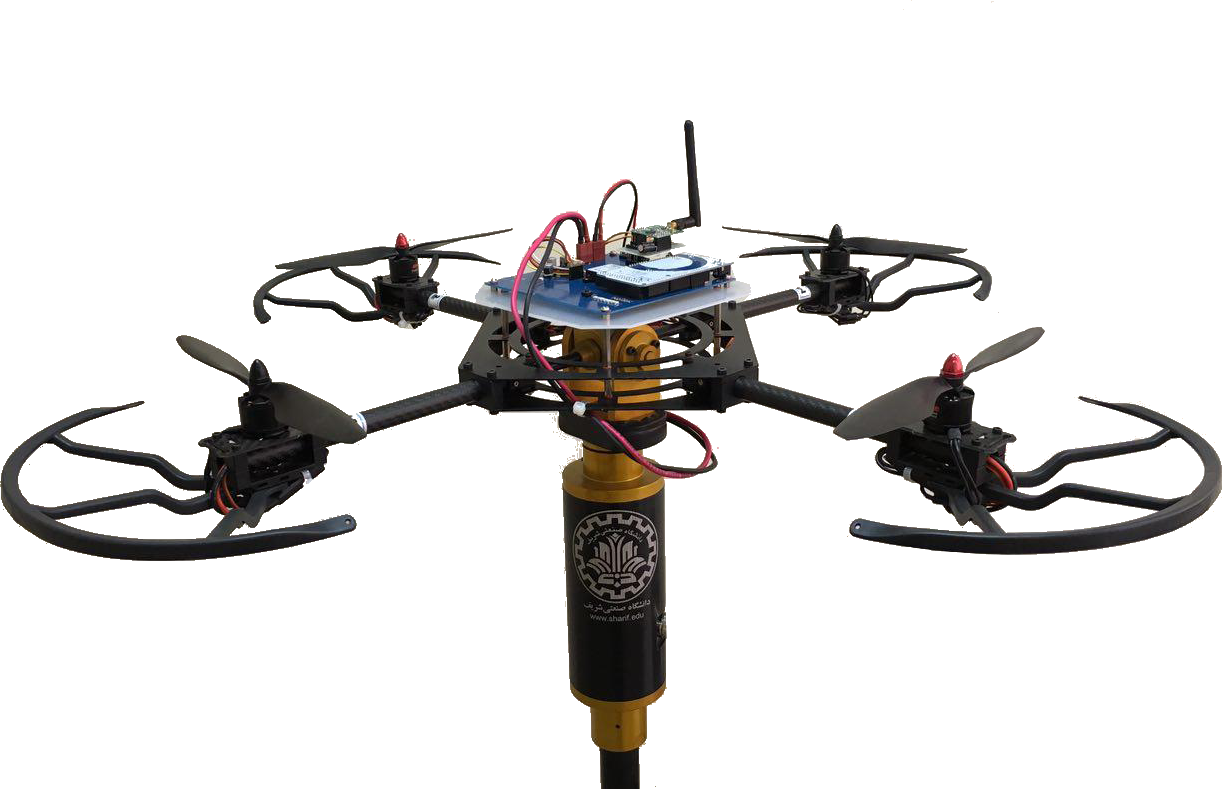
\includegraphics[width=12cm]{../Figures/introduction/3DOFQuad.png}
	\centering
	\caption{استند کنترل وضعیت سه درجه آزادی چهارپره 
	\cite{Iranlabexpo}}
\label{LabQuad1}
\end{figure}
با توجه به شکل
\ref{LabQuad1}،
مرکز جرم این استند بالاتر از مفصل قرار دارد که می‌توان آن را به‌صورت آونگ معکوس در نظر گرفت. بنابراین، سامانه به‌صورت حلقه‌باز ناپایدار است. این سامانه دارای چهار ورودی مستقل (سرعت چرخش پره‌ها) و سه خروجی زوایای اویلر
$(\psi ,\theta ,\phi)$
است. در مدل‌سازی این استند عدم قطعیت وجود دارد; اما، با توجه به کنترل‌کننده مورد استفاده می‌توان این عدم قطعیت را به‌صورت اغتشاش درنظر گرفت و سامانه را به خوبی کنترل کرد. 
%در پایان، با کنترل‌کننده
% تنظیم‌کننده مربعی خطی\LTRfootnote{LQR (Linear Quadratic Regulator)} مقایسه خواهد ‌شد.


%\subsection{ساختار بالگرد}
%
%بالگرد‌ها همانند انواع دیگر وسایل پرنده از ایجاد اختلاف فشار در اتمسفر پیرامون خود و ایجاد نیروی برآ\LTRfootnote{Lift} برای بلندشدن و حرکت در هوا استفاده می‌کنند. به‌دلیل وجود نیروی عمل و عکس‌العمل در بالگردها، پس از اینکه پره اصلی شروع به چرخش می‌کند، با برخورد مولکول‌های هوا به این پره و وجود عکس‌العمل، یک نیرویی با جهت مخالف جهت چرخش پره به پره و در ادامه گشتاوری به شفت متصل به پره اعمال می‌شود و این گشتاور باعث چرخش بالگرد به دور خود می‌شود. در بالگرد برای حل این مشکل، از پره دم استفاده می‌شود تا گشتاوری را تولید کند که مانع چرخش بالگرد به دور خود شود. 
%\begin{figure}[H]
%	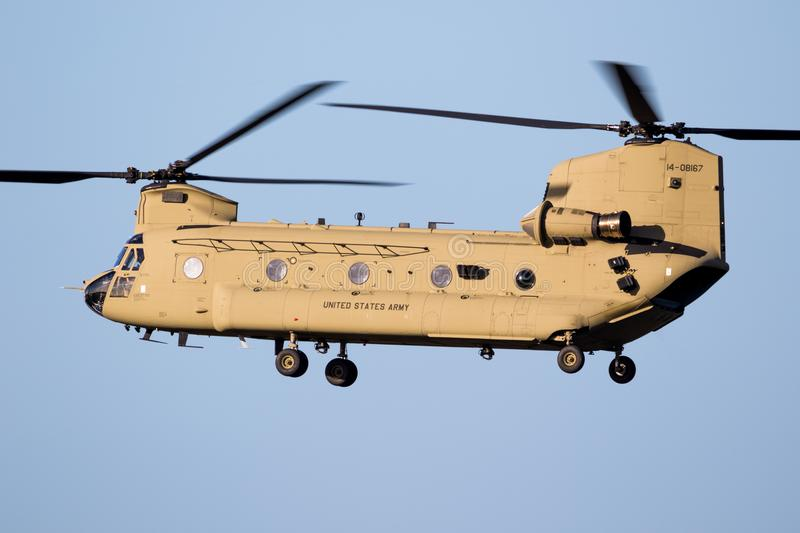
\includegraphics[width=10cm]{../Figures/introduction/boeing-ch-chinook.jpg}
%	\centering
%	\caption{بالگرد شینوک
%		\cite{CH-47}}
%	\label{chinook}
%\end{figure}
%حال اگر بالگرد به جای داشتن یک پره اصلی از دو پره اصلی که خلاف جهت یکدیگر بچرخند استفاده می‌نمود، به‌دلیل خنثی‌شدن دو  گشتاور توسط یکدیگر، دیگر بالگرد به دور خود نمی‌چرخید. مانند بالگردهای شینوک\LTRfootnote{Boeing CH-47 Chinook} که نمایی از آن در شکل
%\ref{chinook}
%آورده شده‌است. حال، با توجه به توضیحات داده‌شده، راحت‌تر می‌توان به ساختار چهارپره‌ها اشاره نمود.
%\subsection{ساختار چهارپره}


چهارپره‌ها با بهره‌گیری از چهار موتور و پره مجزا و چرخش دو به دو معکوس این موتورها، گشتاورهای عکس‌العملی یکدیگر را خنثی می‌کنند و همچنین اختلاف فشار لازم جهت ایجاد نیروی برآ را تأمین می‌کنند.

\begin{figure}[H]
	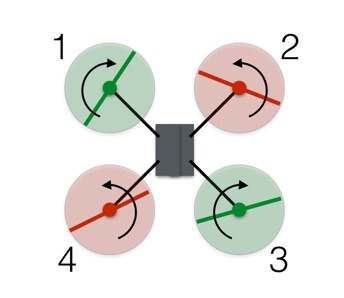
\includegraphics[width=8cm]{../Figures/introduction/Quadblade.jpg}
	\centering
	\caption{جهت چرخش پره‌های چهارپره
		\cite{Quadhowfly}}
\end{figure}

نحوه ایجاد فرامین کنترلی در چهارپره‌ها به این صورت است که برای تغییر ارتفاع از کم یا زیاد کردن سرعت چرخش موتورها استفاده می‌شود و باعث کم یا زیاد شدن نیروی برآ می‌شود. برای چرخش چهارپره به دور خود و به‌صورت درجا، دو پره هم جهت با سرعت کمتر و دو پره هم جهت دیگر با سرعت بیشتر می‌چرخند و گشتاور یاو ایجاد می‌شود و نیروی برآ ثابت می‌ماند؛
%(زیرا دو پره با سرعت کمتر و دو پره دیگر به همان نسبت با سرعت بیشتر می‌چرخند.)
 بنابراین، چهارپره در ارتفاع ثابت به دور خود می‌چرخد. همچنین، با کم و زیاد کردن دو به دو سرعت موتورهای مجاور چهارپره از حالت افقی خارج شده و در صفحه افق حرکت می‌کند.


\section{نظریه بازی}
نظریه بازی با استفاده از مدل‌های ریاضی به تحلیل روش‌های همکاری یا رقابت موجودات منطقی و هوشمند می‌پردازد. نظریه بازی، شاخه‌ای از ریاضیات کاربردی است که در علوم اجتماعی و به ویژه در اقتصاد، زیست‌شناسی، مهندسی، علوم سیاسی، روابط بین‌الملل، علوم رایانه، بازاریابی و فلسفه مورد استفاده قرار می‌گیرد. نظریه بازی در تلاش است تا به وسیله‌ی ریاضیات، رفتار را در شرایط راهبردی یا در یک بازی که در آن موفقیت فرد در انتخاب کردن، وابسته به انتخاب دیگران می‌باشد، برآورد کند.
\subsection{تاریخچه نظریه بازی}
%در سال ۱۹۲۱ یک ریاضی‌دان فرانسوی به نام اِمیل بُرِل برای نخستین بار به مطالعهٔ تعدادی از بازی‌های رایج در قمارخانه‌ها پرداخت و چند مقاله در موردِ آن‌ها نوشت. او در این مقاله‌ها بر قابل پیش‌بینی بودنِ نتایجِ این نوع بازی‌ها از راه‌های منطقی، تأکید کرده بود. 
%کوتاه است یا نه؟؟؟؟؟؟؟؟؟؟؟
در سال ۱۹۹۴ جان فوربز نش به همراه جان هارسانی و راینهارد سیلتن به خاطر مطالعات خلاقانه‌ی خود در زمینه‌ی نظریه بازی، برنده‌ی جایزه نوبل اقتصاد شدند. در سال‌های پس از آن نیز بسیاری از برندگان جایزه‌ی نوبل اقتصاد از میان متخصصین نظریه بازی انتخاب شدند. آخرین آن‌ها، ژان تیرول فرانسوی است که در سال ۲۰۱۴ این جایزه را کسب کرد \cite{nobel}.
\subsection{تعادل نش}
پژوهش‌ها در این زمینه اغلب بر مجموعه‌ای از راهبردهای شناخته شده به عنوان تعادل در بازی‌ها استوار است. این راهبردها به‌طور معمول از قواعد عقلانی به نتیجه می‌رسند. مشهورترین تعادل‌ها، تعادل نش است. 
تعادل نش در بازی‌هایی کاربرد دارد  در آن فرض شده‌است که هر بازیکن به راهبرد تعادل دیگر بازیکنان آگاه است.
%در نظریه بازی، تعادل نش (به نام جان فوربز نش، که آن را پیشنهاد کرد) راه حلی از نظریه بازی است که شامل دو یا چند بازیکن است، که در آن فرض بر آگاهی هر بازیکن به راهبرد تعادل دیگر بازیکنان است. 
بر اساس نظریه‌ی تعادل نش، در یک بازی که هر بازیکن امکان انتخاب‌های گوناگون دارد اگر بازیکنان به روش منطقی  راهبردهای خود را انتخاب کنند و به دنبال حداکثر سود در بازی باشند، دست کم یک راهبرد برای به دست آوردن بهترین نتیجه برای هر بازیکن وجود دارد و چنانچه بازیکن راهکار دیگری را انتخاب کند، نتیجه‌ی بهتری به دست نخواهد آورد.




%\chapter{بازی دیفرانسیلی}
در این قسمت به خلاصه‌ای از بازی دیفرانسیلی پرداخته شده است. تمامی توضیحات و روابط  از منبع 
 \cite{article1}
آورده شده است. در این فصل حالت حلقه‌باز\LTRfootnote{Opne Loop}
 و حالت همراه با بازخورد\LTRfootnote{Feedback} بررسی می‌شود.
 % یا شده است؟
 این پروژه حالت دو بازیکن را بررسی می‌کند. در این مسئله فرض شده  که تابع هزینه برای هر بازیکن به فرم مربعی است. 	هدف اصلی کم کردن تابع هزینه برای بازیکنان است. تابع هزینه به فرم رابطه (\ref{cost}) نوشته می‌شود.

 \begin{equation}\label{cost}
 	J_i(u_1, u_2) = \int_{0}^{T}\left( \boldsymbol{x} ^\mathrm{T}(t) \boldsymbol{Q_i} \boldsymbol{x}(t)+
 	 \boldsymbol{u_i} ^\mathrm{T}(t) \boldsymbol{R_{ii}} \boldsymbol{u_i}(t)+
 	 \boldsymbol{u_j} ^\mathrm{T}(t)\boldsymbol{ Q_{ij} u_j}(t)
 	\right)dt+
 	\boldsymbol{ x} ^\mathrm{T}(T)\boldsymbol{ H_i}\boldsymbol{ x}(T) 
  \end{equation}
در اینجا ماتریس‌های 
$\boldsymbol{Q_i}$ ، $\boldsymbol{R_{ii}}$
و
$\boldsymbol{H}$
متقارن فرض شده‌اند و ماتریس 
$\boldsymbol{R_{ii}}$
به صورت مثبت معین ($\boldsymbol{R_{ii}}>0$)
فرض شده است.
دینامیک سیستم تحت تاثیر هر دو بازیکن قرار می‌گیرد. در اینجا دینامیک سیستم به فرم رابطه (\ref{system_dynamic}) در نظر گرفته شده ‌است.
\begin{equation}\label{system_dynamic}
	\boldsymbol{\dot x}(t) = \boldsymbol{Ax}(t) + \boldsymbol{B_1u_1}(t) + \boldsymbol{B_2u_2}(t), \quad \boldsymbol{x}(0) = \boldsymbol{x}_0
\end{equation}
در رابطه 
(\ref{system_dynamic})،
$\boldsymbol{u_1}$
برابر با تلاش کنترلی بهینه بازیکن اول است. در اینجا ممکن است تلاش کنترلی بازیکن اول موجب دور شدن بازیکن دوم از هدف شود و یا برعکس.  این پروژه حالت همکاری دو بازیکن را بررسی نمی‌کند و دو بازیکن در تلاش برای کم کردن تابع هزینه خود و زیاد کردن تابع هزینه بازیکن مقابل هستند.

%\section{کنترل‌کننده خطی مربعی مبتنی بر بازی دیفرانسیلی}\label{LQDG}
در این حالت فرض شده است که تمامی بازیکنان در زمان 
$t \in [0, T]$
فقط اطلاعات شرایط اولیه و مدل سیستم را دارند. این فرض به این صورت تفسیر می‌شود که دو بازیکن همزمان حرکت خود را در انتخاب می‌کنند. در این حالت امکان هماهنگی بین دو بازیکن وجود ندارد. تعادل نش در ادامه تعریف شده ‌است.
\شروع{قضیه} 
به مجموعه‌ای از حرکات قابل قبول 
$(\boldsymbol{u_1}^*,  \boldsymbol{u_2}^*)$
یک \مهم{تعادل نش} برای بازی می‌گویند اگر تمامی حرکات قابل قبول 
$(\boldsymbol{u_1},  \boldsymbol{u_2})$
از نامساوی (\ref{nash_lqe}) پیروی کنند.
\begin{equation}\label{nash_lqe}
	J_1(\boldsymbol{u_1}^*, \boldsymbol{u_2}^*)\leq J_1(\boldsymbol{u_1}, \boldsymbol{u_2}^*) \text{\rm{ and }}
	J_2(\boldsymbol{u_1}^*, \boldsymbol{u_2}^*)\leq 
	J_2(\boldsymbol{u_1}^*, \boldsymbol{u_2})
\end{equation}
\پایان{قضیه}
در اینجا قابل قبول بودن به‌معنی آن است که
$\boldsymbol{u_i}(.)$
به یک مجموعه محدود حرکات تعلق دارد، این مجموعه‌ی حرکات که بستگی به اطلاعات بازیکنان از بازی دارد، مجموعه‌ای از راهبردهایی است که بازیکنان ترجیح می‌دهند برای کنترل سیستم انجام دهند و سیستم 
(\ref{system_dynamic})
باید یک جواب منحصر به فرد داشته باشد. 


تعادل نش به گونه‌ای تعریف می‌شود که هیچ یک از بازیکنان انگیزه‌ی یک طرفه برای انحراف از بازی ندارند. قابل ذکر است که نمی‌توان انتظار داشت که یک تعادل نش منحصر به فرد وجود داشته باشد. به هر حال به راحتی می‌توان تایید کرد که حرکات
$(\boldsymbol{u_1}^*, \boldsymbol{u_2}^*)$
یک تعادل نش برای بازی با تابع هزینه
$J_i,~ (i = 1, 2)$
است.
 %اگر تعادل نش برای تابع هزینه قسمت قبل برقرار باشد برای تابع هزینه
%$\alpha_iJ_i~ i = 1, 2, ~\alpha_i>0$
%نیز برقرار است.


برای سادگی از نمادسازی 
$\boldsymbol{S_i} := \boldsymbol{B_iR_{ii}}^{-1}\boldsymbol{B_i}^\mathrm{T}$
استفاده شده‌است. در اینجا فرض شده است که زمان $T$ محدود است.
\شروع{قضیه} \label{openlooptheorm}
ماتریس
$\boldsymbol{M}$ را در نظر بگیرید:
\begin{equation}
	\boldsymbol{M} :=
	\begin{bmatrix}
		\boldsymbol{A} & -\boldsymbol{S_1} & -\boldsymbol{S_2}\\
		-\boldsymbol{Q_1} & -\boldsymbol{A}^\mathrm{T}& \boldsymbol{0}\\
		-\boldsymbol{Q_2} & \boldsymbol{0} & -\boldsymbol{A}^\mathrm{T}
	\end{bmatrix}
\end{equation}
فرض شده ‌است که دو معادله دیفرانسیلی ریکاتی
(\ref{riccati_teorm})، 
 در بازه
$[0, T]$
جواب متقارن دارند.
\begin{equation}\label{riccati_teorm}
	\boldsymbol{\dot{K}_i}(t) = -\boldsymbol{A}^\mathrm{T}\boldsymbol{K_i}(t)-\boldsymbol{K_i}(t)\boldsymbol{A}+\boldsymbol{K_i}(t)\boldsymbol{S_iK_i}(t)-\boldsymbol{Q_i},\quad \boldsymbol{K_i}(T) = \boldsymbol{H_i},\quad i = 1, 2
\end{equation}
\newpage
بازی دیفرانسیل خطی درجه دوم دو نفره\LTRfootnote{the two player linear quadratic differential game} تعادل نش حلقه‌باز در هر شرایط اولیه $\boldsymbol{X_0}
$
دارد اگر ماتریس
\begin{equation}
	\boldsymbol{H}(T) := \begin{bmatrix}
		\boldsymbol{I}&0&0
	\end{bmatrix}
e^{-\boldsymbol{M}T}
\begin{bmatrix}
	\boldsymbol{I}
	\\ \boldsymbol{H_{1}}
	\\ \boldsymbol{H_{2}}
\end{bmatrix}
\end{equation}
معکوس‌پذیر‌ باشد
 \cite{article1}
 .
\پایان{قضیه}
در معادلات بالا تلاش کنترلی برای هر بازیکن به فرم رابطه \ref{openloop_u} تعریف شده است.
\begin{equation}\label{openloop_u}
	\boldsymbol{u_i}(t) = -\boldsymbol{R_{ii}}\boldsymbol{B_i}^\mathrm{T}\boldsymbol{x}(t),\quad i = 1, 2
\end{equation}
در آخر با استفاده از قضیه
 \ref{openlooptheorm}
با حل دو معادله کوپل ریکاتی دیفرانسیلی می‌توان به جواب رسید.
\begin{align}
	\boldsymbol{\dot{K}_1} &= -\boldsymbol{A}^\mathrm{T}\boldsymbol{K_1} - \boldsymbol{K_1A} - \boldsymbol{Q_1} +\boldsymbol{K_1S_1K_1} + \boldsymbol{K_1S_2K_2};\quad \boldsymbol{K_1}(T) = \boldsymbol{H_1}\\
	\boldsymbol{\dot{K}_2} &= -\boldsymbol{A}^\mathrm{T}\boldsymbol{K_2} - \boldsymbol{K_2A} - \boldsymbol{Q_2} +\boldsymbol{K_2S_2K_2} + \boldsymbol{K_2S_1K_1};\quad \boldsymbol{K_2}(T) = \boldsymbol{H_2}
\end{align}


%\section{بازی همراه با بازخورد}
تفاوت بازی همراه با بازخورد\LTRfootnote{The Feeback Game} با بازی حلقه‌باز در این است که بازیکنان در هر لحظه از بازی بازخورد می‌گیرند و متناسب با بازخورد رفتار می‌کنند. این بازخورد ممکن است باعث شود یک بازیکن انگیزه پیدا کند که از بازی انحراف پیدا کند در حالی که این اتفاق در بازی حلقه‌باز رخ نمی‌دهد. این اتفاق منجر به یک راه حل تعادلی دیگر می‌شود. از طرف دیگر راه حل تعادلی نباید در طول بازی خودش را با بازکنان سازگار کند.


با توجه به اینکه سیستم خطی است، می‌توان استدلال کرد که حرکات تعادل به صورت تابعی خطی از وضعیت سیستم است. این بدین مفهوم است که تعادل نش باید در فضای ذکر شده باشد. فضای راهبردی
% استراتژی
 به فرم رابطه
 \ref{NashSpace}

\begin{equation}\label{NashSpace}
	\boldsymbol{\Gamma^{lfb}_i} :‌= \left\{\boldsymbol{u_i}(0, T)\vert \boldsymbol{u_i}(t) = \boldsymbol{F_i}(t)\boldsymbol{x}(t) ,~ i = 1, 2\right\}
\end{equation}
تعریف می‌شود. در رابطه
 \ref{NashSpace}
$\boldsymbol{F_i}(.)$
قسمتی از یک تابع است. حرکات تعادل نش
$(\boldsymbol{u_1}^*, \boldsymbol{u_2}^*)$
در فضای استراتژی 
$\boldsymbol{\Gamma^{lfb}_1}\times\boldsymbol{\Gamma^{lfb}_2}$
است.
\شروع{قضیه} 
مجموعه‌ی حرکات کنترلی 
$\boldsymbol{u_i}^*(t)=\boldsymbol{F_i}^*(t)\boldsymbol{x}(t)$
تشکیل شده‌است از بازخورد خطی تعادل نش اگر
\begin{equation*}
	J_1(\boldsymbol{u_1}^*, \boldsymbol{u_2}^*)\leq J_1(\boldsymbol{u_1}, \boldsymbol{u_2}^*)\text{\rm{ and }}
	J_2(\boldsymbol{u_1}^*,\boldsymbol{ u_2}^*)\leq J_2(\boldsymbol{u_1}^*, \boldsymbol{u_2})
\end{equation*}
برای هر 
$\boldsymbol{u_i}\in \boldsymbol{\Gamma^{lfb}_i}$
برقرار باشد.
\پایان{قضیه}
\شروع{قضیه}
بازی دیفرانسیلی خطی درجه دوم دو نفره برای هر شرایط اولیه، تعادل نش خطی بازخورد دارد اگر و فقط اگر مجموعه معادلات کوپل ریکاتی

\begin{align}
	\begin{split}
		\boldsymbol{\dot{K}_1}(t) &= -(\boldsymbol{A}-\boldsymbol{S_2}\boldsymbol{K_2}(t))^\mathrm{T}\boldsymbol{K_1}(t)-\boldsymbol{K_1}(t)(\boldsymbol{A}-\boldsymbol{S_2K_2}(t))+
		\boldsymbol{K_1}(t)\boldsymbol{S_1K_1}(t)-\boldsymbol{Q_1}\\
		\quad \boldsymbol{K_1}(T) &= \boldsymbol{H_1}
	\end{split}\\
	\begin{split}
		\boldsymbol{\dot{K}_2}(t) &= -(\boldsymbol{A}-\boldsymbol{S_1}\boldsymbol{K_1}(t))^\mathrm{T}\boldsymbol{K_2}(t)-\boldsymbol{K_2}(t)(\boldsymbol{A}-\boldsymbol{S_1K_1}(t))+
\boldsymbol{K_2}(t)\boldsymbol{S_2K_2}(t)-\boldsymbol{Q_2}\\
\quad \boldsymbol{K_2}(T) &= \boldsymbol{H_2}
	\end{split}
\end{align}
در بازه زمانی 
$[0, T]$
جواب متقارن داشته ‌باشند (برای سادگی 
$\boldsymbol{S_{12}}=\boldsymbol{S_{21}} =\boldsymbol 0 $
فرض شده است).
در این حالت دارای تعادل منحصر به فرد است. حرکت‌های تعادل به فرم رابطه
\ref{nash_action}
است.
\begin{equation}\label{nash_action}
	\boldsymbol{u_i}^*(t) = -\boldsymbol{R_{ii}B_i}^T\boldsymbol{K_i}(T)\boldsymbol{x}(T),~i = 1, 2
\end{equation}
\پایان{قضیه}

%%%----------section----------------------
%\chapter{مدل‌سازی چهارپره}
 در این فصل به مدلسازی استند چهارپره آزمایشگاهی  پرداخته شده‌است. به این منظور، ابتدا فرضیات مربوط به 
 مدلسازی چهارپره در بخش
\ref{sec_modelassum}
 بیان می‌شود. سپس، در بخش
 \ref{sec:moment}
 معادلات حاکم بر حرکات دورانی چهارپره و در زیر بخش‌های
 \ref{sec:aeromoment},
 \ref{sec:edgemoment},
 \ref{sec:friction}
 و
 \ref{sec:mgmoent}
%  بیان می‌شود. در ادامه،
   به استخراج گشتاورهای خارجی اعمالی 
 به استند شامل گشتاورهای آیرودینامیکی ناشی از پره، گشتاور نیروی تکیه‌گاه، گشتاورهای ناشی از 
 اصطکاک بیرینگ‌ها و  گشتاورهای ناشی از جرم استند پرداخته می‌شود. در گام بعد، در بخش
 \ref{sec:finalrotate}
 معادله نهایی دینامیک دورانی استند 
 استخراج می‌شود. سپس، فرم فضای حالت استند آزمایشگاهی در بخش
 \ref{spacestate}
 استخراج می‌شود. لازم به 
 توضیح است که فرم نهایی فضای حالت استند بدون درنظرگرفتن اصطکاک بیرینگ‌ها از منبع
 \cite{Abeshtan}
 آورده ‌شده‌است که در آن منبع، مدل استخراج‌شده با اعمال ورودی‌ها و شرایط اولیه مختلف 
 اعتبارسنجی شده‌‌است.
%\section{فرضیات مدل‌سازی}
شماتیک استند چهارپره در شكل \ref{QuadAssum}نشان داده شده است. به ‌منظور استخراج معادلات حاکم بر سیستم، 
فرض می‌شود که چهارپره صلب و متقارن است. همچنین ماتریس گشتاور اینرسی چهارپره به صورت قطری درنظر گرفته می‌شود. مرکز ثقل سازه چهارپره روی نقطه $B$ و مرکز ثقل هر یک از پره‌ها به همراه قسمت دوار موتور روی نقاط 
$B_1$
تا
$B_4$
است. مبدأ دستگاه مختصات بدنی روی محل تقاطع بازوهای چهارپره یعنی نقطه 
$B$
در نظر گرفته شده است. از آنجایی ‌که مرکز ثقل پره‌ها بالاتر از مرکز ثقل سازه چهارپره است، مرکز ثقل کلی چهارپره جایی بین مرکز ثقل موتورها و سازه، یعنی نقطه‌ی 
$C$
می‌گیرد. همچنین قابل ذکر است که نقطه‌ی
$D$
محل اتصال کلی استند چهارپره است. جهت مثبت محور 
$X^B$
و
$Y^B$
دستگاه مختصات بدنی به ترتیب در راستای بازوی مربوط به موتور 1 و 4 فرض می‌شود. همچنین جهت مثبت محور
$Z^B$
با توجه به قانون دست راست حاصل می‌شود.
\begin{figure}[H]\label{QuadAssum}
	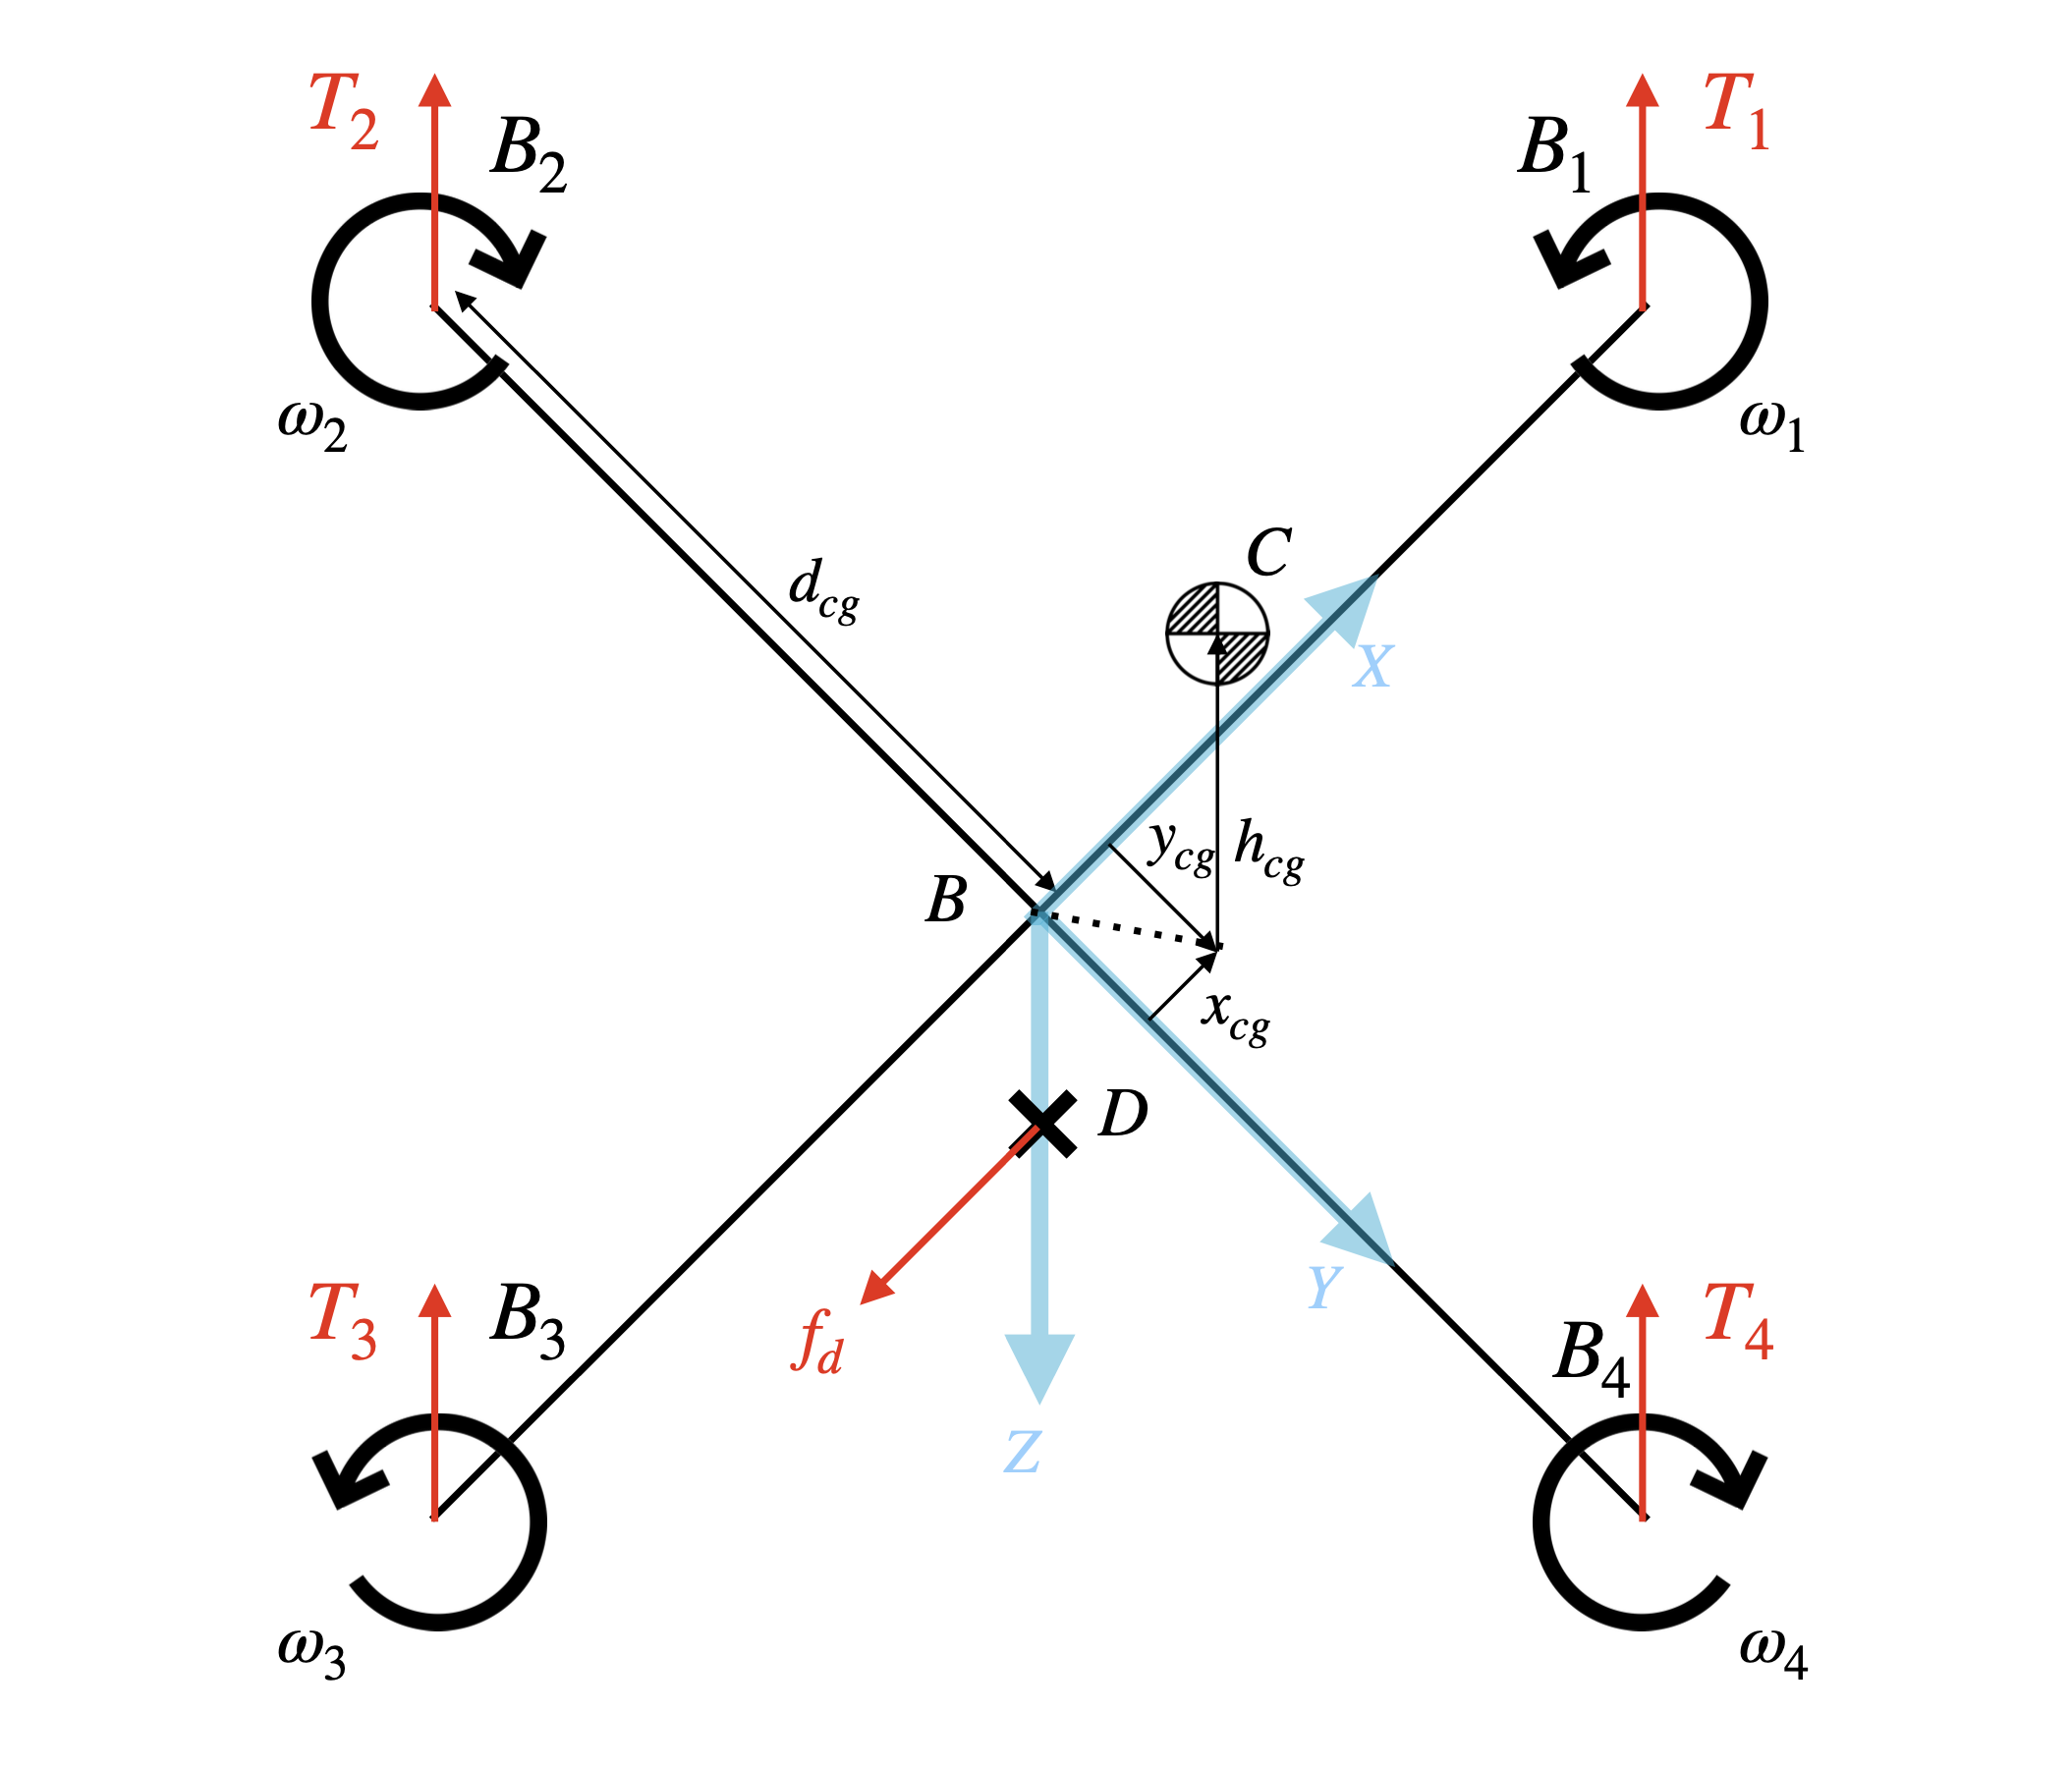
\includegraphics[width=12cm]{../Figures/Forces/StandAssumations.png}
	\centering
	\caption{شماتیک استند چهارپره}
\end{figure}
%\section{معادله گشتاور}\label{sec:moment}
به‌منظور استخراج معادلات حاکم بر حرکت دورانی چهارپره، از قوانین نیوتن-اویلر استفاده می‌شود. از این رو،
معادله دیفرانسیلی اویلر برای یک پرنده حول مرکز ثقل آن در دستگاه مختصات بدنی به صورت زیر بیان می‌شود \cite{zipfel2000modeling}:
\begin{equation}\label{torque}
	\left[\dot{\boldsymbol{\omega}}^{BI}\right]^B = \left(\left[\boldsymbol J\right]^B\right)^{-1}
	\left(-\left[\boldsymbol \Omega^{BI}\right]^B\times\left(
	\left[\boldsymbol J\right]^B\left[\boldsymbol \omega^{BI}\right]^B+
	\left[\boldsymbol I_R\right]^B
	\right)+ \left[\boldsymbol m_b\right]^B\right)
\end{equation}
در رابطه
(\ref{torque})، عبارت 
$\left[\dot{\boldsymbol\omega}^{BI}\right]^B$
بیانگر بردار مشتق نرخ‌های زاویه‌ای چهارپره در دستگاه مختصات بدنی است. همچنین ماتریس 
$\left[\boldsymbol J\right]^B$
نشان‌دهنده گشتاورهای اینرسی چهارپره حول مرکز ثقل آن در دستگاه مختصات بدنی است که به دلیل تقارن چهارپره به صورت زیر درنظر گرفته
 می‌شود:
 \begin{equation}\label{Jmatrix}
 	\left[\boldsymbol J\right]^B = \begin{bmatrix}
 		J_{11} & 0 &0\\
 		0 & J_{22} & 0\\
 		0 & 0 & J_{33}
 	\end{bmatrix}
 \end{equation}
در رابطه 
(\ref{Jmatrix})، پارامترهای 
$J_{11}$،
$J_{22}$
و 
$J_{33}$
به ترتیب بیانگر گشتاور‌های اینرسی چهارپره حول محورهای 
$X^B$،
$Y^B$
و 
$Z^B$
دستگاه مختصات بدنی هستند. همچنین بردار 
$\left[\boldsymbol I_R\right]^B$
در رابطه‌ی 
(\ref{torque})
بیانگر مجموع تكانه زاویه‌ای کلی پره‌ها در دستگاه مختصات بدنی است. ازآنجا که، تكانه زاویه‌ای پره‌ها در راستای محور
$Z^B$
دستگاه مختصات بدنی است؛ در نتیجه 
$\left[\boldsymbol I_R\right]^B$
به صورت زیر حاصل می‌شود:
\begin{equation}\label{IR}
	\left[\boldsymbol I_R\right]^B = 
	\begin{bmatrix}
		0\\0\\l_R
	\end{bmatrix}
\end{equation}
در رابطه‌ی 
(\ref{IR})، 
$l_R$
بیانگر تكانه زاویه‌ای کلی پره‌ها در راستای محور
$Z^B$
دستگاه مختصات بدنی است که به صورت زیر حاصل می‌شود:
\begin{equation}\label{IRomega}
	l_R = J_R\omega_d
\end{equation}
در رابطه‌ی
(\ref{IRomega})، پارامتر
$J_R$
بیانگر ممان اینرسی هر یک از پره‌ها است. همچنین
$\omega_d$
نشان دهنده تفاضل نسبی سرعت‌های زاویه‌ای پره‌ها است که با توجه به شكل
\ref{QuadAssum}
به صورت زیر تعریف می‌شود:
\begin{equation}\label{omega_d}
	\omega_d = -\omega_1 + \omega_2-\omega_3 + \omega_4
\end{equation}
همچنین 
$\left[\boldsymbol m_b\right]^B$
در رابطه‌ی
(\ref{torque})
برآیند گشتاورهای خارجی اعمالی به چهارپره، شامل 
گشتاورهای ناشی از آیرودینامیک پره‌ها و گشتاورهای ناشی از نیروی تكیه‌گاه است که در ادامه به آن پرداخته می‌شود.




%\subsection{گشتاورهای ناشی از آيرودينامیک پره‌ها}\label{sec:aeromoment}
آیرودینامیک پره‌ها باعث ایجاد نیروی برآ و درنتیجه گشتاورهای رول و پیچ ناشی از اختلاف نیروی 
برآ می‌شود. با استفاده از تفاضل نیروی برآی پره‌ها دو گشتاور رول و پیچ ایجاد می‌شود. با توجه به تئوری مومنتوم، نیروی برآی هر پره 
% farsi momentum theory
$(T_i)$
از رابطه‌ی زیر حاصل می‌شود
\cite{Sharifi}:
\begin{equation}\label{trust}
	T_i = b\omega_i^2
\end{equation}
در رابطه
(\ref{trust})
$b$
و 
$\omega_i$
به ترتیب بیانگر فاکتور نیروی برآ و سرعت زاویه‌ای هر پره است؛ بنابراین مطابق شکل 
\ref{QuadAssum}
گشتاور رول حول محور
$X^B$
دستگاه مختصات بدنی از رابطه زیر حاصل می‌شود.
\begin{equation}\label{roll}
	m_X^B = d_{cg}(T_2-T_4) = d_{cg}b(\omega_2^2-\omega_4^2)
\end{equation}
در رابطه 
(\ref{roll})
عبارت 
$d_{cg}$
بیانگر فاصله مرکز هر پره از مرکز جرم چهارپره در راستای محور
$X^B$
دستگاه مختصات بدنی است. همچنین گشتاور پیچ حول محور 
$Y^B$
دستگاه مختصات بدنی با توجه به شكل
\ref{QuadAssum}
از رابطه زیر حاصل می‌شود:
\begin{equation}\label{pitch}
	m_Y^B = d_{cg}(T_1-T_3) = d_{cg}b(\omega_1^2-\omega_3^2)
\end{equation}
گشتاور یاو آیرودینامیكی از اختلاف گشتاور ناشی از پسای پره‌ها ایجاد می‌شود؛ بنابراین، جهت این 
گشتاور همواره در جهت مخالف چرخش پره‌ها است. بنابراین، گشتاور یاو حول محور
$Z^B$
دستگاه مختصات بدنی با توجه به شكل
\ref{QuadAssum},
مطابق رابطه زیر حاصل می‌شود:
\begin{equation}\label{yaw}
	m_Z^B = d(\omega_1^2-\omega_2^2+\omega_3^2-\omega_4^2)
\end{equation}
رابطه 
(\ref{yaw})
عبارت 
$d$
بیانگر فاکتور گشتاور پسای پره‌ها است. در نتیجه با توجه به معادلات
(\ref{roll}),
(\ref{pitch})
و
(\ref{yaw})
بردار گشتاورهای خارجی ناشی از آیرودینامیک پره‌ها در دستگاه مختصات بدنی به صورت زیر حاصل می‌شود:
\begin{equation}\label{finaltorque}
	\left[m_A\right]^B = \begin{bmatrix}
		m_X^B\\m_Y^B\\m_Z^B
	\end{bmatrix}
 =  \begin{bmatrix}
 	d_{cg}b(\omega_2^2-\omega_4^2)\\
 	d_{cg}b(\omega_1^2-\omega_3^2)\\
 	d(\omega_1^2-\omega_2^2+\omega_3^2-\omega_4^2)
 \end{bmatrix}
\end{equation}
%\section{گشتاور ناشی از نیروی تكیه‌گاه}
همانطور که در شكل \ref{QuadAssum} مشاهده می‌شود، نیروی
$f_d$
که در نقطه‌ی 
$D$
از طرق اتصال کلی به چهارپره وارد می‌شود، باعث ایجاد گشتاوری حول مرکز ثقل چهارپره می‌شود. به منظور مدل‌سازی گشتاور ناشی از این نیرو حول نقطه
$C$
، لازم است ابتدا نیروی
$f_d$
استخراج شود. از انجایی که نقطه‌ی
$D$
منطبق بر مرکز ثقل چهارپره نیست؛ لذا معادله حرکت انتقالی برای نقطه اتصال
$D$
با استفاده از معادله انتقال یافته نیوتن (معادله گروبین) به صورت معادله زیر حاصل می‌شود
\cite{zipfel2000modeling}
:
\begin{equation}\label{oprigintorque}
	m_{tot} \left[D^Iv_D^I\right]^B = 
	\left[\Sigma f\right]^B-m_{tot}\left\{
	\left[\Omega^{BI}\right]^B
	\left[\Omega^{BI}\right]^B
	\left[s_{cd}\right]^B+
	\left[D^I\Omega^{BI}\right]^B
	\left[s_{cd}\right]^B
	\right\}
\end{equation}
در رابطه
\ref{oprigintorque}، 
$m_{tot}$
مجموع جرم چهارپره و 
$\left[D^Iv_D^I\right]^B$
مشتق دورانی سرعت نقطه
$D$
نسبت به قاب اینرسی در دستگاه مختصات بدنی است. همچنین
$\left[\Sigma f\right]^B$
بیان‌کننده برآیند نیروهای وارده بر نقطه‌ی
$D$
و
$\left[D^I\Omega^{BI}\right]^B$
ماتریس پادمتقارن بردار سرعت زاوی‌های چهارپره نسبت به قاب اینرسی در دستگاه مختصات بدنی است. همچنین
$\left[D^I\Omega^{BI}\right]^B$
نشان‌دهنده مشتق دورانی سرعت زاوی‌های چهارپره نسبت به قاب اینرسی و 
$\left[s_{cd}\right]^B$
بردار واصل از نقطه‌ی
$D$
به نقطه
$C$
با انتقال قاب بدنی به قاب اینرسی، معادله 
\ref{oprigintorque}
به صورت زیر حاصل می‌شود:
\begin{equation}
\begin{split}\label{newoprigintorque}
	&m_{tot} \left[D^Bv_D^I\right]^B +
	m_{tot}\left[\Omega^{BI}\right]^B
	\left[v_D^{I}\right]^B = \\
	&\left[\Sigma f\right]^B-m_{tot}\left\{2
	\left[\Omega^{BI}\right]^B
	\left[\Omega^{BI}\right]^B
	\left[s_{cd}\right]^B+
	\left[D^I\Omega^{BI}\right]^B
	\left[s_{cd}\right]^B
	\right\}
\end{split}
\end{equation}
همچنین به دلیل اینكه سرعت محل اتصال چهارپره(نقطه
$D$)
صفر است؛ دو عبارت سمت چپ معادله
\ref{newoprigintorque} 
هر دو صفر هستند. در نتیجه معادله به صورت زیر ساده می‌شود.
\begin{equation}\label{newnewoprigintorque}
	\left[\Sigma f\right]^B - 
	m_{tot}\left\{2
	\left[\Omega^{BI}\right]^B
	\left[\Omega^{BI}\right]^B
	\left[s_{cd}\right]^B+
	\left[\dfrac{d\Omega^{BI}}{dt}\right]^B
	\left[s_{cd}\right]^B
	\right\}
\end{equation}
عبارت 
$\left[\Sigma f\right]^B$
بیانگر مجموع نیروهای وارد بر چهارپره است که به صورت معادله زیر بیان می‌شود:
\begin{equation}\label{sigmaF}
	\left[\Sigma f\right]^B = \left[f_D\right]^B+\left[f_T\right]^B+
	\left[f_G\right]^B
\end{equation}
در رابطه 
\ref{sigmaF}، بردار 
$\left[f_D\right]^B$
مقدار نیروی اعمال‌ شده توسط اتصال کلی در نقطه‌ی
$D$
است. همچنین  بردار 
$\left[f_T\right]^B$
بیانگر مدموع نیروی تراست پرهها در دستگاه مختصات بدنی است که از رابطه زیر حاصل می‌شود:
\begin{equation}\label{trustmatrix}
	\left[f_G\right]^B = \begin{bmatrix}
		0\\0\\
		T_1+T_2+T_3+T_4
	\end{bmatrix}
\end{equation}
مقدار نیروی اعمال‌ شده توسط اتصال کلی در نقطه‌ی
$D$
است. همچنین  بردار 
$\left[f_G\right]^B$
بیانگر نیروی وزن چهارپره در دستگاه مختصات بدنی است که از رابطه زیر حاصل می‌شود:
\begin{equation}\label{fg}
	\left[f_G\right]^B = \left[C\right]^{BL}
	\left[f_G\right]^L
\end{equation}
در رابطه
\ref{fg}،
ماتریس انتقال از دستگاه مختصات تراز محلی
$(L)$
 به دستگاه مختصات بدنی است. با جایگذاری روابط
\ref{newnewoprigintorque}،
\ref{sigmaF}،
\ref{trustmatrix}و
\ref{fg}
عبارت زیر برای نیروی تكیه‌گاهی حاصل می‌شود.
\begin{equation}\label{originnew}
	\left[f_D\right]^B = 
	-\left[f_G\right]^B-
	\left[f_T\right]^B+
	m_{tot}\left\{2
	\left[\Omega^{BI}\right]^B
	\left[\Omega^{BI}\right]^B
	\left[s_{cd}\right]^B+
	\left[\dfrac{d\Omega^{BI}}{dt}\right]^B
	\left[s_{cd}\right]^B
	\right\}
\end{equation}
سپس از حاصل‌ضرب نیروی تكیه‌گاه مدل‌ شده در معادله
\ref{originnew}
 در بردار محل اثر آن، گشتاور ایجاد شده
توسط نیروی اتصال کلی به صورت معادله زیر حاصل می‌شود:
\begin{equation}\label{universaltor}
	\left[m_d\right]^B = \left[s_{DC}\right]^B\left(
	-\left[f_G\right]^B
	-\left[f_T\right]^B
	m_{tot}\left\{2
	\left[\Omega^{BI}\right]^B
	\left[\Omega^{BI}\right]^B
	\left[s_{cd}\right]^B
	\right\}
	\right)
\end{equation}
در رابطه
\ref{universaltor}
بردار 
$\left[s_{DC}\right]^B$
بیانگر فاصله‌ی نقطه‌ی 
$D$
از مرکز ثقل چهارپره 
$(h_{cg})$
است که به صورت زیر بیان می‌شود:
\begin{equation}
	\left[s_{DC}\right]^B = \begin{bmatrix}
		0\\0\\h_{cg}
	\end{bmatrix}
\end{equation}
 درنتیجه با جمع گشتاورهای ناشی از نیروهای آیرودینامیک پره‌ها از معادله 
 \ref{finaltorque}
 و گشتاور ناشی 
از نیروی تكیه‌گاه از معادله 
\ref{universaltor}، گشتاور خارجی کلی اعمالی به چهارپره به صورت معادله زیر حاصل 
می‌شود:
\begin{equation}\label{finalm}
	\left[m_B\right]^B = 
	\left[m_A\right]^B+
	\left[m_D\right]^B
\end{equation}


%\section{گشتاورهای ناشی از اصطكاک بیرينگ‌ها}
هر یک از محورهای استند آزمایشگاهی به‌وسیله بیرینگ به‌یکدیگر متصل شدهاند. گشتاور ناشی ازاصطکاک بیرینگها در استند را میتوان به‌صورت زیر مدل کرد
\cite{Arabolye}
:
%site alizad
\begin{equation}\label{friction}
	[\boldsymbol m_f]^B = \begin{bmatrix}
		P_1\mu_sr_x \\
		P_2\mu_sr_y \\
		P_3\mu_sr_z
	\end{bmatrix} + \begin{bmatrix}
	P_1\mu_kr_x \\
	P_2\mu_kr_y \\
	P_3\mu_kr_z
\end{bmatrix}
\end{equation}
در رابطه \ref{friction}، $\boldsymbol P$ نیروی عمودی وارد بر تکیه‌گاه هر یک از محورها، $\mu_s$ و $\mu_k$ به‌ترتیب ضریب اصطکاک
ایستایی و دینامیکی بیرینگ‌ها و r شعاع هر یک از بیرنگ‌ها است.

%\subsection{گشتاورهای ناشی از جرم استند}\label{sec:mgmoent}
بر اساس شکل
\ref{QuadAssum}،
مرکز جرم چهارپره با مرکز تقارن چهارپره فاصله دارد. بنابراین، این فاصله باعث به وجود آمدن گشتاور می‌شود.
\begin{equation}\label{mg}
	[\boldsymbol m_ {cg}]^B = \begin{bmatrix}
		m_{tot}gy_{cg} \\
		-m_{tot}gx_{cg} \\
		0
	\end{bmatrix}
\end{equation}
در رابطه
(\ref{mg})،
$x_{cg}$
و
$y_{cg}$
به‌ترتیب فاصله مرکز جرم از محور $Y$ و $X$ است.
%\subsection{ استخراج معادله نهایی دينامیک دورانی}
در این بخش، گشتاورهای خارجی چهارپره و تكانه زاوی‌های کلی پره‌ها در معادله دیفرانسیل اویلر 
جایگذاری شده و شكل نهایی معادله دیفرانسیل استند چهارپره حاصل می‌شود. با جایگذاری مقدار 
گشتاورهای اعمالی به چهارپره از معادله
\ref{finalm}
در معادله 
\ref{torque}
رابطه موردنیاز برای مدل‌سازی
دینامیک دورانی استند بهصورت معادله زیر حاصل می‌شود:
\begin{equation}\label{demifinalrotation}
	\begin{split}
		\left[\dfrac{d\omega^{BI}}{dt}\right]^B = 
		\left(\left[J\right]^B\right)^{-1}\Bigg(
		-&\left[\Omega^{BI}\right]\times\left(
		\left[J\right]^B\left[\omega^{BI}\right]^B
		+\left[I_R\right]^B\right) + \\
		&\left[m_A\right]^B+\left[s_{DC}\right]^B
		\bigg(-\left[G\right]^B
		-\left[T\right]^B+ \\
		&m_{tot}\Bigl\{2
		\left[\Omega^{BI}\right]^B
		\left[\Omega^{BI}\right]^B
		\left[s_{cd}\right]^B+
		\left[\dfrac{d\Omega^{BI}}{dt}\right]^B
		\left[s_{cd}\right]^B
		\Bigr\}\bigg)\Bigg)
	\end{split}
\end{equation}
در رابطه
\ref{demifinalrotation}،
عبارت
$\left[\dfrac{d\Omega^{BI}}{dt}\right]^B$
بیانگر ماتریس پادمتقارن بردار مشتق سرعت‌ زاویه‌ای بدنی
$\left[\dfrac{d\omega^{BI}}{dt}\right]^B$
است. جمله آخر در معادله فوق را می‌توان به صورت زیر بازنویسی کرد:
\begin{equation}\label{sc}
	m_{tot}\left[s_{DC}\right]^R
	\left[\dfrac{d\Omega^{BI}}{dt}\right]^B\left[s_{CD}\right]^R = 
	m_{tot}\left[s_{DC}\right]^R\left[s_{DC}\right]^R
	\left[\dot{\omega}^{BI}\right]^B
\end{equation}
با جایگذاری معادله
\ref{sc}
در معادله
\ref{demifinalrotation}
و ساده سازی بردار سرعت زاویه‌ای پرنده به صورت زیر حاصل می‌شود:
\begin{equation}\label{finaltorquefinal}
	\begin{split}
		\left[\dfrac{d\omega^{BI}}{dt}\right]^B &= A^{-1}b\\
		A &= I - m_{tot}\left(\left[J\right]^B\right)^{-1}
		\left[s_{DC}\right]^B
		\left[s_{DC}\right]^B\\
		b = \left(\left[J\right]^B\right)^{-1}\Bigg(
		-&\left[\Omega^{BI}\right]\times\left(
		\left[J\right]^B\left[\omega^{BI}\right]^B
		+\left[I_R\right]^B\right) + \\
		&\left[m_A\right]^B+\left[s_{DC}\right]^B
		\bigg(-\left[G\right]^B
		-\left[T\right]^B+ \\
		&m_{tot}\Bigl\{2
		\left[\Omega^{BI}\right]^B
		\left[\Omega^{BI}\right]^B
		\left[s_{cd}\right]^B+
		\left[\dfrac{d\Omega^{BI}}{dt}\right]^B
		\left[s_{cd}\right]^B
		\Bigr\}\bigg)\Bigg)		
	\end{split}
\end{equation}
با جایگذاری معادلات بدست آمده در معادله
\ref{finaltorquefinal}
مؤلفه‌های بردار مشتق سرعت زاویه‌ای چهارپره به صورت زیر حاصل می‌شود:
\begin{align}
	\begin{split}
		\dot{p} =& \dfrac{h_{cg}gm_{dot}\cos(\theta)\sin(\phi)
			+\left(J_{22} - J_{33} +2m_{tot}h_{ch}^2\right)qr
		}
		{m_{tot}h_{cg}^2 + J_{11}} \\
		&+\dfrac{bd_{cg}\left(\omega_2^2-\omega_4^2\right) + qJ_R(\omega_1-\omega_2+\omega_3-\omega_4)}
		{m_{tot}h_{cg}^2 + J_{11}}
	\end{split}\\[1em]
		\begin{split}
		\dot{q} =& \dfrac{h_{cg}gm_{dot}\sin(\theta)
			+\left(J_{33} - J_{11} +2m_{tot}h_{ch}^2\right)pr
		}
		{m_{tot}h_{cg}^2 + J_{11}} \\
		&+\dfrac{bd_{cg}\left(\omega_1^2-\omega_3^2\right) - pJ_R(\omega_1-\omega_2+\omega_3-\omega_4)}
		{m_{tot}h_{cg}^2 + J_{11}}
	\end{split}\\[1em]
	\begin{split}
		\dot{r} =& \dfrac{pq(J_{11}-J_{22})
		+ d(\omega_1^2-\omega_2^2+\omega_3^2-\omega_4^2)
	}{J_{33}}
	\end{split}
\end{align}
به منظور انتشار وضعیت دورانی چهارپره، از روش انتشار اویلر استفاده می‌شود. در این‌صورت
\cite{zipfel2000modeling}
:
$$\dot\phi = p + q\sin(\phi)\cos(\theta) +‌
r\cos(\phi)\tan(\theta)
$$
$$
\dot \theta = q\cos(\phi) - r\sin(\phi)
$$
$$
\dot\psi = (q\sin(phi)) + r\cos(\phi))\sec(\theta) 
$$


%\section{استخراج فرم فضای حالت}\label{spacestate}
به منظور استخراج فرم فضای حالت، متغیرهای حالت استند سه درجه آزادی چهارپره به صورت زیر تعریف می‌شود:
\begin{equation}
	\begin{bmatrix}
		x_1\\x_2\\x_3\\x_4\\x_5\\x_6\\
	\end{bmatrix} = 
\begin{bmatrix}
	\phi\\ \theta \\ \psi \\ p\\ q\\ r
\end{bmatrix}
\end{equation}
معادلات ارائه شده به فرم زیر برای فضای حالت بازنویسی شدند:
\begin{equation}
	\dot x_1 = x_4 + x_5\sin(x_1)\tan(x_2) + x_6\cos(x_1)\tan(x_2)
\end{equation}
\begin{equation}
	\dot x_2 = x_5\cos(x_1)- x_6\sin(x_1)
\end{equation}
\begin{equation}
	\dot x_3 = (x_5\sin(x_1) + x_6\cos(x_1))\sec(x_2)
\end{equation}
\begin{equation}
	\dot x_4 = A_1\cos(x_2)\sin(x_1) + 
	A_2x_5x_6 + A_3\left(\omega_2^2-\omega_4^2\right)+
	A_4x_5\left(\omega_1-\omega_2+\omega_3-\omega_4\right)
\end{equation}
\begin{equation}
	\dot x_5 = B_1\sin(x_2) + 
	B_2x_4x_6 + B_3\left(\omega_1^2-\omega_3^2\right)+
	B_4x_4\left(\omega_1-\omega_2+\omega_3-\omega_4\right)
\end{equation}
\begin{equation}
	\dot x_6 = C_1x_4x_5 + 
	C_2\left(\omega_1^2-\omega_2^2+\omega_3^2-\omega_4^2\right)
\end{equation}
ثابت‌های معادلات بالا  به صورت زیر تعریف می‌شوند:
\begin{align*}
	&A_1  = \dfrac{h_{cg}gm_{tot}}{m_{tot}h_{cg}^2+J_{11}}
	&A_2  = \dfrac{2m_{tot}h_{cg}^2+J_{22}-J_{33}}{m_{tot}h_{cg}^2+J_{11}}\quad
	&A_3  = \dfrac{d_{cg}}{m_{tot}h_{cg}^2+J_{11}}
	&A_4  = \dfrac{J_R}{m_{tot}h_{cg}^2+J_{11}}\\
	&B_1  = \dfrac{h_{cg}gm_{tot}}{m_{tot}h_{cg}^2+J_{22}}
	&B_2  = \dfrac{-2m_{tot}h_{cg}^2-J_{11}+J_{33}}{m_{tot}h_{cg}^2+J_{22}}\quad
	&B_3  = \dfrac{d_{cg}}{m_{tot}h_{cg}^2+J_{22}}
	&B_4  = \dfrac{-J_R}{m_{tot}h_{cg}^2+J_{22}}
\end{align*}
\begin{align*}
	C_1 =\dfrac{J_{11}-J_{22}}{J_{33}}\quad
	C_2 =\dfrac{d}{J_{33}}
\end{align*}
به منظور شبیه‌سازی ، پارامترهای استند به صورت جدول 
\ref{parameterstable}
درنظر گرفته شده است که 
مقدار پارامترهای استند آزمایشگاه است.
\begin{table}[H]
	\caption {پارامترهای شبیه‌سازی استند چهارپره \cite{norian}} 
	\label{parameterstable}
	\begin{center}
		\begin{tabular}{ c c c }
			\hline
	پارامتر & واحد & مقدار پارامتر استند چهارپره    \\
			\hline
			$h_{cg}$ & $m$  &$0.02$   \\
			%\hline
			$m_{tot}$ & $kg$& $0.638$    \\
			%\hline
			$J_{11}$ & $kg.m^2$& $0.02839$    \\
			%\hline
			$J_{22}$ & $kg.m^2$& $0.03066$   \\
%			\hline
			$J_{33}$ & $kg.m^2$&$0.0439$    \\
%			\hline
			$b$ &  $1$ &$3.13\times10^{-5}$   \\
%			\hline
			$d_{cg}$ & $m$ &$0.2$     \\
%			\hline
			$d$ & $1$&$3.2\times10^{-6}$   \\
			\hline
		\end{tabular}
	\end{center}
\end{table}



%% -------------------- Chapters --------------------
%\section{خطی‌سازی}
با استفاده از فرم فضای‌حالت استخراج شده در بخش 
\ref{spacestate}
در این قسمت خطی‌سازی انجام شده‌است. در قسمت 
\ref{lin_MIMO}
به صورت چند ورودی و چند خروج
\LTRfootnote{MIMO}
ی برای سرعت دورانی پره‌ها در  
\lr{2000 RPM}
و حول نقطه صفر خطی‌سازی انجام شد. در قسمت بعد مسئله به صورت یک ورودی و یک خروجی 
\LTRfootnote{SISO}
حول نقطه صفر خطی‌سازی انجام شد. در این قسمت برای فازهای مختلف ورودی و یک خروجی در نظر گرفته‌شده‌است و برای فازهای رول، پیچ و یاو مسئله حل شده‌است  سپس از مجموع خروجی‌های بدست‌آمده خروجی کلی یعنی سرعت دورانی پره‌ها بدست‌آمده‌است.
%\subsection{خطی‌سازی به فرم چند ورودی چند خروجی}\label{lin_MIMO}
در این قسمت با توجه به فضای حالت بدست آمده، چهارپره حول نقطه کار خطی‌سازی می‌شود.
\begin{equation*}
	\sigma_1 = \omega_2^2-\omega_4^2,\quad \sigma_2 = \omega_1^2-\omega_3^2,
	\quad \sigma_3 = \omega_1^2-\omega_2^2+\omega_3^2-\omega_4^2,\quad \sigma_4 = \omega_1-\omega_2+\omega_3-\omega_4
\end{equation*}
\begin{equation*}
		\boldsymbol a = \begin{bmatrix}
%		x_4 + x_5\sin(x_1)\tan(x_2) + x_6\cos(x_1)\tan(x_2)\\
%		x_5\cos(x_1)- x_6\sin(x_1)\\
%		(x_5\sin(x_1) + x_6\cos(x_1))\sec(x_2)\\
%		A_1\cos(x_2)\sin(x_1) + 
%		A_2x_5x_6 + A_3\left(\omega_2^2-\omega_4^2\right)+
%		A_4x_5\left(\omega_1-\omega_2+\omega_3-\omega_4\right)- \dfrac{x_4}{\lvert x_4\rvert}A_5+A_6\cos(x_1)\\
%		B_1\sin(x_2) + 
%		B_2x_4x_6 + B_3\left(\omega_1^2-\omega_3^2\right)+
%		B_4x_4\left(\omega_1-\omega_2+\omega_3-\omega_4\right)- \dfrac{x_5}{\lvert x_5\rvert}B_5 + B_6\cos(x_2)\\
%		C_1x_4x_5 + 
%		C_2\left(\omega_1^2-\omega_2^2+\omega_3^2-\omega_4^2\right)- \dfrac{x_6}{\lvert x_6\rvert}C_3
		x_4 + x_5\sin(x_1)\tan(x_2) + x_6\cos(x_1)\tan(x_2)\\
		x_5\cos(x_1)- x_6\sin(x_1)\\
		(x_5\sin(x_1) + x_6\cos(x_1))\sec(x_2)\\
		A_1\cos(x_2)\sin(x_1) + 
		A_2x_5x_6 + A_3\sigma_1+
		A_4x_5\sigma_4- \dfrac{x_4}{\lvert x_4\rvert}A_5+A_6\cos(x_1)\\
		B_1\sin(x_2) + 
		B_2x_4x_6 + B_3\sigma_2+
		B_4x_4\sigma_4- \dfrac{x_5}{\lvert x_5\rvert}B_5 + B_6\cos(x_2)\\
		C_1x_4x_5 + 
		C_2\sigma_3- \dfrac{x_6}{\lvert x_6\rvert}C_3
	\end{bmatrix}
\end{equation*} 
\begin{equation}
	\boldsymbol{x} = \begin{bmatrix} % bold or vec???????????/
		\phi& \theta & \psi & p& q& r
	\end{bmatrix}^\mathrm{T}
\end{equation}
\begin{equation}
	\boldsymbol{\omega} = \begin{bmatrix}
		\omega_1&\omega_2&\omega_3&\omega_4
	\end{bmatrix}^\mathrm{T}
\end{equation}
برای خطی سازی از بسط تیلور استفاده شده ‌است.
\begin{equation}
	\delta \dot{\boldsymbol{x}} = \dfrac{\partial  \boldsymbol a}{\partial  \boldsymbol x}\delta \boldsymbol x + \dfrac{\partial \boldsymbol a}{\partial \boldsymbol \omega}\delta \boldsymbol \omega 
\end{equation}
\begin{equation}
	\dot{\boldsymbol{x}} =
	\begin{bmatrix}
		\delta \dot x_1&
		\delta \dot x_2&
		\delta \dot x_3&
		\delta \dot x_4&
		\delta \dot x_5&
		\delta \dot x_6
	\end{bmatrix}^\mathrm{T}
\end{equation}

\begin{equation}
	\boldsymbol A = \dfrac{\partial \boldsymbol a}{\partial  \boldsymbol x} =
	\begin{bmatrix}
\dfrac{\partial  a_1}{\partial  x_1}&
\dfrac{\partial  a_1}{\partial  x_2}&
\dfrac{\partial  a_1}{\partial  x_3}&
\dfrac{\partial  a_1}{\partial  x_4}&
\dfrac{\partial  a_1}{\partial  x_5}&
\dfrac{\partial  a_1}{\partial  x_6}
\\[1em]
\dfrac{\partial  a_2}{\partial  x_1}&
\dfrac{\partial  a_2}{\partial  x_2}&
\dfrac{\partial  a_2}{\partial  x_3}&
\dfrac{\partial  a_2}{\partial  x_4}&
\dfrac{\partial  a_2}{\partial  x_5}&
\dfrac{\partial  a_2}{\partial  x_6}
\\[1em]
\dfrac{\partial  a_3}{\partial  x_1}&
\dfrac{\partial  a_3}{\partial  x_2}&
\dfrac{\partial  a_3}{\partial  x_3}&
\dfrac{\partial  a_3}{\partial  x_4}&
\dfrac{\partial  a_3}{\partial  x_5}&
\dfrac{\partial  a_3}{\partial  x_6}
\\[1em]
\dfrac{\partial  a_4}{\partial  x_1}&
\dfrac{\partial  a_4}{\partial  x_2}&
\dfrac{\partial  a_4}{\partial  x_3}&
\dfrac{\partial  a_4}{\partial  x_4}&
\dfrac{\partial  a_4}{\partial  x_5}&
\dfrac{\partial  a_4}{\partial  x_6}
\\[1em]
\dfrac{\partial  a_5}{\partial  x_1}&
\dfrac{\partial  a_5}{\partial  x_2}&
\dfrac{\partial  a_5}{\partial  x_3}&
\dfrac{\partial  a_5}{\partial  x_4}&
\dfrac{\partial  a_5}{\partial  x_5}&
\dfrac{\partial  a_5}{\partial  x_6}
\\[1em]
\dfrac{\partial  a_6}{\partial  x_1}&
\dfrac{\partial  a_6}{\partial  x_2}&
\dfrac{\partial  a_6}{\partial  x_3}&
\dfrac{\partial  a_6}{\partial  x_4}&
\dfrac{\partial  a_6}{\partial  x_5}&
\dfrac{\partial  a_6}{\partial  x_6}
	\end{bmatrix}
\end{equation}
\begin{equation}
	 \dfrac{\partial \boldsymbol{ a}}{\partial  x_1} = 
	 \begin{bmatrix}
	 	x_5 \,\mathrm{cos}\left(x_1 \right)\,\mathrm{tan}\left(x_2 \right)-x_6 \,\mathrm{sin}\left(x_1 \right)\,\mathrm{tan}\left(x_2 \right)\\
	 	-x_6 \,\mathrm{cos}\left(x_1 \right)-x_5 \,\mathrm{sin}\left(x_1 \right)\\[0.5em]
	 	\dfrac{x_5 \,\mathrm{cos}\left(x_1 \right)-x_6 \,\mathrm{sin}\left(x_1 \right)}{\mathrm{cos}\left(x_2 \right)}\\
	 	A_1 \,\mathrm{cos}\left(x_1 \right)\,\mathrm{cos}\left(x_2 \right)\\
	 	0\\
	 	0
	 \end{bmatrix}
\end{equation}
\begin{equation}
	\dfrac{\partial \boldsymbol{ a}}{\partial  x_2} = 
	\begin{bmatrix}
	\dfrac{x_6 \,\mathrm{cos}\left(x_1 \right)}{{\mathrm{cos}\left(x_2 \right)}^2 }+\dfrac{x_5 \,\mathrm{sin}\left(x_1 \right)}{{\mathrm{cos}\left(x_2 \right)}^2 }\\
	0\\[0.5em]
	\dfrac{\mathrm{tan}\left(x_2 \right)\,{\left(x_6 \,\mathrm{cos}\left(x_1 \right)+x_5 \,\mathrm{sin}\left(x_1 \right)\right)}}{\mathrm{cos}\left(x_2 \right)}\\
	-A_2 \,\mathrm{sin}\left(x_1 \right)\,\mathrm{sin}\left(x_2 \right)\\
	B_1 \,\mathrm{cos}\left(x_2 \right)\\
	0
	\end{bmatrix}
\end{equation}
\begin{equation}
	\dfrac{\partial \boldsymbol{ a}}{\partial  x_3} = 
	\begin{bmatrix}
		0\\0\\0\\0\\0\\0
	\end{bmatrix}
\end{equation}
\begin{equation}
	\dfrac{\partial \boldsymbol{ a}}{\partial  x_4} = 
	\begin{bmatrix}
	1\\
	0\\
	0\\
	0\\
	B_2 \,x_6 +B_4 \,{\left(\omega_1 -\omega_2 +\omega_3 -\omega_4 \right)}\\
	C_1 \,x_5 
	\end{bmatrix}
\end{equation}
\begin{equation}
	\dfrac{\partial \boldsymbol{ a}}{\partial  x_5} = 
	\begin{bmatrix}
	\mathrm{sin}\left(x_1 \right)\,\mathrm{tan}\left(x_2 \right)\\
	\mathrm{cos}\left(x_1 \right)\\
	\dfrac{\mathrm{sin}\left(x_1 \right)}{\mathrm{cos}\left(x_2 \right)}\\
	A_2 \,x_6 +A_4 \,{\left(\omega_1 -\omega_2 +\omega_3 -\omega_4 \right)}\\
	0\\
	C_1 \,x_4 
	\end{bmatrix}
\end{equation}
\begin{equation}
	\dfrac{\partial \boldsymbol{ a}}{\partial  x_6} = 
	\begin{bmatrix}
	\mathrm{cos}\left(x_1 \right)\,\mathrm{tan}\left(x_2 \right)\\
	-\mathrm{sin}\left(x_1 \right)\\
	\dfrac{\mathrm{cos}\left(x_1 \right)}{\mathrm{cos}\left(x_2 \right)}\\
	0\\
	B_2 \,x_4 \\
	0
	\end{bmatrix}
\end{equation}
\begin{equation}
	A = \begin{bmatrix}
		\dfrac{\partial \boldsymbol{ a}}{\partial  x_1} &
		\dfrac{\partial \boldsymbol{ a}}{\partial  x_2} &
		\dfrac{\partial \boldsymbol{ a}}{\partial  x_3} &
		\dfrac{\partial \boldsymbol{ a}}{\partial  x_4} &
		\dfrac{\partial \boldsymbol{ a}}{\partial  x_5} &
		\dfrac{\partial \boldsymbol{ a}}{\partial  x_6} &
	\end{bmatrix}
\end{equation}
\begin{equation}
	\boldsymbol B = \dfrac{\partial \boldsymbol a}{\partial \boldsymbol \omega} = 
	\begin{bmatrix}
		\dfrac{\partial  a_1}{\partial  \omega_1}&
		\dfrac{\partial  a_1}{\partial  \omega_2}&
		\dfrac{\partial  a_1}{\partial  \omega_3}&
		\dfrac{\partial  a_1}{\partial  \omega_4}
		\\[1em]
		\dfrac{\partial  a_2}{\partial  \omega_1}&
		\dfrac{\partial  a_2}{\partial  \omega_2}&
		\dfrac{\partial  a_2}{\partial  \omega_3}&
		\dfrac{\partial  a_2}{\partial  \omega_4}
		\\[1em]
		\dfrac{\partial  a_3}{\partial  \omega_1}&
		\dfrac{\partial  a_3}{\partial  \omega_2}&
		\dfrac{\partial  a_3}{\partial  \omega_3}&
		\dfrac{\partial  a_3}{\partial  \omega_4}
		\\[1em]
		\dfrac{\partial  a_4}{\partial  \omega_1}&
		\dfrac{\partial  a_4}{\partial  \omega_2}&
		\dfrac{\partial  a_4}{\partial  \omega_3}&
		\dfrac{\partial  a_4}{\partial  \omega_4}
		\\[1em]
		\dfrac{\partial  a_5}{\partial  \omega_1}&
		\dfrac{\partial  a_5}{\partial  \omega_2}&
		\dfrac{\partial  a_5}{\partial  \omega_3}&
		\dfrac{\partial  a_5}{\partial  \omega_4}
		\\[1em]
		\dfrac{\partial  a_6}{\partial  \omega_1}&
		\dfrac{\partial  a_6}{\partial  \omega_2}&
		\dfrac{\partial  a_6}{\partial  \omega_3}&
		\dfrac{\partial  a_6}{\partial  \omega_4}
		\\[1em]
	\end{bmatrix}
\end{equation}
\begin{equation}
	B = \begin{bmatrix}
			0 & 0 & 0 & 0\\
			0 & 0 & 0 & 0\\
			0 & 0 & 0 & 0\\
			A_4 \,x_5  & 2\,A_3 \,\omega_2 -A_4 \,x_5  & A_4 \,x_5  & -2\,A_3 \,\omega_4 -A_4 \,x_5 \\
			2\,B_3 \,\omega_1 +B_4 \,x_4  & -B_4 \,x_4  & B_4 \,x_4 -2\,B_3 \,\omega_3  & -B_4 \,x_4 \\
			2\,C_2 \,\omega_1  & -2\,C_2 \,\omega_2  & 2\,C_2 \,\omega_3  & -2\,C_2 \,\omega_4 
	\end{bmatrix}
\end{equation}

%\subsection{فرم خطی فضای حالت کانال‌های چهارپره}\label{lin_SISO}
در این قسمت با توجه به فضای حالت بدست آمده، چهارپره حول نقطه کار خطی‌سازی می‌شود.
%\begin{equation*}
%	\sigma_1 = \omega_2^2-\omega_4^2,\quad \sigma_2 = \omega_1^2-\omega_3^2,
%	\quad \sigma_3 = \omega_1^2-\omega_2^2+\omega_3^2-\omega_4^2,\quad \sigma_4 = \omega_1-\omega_2+\omega_3-\omega_4
%\end{equation*}
%\begin{equation*}
%	\boldsymbol a = \begin{bmatrix}
%		%		x_4 + x_5\sin(x_1)\tan(x_2) + x_6\cos(x_1)\tan(x_2)\\
%		%		x_5\cos(x_1)- x_6\sin(x_1)\\
%		%		(x_5\sin(x_1) + x_6\cos(x_1))\sec(x_2)\\
%		%		A_1\cos(x_2)\sin(x_1) + 
%		%		A_2x_5x_6 + A_3\left(\omega_2^2-\omega_4^2\right)+
%		%		A_4x_5\left(\omega_1-\omega_2+\omega_3-\omega_4\right)- \dfrac{x_4}{\lvert x_4\rvert}A_5+A_6\cos(x_1)\\
%		%		B_1\sin(x_2) + 
%		%		B_2x_4x_6 + B_3\left(\omega_1^2-\omega_3^2\right)+
%		%		B_4x_4\left(\omega_1-\omega_2+\omega_3-\omega_4\right)- \dfrac{x_5}{\lvert x_5\rvert}B_5 + B_6\cos(x_2)\\
%		%		C_1x_4x_5 + 
%		%		C_2\left(\omega_1^2-\omega_2^2+\omega_3^2-\omega_4^2\right)- \dfrac{x_6}{\lvert x_6\rvert}C_3
%		x_4 + x_5\sin(x_1)\tan(x_2) + x_6\cos(x_1)\tan(x_2)\\
%		x_5\cos(x_1)- x_6\sin(x_1)\\
%		(x_5\sin(x_1) + x_6\cos(x_1))\sec(x_2)\\
%		A_1\cos(x_2)\sin(x_1) + 
%		A_2x_5x_6 + A_3\sigma_1+
%		A_4x_5\sigma_4- \dfrac{x_4}{\lvert x_4\rvert}A_5+A_6\cos(x_1)\\
%		B_1\sin(x_2) + 
%		B_2x_4x_6 + B_3\sigma_2+
%		B_4x_4\sigma_4- \dfrac{x_5}{\lvert x_5\rvert}B_5 + B_6\cos(x_2)\\
%		C_1x_4x_5 + 
%		C_2\sigma_3- \dfrac{x_6}{\lvert x_6\rvert}C_3
%	\end{bmatrix}
%\end{equation*} 
در این قسمت برای ساده‌سازی، ورودی مسئله را از سرعت دورانی به نیروهای تاثیرگذار در مودهای رول، پیچ و یاو تغیر داده شده است. این کار باعث می‌شود که مسئله از چند ورودی و چند خروجی به سه مسئله یک ورودی و یک خروجی تبدیل شود. نیروها به فرم رابطه 
\ref{SISO_force}
تعریف می‌شوند.
\begin{equation}\label{SISO_force}
	u_1 = \omega_2^2 - \omega_4^2, \quad
	u_2 = \omega_1^2 - \omega_3^2, \quad
	u_3 = \omega_1^2 - \omega_2^2  + \omega_3^2 - \omega_4^2
\end{equation}
با توجه به اینکه سه نیرو در نظر گرفته ‌شده و مسئله نیاز به چهار خروجی دارد یک نیروی دیگر نیز در نظر گرفته ‌می‌شود که به فرم رابطه 
\ref{SISO_u4}
است و مقدار آن به صورت ثابت و برابر با سرعت دورانی تمام پره‌ها در دور نامی یعنی
\lr{2000 RPM}
در نظر گرفته ‌شده ‌است.
\begin{equation}\label{SISO_u4}
	u_4 = \omega_1^2 + \omega_2^2  + \omega_3^2 + \omega_4^2
\end{equation}
در ادامه روابط 
\ref{SISO_force}
و
\ref{SISO_u4}
را در فضای حالت سیستم جایگزین می‌کنیم و برای سادگی قسمت‌های 
\lr{$(\omega_1-\omega_2+\omega_3-\omega_4$)}
از معادلات حذف می‌کنیم.

فضای حالت جدید:

\begin{equation}
	\boldsymbol f = \begin{bmatrix}
		x_4 + x_5\sin(x_1)\tan(x_2) + x_6\cos(x_1)\tan(x_2)\\
		x_5\cos(x_1)- x_6\sin(x_1)\\
		(x_5\sin(x_1) + x_6\cos(x_1))\sec(x_2)\\
		A_1\cos(x_2)\sin(x_1) + 
		A_2x_5x_6 + A_3u_1
		\\
		B_1\sin(x_2) + 
		B_2x_4x_6 + B_3u_2\\
		C_1x_4x_5 + 
		C_2u_3
	\end{bmatrix}
\end{equation} 

%\begin{equation}
%	\boldsymbol{x} = \begin{bmatrix}
%		\phi& \theta & \psi & p& q& r
%	\end{bmatrix}^\mathrm{T}
%\end{equation}
بردار ورودی جدید به‌صورت زیر تعریف می‌شود.
\begin{equation}
	\boldsymbol{u} = \begin{bmatrix}
		u_1&u_2&u_3&u_4
	\end{bmatrix}^\mathrm{T}
\end{equation}
برای خطی سازی از بسط تیلور استفاده شده‌است.
\begin{equation}
	\delta \dot{\boldsymbol{x}} = \dfrac{\partial \boldsymbol a}{\partial \boldsymbol x}\delta \boldsymbol x + \dfrac{\partial \boldsymbol a}{\partial \boldsymbol u}\delta \boldsymbol u 
\end{equation}
\begin{equation}
	\boldsymbol{x^*} = \begin{bmatrix} % bold or vec???????????/
		0& 0 & 0 & 0& 0& 0
	\end{bmatrix}^\mathrm{T}
\end{equation}
\begin{equation}
	\boldsymbol{u^*} = \begin{bmatrix}
		0&0&0&4\times2000^2
	\end{bmatrix}^\mathrm{T}
\end{equation}

\begin{equation}
	\boldsymbol A = \dfrac{\partial \boldsymbol f}{\partial \boldsymbol x}
%	\begin{bmatrix}
%		\dfrac{\partial  a_1}{\partial  x_1}&
%		\dfrac{\partial  a_1}{\partial  x_2}&
%		\dfrac{\partial  a_1}{\partial  x_3}&
%		\dfrac{\partial  a_1}{\partial  x_4}&
%		\dfrac{\partial  a_1}{\partial  x_5}&
%		\dfrac{\partial  a_1}{\partial  x_6}
%		\\[1em]
%		\dfrac{\partial  a_2}{\partial  x_1}&
%		\dfrac{\partial  a_2}{\partial  x_2}&
%		\dfrac{\partial  a_2}{\partial  x_3}&
%		\dfrac{\partial  a_2}{\partial  x_4}&
%		\dfrac{\partial  a_2}{\partial  x_5}&
%		\dfrac{\partial  a_2}{\partial  x_6}
%		\\[1em]
%		\dfrac{\partial  a_3}{\partial  x_1}&
%		\dfrac{\partial  a_3}{\partial  x_2}&
%		\dfrac{\partial  a_3}{\partial  x_3}&
%		\dfrac{\partial  a_3}{\partial  x_4}&
%		\dfrac{\partial  a_3}{\partial  x_5}&
%		\dfrac{\partial  a_3}{\partial  x_6}
%		\\[1em]
%		\dfrac{\partial  a_4}{\partial  x_1}&
%		\dfrac{\partial  a_4}{\partial  x_2}&
%		\dfrac{\partial  a_4}{\partial  x_3}&
%		\dfrac{\partial  a_4}{\partial  x_4}&
%		\dfrac{\partial  a_4}{\partial  x_5}&
%		\dfrac{\partial  a_4}{\partial  x_6}
%		\\[1em]
%		\dfrac{\partial  a_5}{\partial  x_1}&
%		\dfrac{\partial  a_5}{\partial  x_2}&
%		\dfrac{\partial  a_5}{\partial  x_3}&
%		\dfrac{\partial  a_5}{\partial  x_4}&
%		\dfrac{\partial  a_5}{\partial  x_5}&
%		\dfrac{\partial  a_5}{\partial  x_6}
%		\\[1em]
%		\dfrac{\partial  a_6}{\partial  x_1}&
%		\dfrac{\partial  a_6}{\partial  x_2}&
%		\dfrac{\partial  a_6}{\partial  x_3}&
%		\dfrac{\partial  a_6}{\partial  x_4}&
%		\dfrac{\partial  a_6}{\partial  x_5}&
%		\dfrac{\partial  a_6}{\partial  x_6}
%	\end{bmatrix}
\end{equation}
\begin{equation}
	\boldsymbol B = \dfrac{\partial \boldsymbol f}{\partial \boldsymbol u}
%	\begin{bmatrix}
%		\dfrac{\partial  a_1}{\partial  u_1}&
%		\dfrac{\partial  a_1}{\partial  u_2}&
%		\dfrac{\partial  a_1}{\partial  u_3}&
%		\dfrac{\partial  a_1}{\partial  u_4}
%		\\[1em]
%		\dfrac{\partial  a_2}{\partial  u_1}&
%		\dfrac{\partial  a_2}{\partial  u_2}&
%		\dfrac{\partial  a_2}{\partial  u_3}&
%		\dfrac{\partial  a_2}{\partial  u_4}
%		\\[1em]
%		\dfrac{\partial  a_3}{\partial  u_1}&
%		\dfrac{\partial  a_3}{\partial  u_2}&
%		\dfrac{\partial  a_3}{\partial  u_3}&
%		\dfrac{\partial  a_3}{\partial  u_4}
%		\\[1em]
%		\dfrac{\partial  a_4}{\partial  u_1}&
%		\dfrac{\partial  a_4}{\partial  u_2}&
%		\dfrac{\partial  a_4}{\partial  u_3}&
%		\dfrac{\partial  a_4}{\partial  u_4}
%		\\[1em]
%		\dfrac{\partial  a_5}{\partial  u_1}&
%		\dfrac{\partial  a_5}{\partial  u_2}&
%		\dfrac{\partial  a_5}{\partial  u_3}&
%		\dfrac{\partial  a_5}{\partial  u_4}
%		\\[1em]
%		\dfrac{\partial  a_6}{\partial  u_1}&
%		\dfrac{\partial  a_6}{\partial  u_2}&
%		\dfrac{\partial  a_6}{\partial  u_3}&
%		\dfrac{\partial  a_6}{\partial  u_4}
%		\\[1em]
%	\end{bmatrix}
\end{equation}
روابط بالا به فرم چند سیستم یک ورودی و چند خروجی نوشته ‌شده ‌است. آن را به یک ورودی و یک خروجی تبدیل می‌کنیم.
\subsubsection{مود رول}
\begin{equation}
	\boldsymbol A_{roll} = \begin{bmatrix}
		\dfrac{\partial  f_1}{\partial  x_1}& \dfrac{\partial  f_1}{\partial  x_4}
		\\[1em]
		\dfrac{\partial  f_4}{\partial  x_1}& \dfrac{\partial  f_4}{\partial  x_4}
	\end{bmatrix} = 
	\begin{bmatrix}
		0 & 1\\
		A_1\cos(x_1) & 0
	\end{bmatrix}
\end{equation}
\begin{equation}
	\boldsymbol B_{roll} = \begin{bmatrix}
		\dfrac{\partial  f_1}{\partial  u_1}
		\\[1em]
		\dfrac{\partial  f_4}{\partial  u_1}
	\end{bmatrix} = 
	\begin{bmatrix}
		0\\
		A_3
	\end{bmatrix}
\end{equation}

\subsubsection{مود پیچ}
\begin{equation}
	\boldsymbol A_{pitch} = \begin{bmatrix}
		\dfrac{\partial  f_2}{\partial  x_2}& \dfrac{\partial  f_2}{\partial  x_5}
		\\[1em]
		\dfrac{\partial  f_5}{\partial  x_2}& \dfrac{\partial  f_5}{\partial  x_5}
	\end{bmatrix} = 
	\begin{bmatrix}
		0 & 1\\
		B_1\cos(x_1) & 0
	\end{bmatrix}
\end{equation}
\begin{equation}
	\boldsymbol B_{pitch} = \begin{bmatrix}
		\dfrac{\partial  f_2}{\partial  u_2}
		\\[1em]
		\dfrac{\partial  f_5}{\partial  u_2}
	\end{bmatrix} = 
	\begin{bmatrix}
		0\\
		B_3
	\end{bmatrix}
\end{equation}
\subsubsection{مود یاو}
\begin{equation}
	\boldsymbol A_{yaw} = \begin{bmatrix}
		\dfrac{\partial  f_3}{\partial  x_3}& \dfrac{\partial  f_3}{\partial  x_6}
		\\[1em]
		\dfrac{\partial  f_6}{\partial  x_3}& \dfrac{\partial  f_6}{\partial  x_6}
	\end{bmatrix} = 
	\begin{bmatrix}
		0 & 1\\
		0 & 0
	\end{bmatrix}
\end{equation}
\begin{equation}
	\boldsymbol B_{yaw} = \begin{bmatrix}
		\dfrac{\partial  f_3}{\partial  u_3}
		\\[1em]
		\dfrac{\partial  f_6}{\partial  u_3}
	\end{bmatrix} = 
	\begin{bmatrix}
		0\\
		C_2
	\end{bmatrix}
\end{equation}
\subsubsection{استخراج سرعت دورانی پره‌ها از نیروها}
چهار معادله و چهار مجهول:
\begin{align}\label{4eq4ans}
	\begin{split}
		u_1 &= \omega_2^2 - \omega_4^2\\
		u_2 &= \omega_1^2 - \omega_3^2\\
		u_3 &= \omega_1^2 - \omega_2^2  + \omega_3^2 - \omega_4^2\\
		u_4 &= \omega_1^2 + \omega_2^2  + \omega_3^2 + \omega_4^2
	\end{split}
\end{align}
جواب معادلات 
\ref{4eq4ans}
به فرم رابطه 
\ref{u2omega}
بدست می‌آید.
\begin{equation}\label{u2omega}
	\begin{split}
		\omega_1 &= \sqrt{\dfrac{u_4 + u_3 +2u_2}{4}}\\[1em]
		\omega_2 &= \sqrt{\dfrac{u_4 - u_3 +2u_1}{4}}\\[1em]
		\omega_3 &= \sqrt{\dfrac{u_4 + u_3 +2u_2}{4}}\\[1em]
		\omega_4 &= \sqrt{\dfrac{u_4 - u_3 -2u_1}{4}}
	\end{split}
\end{equation}

%% --------------- Quad simlulation _____________
%\chapter{شبیه‌سازی  در محیط سیمولینک}
سیمولینک\LTRfootnote{Simulink} یک ابزار شبیه‌سازی همراه با نرم‌افزار متلب\LTRfootnote{MATLAB} است.
با استفاده از سیمولینک می‌توان یک سامانه دینامیکی را شبیه‌سازی کرد. بنابراین، به کمک این نرم‌افزار می‌توان رفتار سامانه‌های دینامیکی را بدون ساخت آن‌ها تحلیل کرد. علاوه بر این، به کمک شبیه‌سازی می‌توان رفتار سامانه را در شرایط مختلف مطالعه کرد؛ شرایطی که فراهم کردن آن در دنیای واقعی ممکن است هزینه‌بر و  یا دشوار باشد. سیمولینک به صورت یک افزونه در نرم‌افزار متلب عرضه شده‌است که شبیه‌سازی در محیط آن به‌صورت دیاگرام‌های بلوکی انجام می‌شود. در بخش‌های
\ref{quadall3}
و
\ref{parameeter_estimation_section}
به بررسی شبیه‌سازی و اصلاح پارامتر استند سه درجه آزادی چهارپره پرداخته می‌شود.
%\section{طراحی مدل‌مبنا}
%مراحل طراحی و پیاده‌سازی براساس دیاگرام v (\ref{Vdiag}) طی می‌شود.
% با توجه به‌این دیاگرام، 
در طراحی مدل‌مبنا، ابتدا سامانه دینامیكی در محیط نرم‌افزاری مدل‌سازی و کنترل‌کننده طراحی می‌شود. سپس،  عملكرد کنترل‌کننده با استفاده از شبیه‌سازی نرم‌افزاری\LTRfootnote{MIL (Model In the Loop)} بررسی شده و اشكالات اولیه موجود برطرف می‌شود. در گام بعد، به‌منظور بررسی اثر نامعینی‌ها، ساده‌سازی‌ها و اشتباهات مدل‌سازی بر عملكرد کنترل‌کننده، شبیه‌سازی سخت‌افزار در حلقه پلنت\LTRfootnote{RCP (Rapid Control Prototyping)}
انجام می‌شود. پس از تایید عملكرد کنترل‌کننده به‌صورت نرم‌افزاری، کد آن به‌کمک ابزار تولید خودکار کد نرم‌افزار سیمولینک تولید و روی آردوینو\LTRfootnote{Arduino} پیاده‌سازی می‌شود.
% در این حالت، سخت‌افزار کنترل‌کننده (برد آردوینو) مدل در حلقه شبیه‌سازی قرار می‌گیرد.
 در مرحله نهایی، برد آردوینو به سامانه حقیقی (استند سه درجه آزادی) وصل شده، به‌صورت
زمان‌حقیقی\LTRfootnote{Real-Time} خروجی حسگر را دریافت و فرمان کنترلی را به سامانه اعمال می‌کند.
%\begin{figure}[H]
%	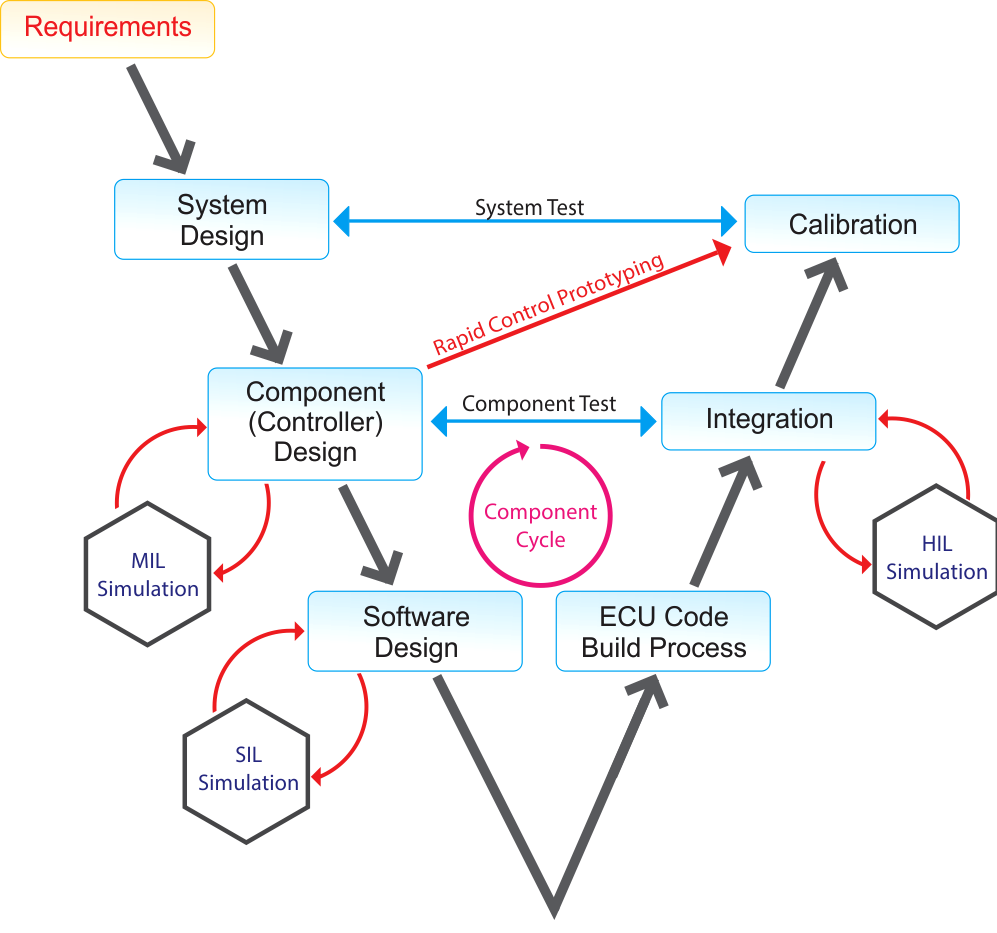
\includegraphics[width=10cm]{../Figures/QuadSimulation/ModelBasedDesign.png}
%	\centering
%	\caption{دیاگرام V 
%		\cite{Vdiagram}}
%	\label{Vdiag}
%\end{figure}
%\section{شبیه‌سازی استند سه درجه آزادی در محیط سیمولینک}\label{quadall3}
در این بخش به بررسی و شبیه‌سازی مدل دینامیکی استند سه درجه آزادی پرداخته شده است. در بخش \ref{spacestate} فرم فضای حالت استند چهارپره استخراج شد. در شبیه‌سازی نیز از همین روابط استخراج شده، استفاده شده است. مدل شبیه‌سازی شده از استند (شکل \ref{quadsimulink}) دارای چهار ورودی سرعت دورانی موتورها  و دارای سه خروجی زوایای رول ($\phi$)، پیچ ($\theta$)، یاو ($\psi$) و  سه سرعت زاویه‌ای
 \lr{p},
\lr{q}
 و 
\lr{r} 
 است.
 
 
\begin{figure}[H]
	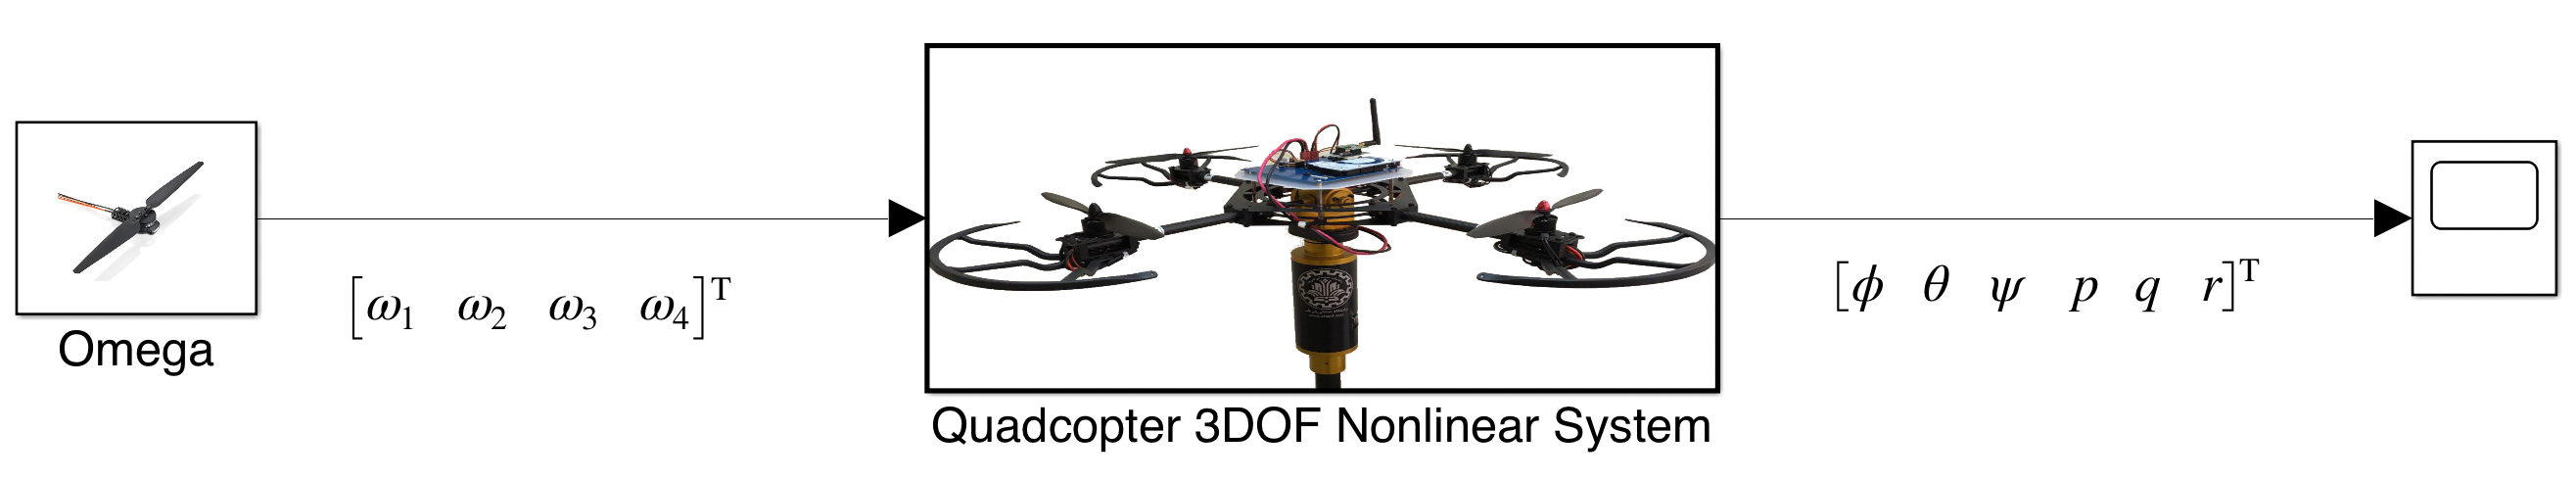
\includegraphics[width=16cm]{../Figures/QuadSimulation/Stand_Model.png}
	\centering
	\vspace*{-15mm}
	\caption{مدل استند چهارپره شبیه‌سازی شده در سیمولینک و نمایش ورودی و خروجی‌های مدل}
	\label{quadsimulink}
\end{figure}
نمایی از داخل بلوک
\lr{Quacopter 3DOF Nonlinear System}
در شکل \ref{Quad3DOF} آورده شده است.
%\newline
%\newline
\begin{figure}[H]
	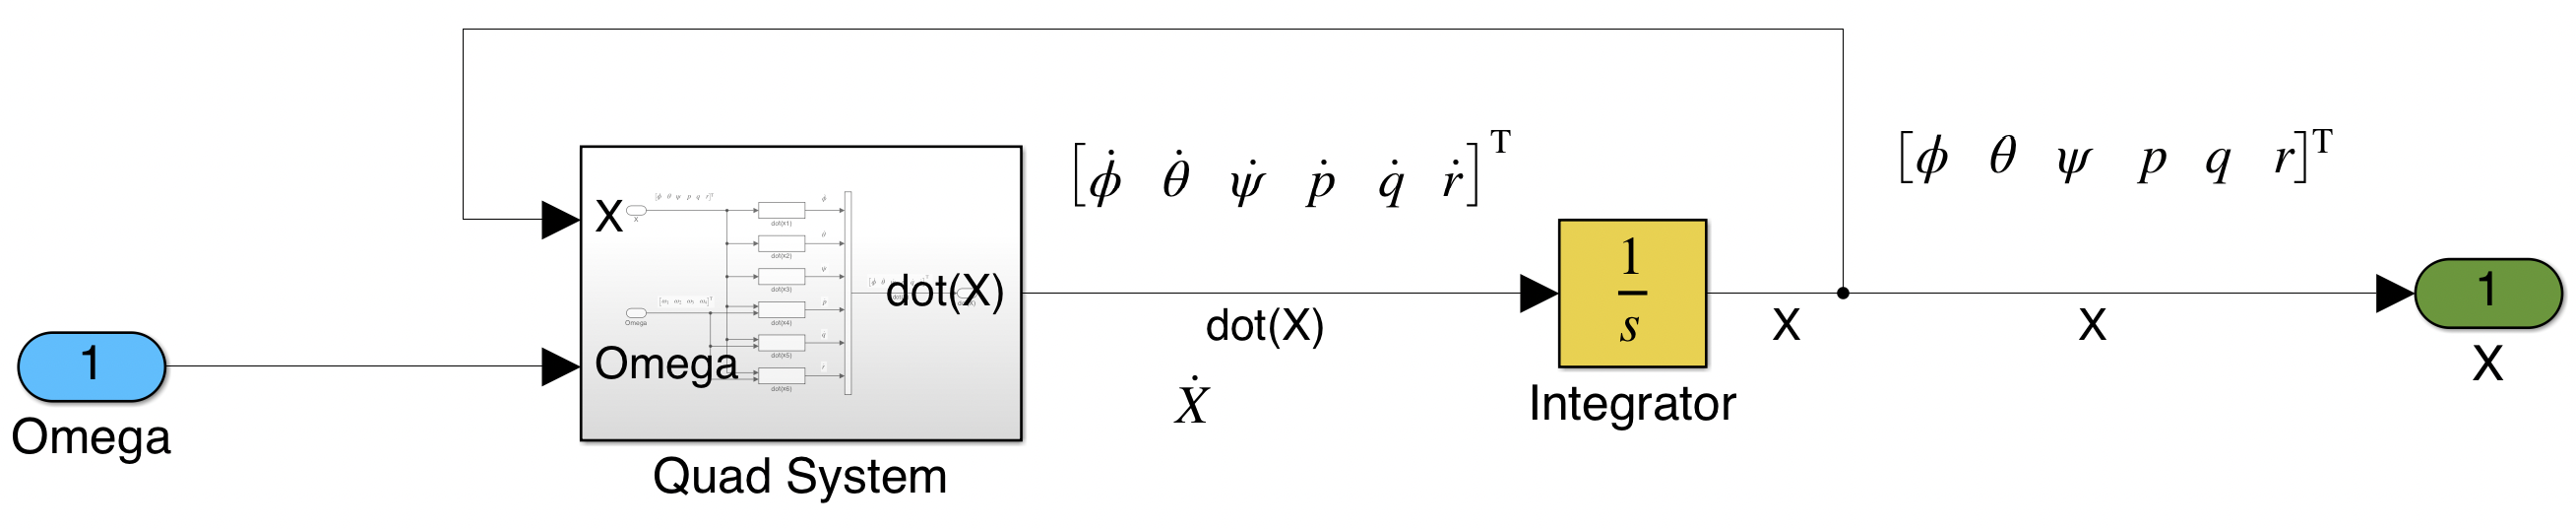
\includegraphics[width=16cm]{../Figures/QuadSimulation/Integrator.png}
	\centering
	\vspace*{-15mm}
	\caption{مدل استند چهارپره شبیه‌سازی شده در سیمولینک و نمایش ورودی و خروجی‌های مدل}
	\label{Quad3DOF}
\end{figure}
خروجی بلوک
\lr{Quad System}،
$\dot X$
است. با استفاده از بلوک انتگرال‌گیر (بلوک زرد رنگ در شکل \ref{Quad3DOF})
از خروجی بلوک بر اساس شرایط اولیه استند انتگرال گرفته می‌شود و وضعیت استند (زاویه‌های رول ($\phi$)، پیچ ($\theta$)، یاو ($\psi$) و سرعت‌های زاویه‌ای‌
 \lr{p},
\lr{q}
و 
\lr{r})
را خروجی می‌دهد.

در داخل بلوک
\lr{Quad System}،
شش بلوک دیگر قرار دارد که تعدادی از آن‌ها دارای ورودی $X$ و تعدادی دیگر دارای ورودی $X$ و $\omega$ هستند. مجموع خروجی این شش بلوک $\dot X$ است که در توضیحات بلوک
\lr{Quad System}،
 نیز به آن اشاره شد.
نمایی از داخل بلوک
\lr{Quad System}
در شکل \ref{all-six} آورده شده است.
\begin{figure}[H]
	\includegraphics[width=16cm]{../Figures/QuadSimulation/all-six.png}
	\centering
%	\vspace*{-15mm}
	\caption{نمایی از داخل بلوک \lr{Quad System}}
	\label{all-six}
\end{figure}
%\section{شبیه‌سازی کانال‌های مختلف استند سه درجه آزادی در محیط سیمولینک}
 در بخش
(\ref{quadall3})
 به شبیه‌سازی سه درجه آزادی استند چهارپره پرداخته شد. در این بخش به شبیه‌سازی کانال‌های رول، پیج، یاو و رول-پیچ پرداخته می‌شود. برای شبیه‌سازی یک کانال فرض شده است سایر کانال‌ها بسته شده‌اند و هیچگونه حرکتی در این کانال‌ها وجود ندارد.
 
\subsection{شبیه سازی کانال رول در محیط سیمولینک}
در بخش
\ref{lin_SISO}
فرم فضای حالت کانال‌های مختلف استند چهار پره بدست آمد در این بخش فرم فضای حالت کانال رول در سیمولینک شبیه‌سازی می‌شود.
مدل شبیه‌سازی شده از استند (شکل \ref{roll_simulink}) دارای دو ورودی سرعت دورانی موتورهای دو و چهار  و دارای یک خروجی زاویه‌ی رول ($\phi$) و  سرعت زاویه‌ای p است.
\begin{figure}[H]
	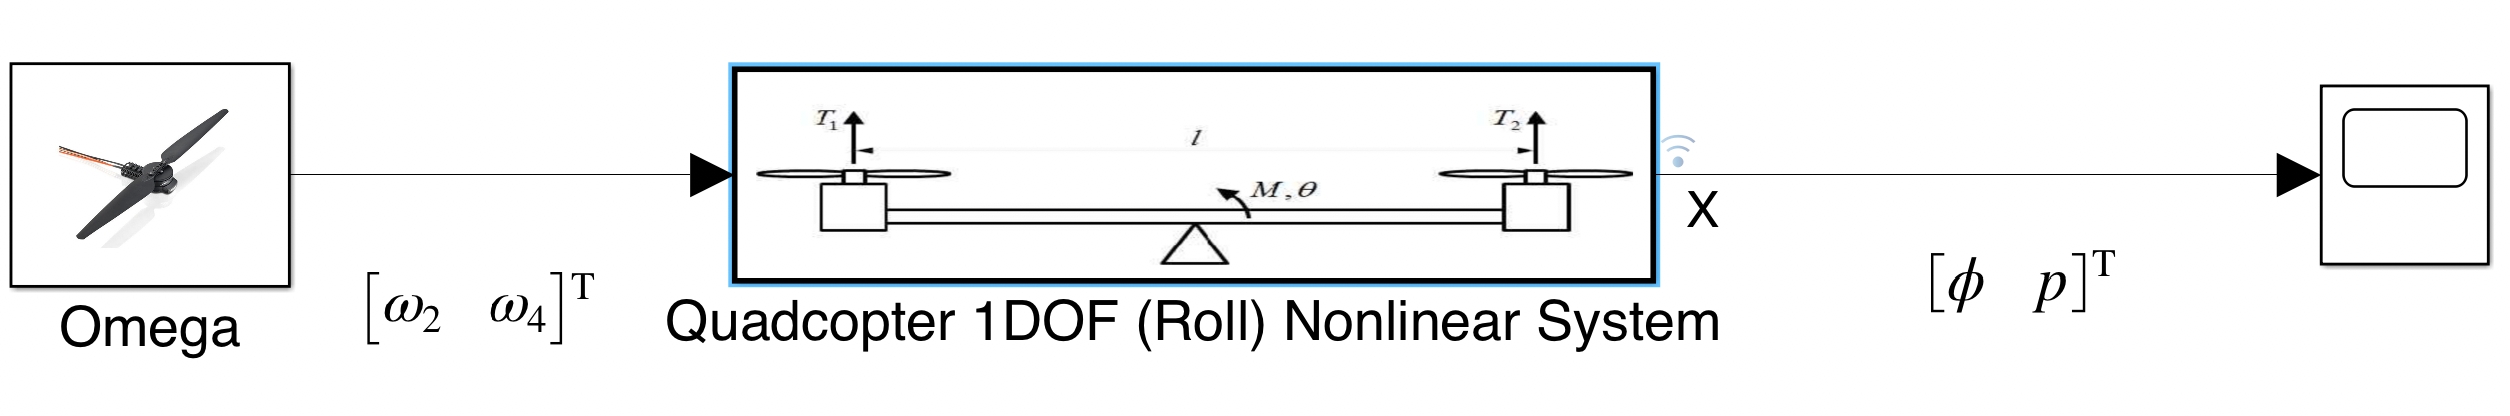
\includegraphics[width=16cm]{../../Figures/QuadSimulation/roll_Stand_Model.png}
	\centering
	\vspace*{-15mm}
	\caption{مدل کانال رول استند چهارپره شبیه‌سازی شده در سیمولینک و نمایش ورودی و خروجی‌ها}
	\label{roll_simulink}
\end{figure}

نمایی از داخل بلوک
\lr{Quacopter 1DOF (Roll) Nonlinear System}
در شکل (\ref{Quad1DOF_roll}) آورده شده است.
%\newline
%\newline
\begin{figure}[H]
	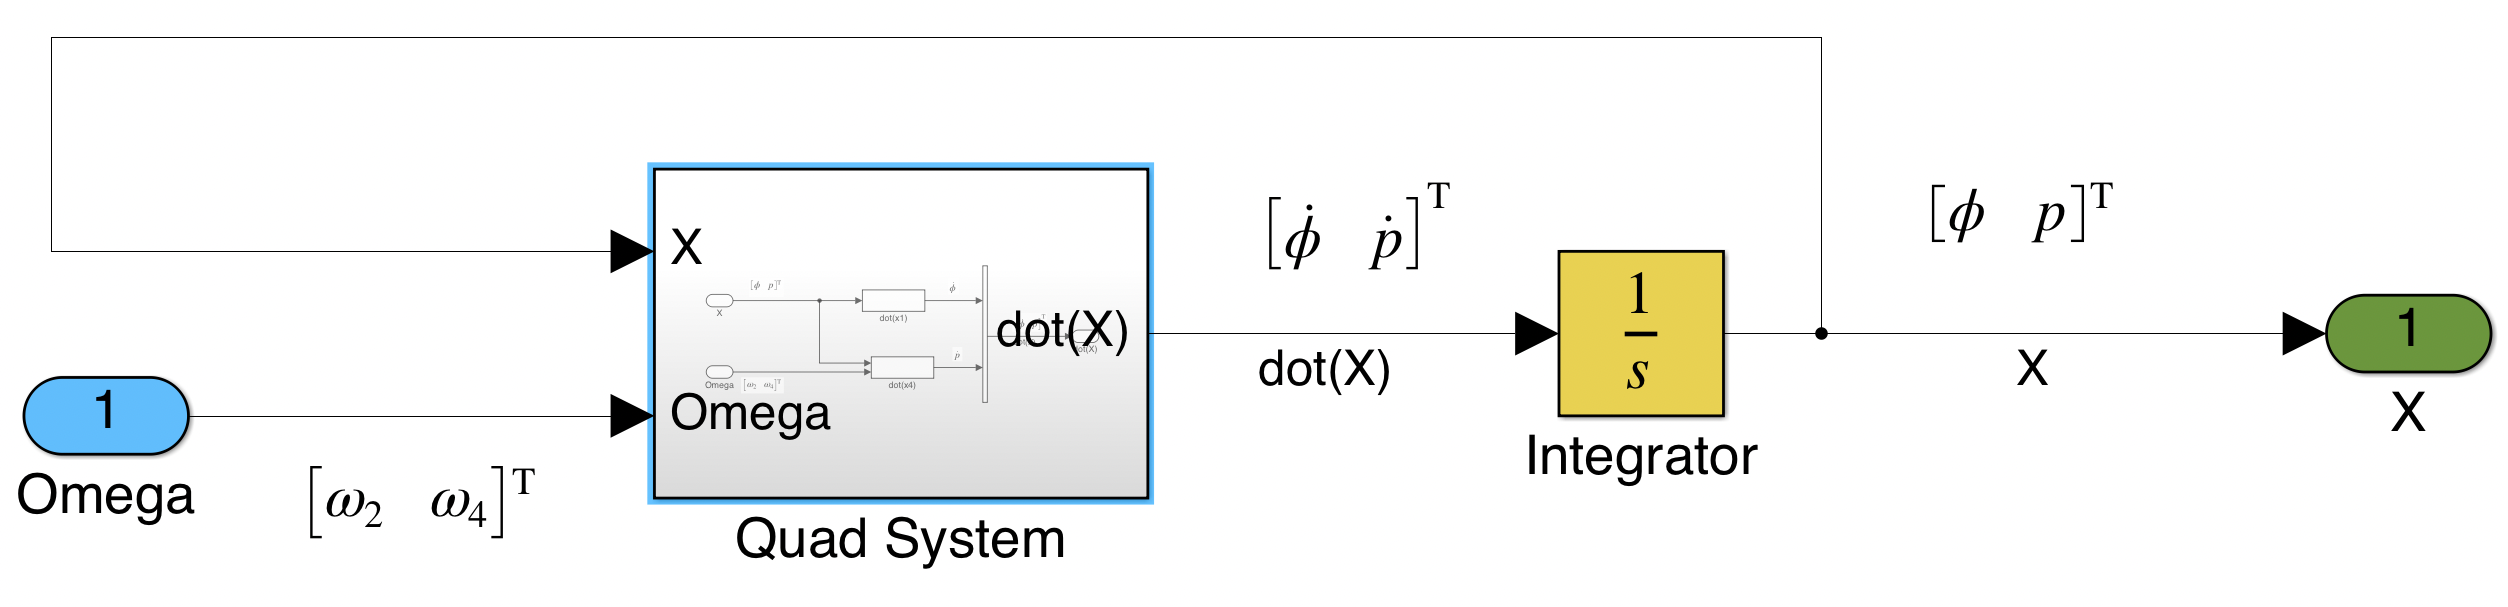
\includegraphics[width=16cm]{../../Figures/QuadSimulation/roll_Integrator.png}
	\centering
	\vspace*{-15mm}
	\caption{مدل کانال رول استند چهارپره شبیه‌سازی شده در سیمولینک و نمایش ورودی و خروجی‌ها}
	\label{Quad1DOF_roll}
\end{figure}
بلوک
\lr{Quad System}،
$\dot X$ را به عنوان خروجی می‌دهد. با استفاده از بلوک انتگرالگیر (بلوک زرد رنگ) در شکل
(\ref{Quad3DOF})
از خروجی آن بر اساس شرایط اولیه استند انتگرال گرفته می‌شود و خروجی مورد نیاز ( زاویه رول ($\phi$) و سرعت زاویه‌ای‌
p)
را می دهد.

داخل بلوک
\lr{Quad System}،
دو بلوک دارد که یکی از آن‌های دارای ورودی $X$ و دیگری دارای ورودی $X$ و $\omega$ هستند. مجموع خروحی این دو بلوک $\dot X$ است که برای بلوک
\lr{Quad System}،
نیز اشاره شد.
نمایی از داخل بلوک
\lr{Quad System}
در شکل (\ref{roll_all-six}) آورده شده است.
\begin{figure}[H]
	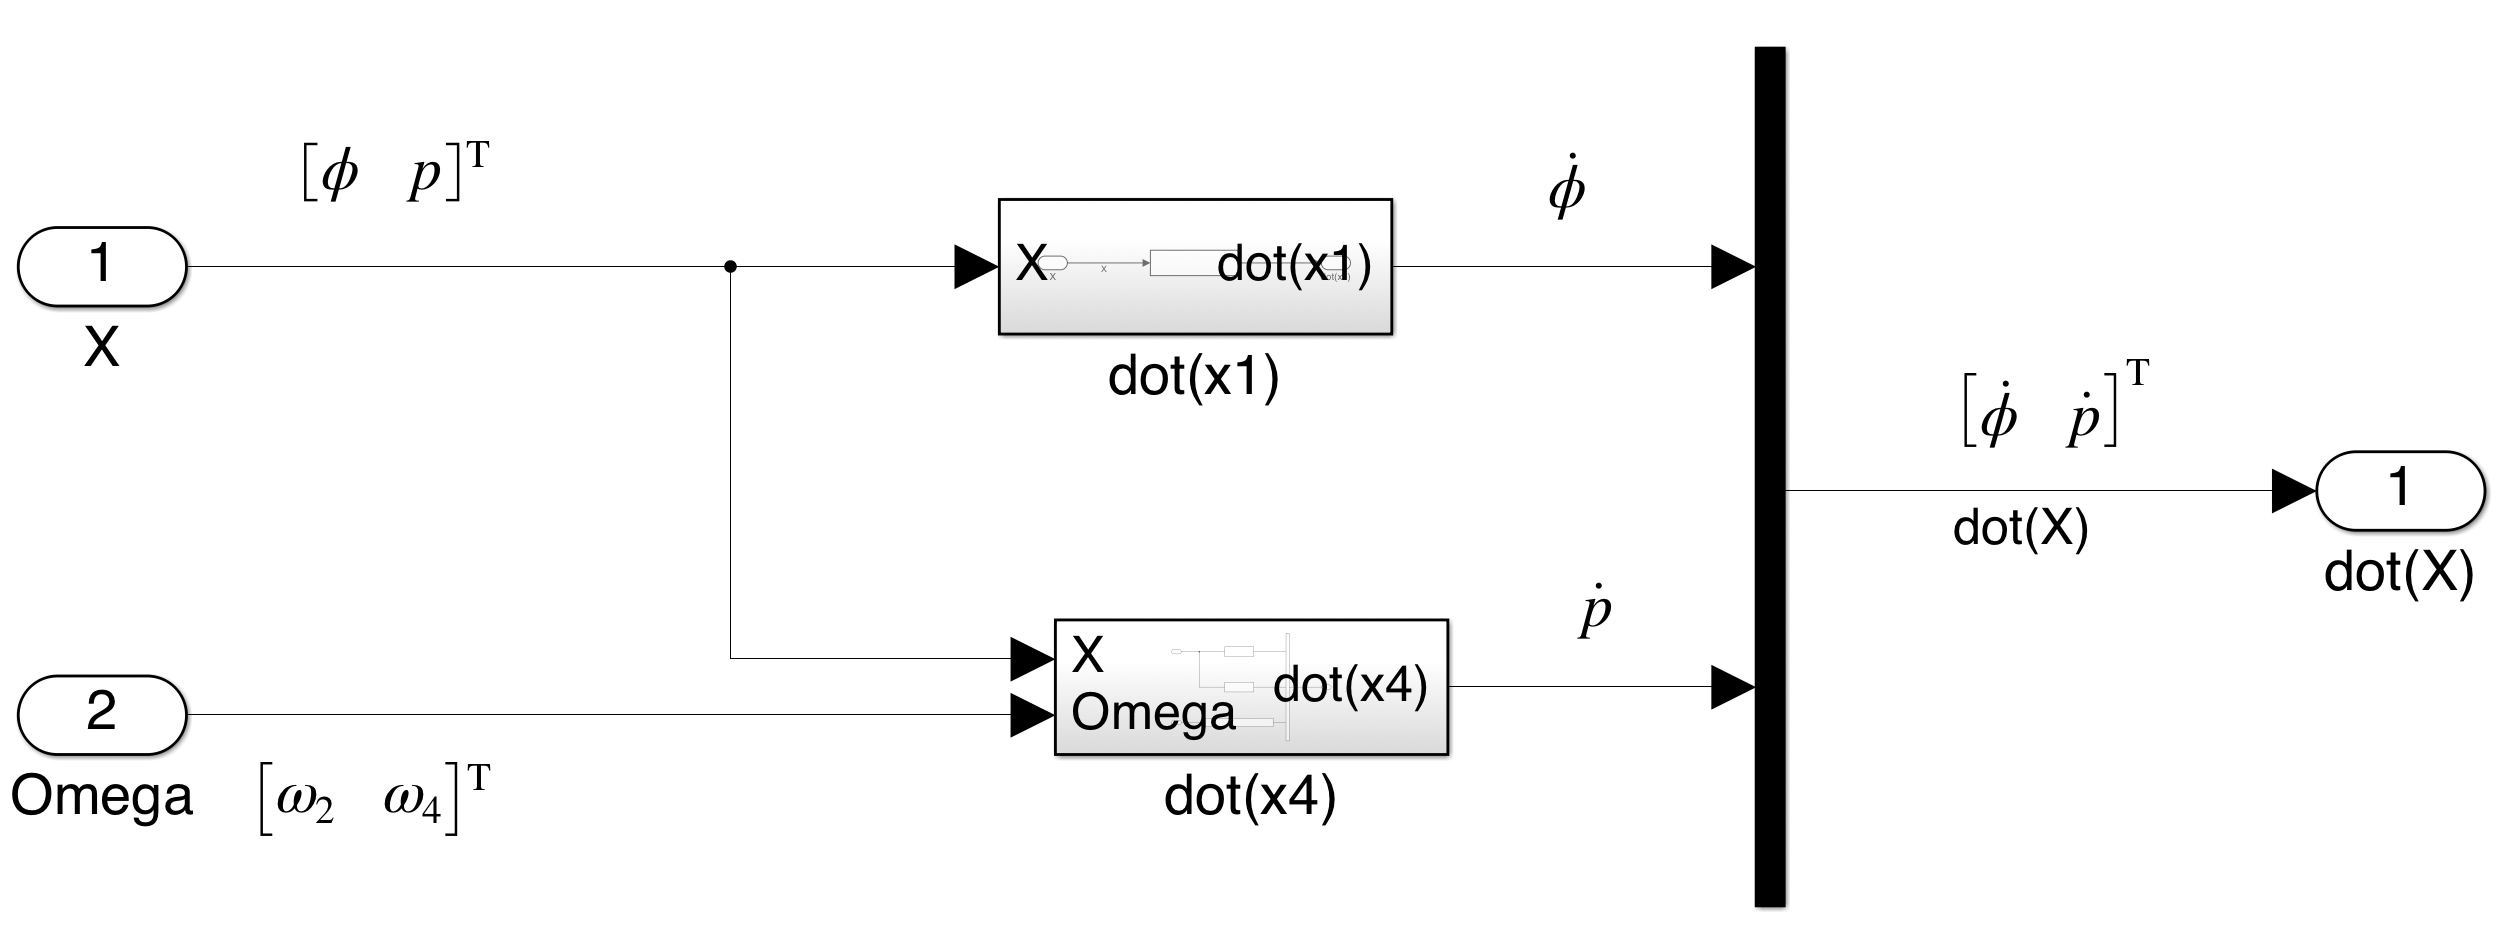
\includegraphics[width=16cm]{../../Figures/QuadSimulation/roll_all-six.png}
	\centering
	%	\vspace*{-15mm}
	\caption{نمایی از داخل بلوک \lr{Quad System}}
	\label{roll_all-six}
\end{figure}

\subsection{شبیه سازی کانال پیچ در محیط سیمولینک}
در بخش
\ref{lin_SISO}
فرم فضای حالت کانال‌های مختلف استند چهار پره بدست آمد در این بخش فرم فضای حالت کانال پیچ در سیمولینک شبیه‌سازی می‌شود.
مدل شبیه‌سازی شده از استند (شکل \ref{pitch_simulink}) دارای دو ورودی سرعت دورانی موتورهای یک و سه  و دارای یک خروجی زاویه‌ی پیچ ($\theta$) و  سرعت زاویه‌ای q است.
\begin{figure}[H]
	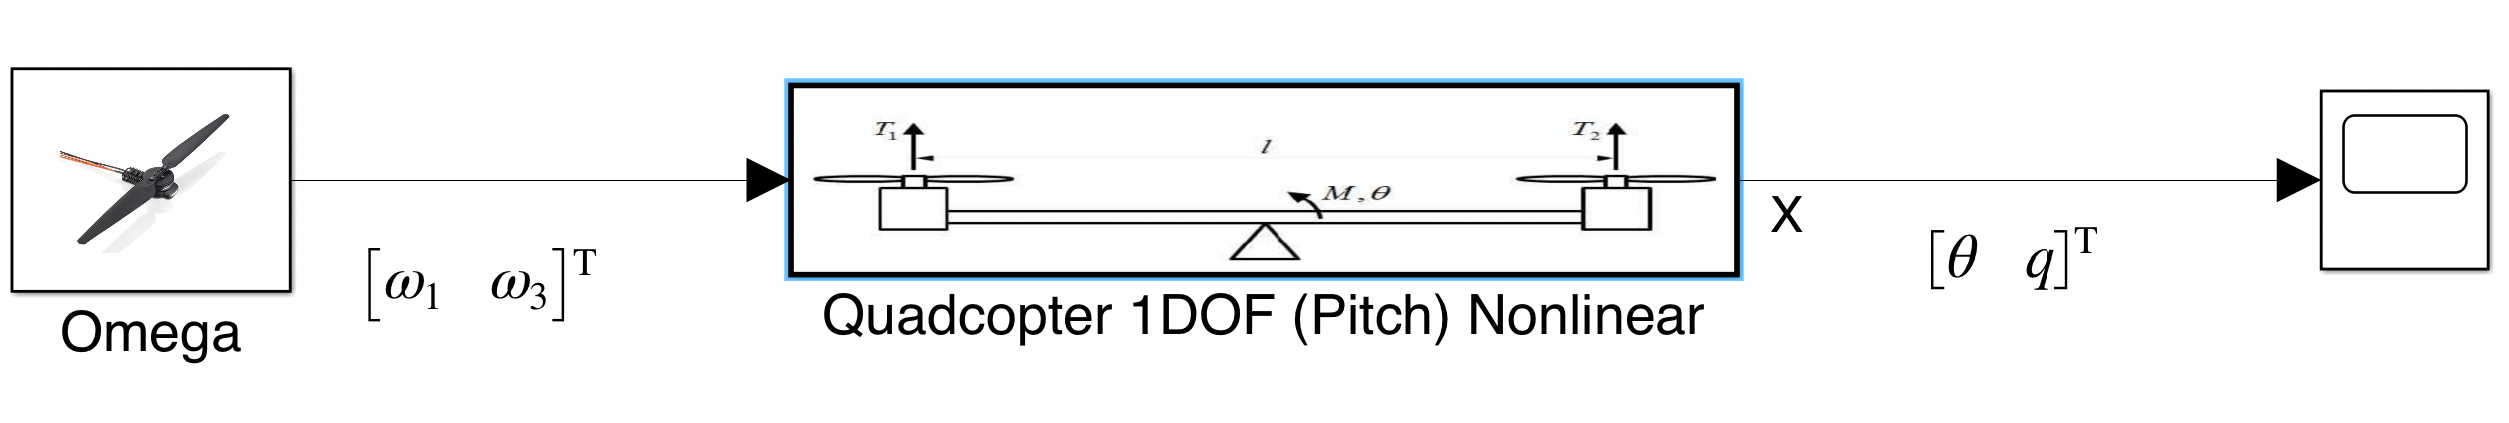
\includegraphics[width=16cm]{../../Figures/QuadSimulation/pitch_Stand_Model.png}
	\centering
	\vspace*{-15mm}
	\caption{مدل کانال رول استند چهارپره شبیه‌سازی شده در سیمولینک و نمایش ورودی و خروجی‌ها}
	\label{pitch_simulink}
\end{figure}

نمایی از داخل بلوک
\lr{Quacopter 1DOF (Pitch) Nonlinear System}
در شکل (\ref{Quad1DOF_pitch}) آورده شده است.
%\newline
%\newline
\begin{figure}[H]
	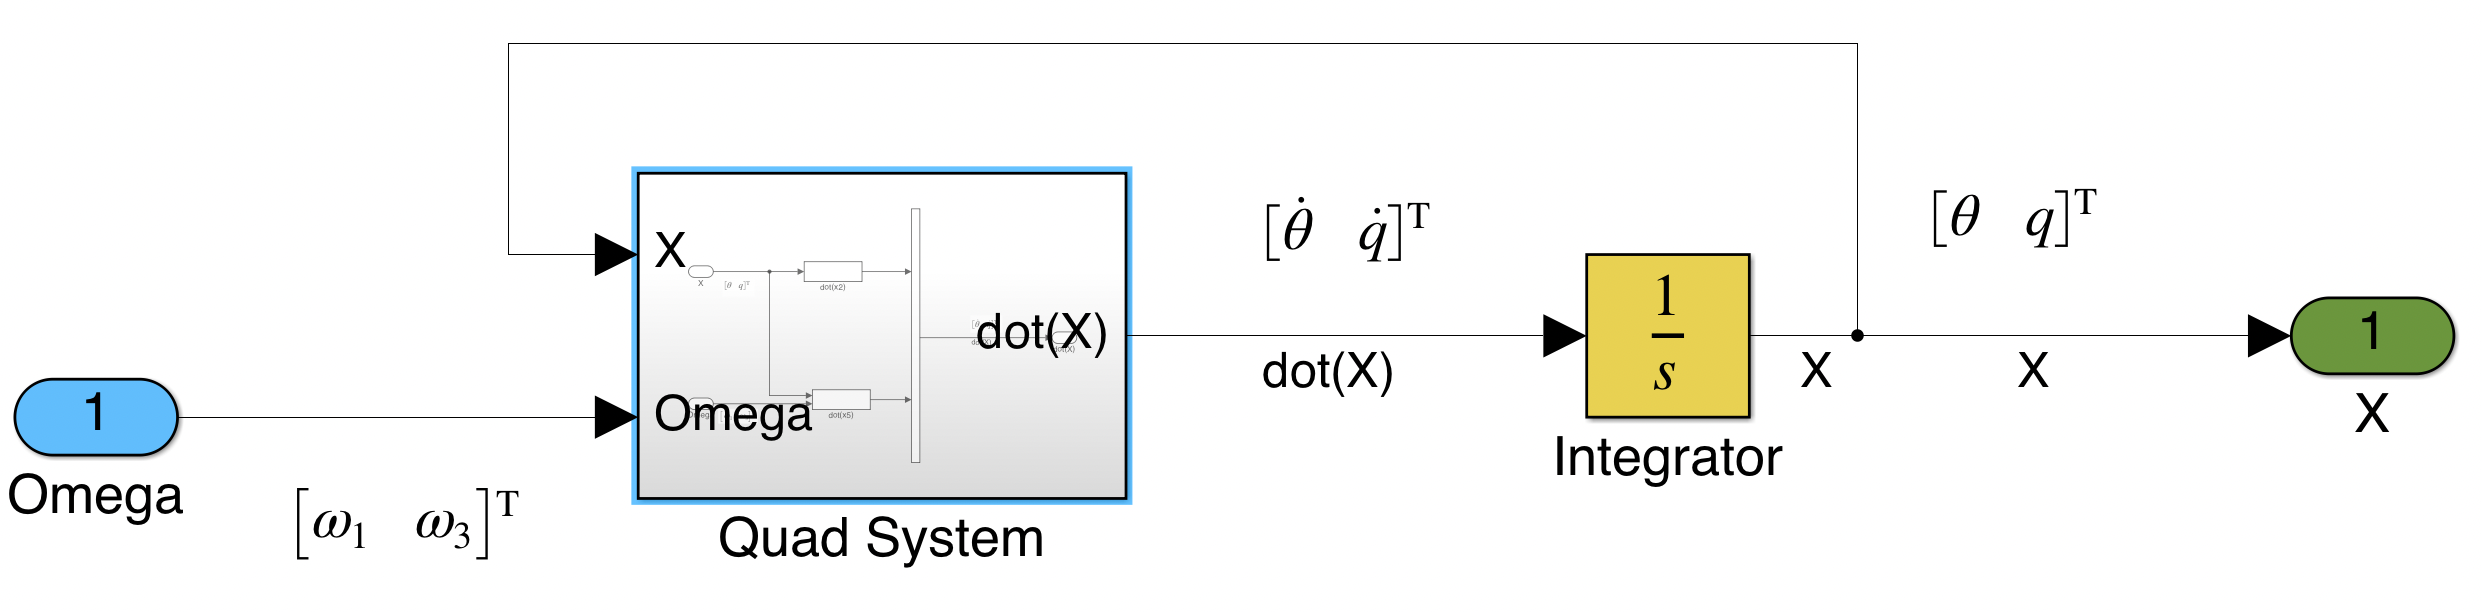
\includegraphics[width=16cm]{../../Figures/QuadSimulation/pitch_Integrator.png}
	\centering
	\vspace*{-15mm}
	\caption{مدل کانال رول استند چهارپره شبیه‌سازی شده در سیمولینک و نمایش ورودی و خروجی‌ها}
	\label{Quad1DOF_pitch}
\end{figure}
بلوک
\lr{Quad System}،
$\dot X$ را به عنوان خروجی می‌دهد. با استفاده از بلوک انتگرالگیر (بلوک زرد رنگ) در شکل
(\ref{Quad3DOF})
از خروجی آن بر اساس شرایط اولیه استند انتگرال گرفته می‌شود و خروجی مورد نیاز ( زاویه پیچ ($\theta$) و سرعت زاویه‌ای‌
q)
را می دهد.

داخل بلوک
\lr{Quad System}،
دو بلوک دارد که یکی از آن‌های دارای ورودی $X$ و دیگری دارای ورودی $X$ و $\omega$ هستند. مجموع خروحی این دو بلوک $\dot X$ است که برای بلوک
\lr{Quad System}،
نیز اشاره شد.
نمایی از داخل بلوک
\lr{Quad System}
در شکل (\ref{pitch_all-six}) آورده شده است.
\begin{figure}[H]
	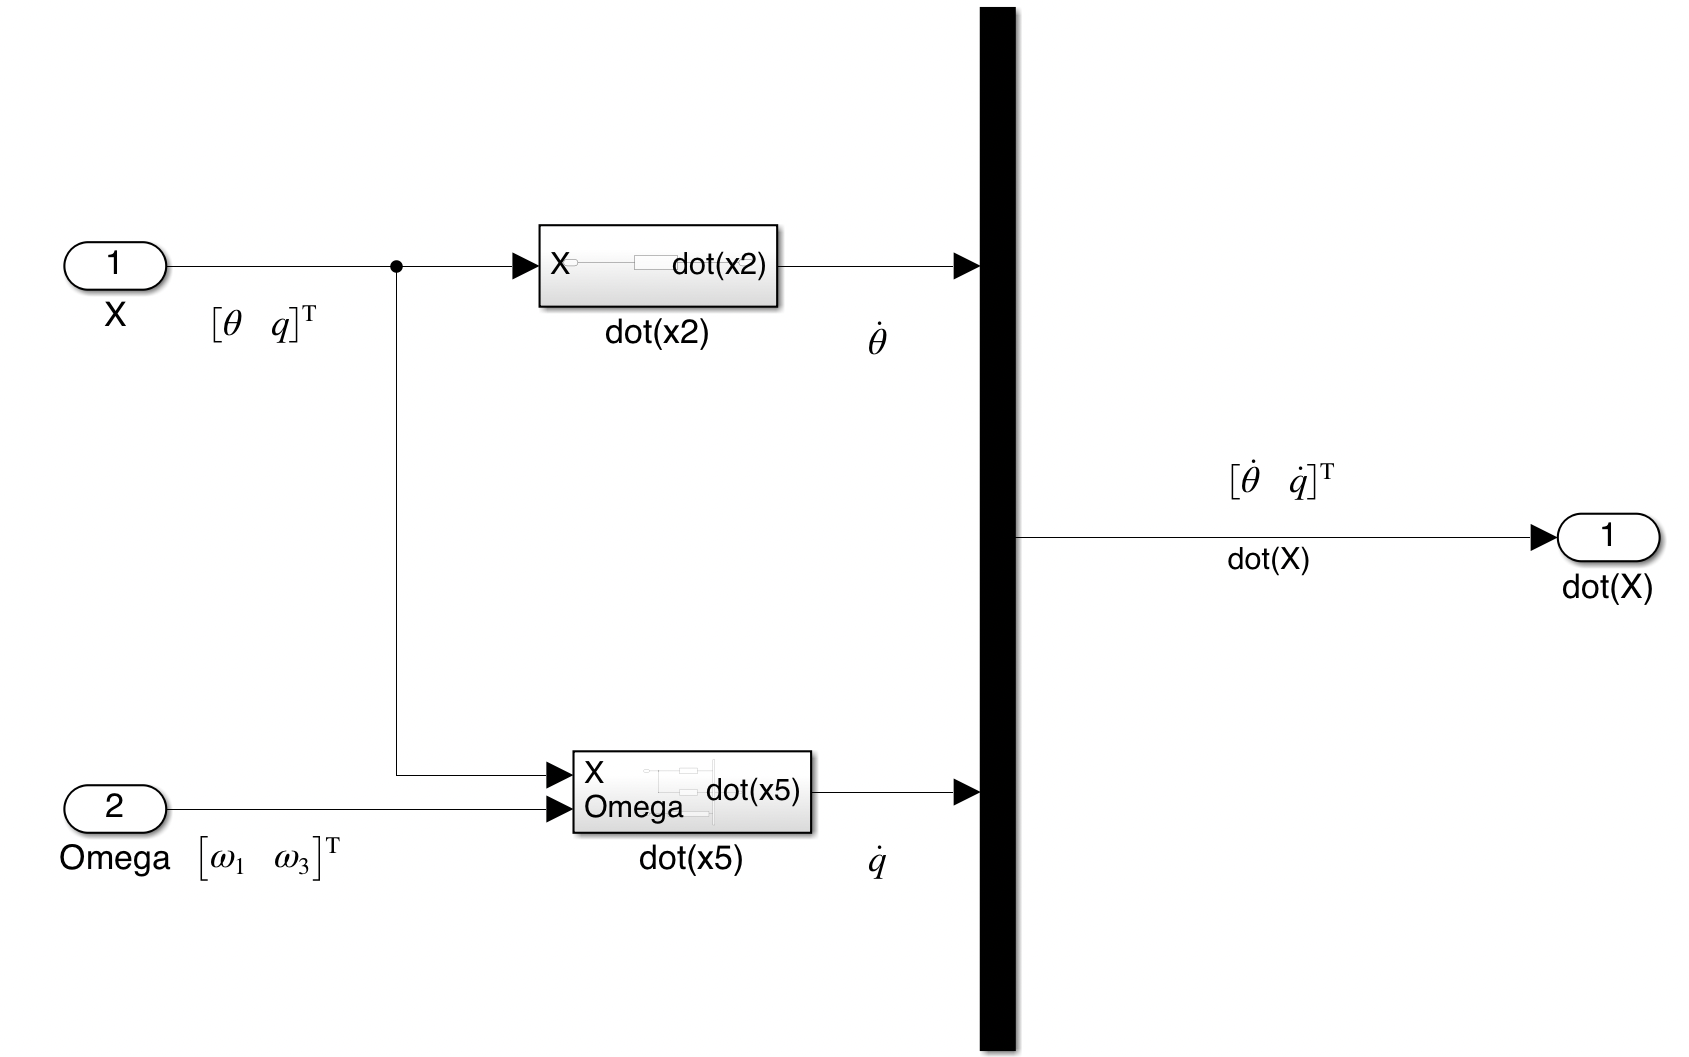
\includegraphics[width=16cm]{../../Figures/QuadSimulation/pitch_all-six.png}
	\centering
	%	\vspace*{-15mm}
	\caption{نمایی از داخل بلوک \lr{Quad System}}
	\label{pitch_all-six}
\end{figure}

\subsection{شبیه سازی کانال یاو در محیط سیمولینک}
در بخش
\ref{lin_SISO}
فرم فضای حالت کانال‌های مختلف استند چهار پره بدست آمد در این بخش فرم فضای حالت کانال رول در سیمولینک شبیه‌سازی می‌شود.
مدل شبیه‌سازی شده از استند (شکل \ref{yaw_simulink}) دارای چهار ورودی سرعت دورانی موتورها  و دارای یک خروجی زاویه‌ی رول ($\psi$) و  سرعت زاویه‌ای r است.
\begin{figure}[H]
	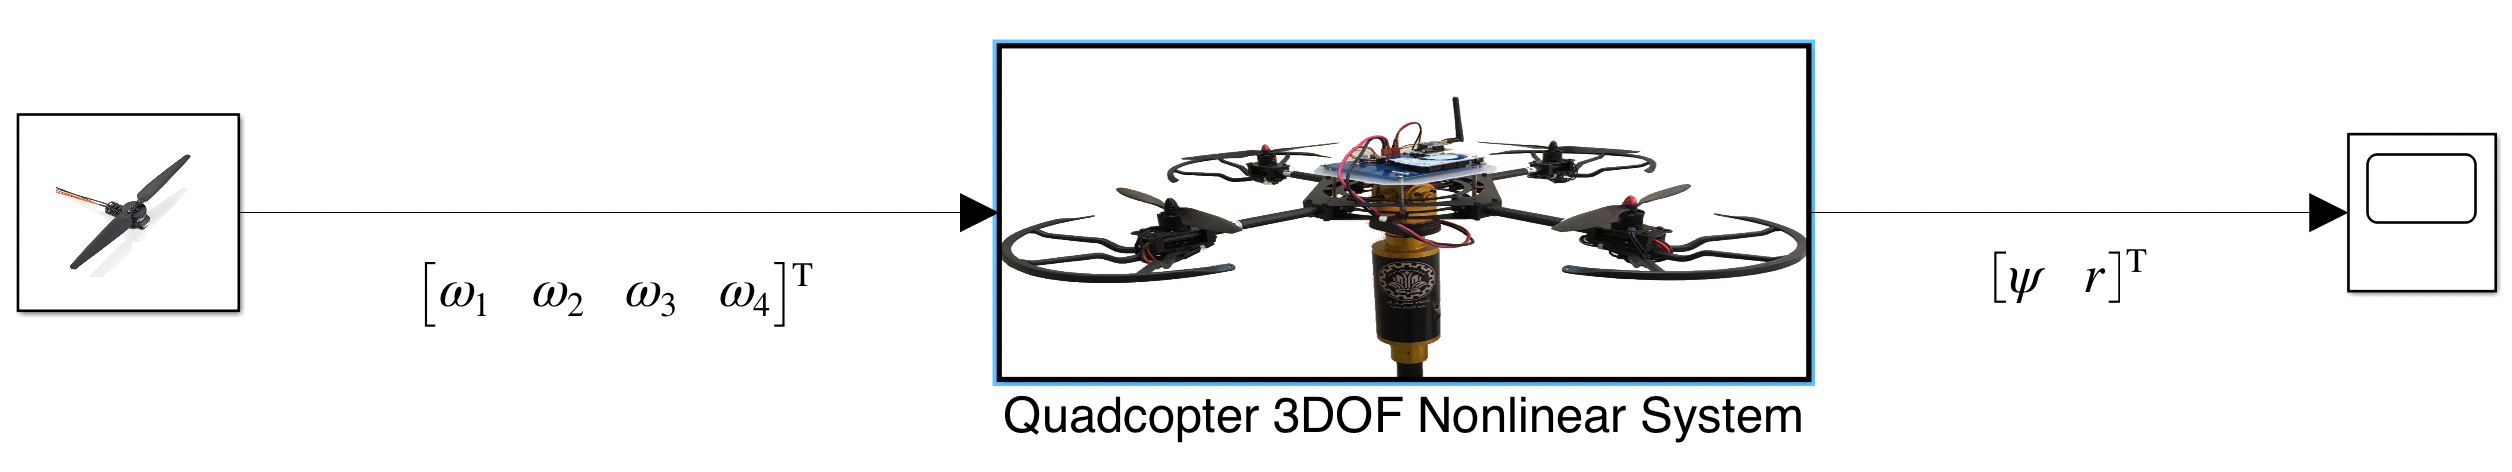
\includegraphics[width=16cm]{../../Figures/QuadSimulation/yaw_Stand_Model.png}
	\centering
	\vspace*{-15mm}
	\caption{مدل کانال رول استند چهارپره شبیه‌سازی شده در سیمولینک و نمایش ورودی و خروجی‌ها}
	\label{yaw_simulink}
\end{figure}

نمایی از داخل بلوک
\lr{Quacopter 1DOF (Yaw) Nonlinear System}
در شکل (\ref{Quad1DOF_yaw}) آورده شده است.
%\newline
%\newline
\begin{figure}[H]
	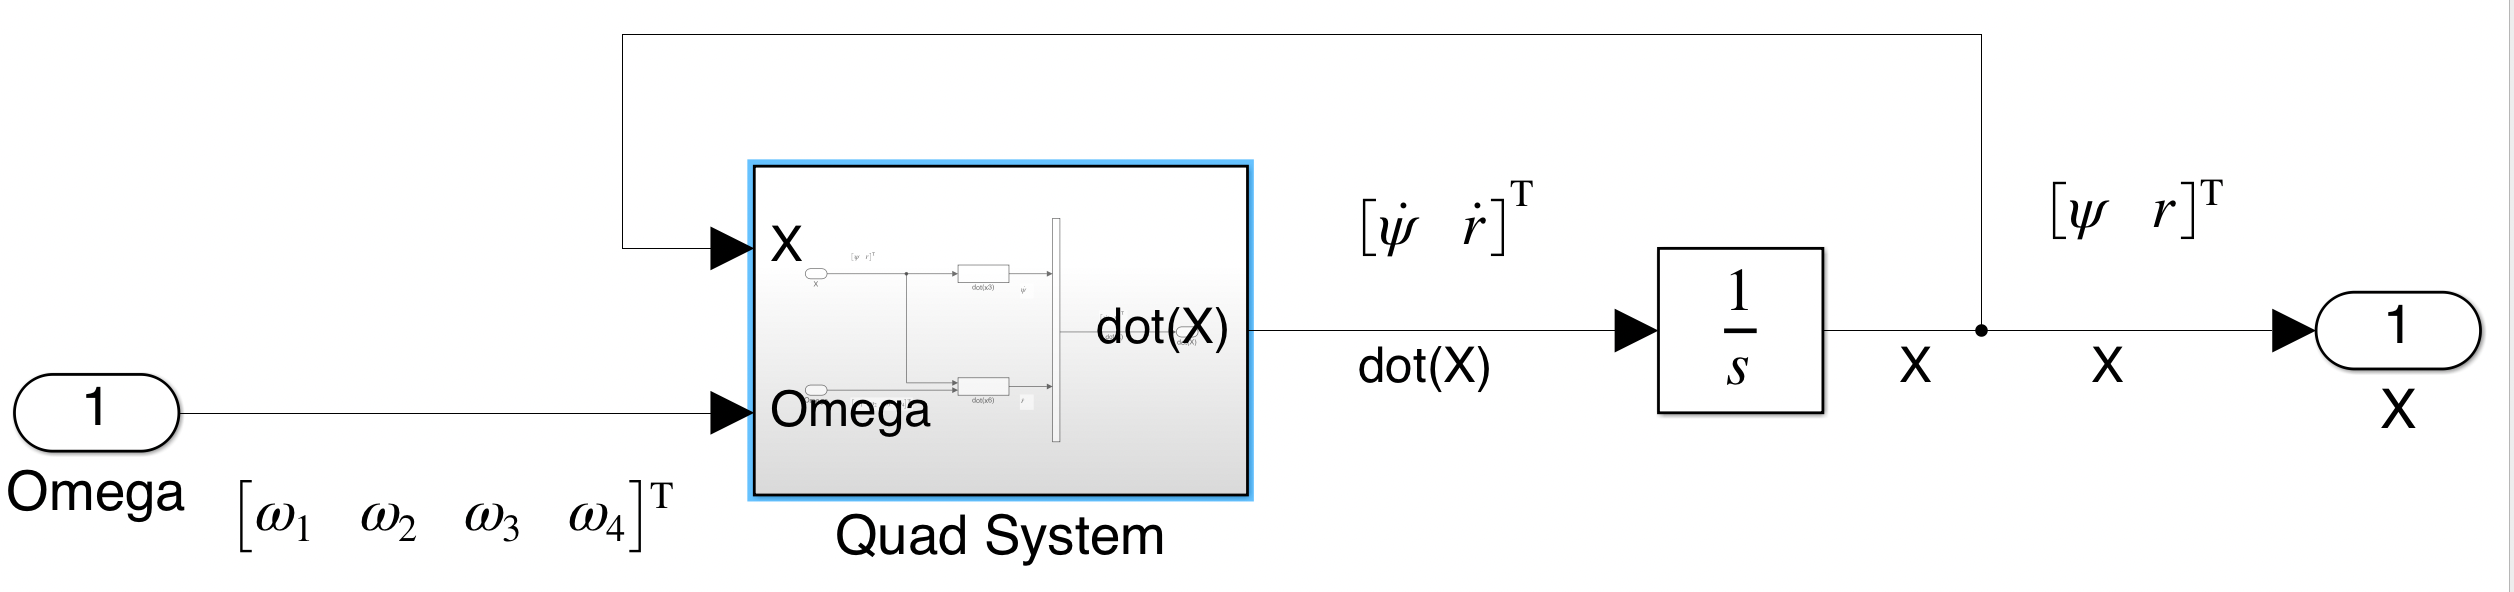
\includegraphics[width=16cm]{../../Figures/QuadSimulation/yaw_Integrator.png}
	\centering
	\vspace*{-15mm}
	\caption{مدل کانال یاو استند چهارپره شبیه‌سازی شده در سیمولینک و نمایش ورودی و خروجی‌ها}
	\label{Quad1DOF_yaw}
\end{figure}
بلوک
\lr{Quad System}،
$\dot X$ را به عنوان خروجی می‌دهد. با استفاده از بلوک انتگرالگیر (بلوک زرد رنگ) در شکل
(\ref{Quad3DOF})
از خروجی آن بر اساس شرایط اولیه استند انتگرال گرفته می‌شود و خروجی مورد نیاز ( زاویه‌های یاو ($\psi$) و سرعت زاویه‌ای‌
q)
را می دهد.

داخل بلوک
\lr{Quad System}،
دو بلوک دارد که یکی از آن‌های دارای ورودی $X$ و دیگری دارای ورودی $X$ و $\omega$ هستند. مجموع خروحی این دو بلوک $\dot X$ است که برای بلوک
\lr{Quad System}،
نیز اشاره شد.
نمایی از داخل بلوک
\lr{Quad System}
در شکل (\ref{yaw_all-six}) آورده شده است.
\begin{figure}[H]
	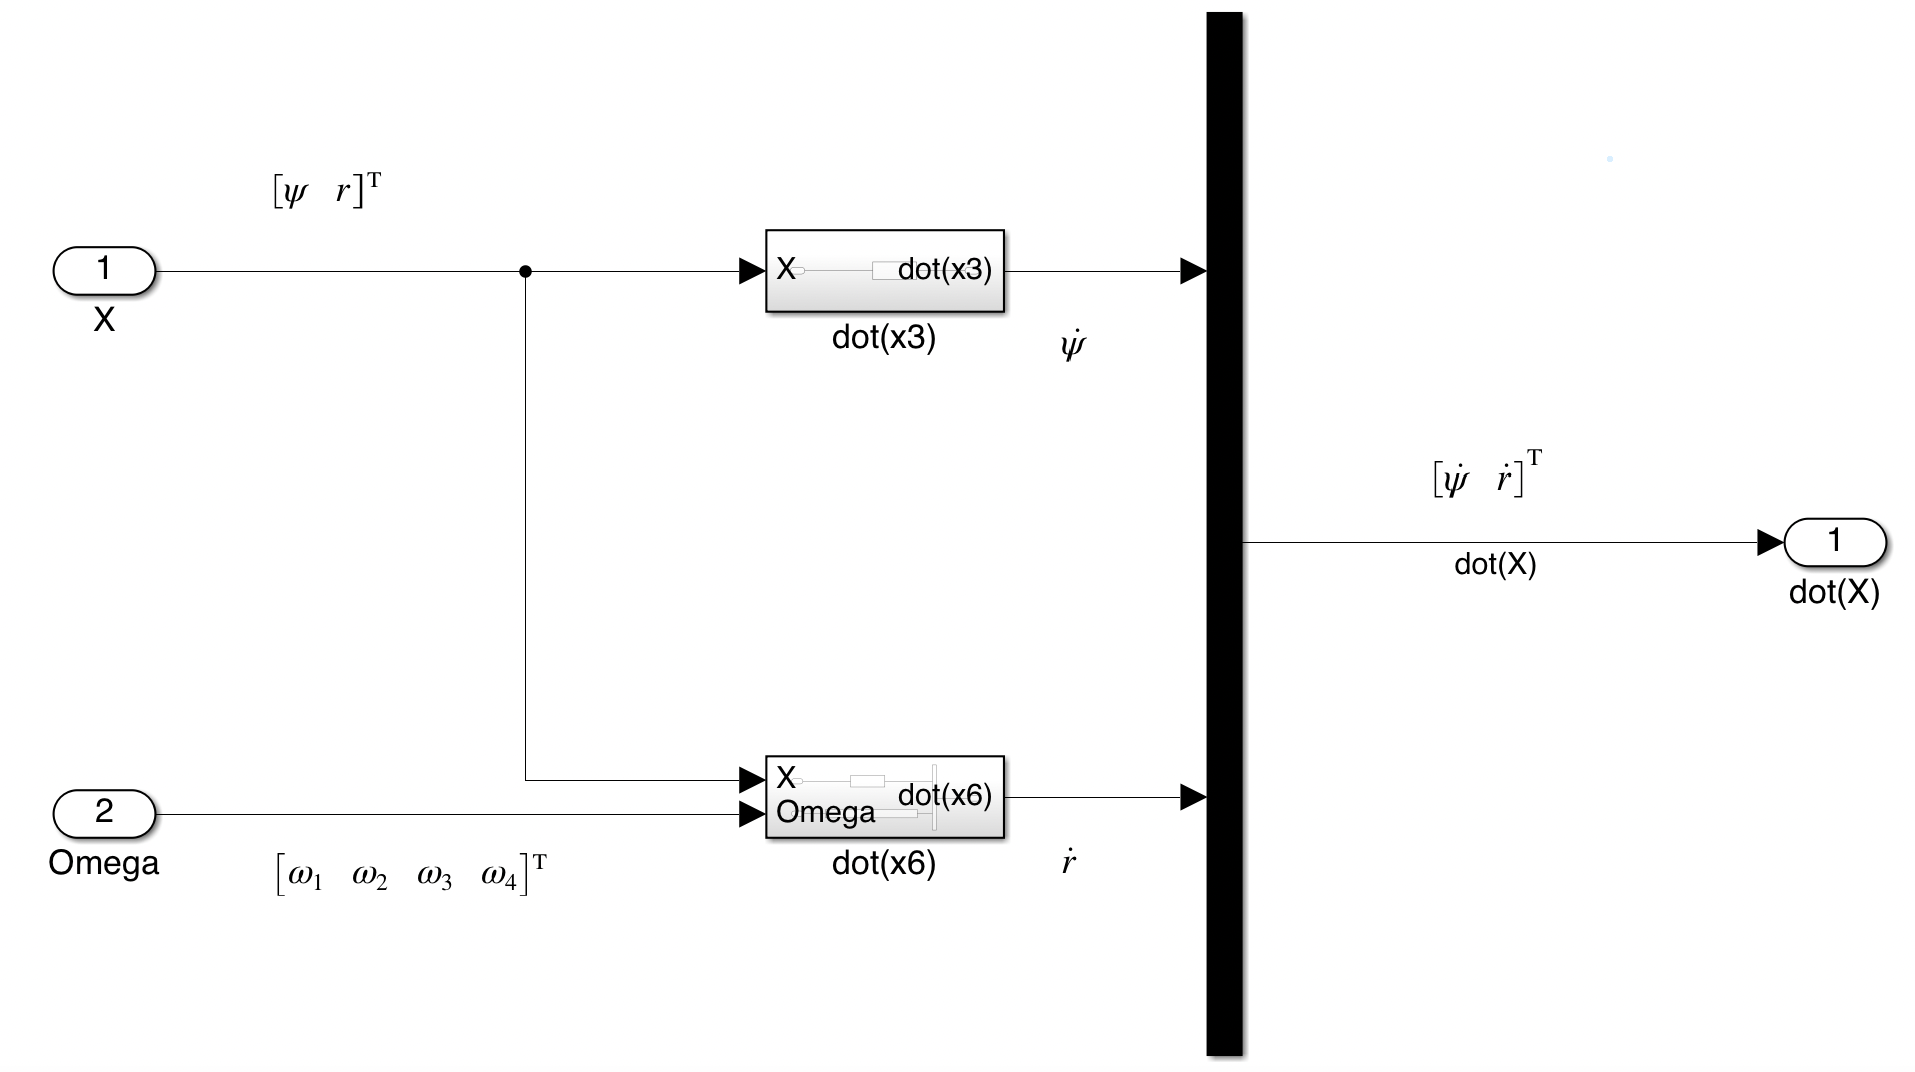
\includegraphics[width=16cm]{../../Figures/QuadSimulation/yaw_all-six.png}
	\centering
	%	\vspace*{-15mm}
	\caption{نمایی از داخل بلوک \lr{Quad System}}
	\label{yaw_all-six}
\end{figure}
%\section{اصلاح پارامتر‌های  استند چهارپره}\label{parameeter_estimation_section}
در بخش
\ref{spacestate}
فرم فضای حالت استند چهارپره استخراج شد و  در بخش
\ref{quadall3}
شبیه‌سازی استند چهارپره انجام شد.
در این بخش، با استفاده از شبیه‌سازی کانال‌های مختلف چهارپره در محیط سیمولینک و داده‌های خروجی  از استند چهارپره، پارامترهای استند چهارپره اصلاح می‌شوند.

برای اصلاح پارامترهای استند چهارپره از جعبه‌ابزار
\lr{Parameter Estimator}
موجود در محیط سیمولینک
استفاده شده‌است.
%این جعبه ابزار با استفاده از داده‌های وضعیت استند در واقعیت و داده‌های وضعیت استند در شبیه‌سازی سیمولینک، اقدام به اصلاح پارامترهای موجود در شبیه‌سازی می‌کند، به‌صورتی که وضعیت استند در شبیه‌سازی تا حد ممکن به  وضعیت استند در واقعیت نزدیک کند.
%
%%\newline
%
%	\hspace*{.5cm}
%\begin{figure}[H]
%
%	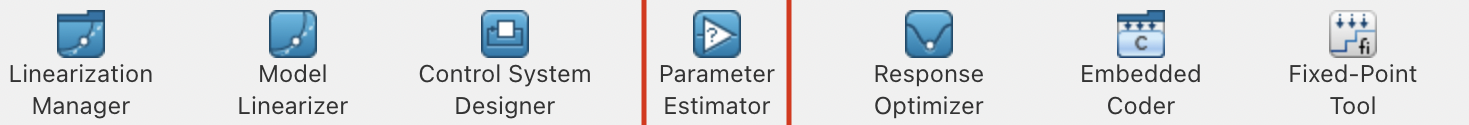
\includegraphics[width=12cm]{../Figures/QuadSimulation/ParameterEstimation/PS_icon.png}
%	\centering
%	\caption{نماد جعبه‌ابزار
%	\lr{Parameter Estimator}
%در سیمولینک}
%\end{figure}
%در شکل
%\ref{PS}
%نمایی از این جعبه‌ابزار آورده شده‌است.
%
%
%
%
%
%	\hspace*{-0.5cm}
%\begin{figure}[H]
%	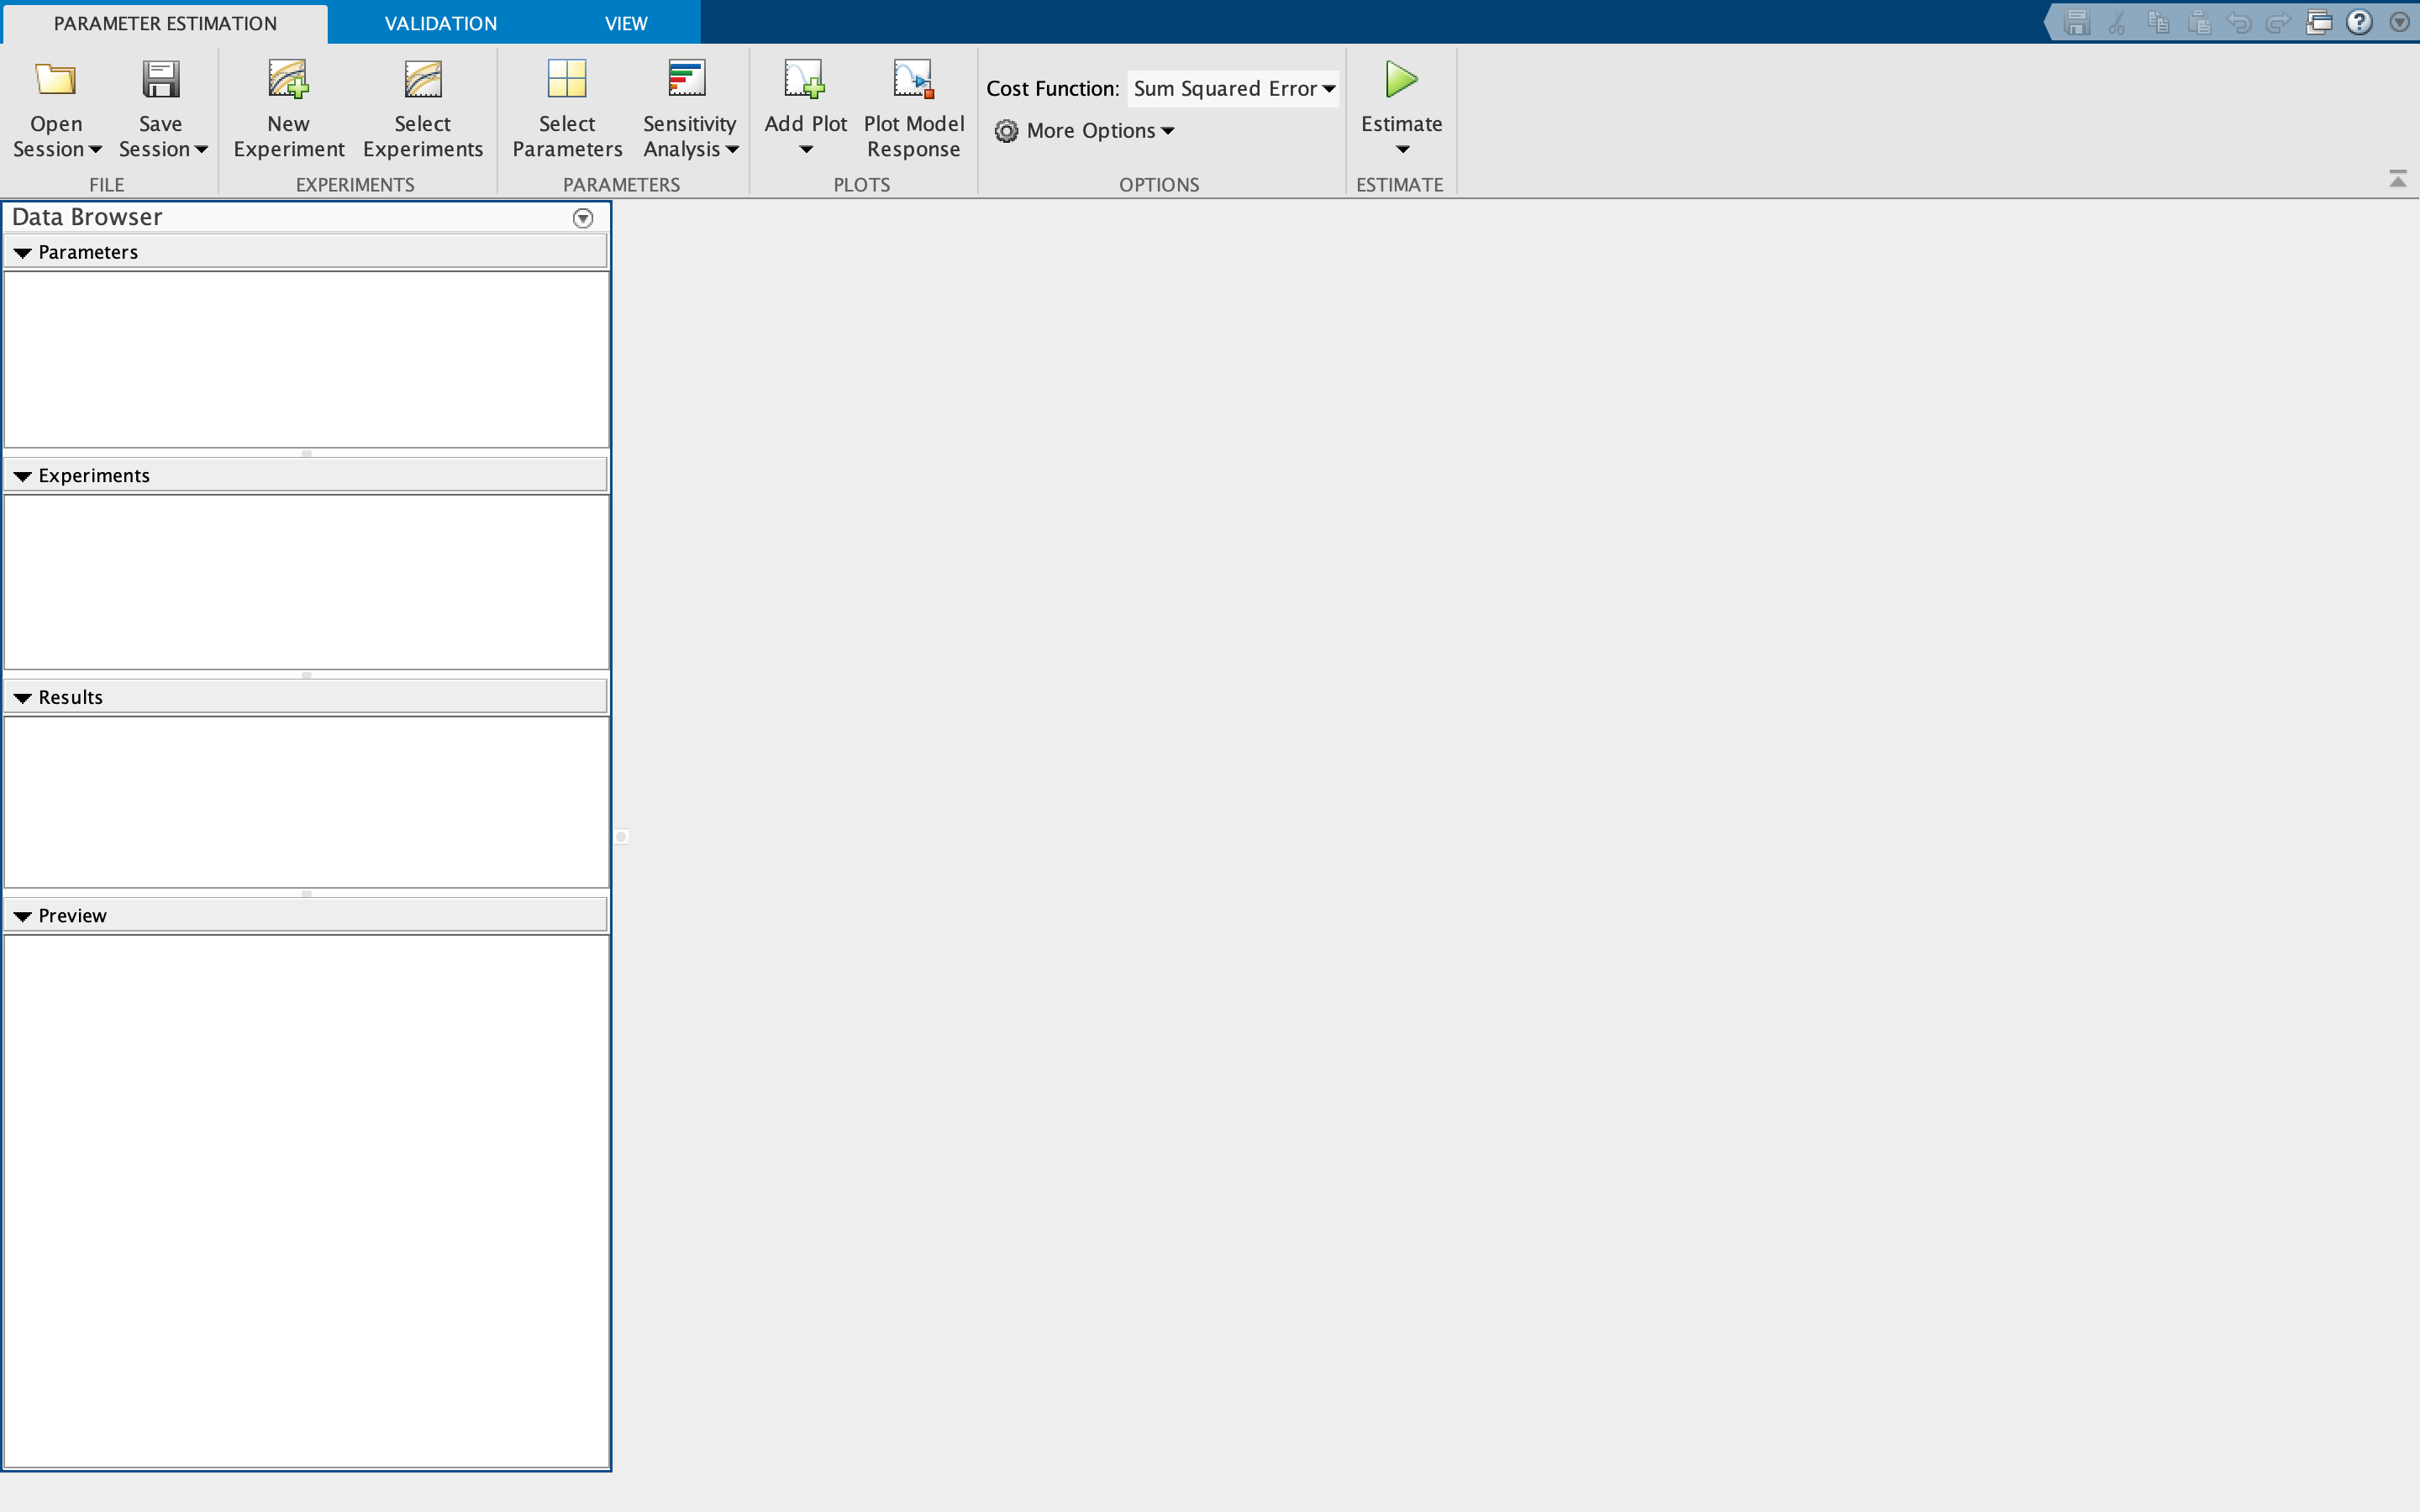
\includegraphics[width=12cm]{../Figures/QuadSimulation/ParameterEstimation/PS_app.png}
%	\centering
%	\caption{جعبه‌ابزار
%	\lr{Parameter Estimator}}
%	\label{PS}
%\end{figure}


%\subsection{تخمین پارامترهای کانال رول موتور خاموش}
برای اصلاح پارامترهای رول چندین آزمایش انجام شد و با استفاده از داده‌های ثبت شده از وضعیت استند در کانال رول و جعبه‌ابزار
\lr{Parameter Estimator}،
پارامترهای کانال رول اصلاح شدند.
برای انجام آزمایش استند از شرایط اولیه مختلف با موتور خاموش رها شد  و از خروجی سنسور داده برداری شد. سپس، مدل و داده‌های ثبت شده‌ی سنسور (وضعیت استند در کانال رول) به جعبه‌ابزار
\lr{Parameter Estimator}
داده‌شد. وضعیت کانال رول استند در شبیه‌سازی و واقعیت بعد از اصلاح پارامترهای کانال رول در شکل‌های
\ref{roll_ml_ps1}, \ref{roll_ml_ps1}, \ref{roll_ml_ps3} و \ref{roll_ml_ps4}
مقایسه شده است.

%\begin{figure}[H]
%	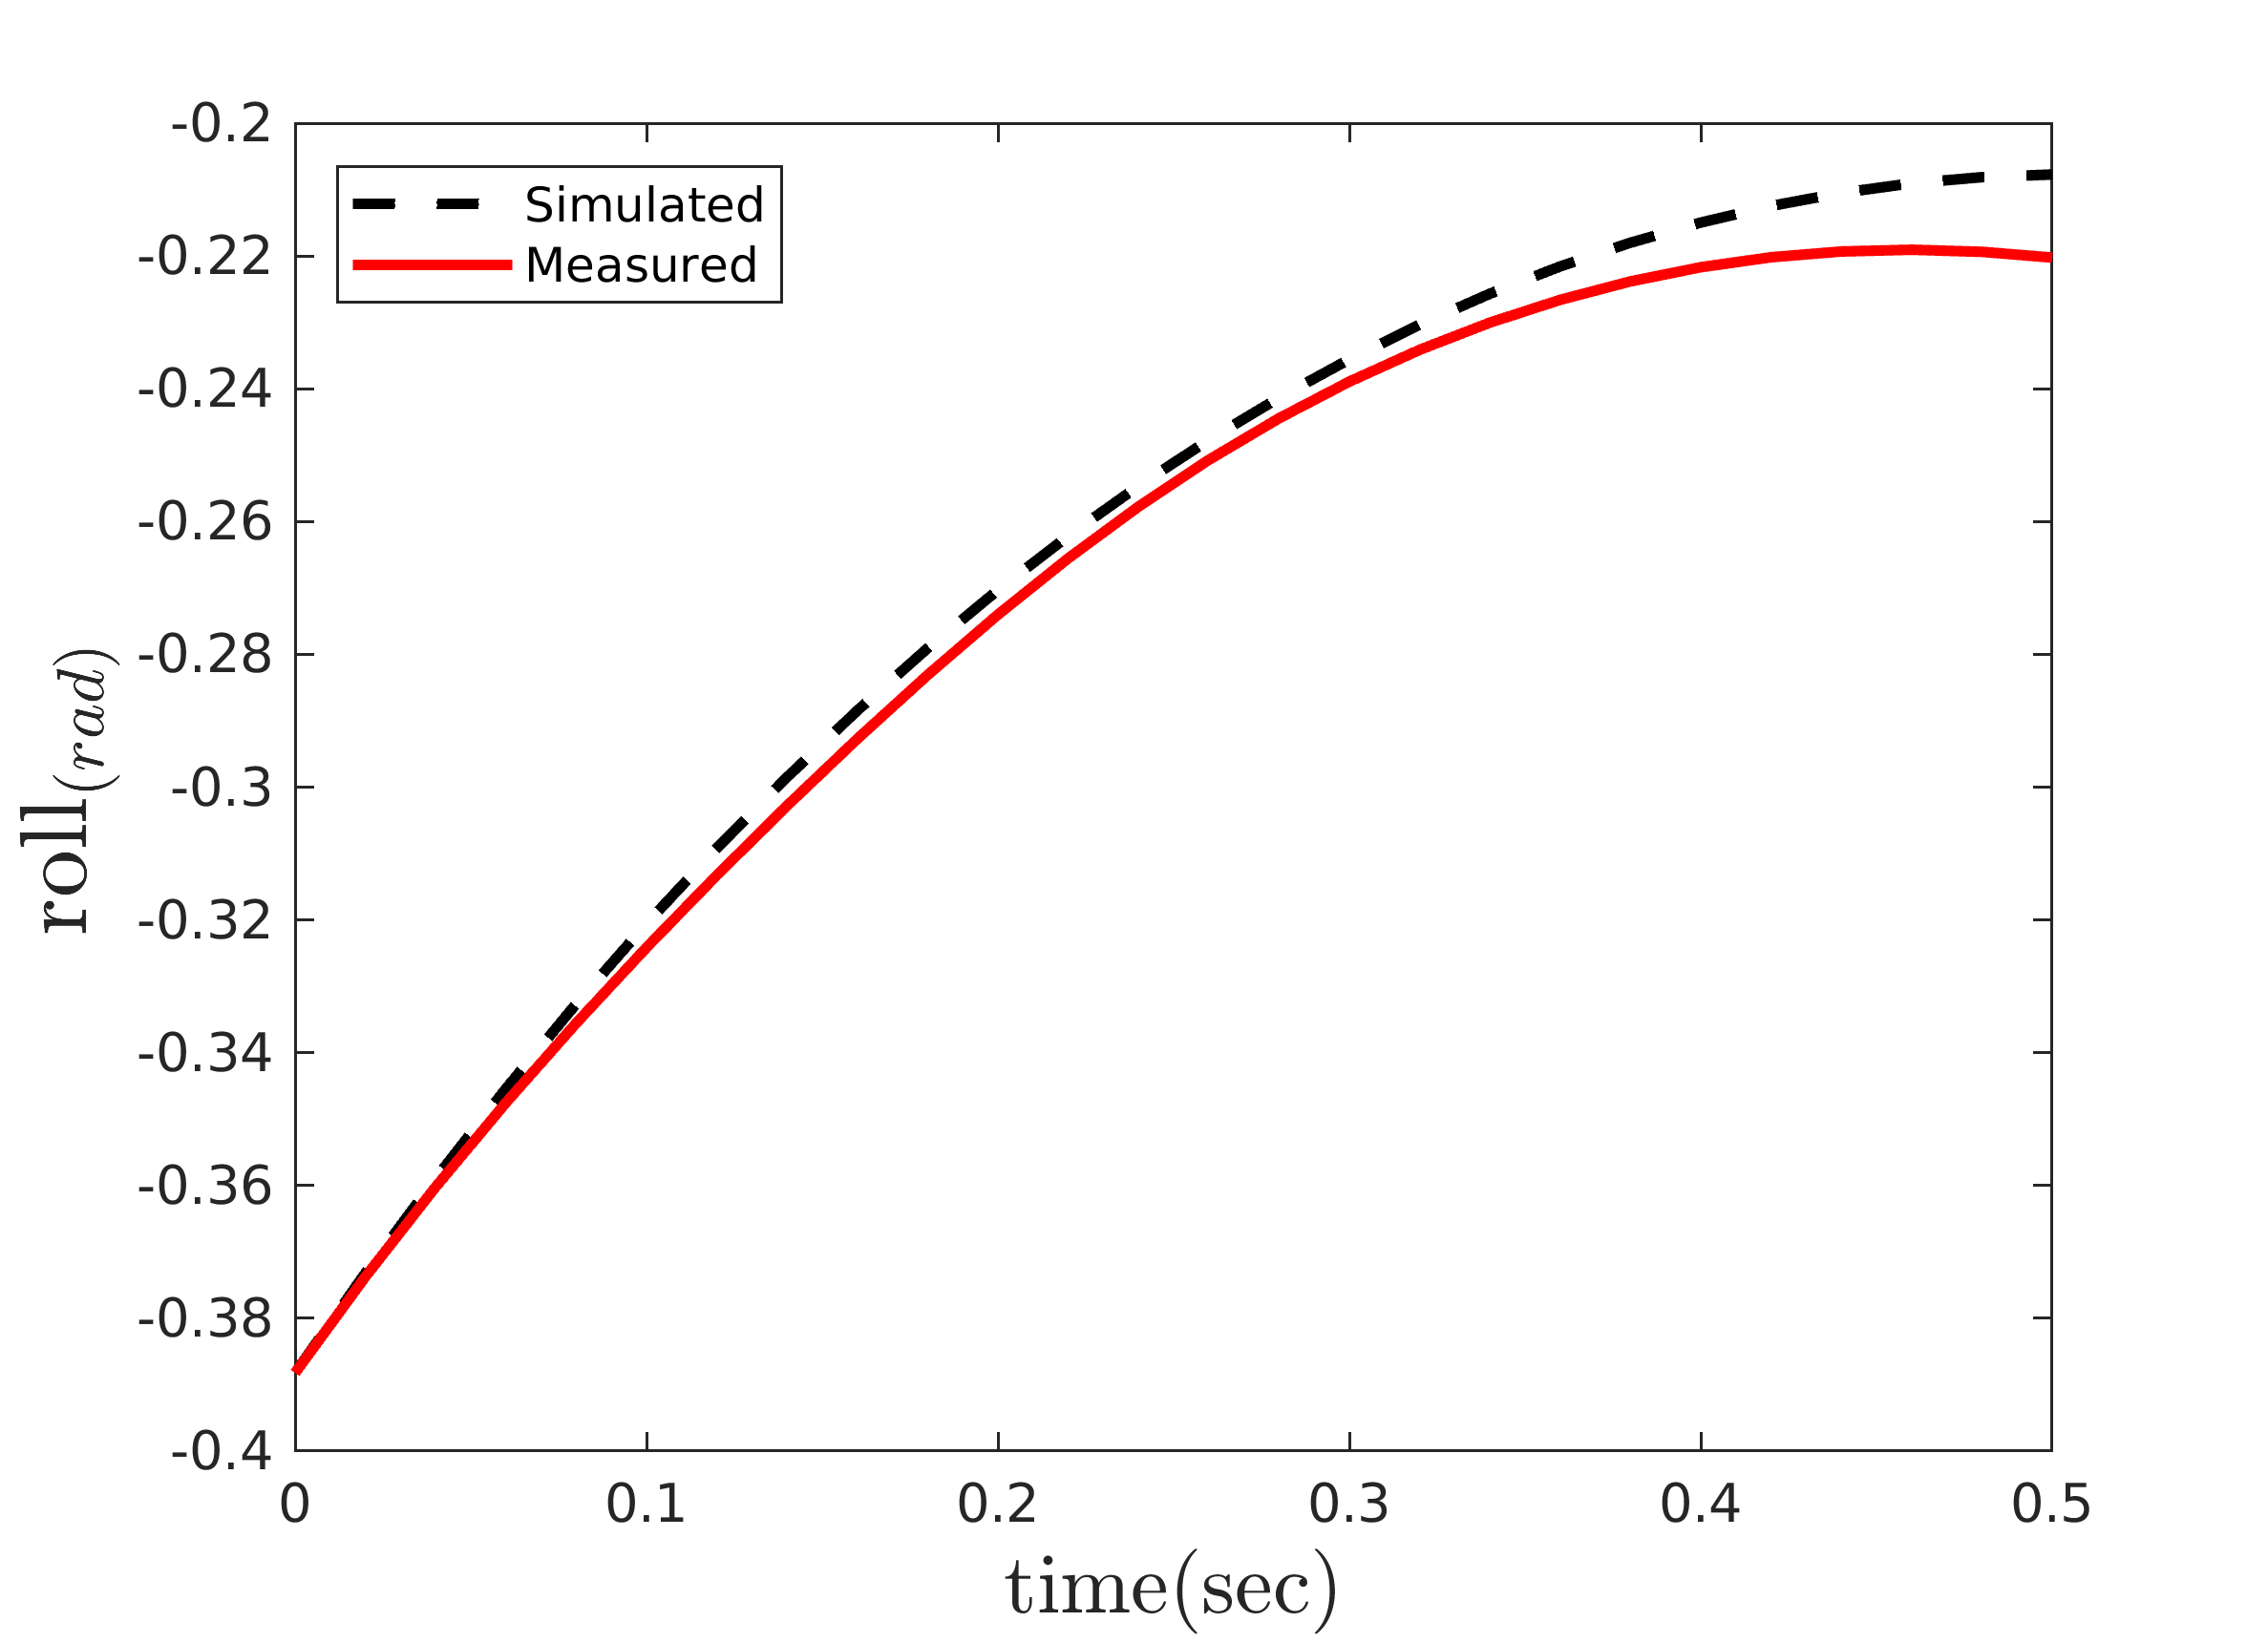
\includegraphics[width=12cm]{../Figures/RCP/roll_ml_parameter_estimation/RCP_roll_S1.png}
%	\centering
%	\caption{مقايسه وضعیت استند در  آزمايش اول و شبیه‌سازی، پس از تخمین پارامترهای کانال رول موتور خاموش}
%	\label{roll_ml_ps1}
%\end{figure}
\begin{figure}[H]
	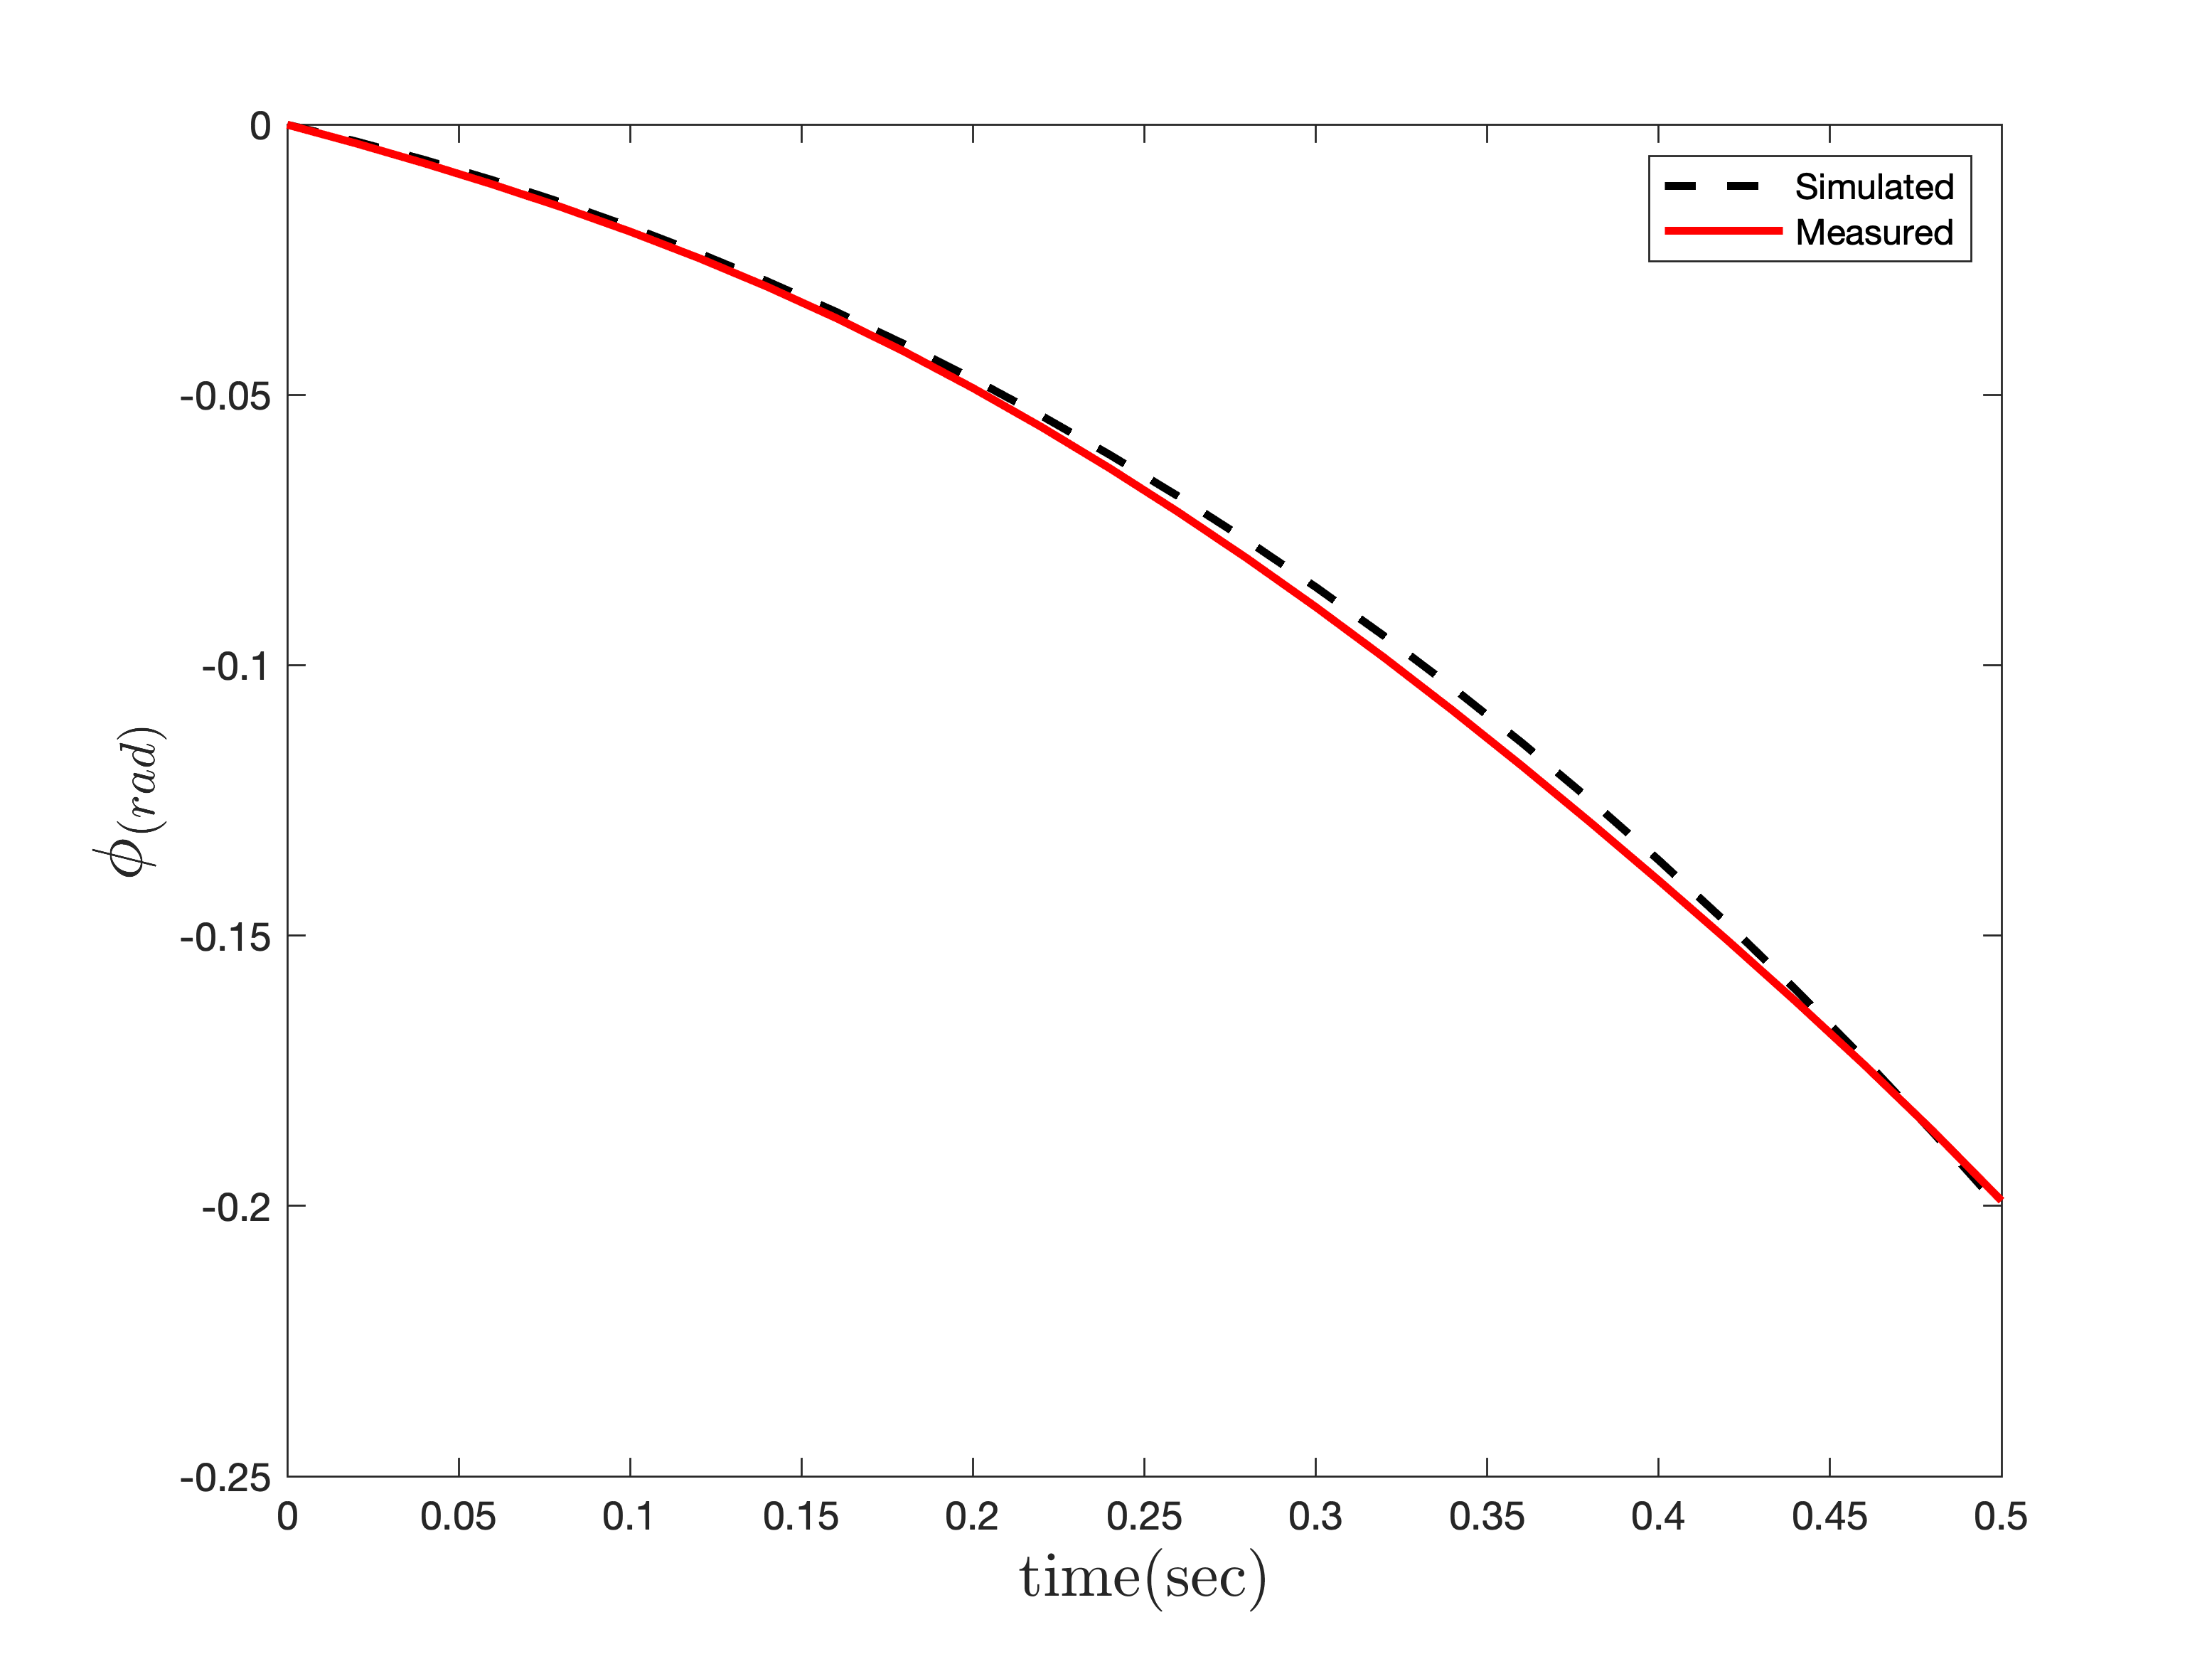
\includegraphics[width=.48\linewidth]{../Figures/RCP/roll_ml_parameter_estimation/RCP_roll_S2.png}
	\centering
	\caption{مقايسه وضعیت استند در  آزمايش دوم و شبیه‌سازی، پس از تخمین پارامترهای کانال رول موتور خاموش}
	\label{roll_ml_ps2}
\end{figure}
%\begin{figure}[H]
%	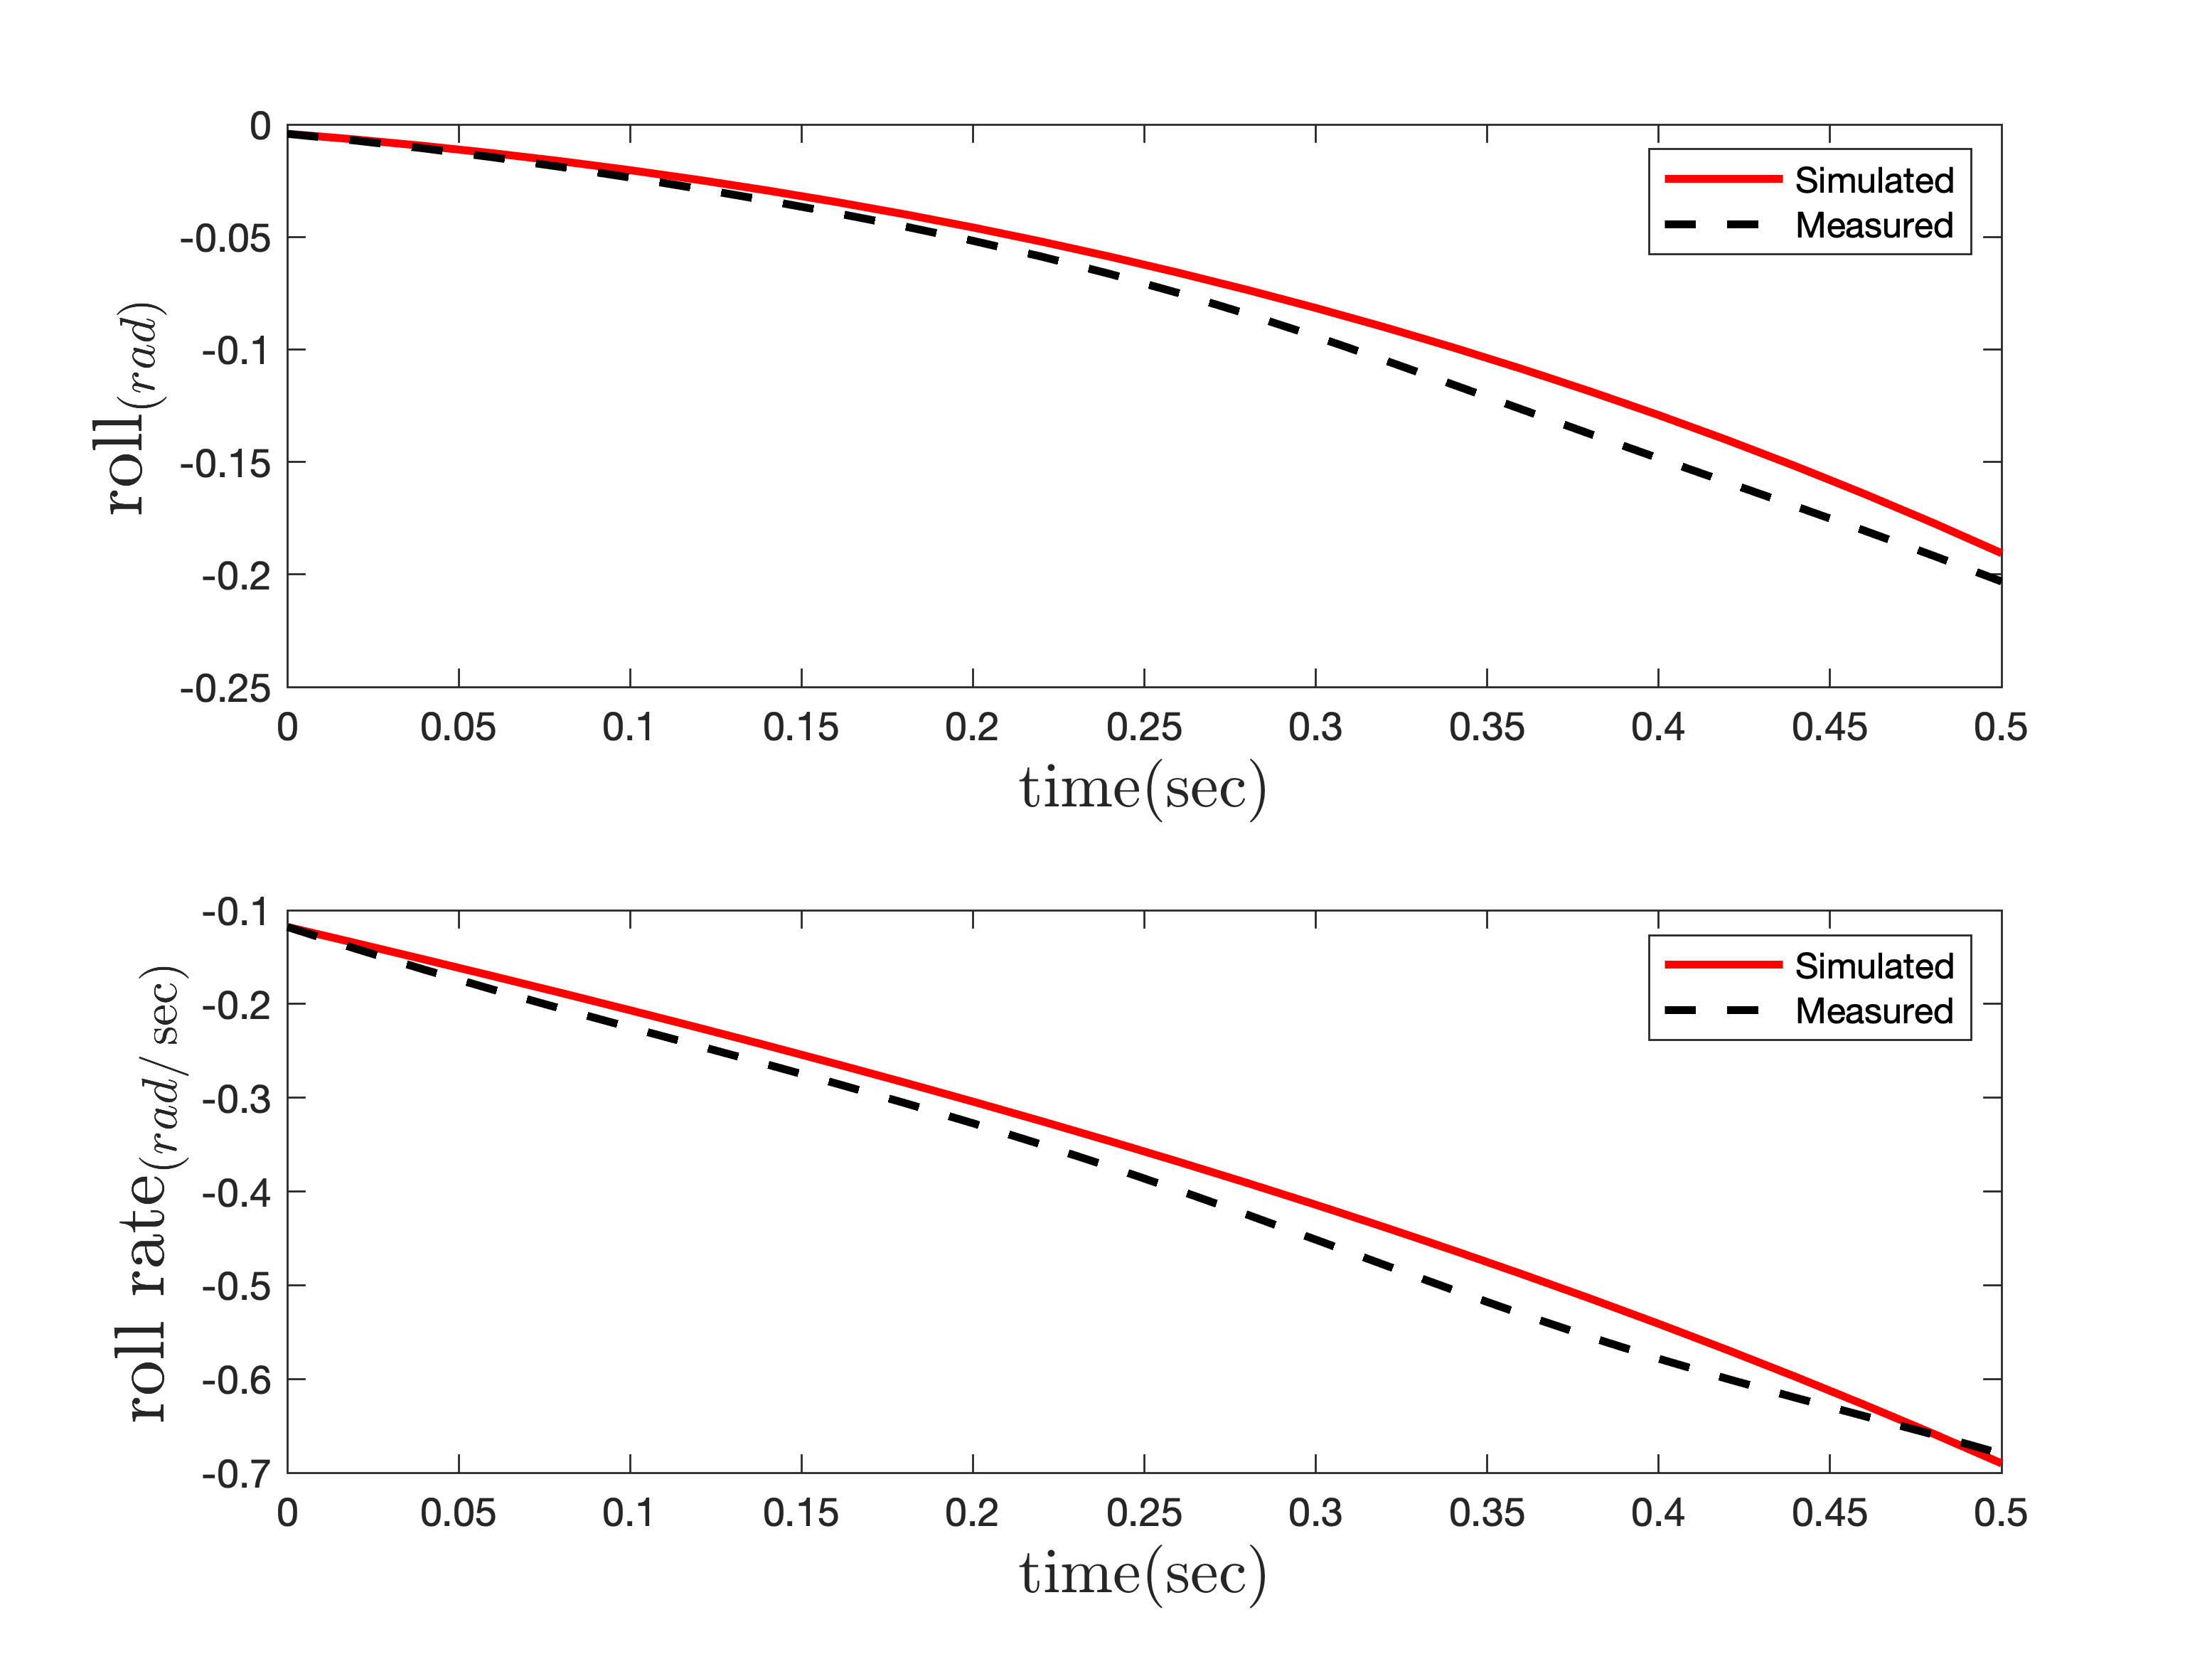
\includegraphics[width=12cm]{../Figures/RCP/roll_ml_parameter_estimation/RCP_roll_S3.png}
%	\centering
%	\caption{مقايسه وضعیت استند در  آزمايش سوم و شبیه‌سازی، پس از تخمین پارامترهای کانال رول موتور خاموش}
%	\label{roll_ml_ps3}
%\end{figure}
%\begin{figure}[H]
%	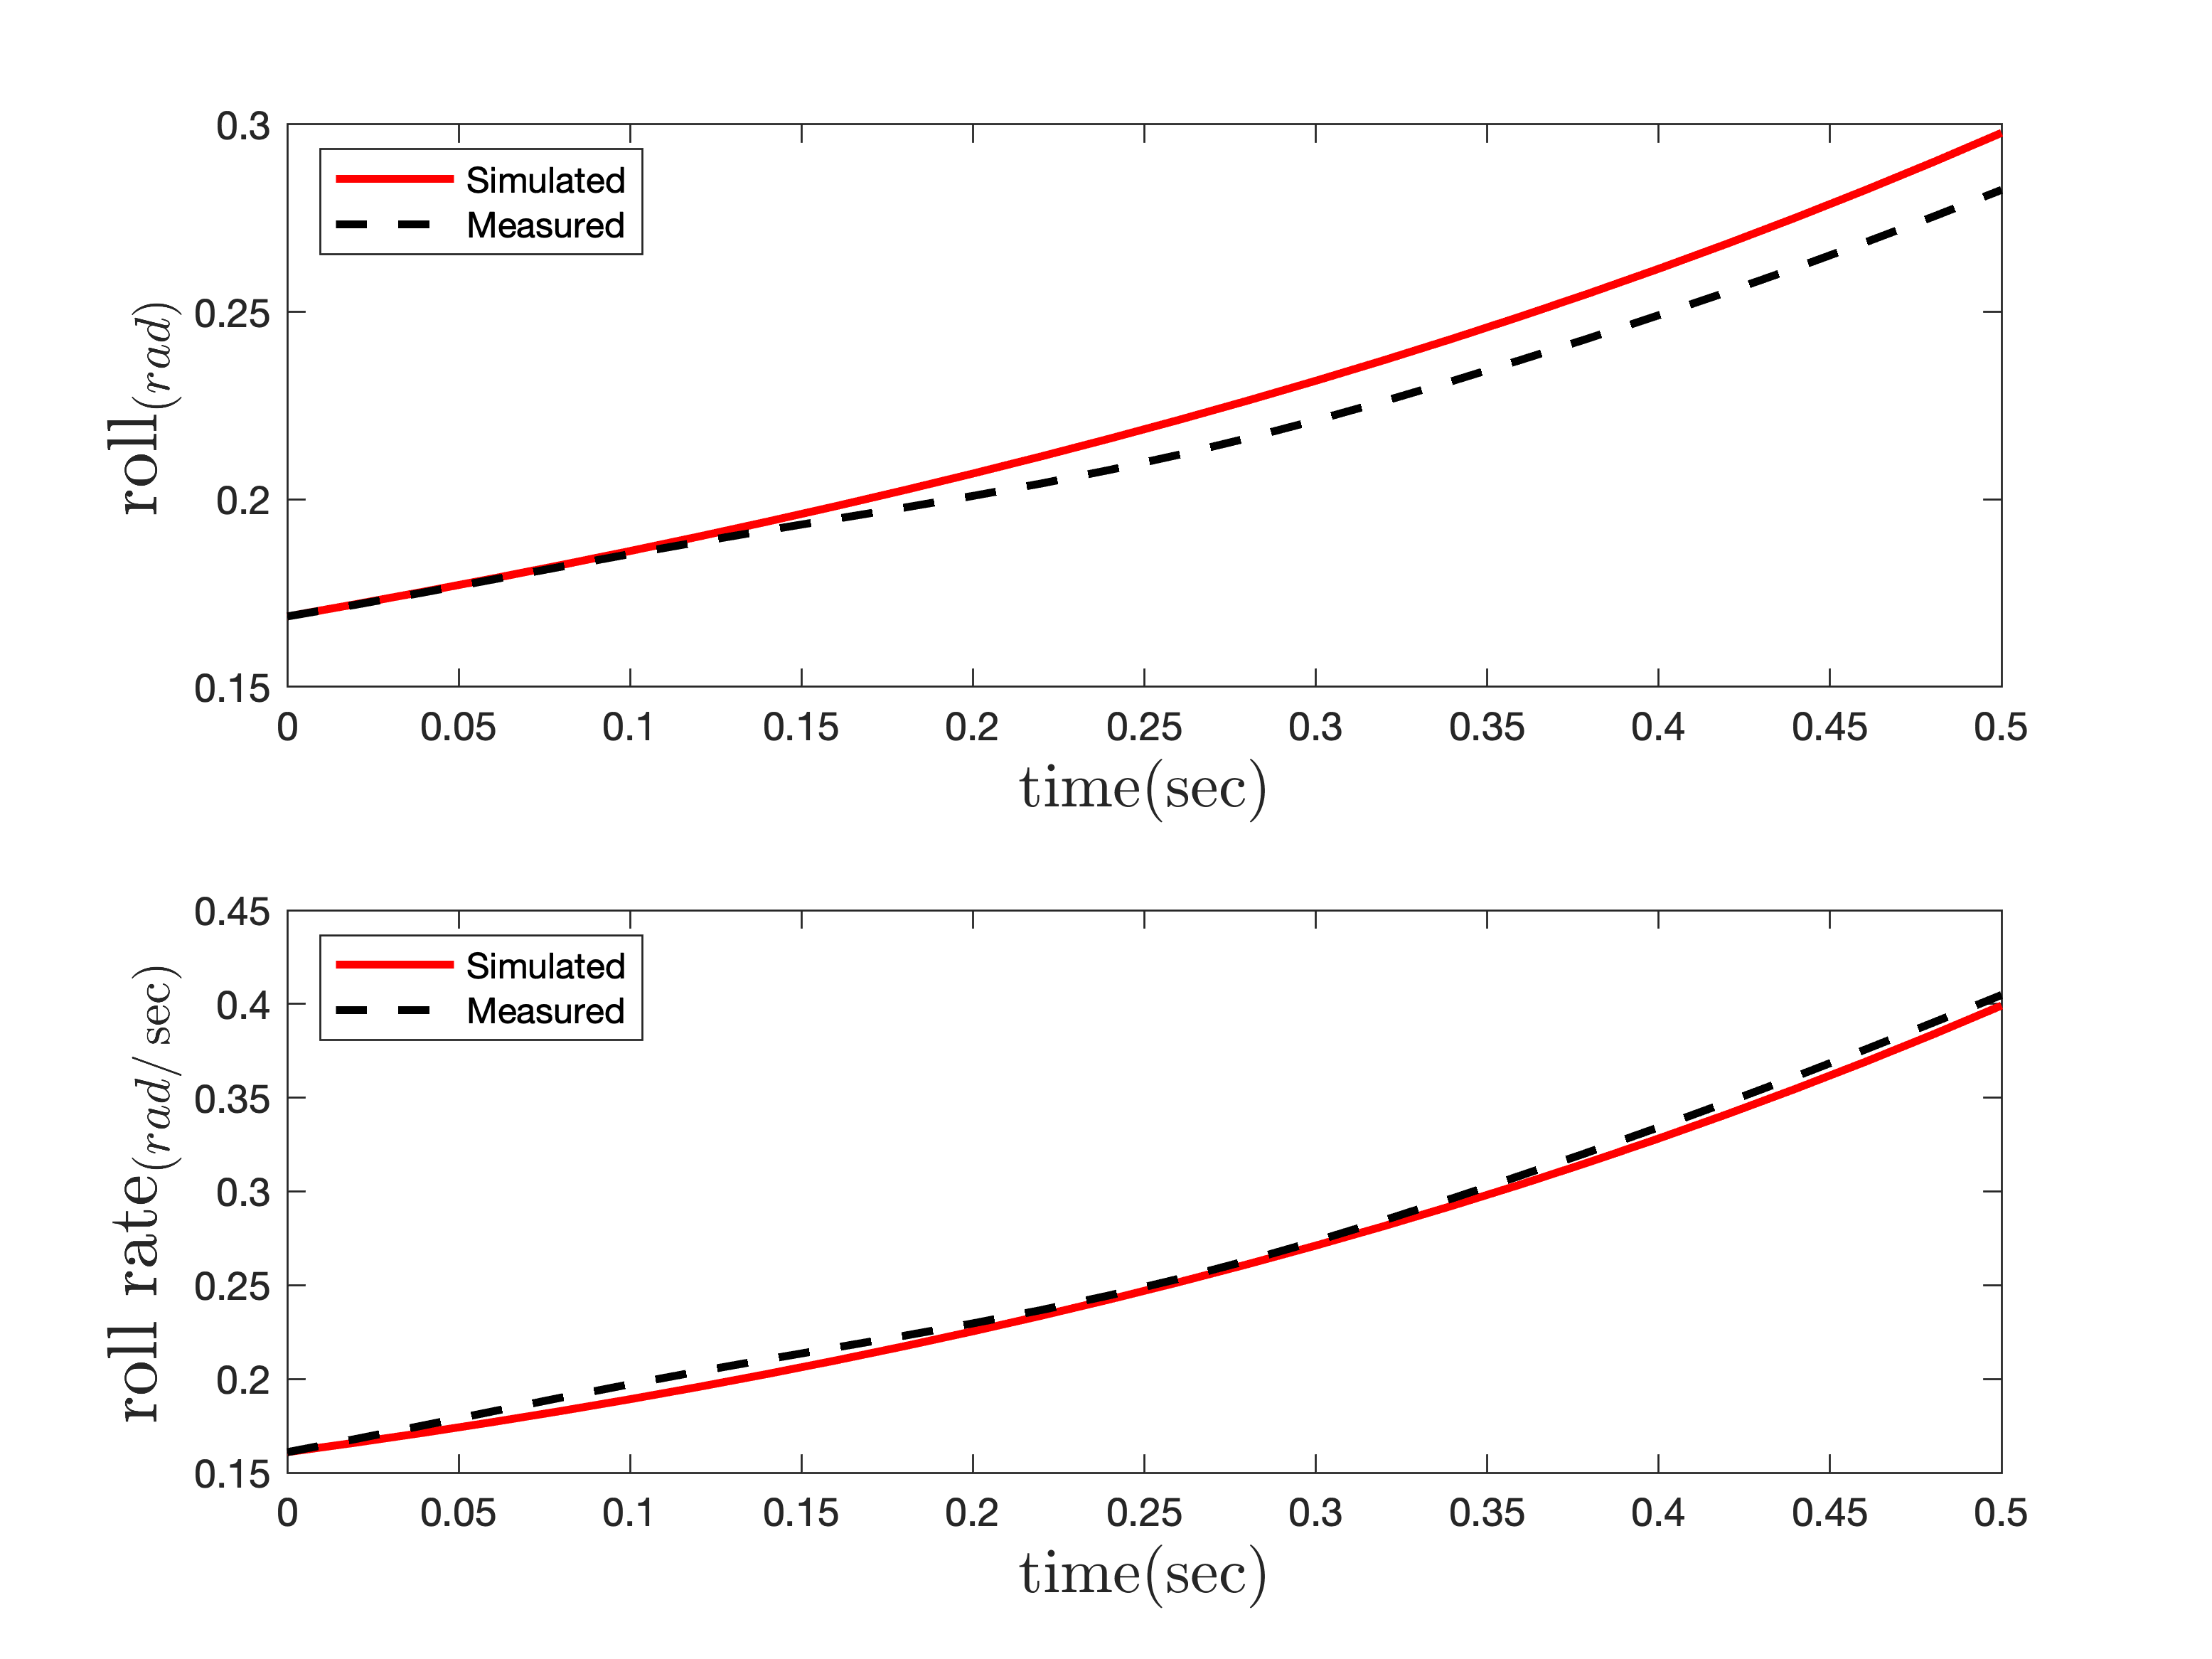
\includegraphics[width=12cm]{../Figures/RCP/roll_ml_parameter_estimation/RCP_roll_S4.png}
%	\centering
%	\caption{مقايسه وضعیت استند در  آزمايش چهارم و شبیه‌سازی، پس از تخمین پارامترهای کانال رول موتور خاموش}
%	\label{roll_ml_ps4}
%\end{figure}

%%\subsection{تخمین پارامترهای کانال رول}
%برای اصلاح پارامترهای رول چندین آزمایش انجام شد و با استفاده از داده‌های ثبت شده از وضعیت استند در کانال رول و جعبه‌ابزار
%\lr{Parameter Estimator}،
%پارامترهای کانال رول اصلاح شدند.
%برای انجام آزمایش هر یک از موتورهای دو و چهار  با دور مختلف شروع به حرکت کردند و از خروجی سنسور داده برداری شد. سپس، مدل و داده‌های ثبت شده‌ی سنسور (وضعیت استند در کانال رول) به جعبه‌ابزار
%\lr{Parameter Estimator}
%داده شد. وضعیت کانال رول استند در شبیه‌سازی و واقعیت بعد از اصلاح پارامترهای کانال رول در شکل‌های
%\ref{roll_ps1}, \ref{roll_ps2}, \ref{roll_ps3}, \ref{roll_ps4} و \ref{roll_ps5}
%مقایسه شده است. 
\hspace*{0.5cm}
در ادامه اصلاح پارامترهای موتور کانال رول چهارپره آورده شده‌است.
\hspace*{0.5cm}





%
%\begin{figure}[H]
%	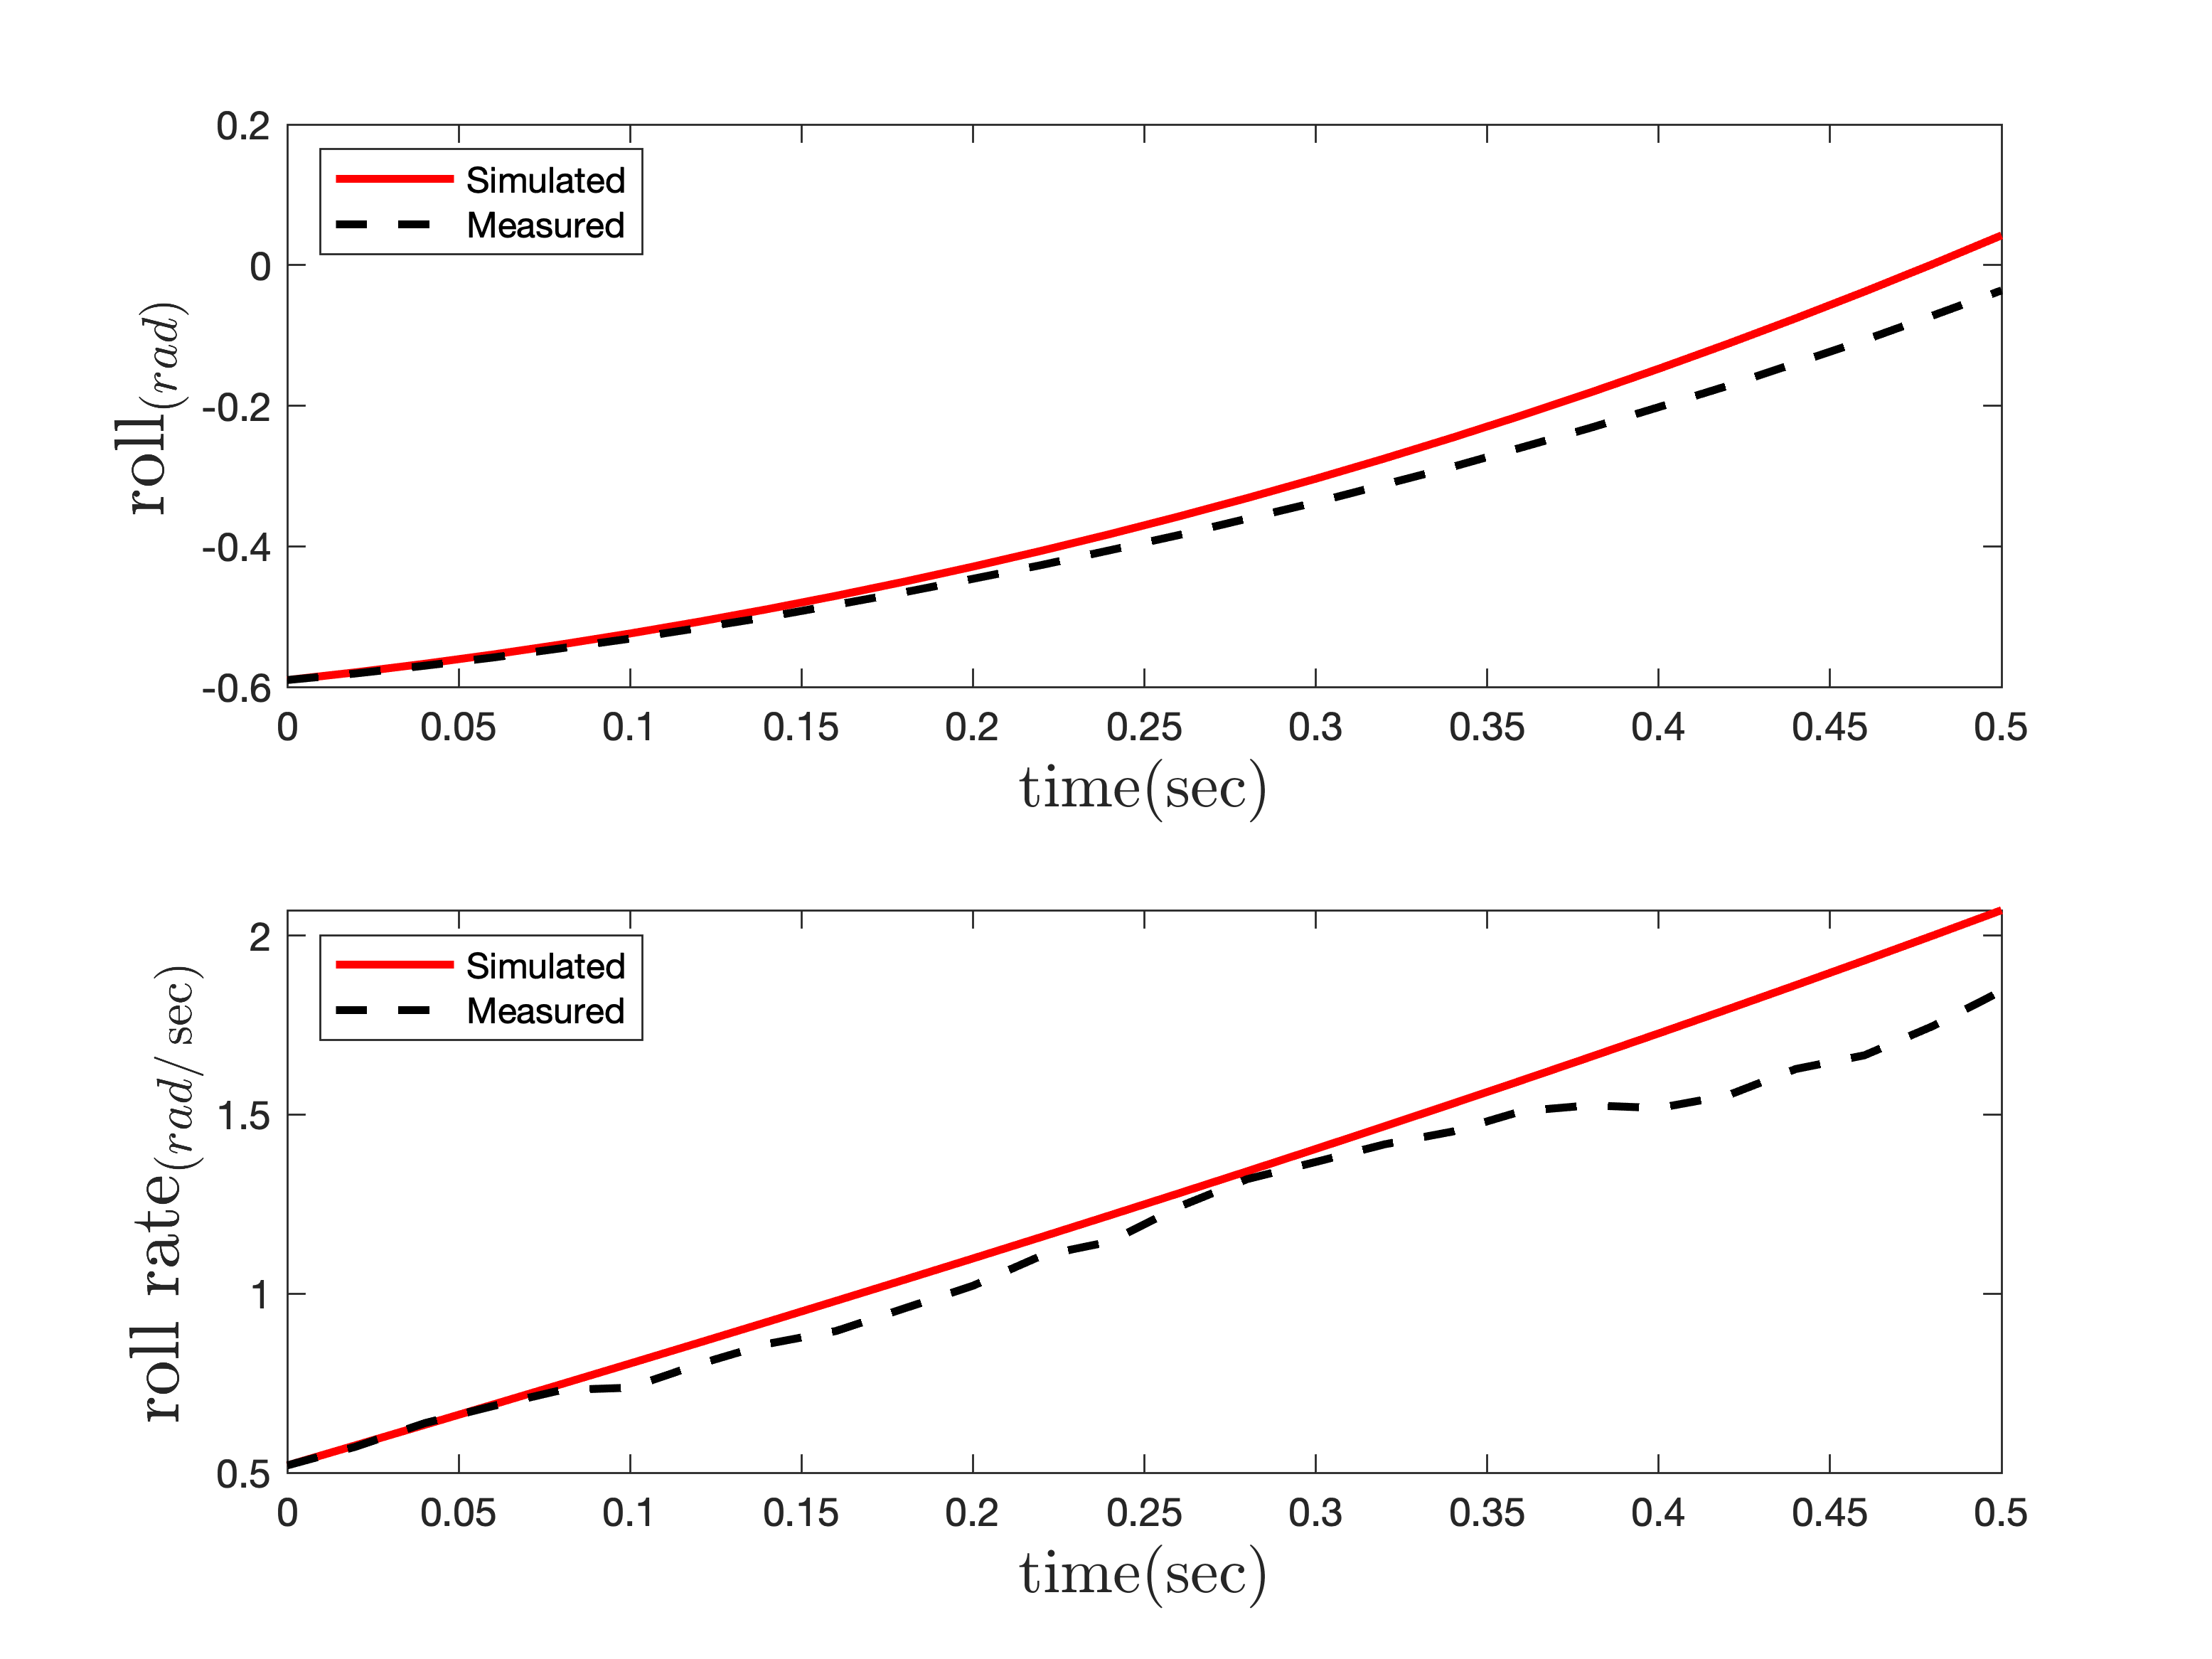
\includegraphics[width=12cm]{../Figures/RCP/roll_parameter_estimation/RCP_roll_S1.png}
%	\centering
%	\caption{مقايسه وضعیت استند در  آزمايش اول و شبیه‌سازی، پس از تخمین پارامترهای کانال رول}
%	\label{roll_ps1}
%\end{figure}
%\begin{figure}[H]
%	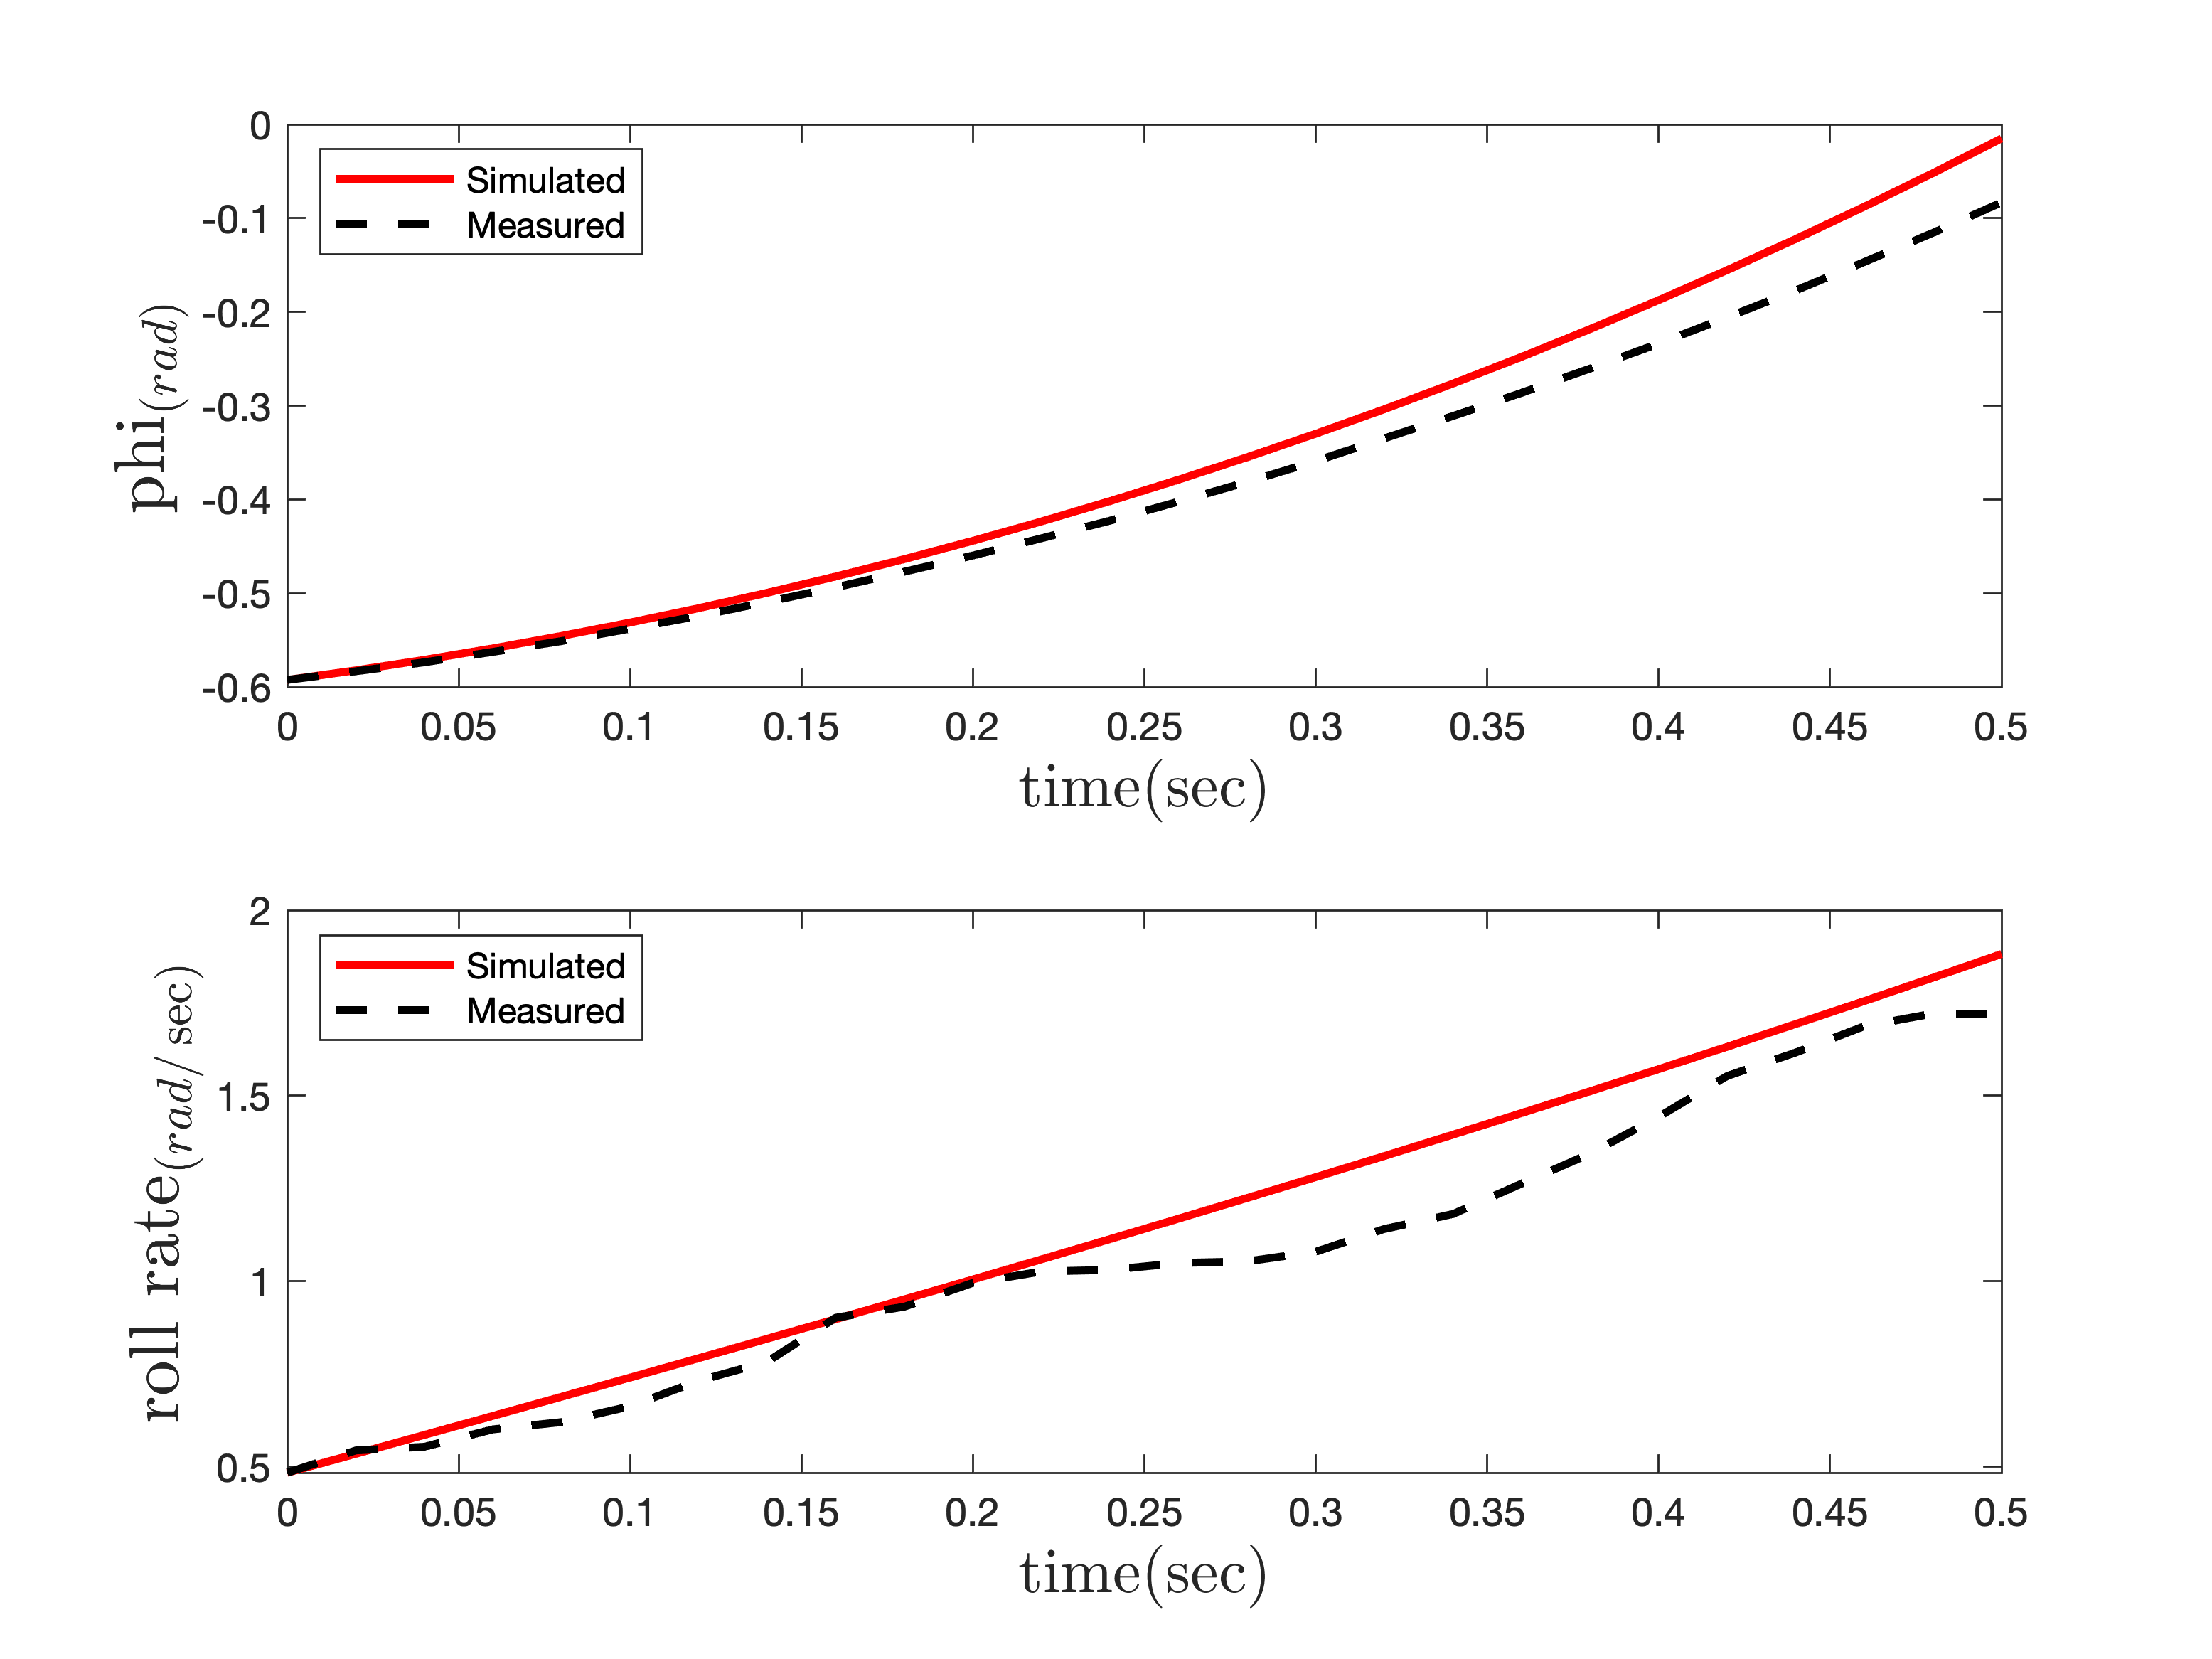
\includegraphics[width=12cm]{../Figures/RCP/roll_parameter_estimation/RCP_roll_S2.png}
%	\centering
%	\caption{مقايسه وضعیت استند در  آزمايش دوم و شبیه‌سازی، پس از تخمین پارامترهای کانال رول}
%	\label{roll_ps2}
%\end{figure}
%\begin{figure}[H]
%	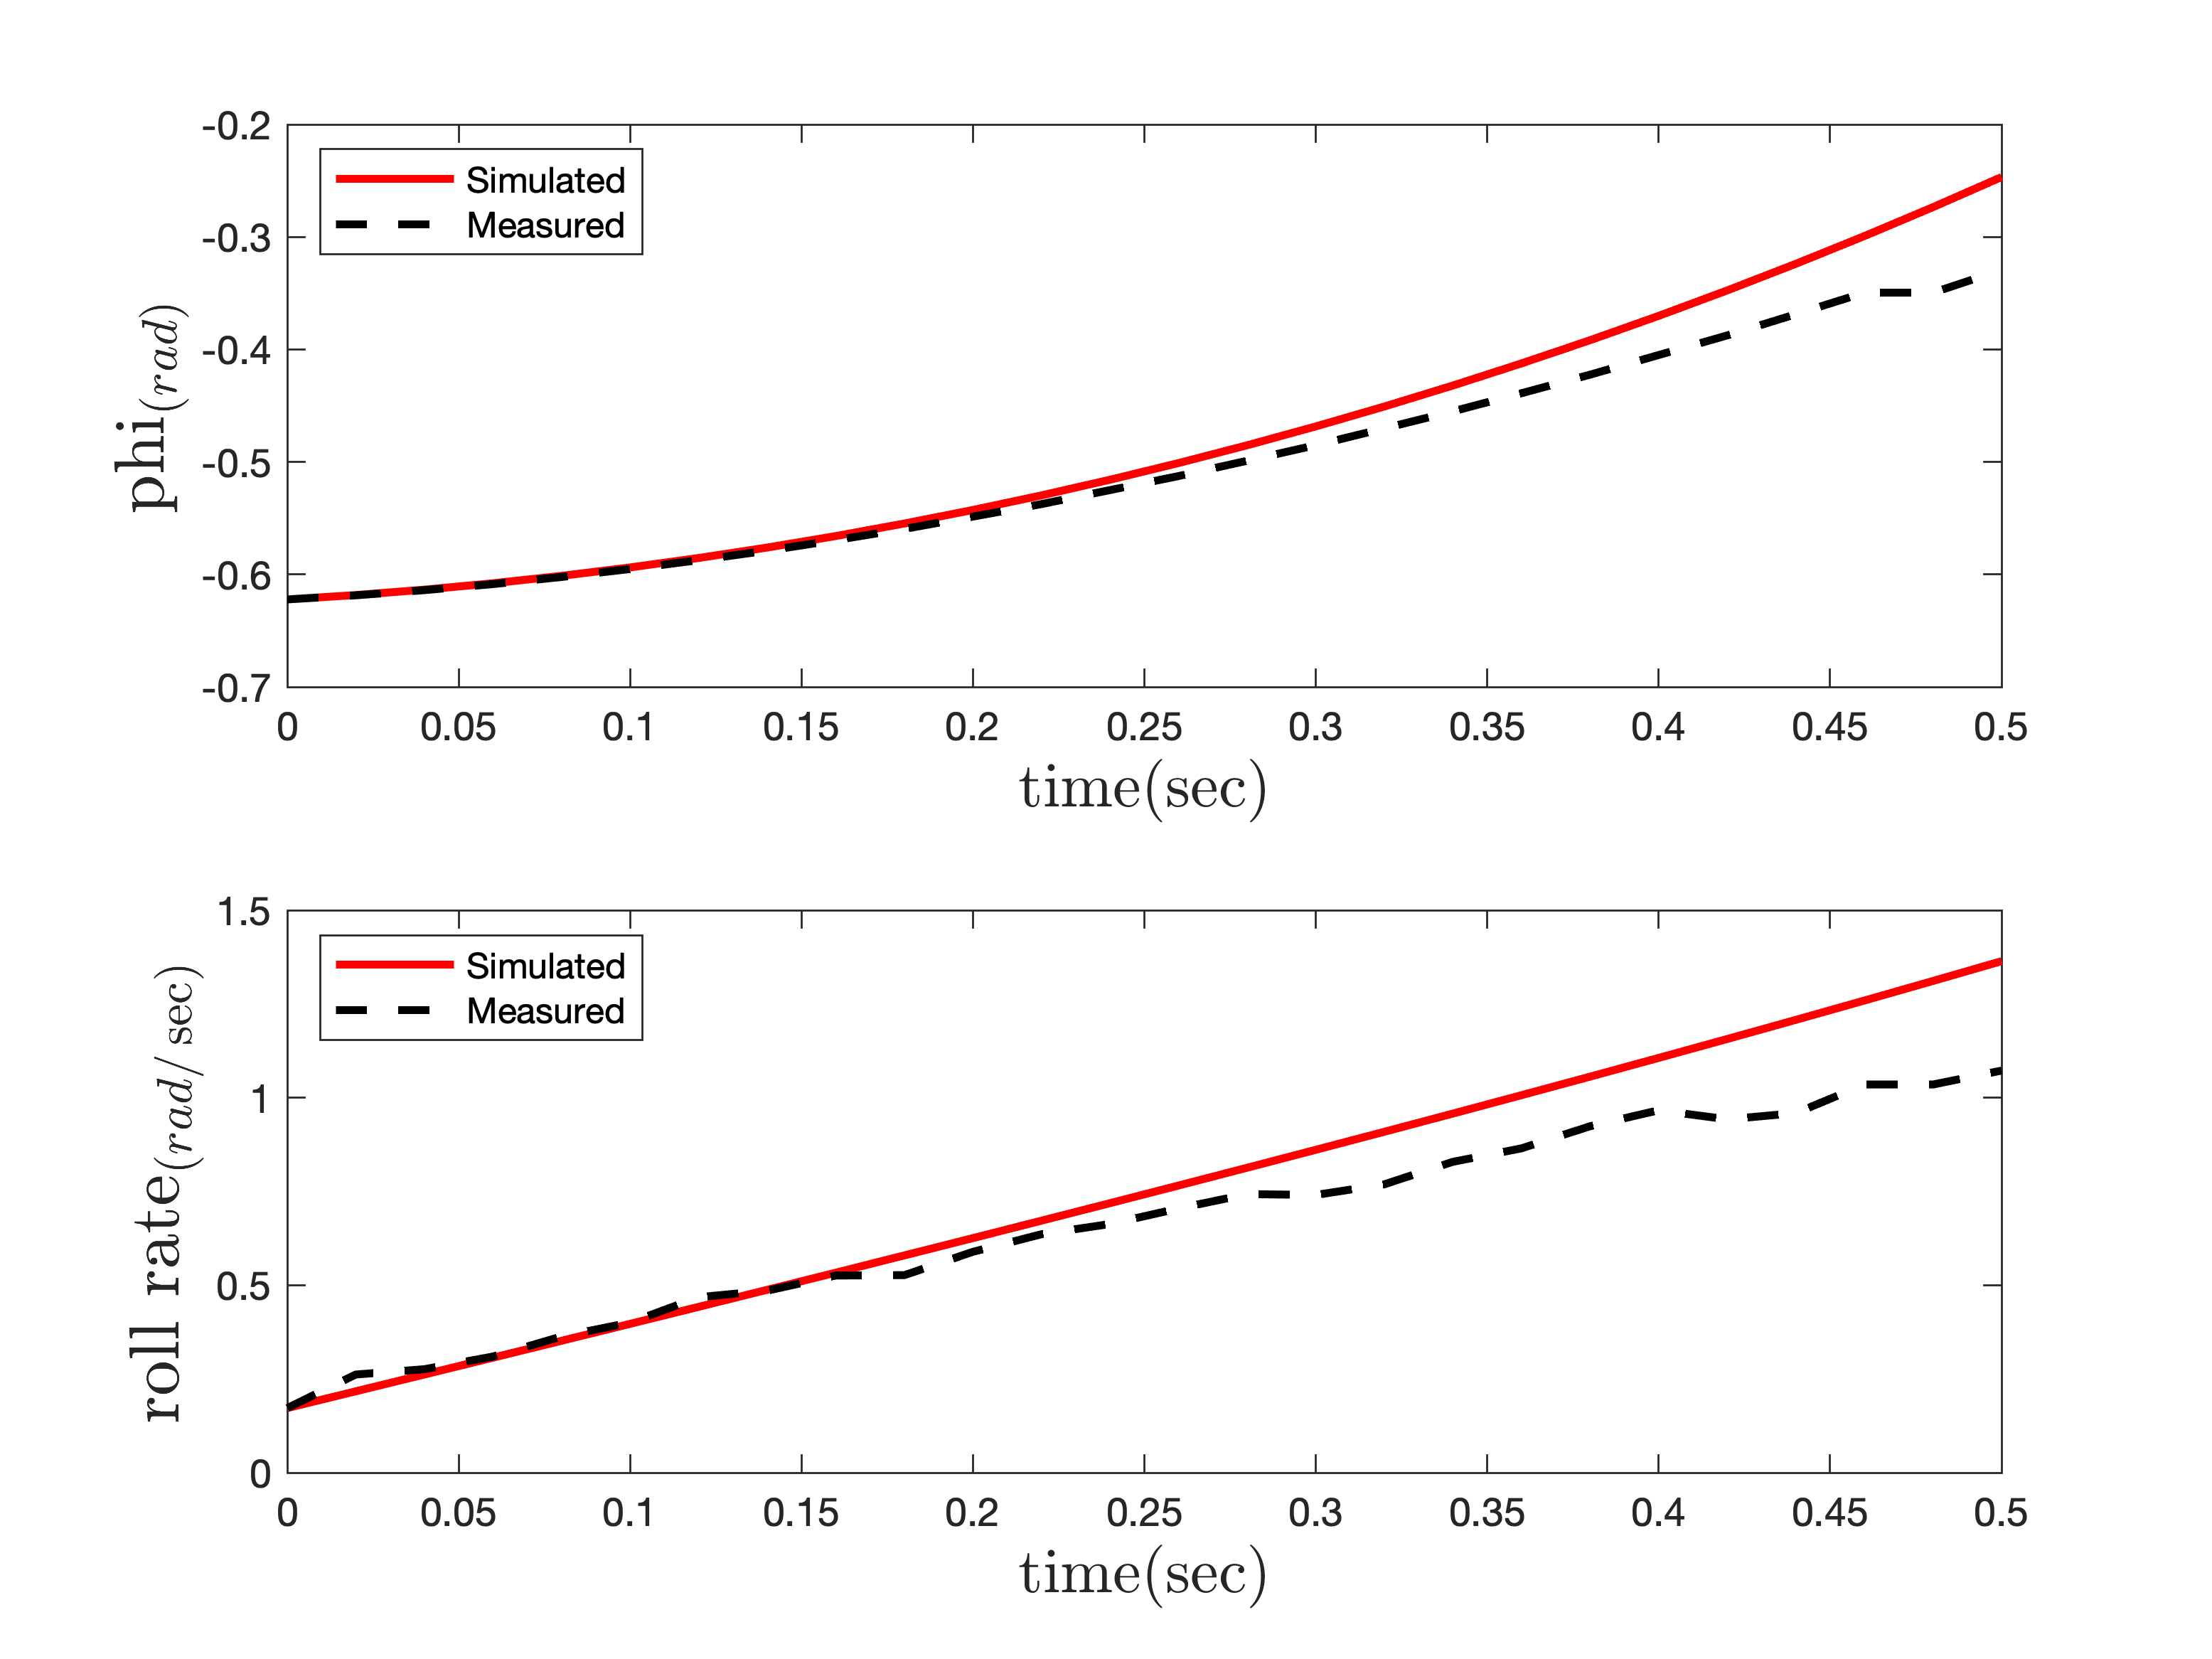
\includegraphics[width=12cm]{../Figures/RCP/roll_parameter_estimation/RCP_roll_S3.png}
%	\centering
%	\caption{مقايسه وضعیت استند در  آزمايش سوم و شبیه‌سازی، پس از تخمین پارامترهای کانال رول}
%	\label{roll_ps3}
%\end{figure}
%\begin{figure}[H]
%	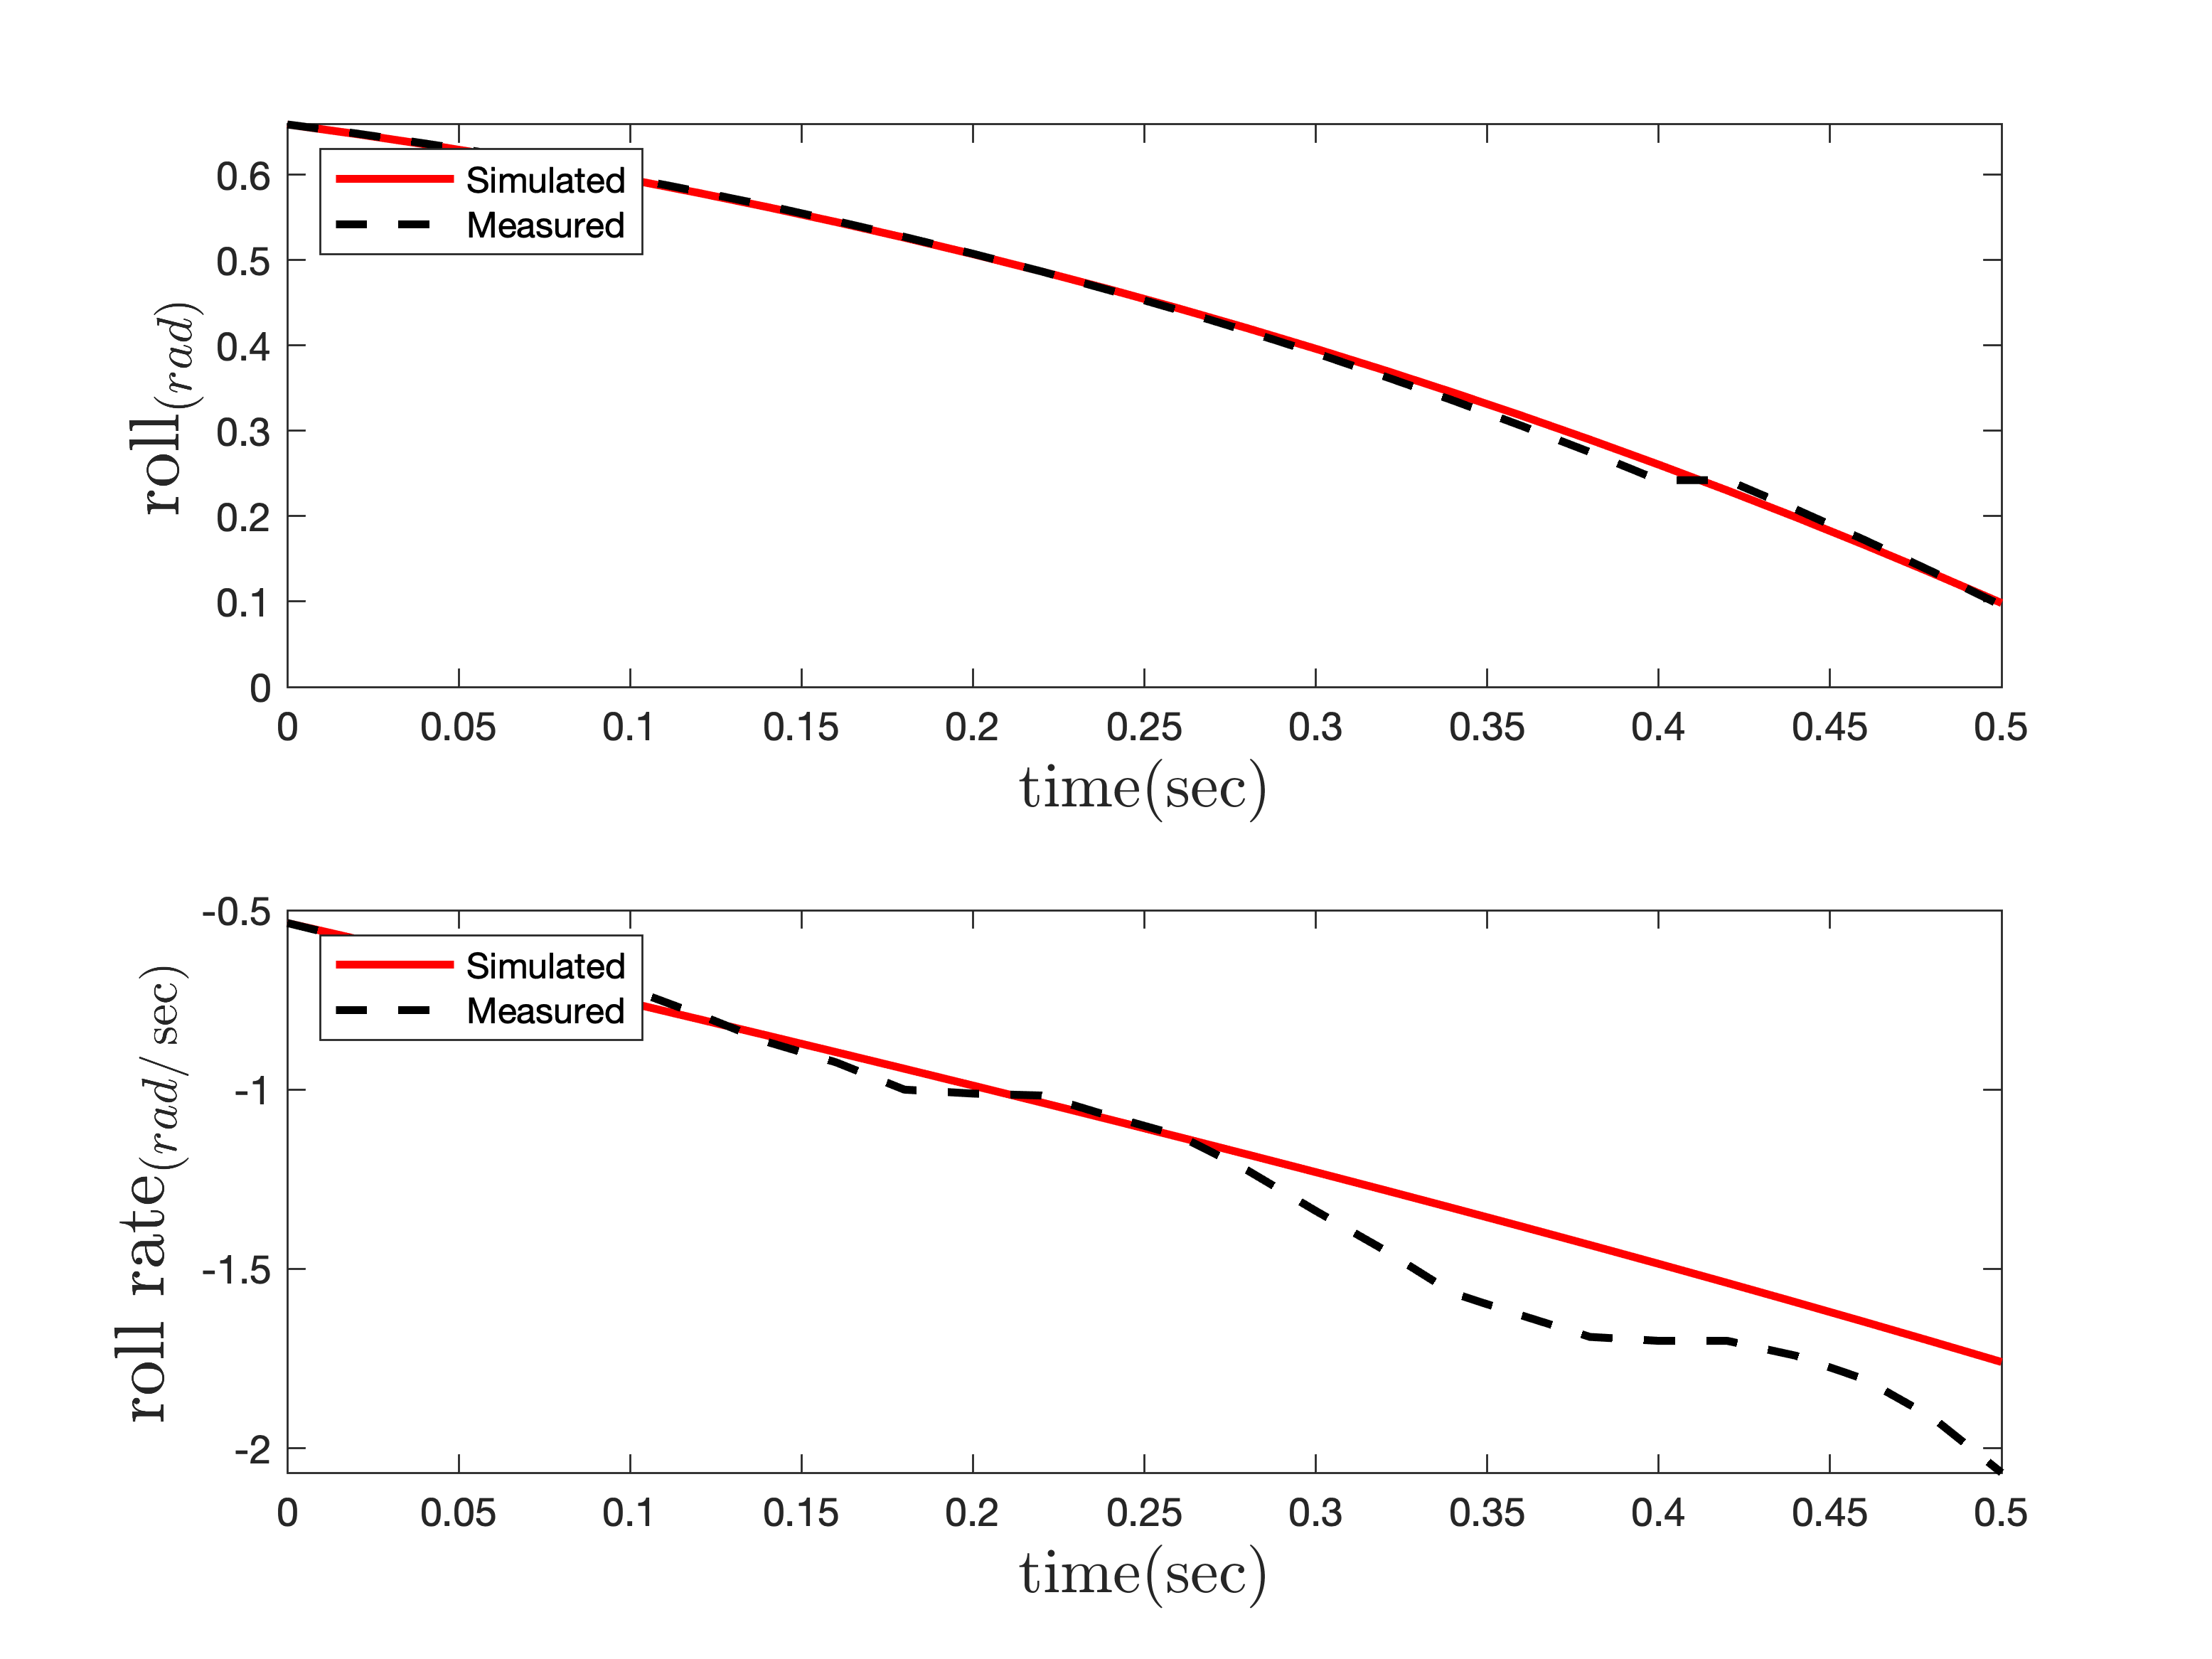
\includegraphics[width=.48\linewidth]{../Figures/RCP/roll_parameter_estimation/RCP_roll_S4.png}
%	\centering
%	\caption{مقايسه وضعیت استند در  آزمايش چهارم و شبیه‌سازی، پس از تخمین پارامترهای کانال رول}
%	\label{roll_ps4}
%\end{figure}
%\begin{figure}[H]
%	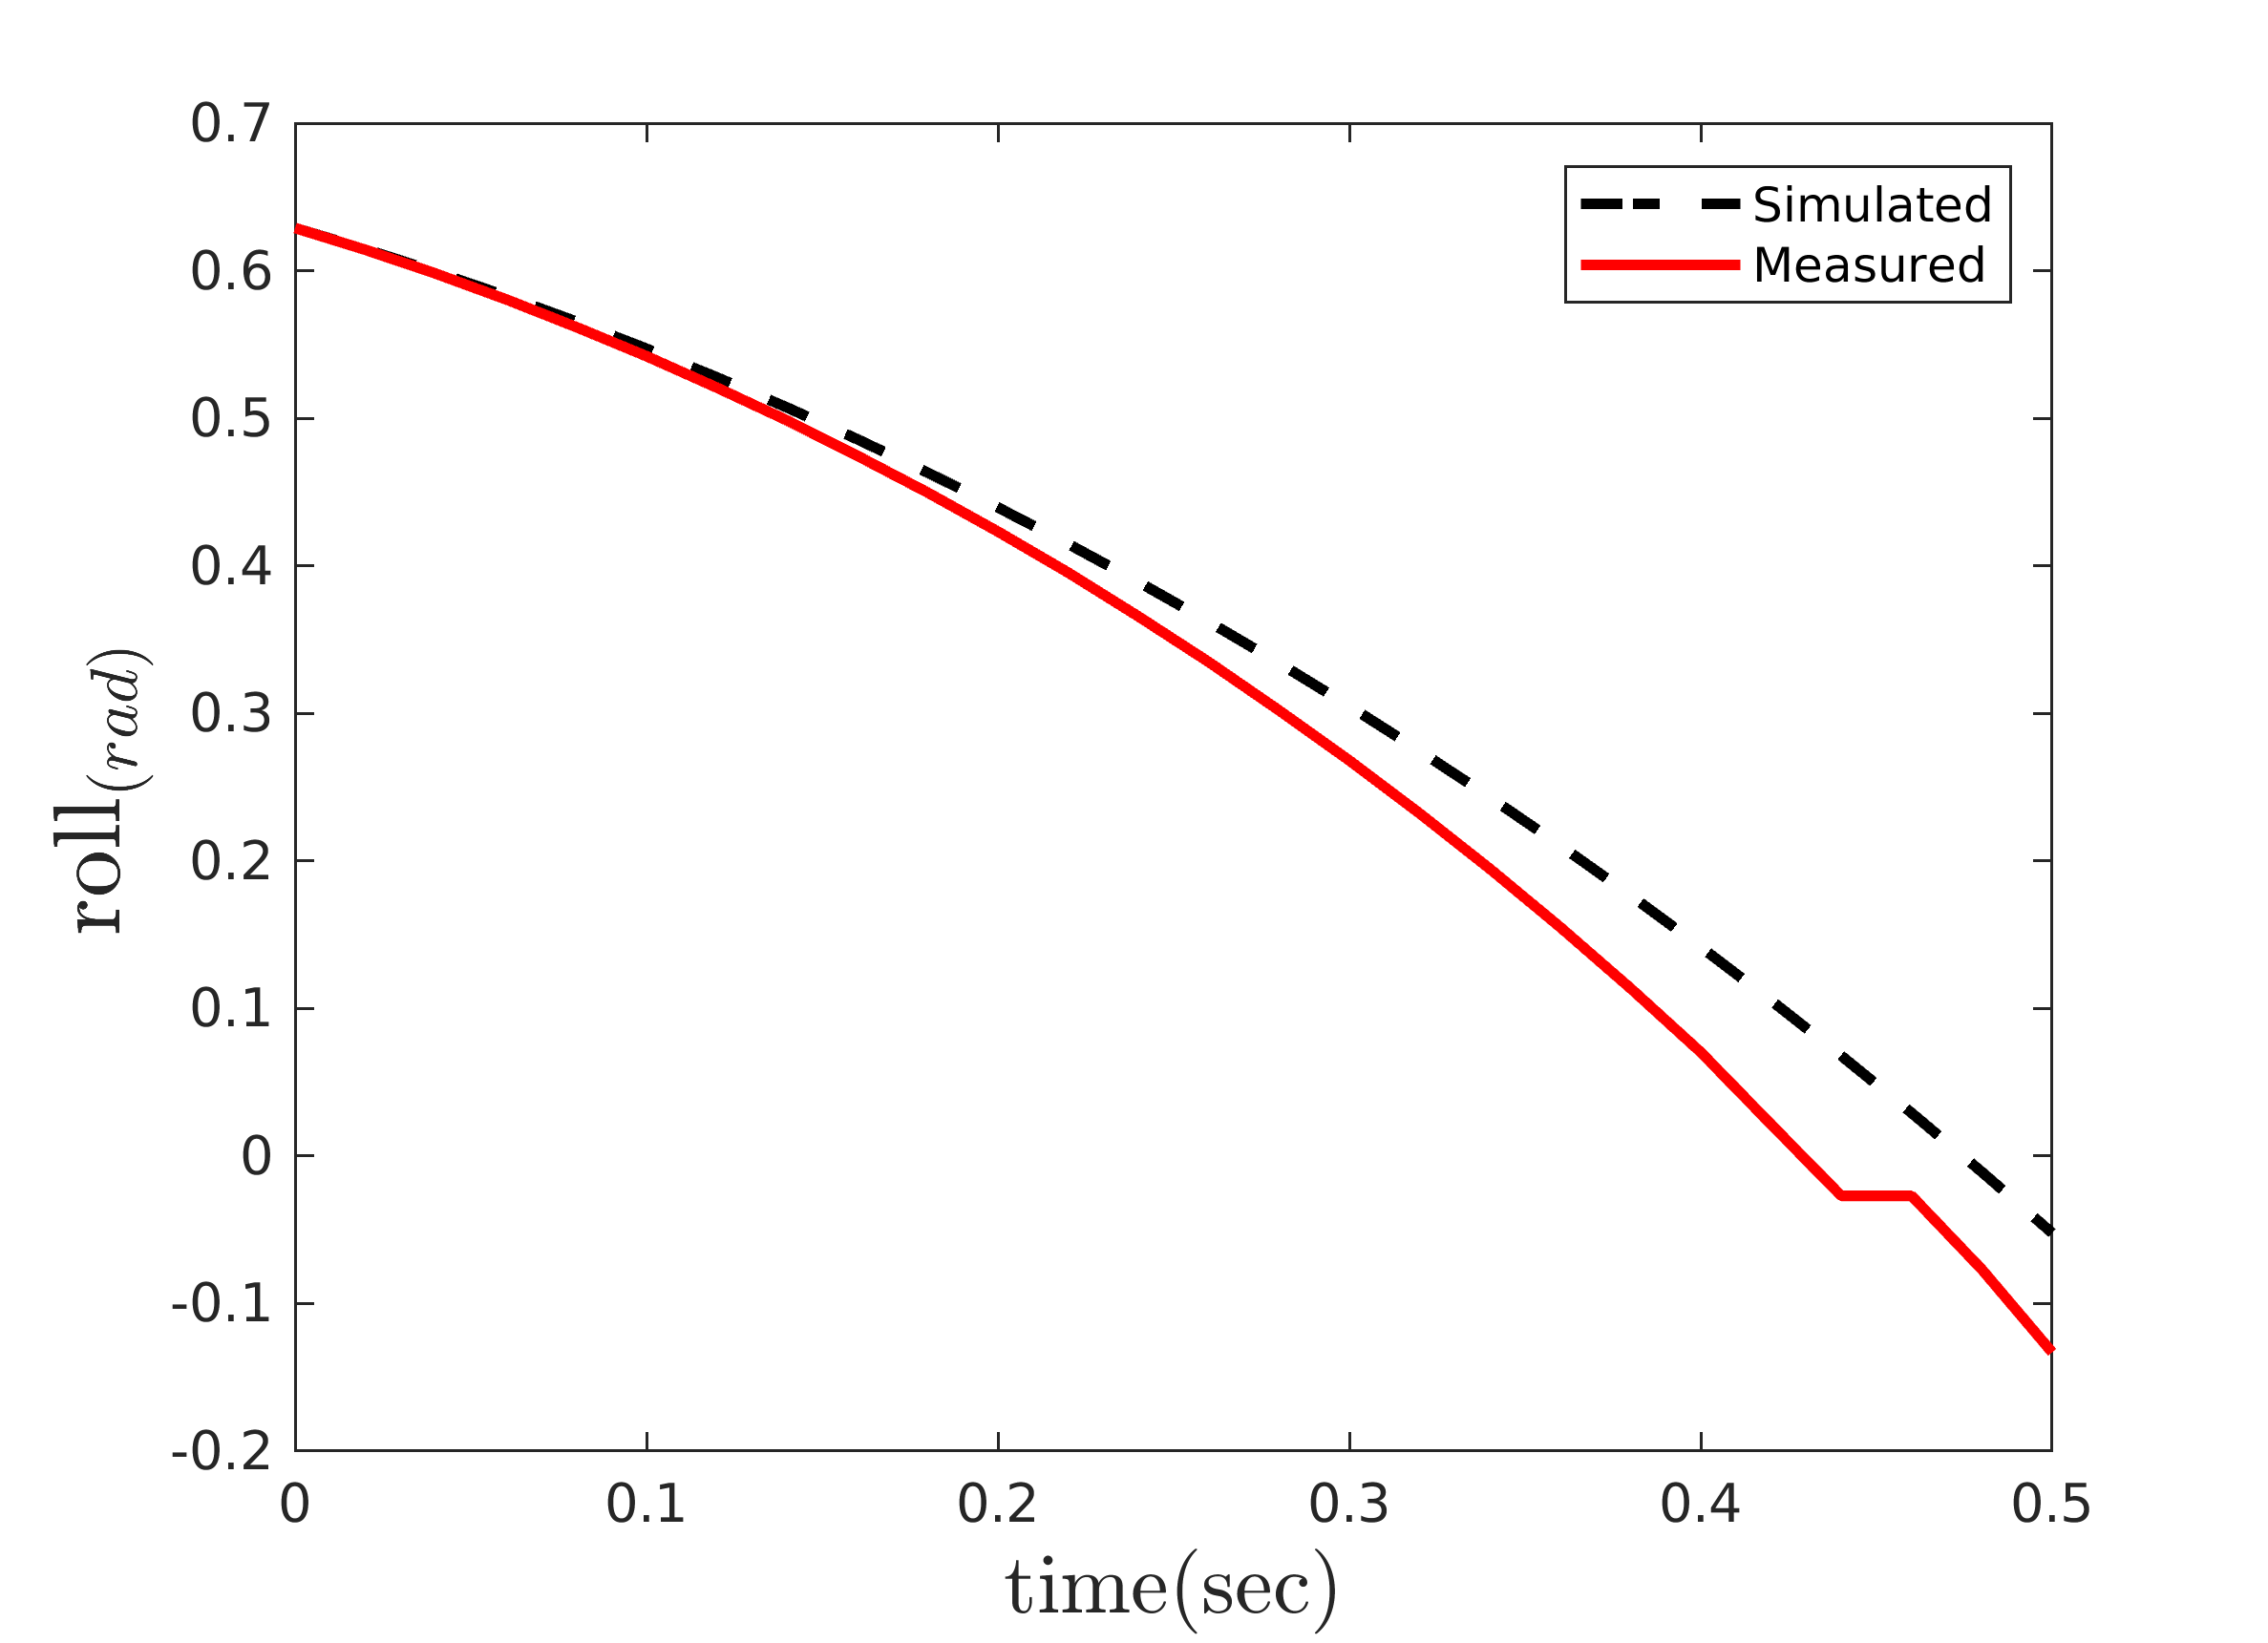
\includegraphics[width=12cm]{../Figures/RCP/roll_parameter_estimation/RCP_roll_S5.png}
%	\centering
%	\caption{مقايسه وضعیت استند در  آزمايش پنجم و شبیه‌سازی، پس از تخمین پارامترهای کانال رول}
%	\label{roll_ps5}
%\end{figure}
  \begin{minipage}[H]{\linewidth}
	\hfill
	\begin{minipage}[b]{0.49\linewidth}
		\centering
		\begin{tabular}{ccc}\hline
			پارامتر & مقدار پارامتر  & مقدار پارامتر بعد از اصلاح
			\\ \hline
			$A_3$  & $1.1\times10^{-4}$ & $5.47\times10^{-5}$ \\\\
			\\\\\\
		\end{tabular}
		\captionof{table}{مقايسه پارامترهای کانال رول قبل و بعد از اصلاح}
	\end{minipage}
	\begin{minipage}[b]{0.48\linewidth}
		\centering
		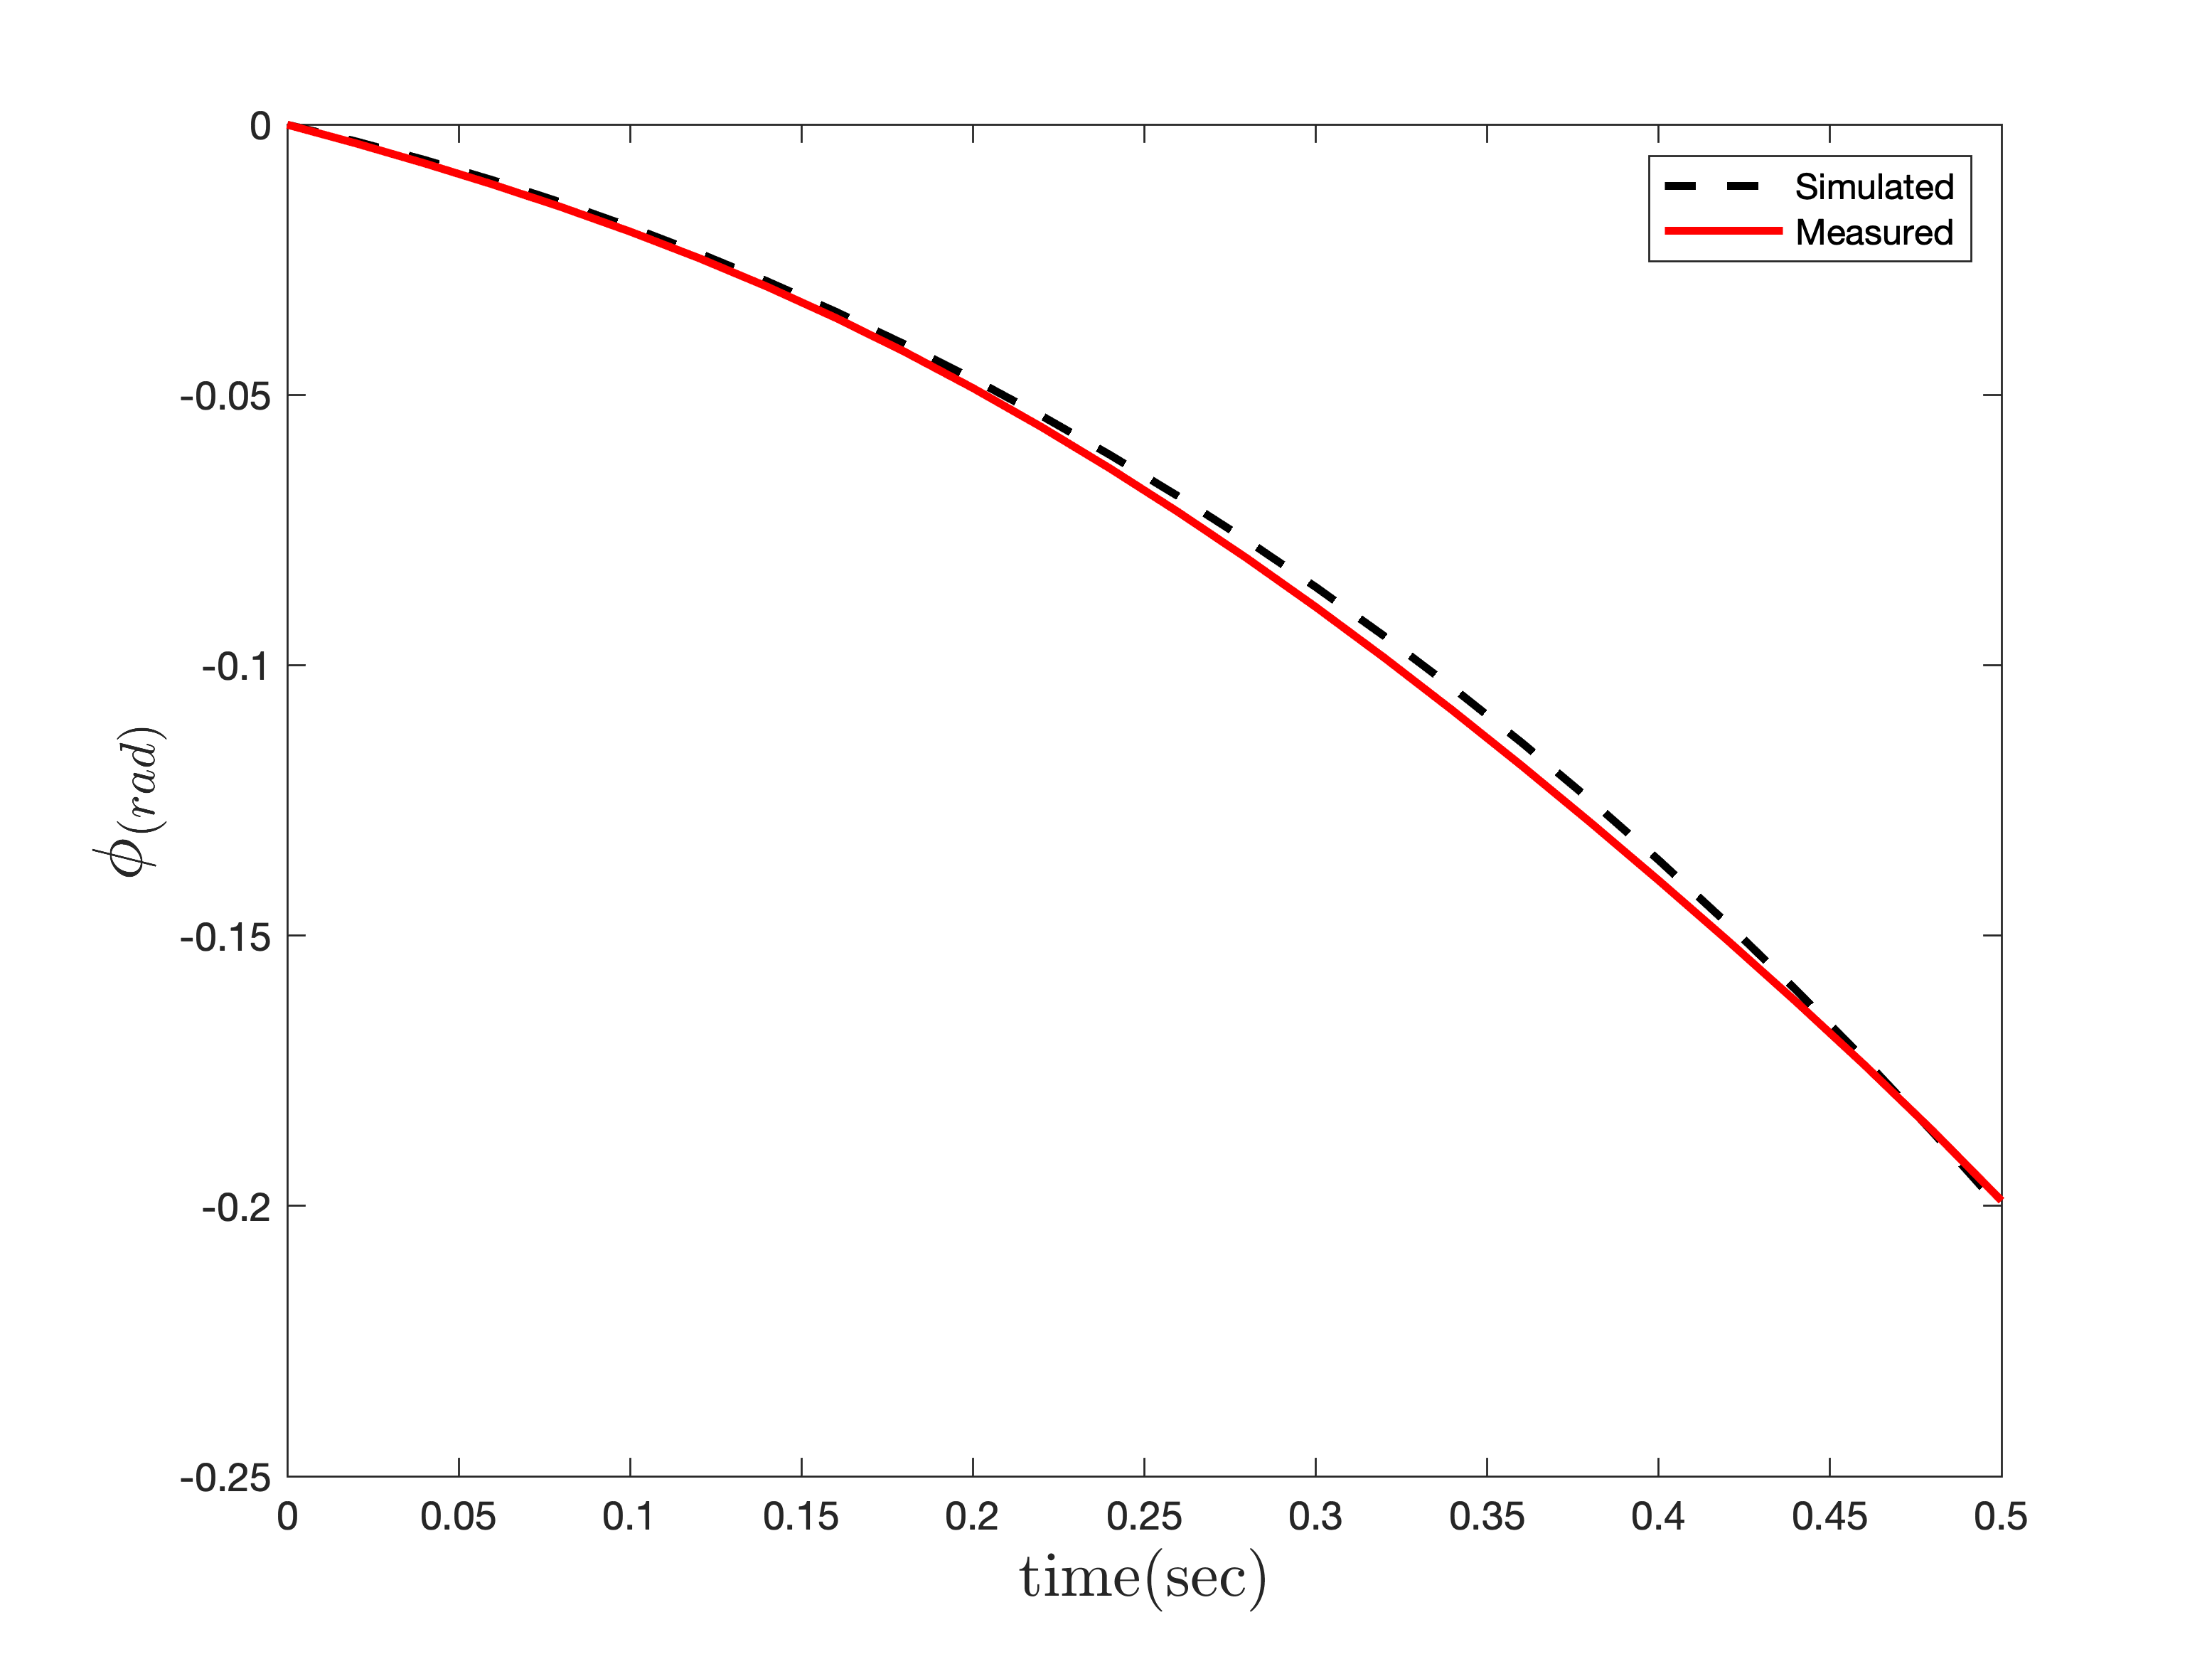
\includegraphics[width=1\linewidth]{../Figures/RCP/roll_ml_parameter_estimation/RCP_roll_S2.png}
		\captionof{figure}{مقايسه وضعیت کانال رول شبیه‌سازی و واقعیت}
	\end{minipage}
\end{minipage}
%%\subsection{تخمین پارامترهای کانال پیچ موتور خاموش}
%برای اصلاح پارامترهای پیچ چندین آزمایش انجام شد و با استفاده از داده‌های ثبت شده از وضعیت استند در کانال پیچ و جعبه‌ابزار
%\lr{Parameter Estimator}،
%پارامترهای کانال پیچ اصلاح شدند.
%برای انجام آزمایش استند از شرایط اولیه مختلف با موتور خاموش رها شد  و از خروجی سنسور داده برداری شد. سپس، مدل و داده‌های ثبت شده‌ی سنسور (وضعیت استند در کانال پیچ) به جعبه‌ابزار
%\lr{Parameter Estimator}
%داده‌شد. وضعیت کانال پیچ استند در شبیه‌سازی و واقعیت بعد از اصلاح پارامترهای کانال پیچ در شکل‌های
%\ref{pitch_ml_ps1}, \ref{pitch_ml_ps3} , \ref{pitch_ml_ps4}  و \ref{pitch_ml_ps5}
%مقایسه شده است.
%
%\begin{figure}[H]
%	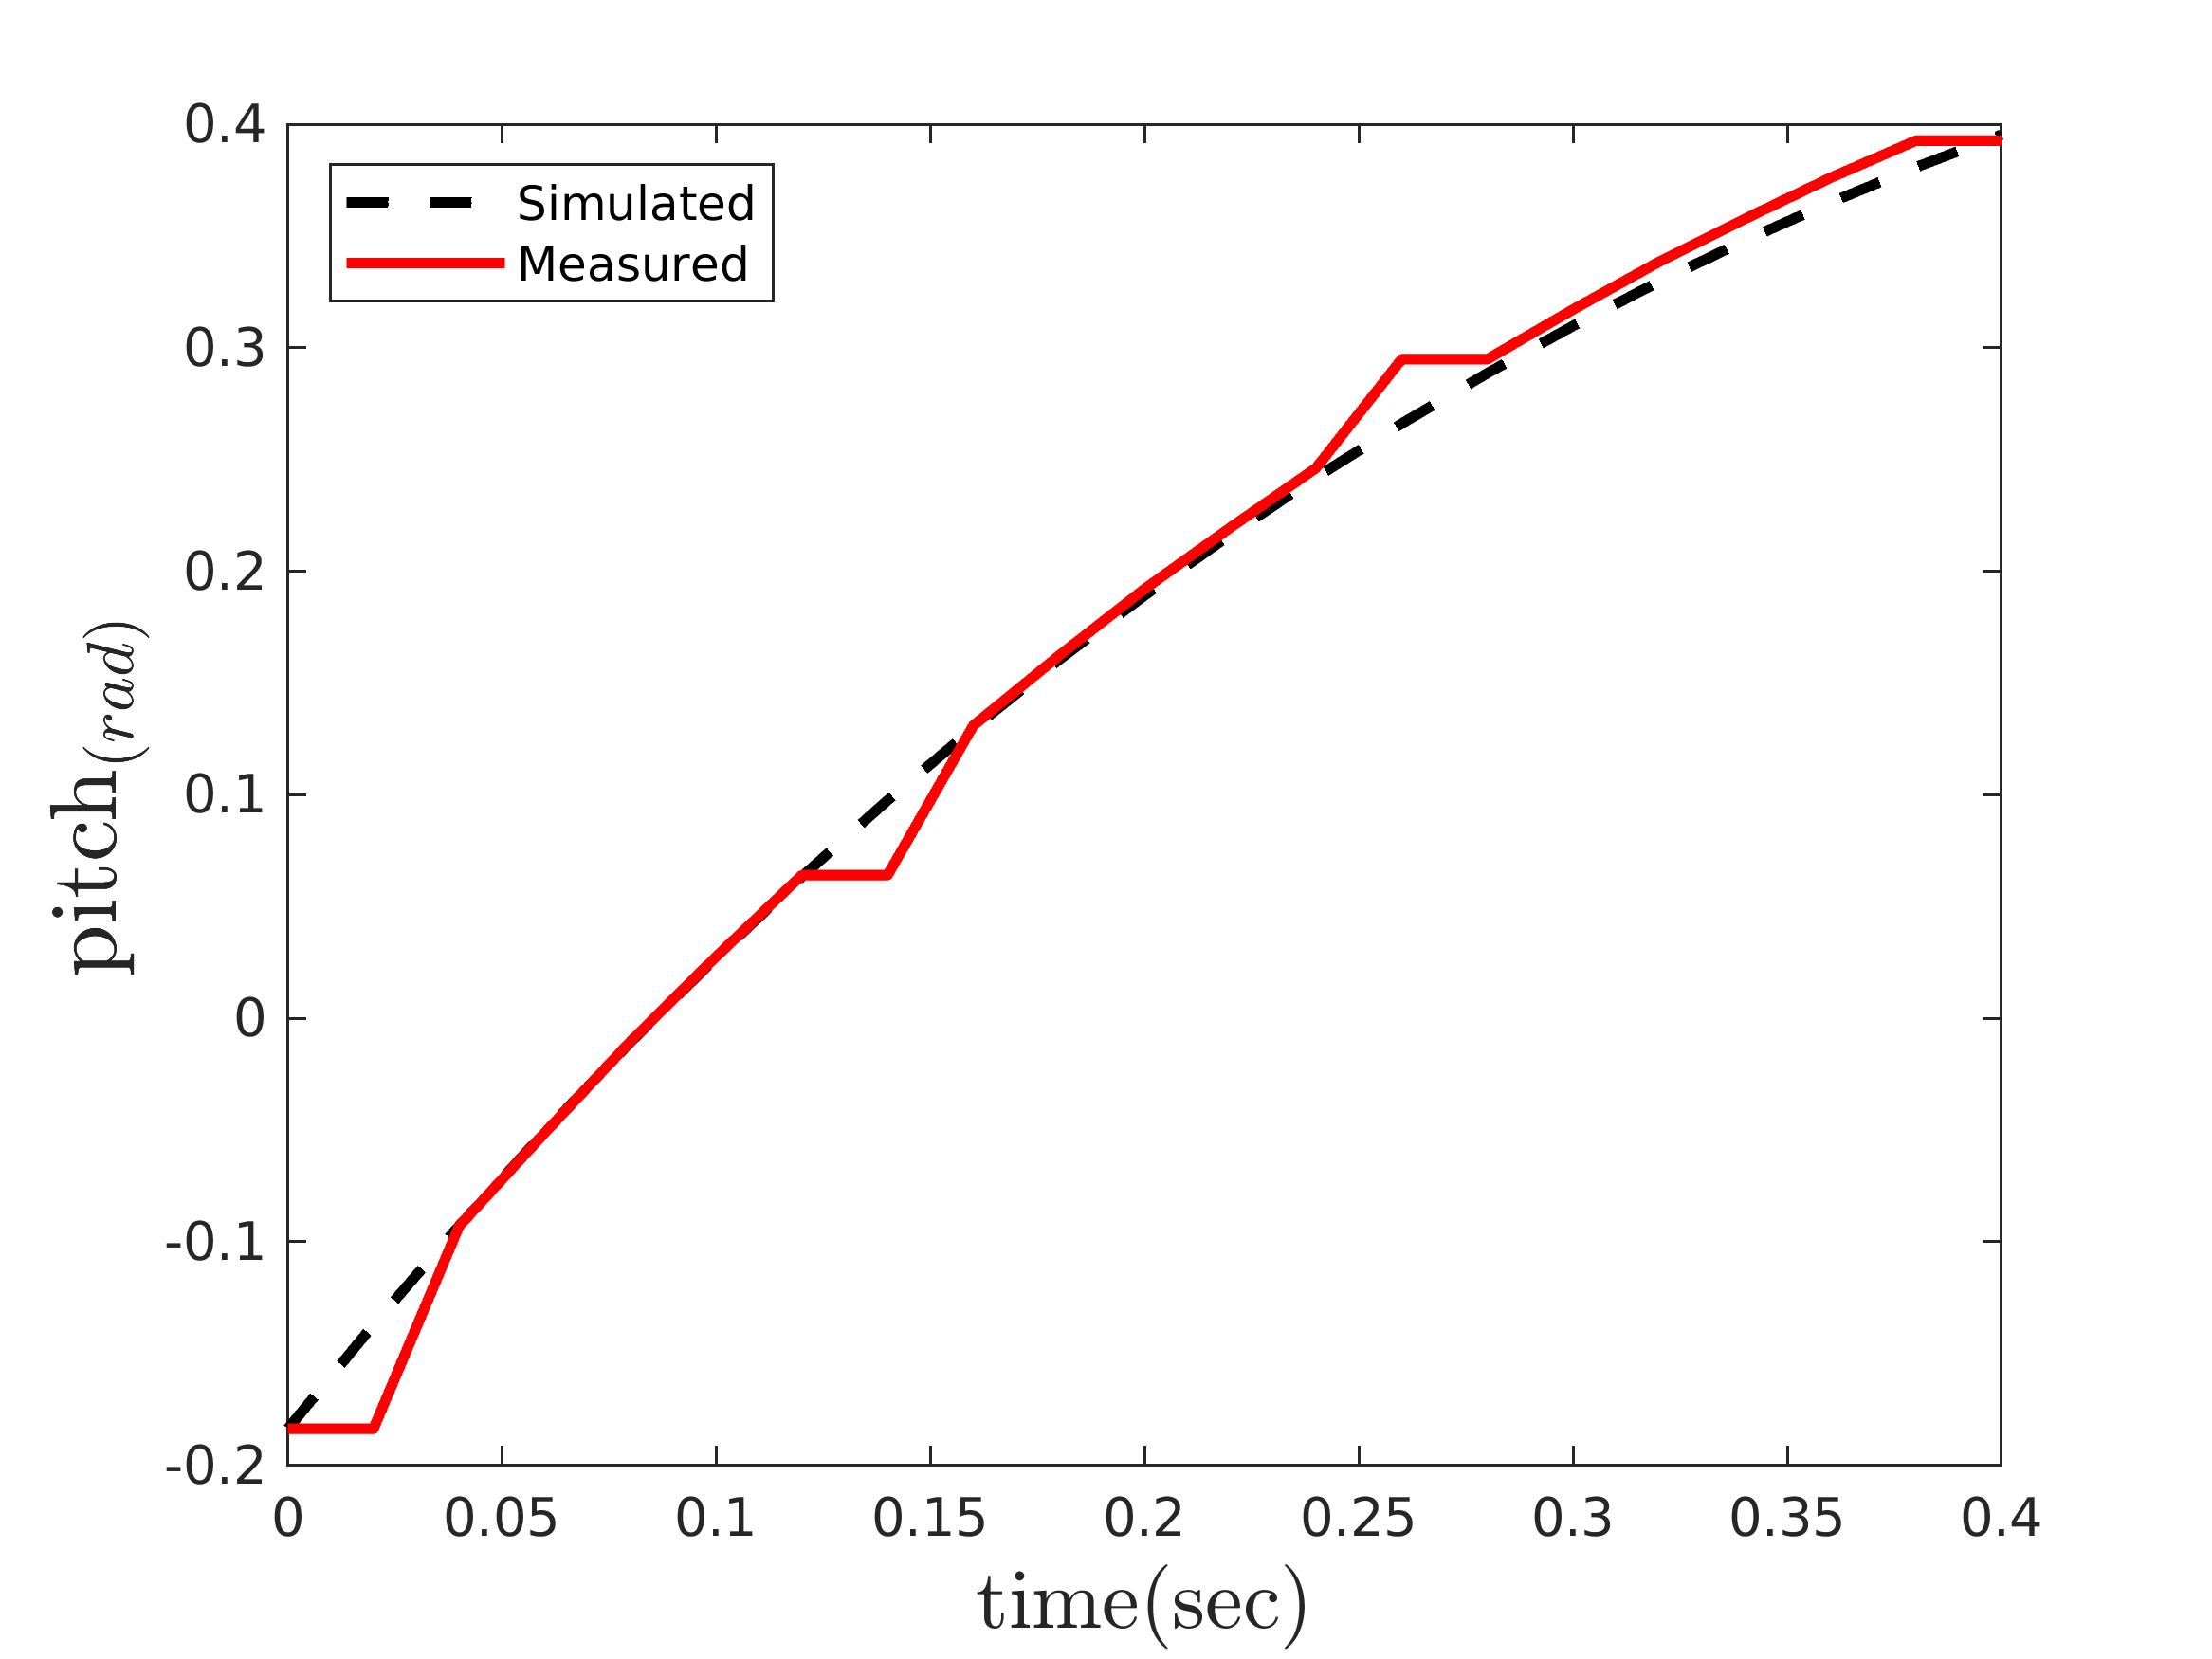
\includegraphics[width=.48\linewidth]{../Figures/RCP/pitch_ml_parameter_estimation/RCP_pitch_S1.png}
%	\centering
%	\caption{مقايسه وضعیت استند در  آزمايش اول و شبیه‌سازی، پس از تخمین پارامترهای کانال پیچ موتور خاموش}
%	\label{pitch_ml_ps1}
%\end{figure}
%\begin{figure}[H]
%	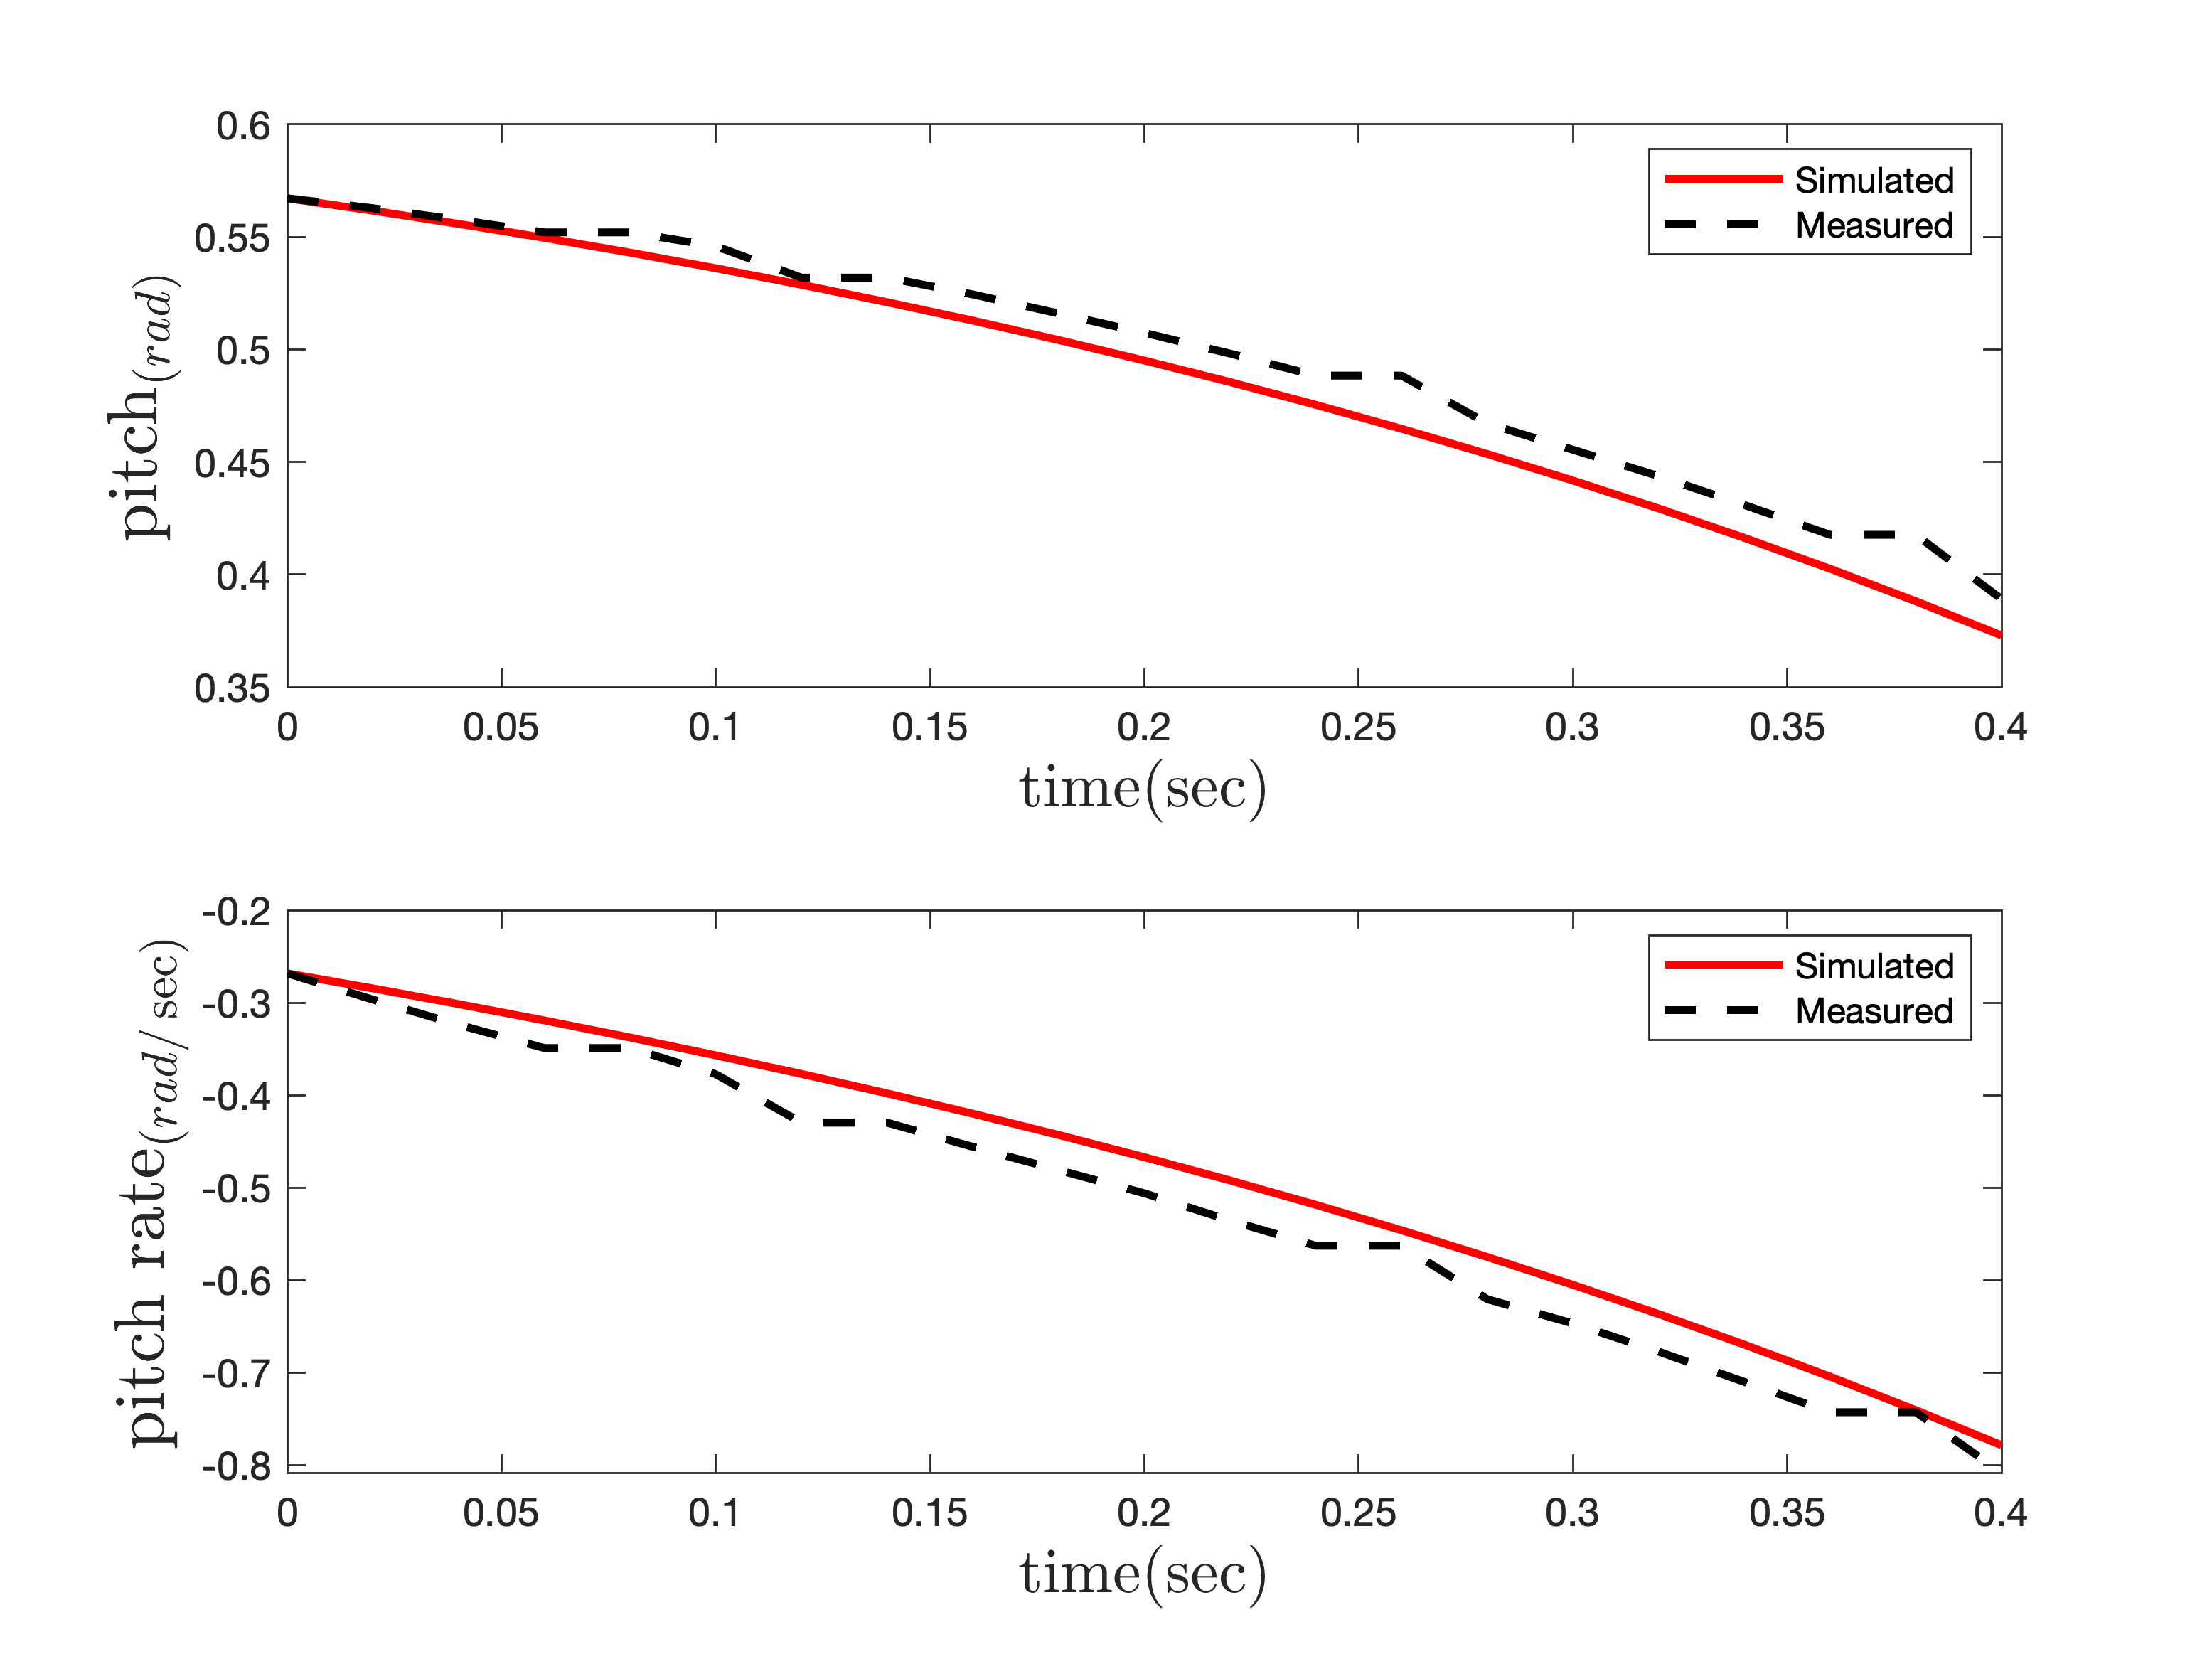
\includegraphics[width=12cm]{../Figures/RCP/pitch_ml_parameter_estimation/RCP_pitch_S2.png}
%	\centering
%	\caption{مقايسه وضعیت استند در  آزمايش دوم و شبیه‌سازی، پس از تخمین پارامترهای کانال پیچ موتور خاموش}
%	\label{pitch_ml_ps2}
%\end{figure}
%\begin{figure}[H]
%	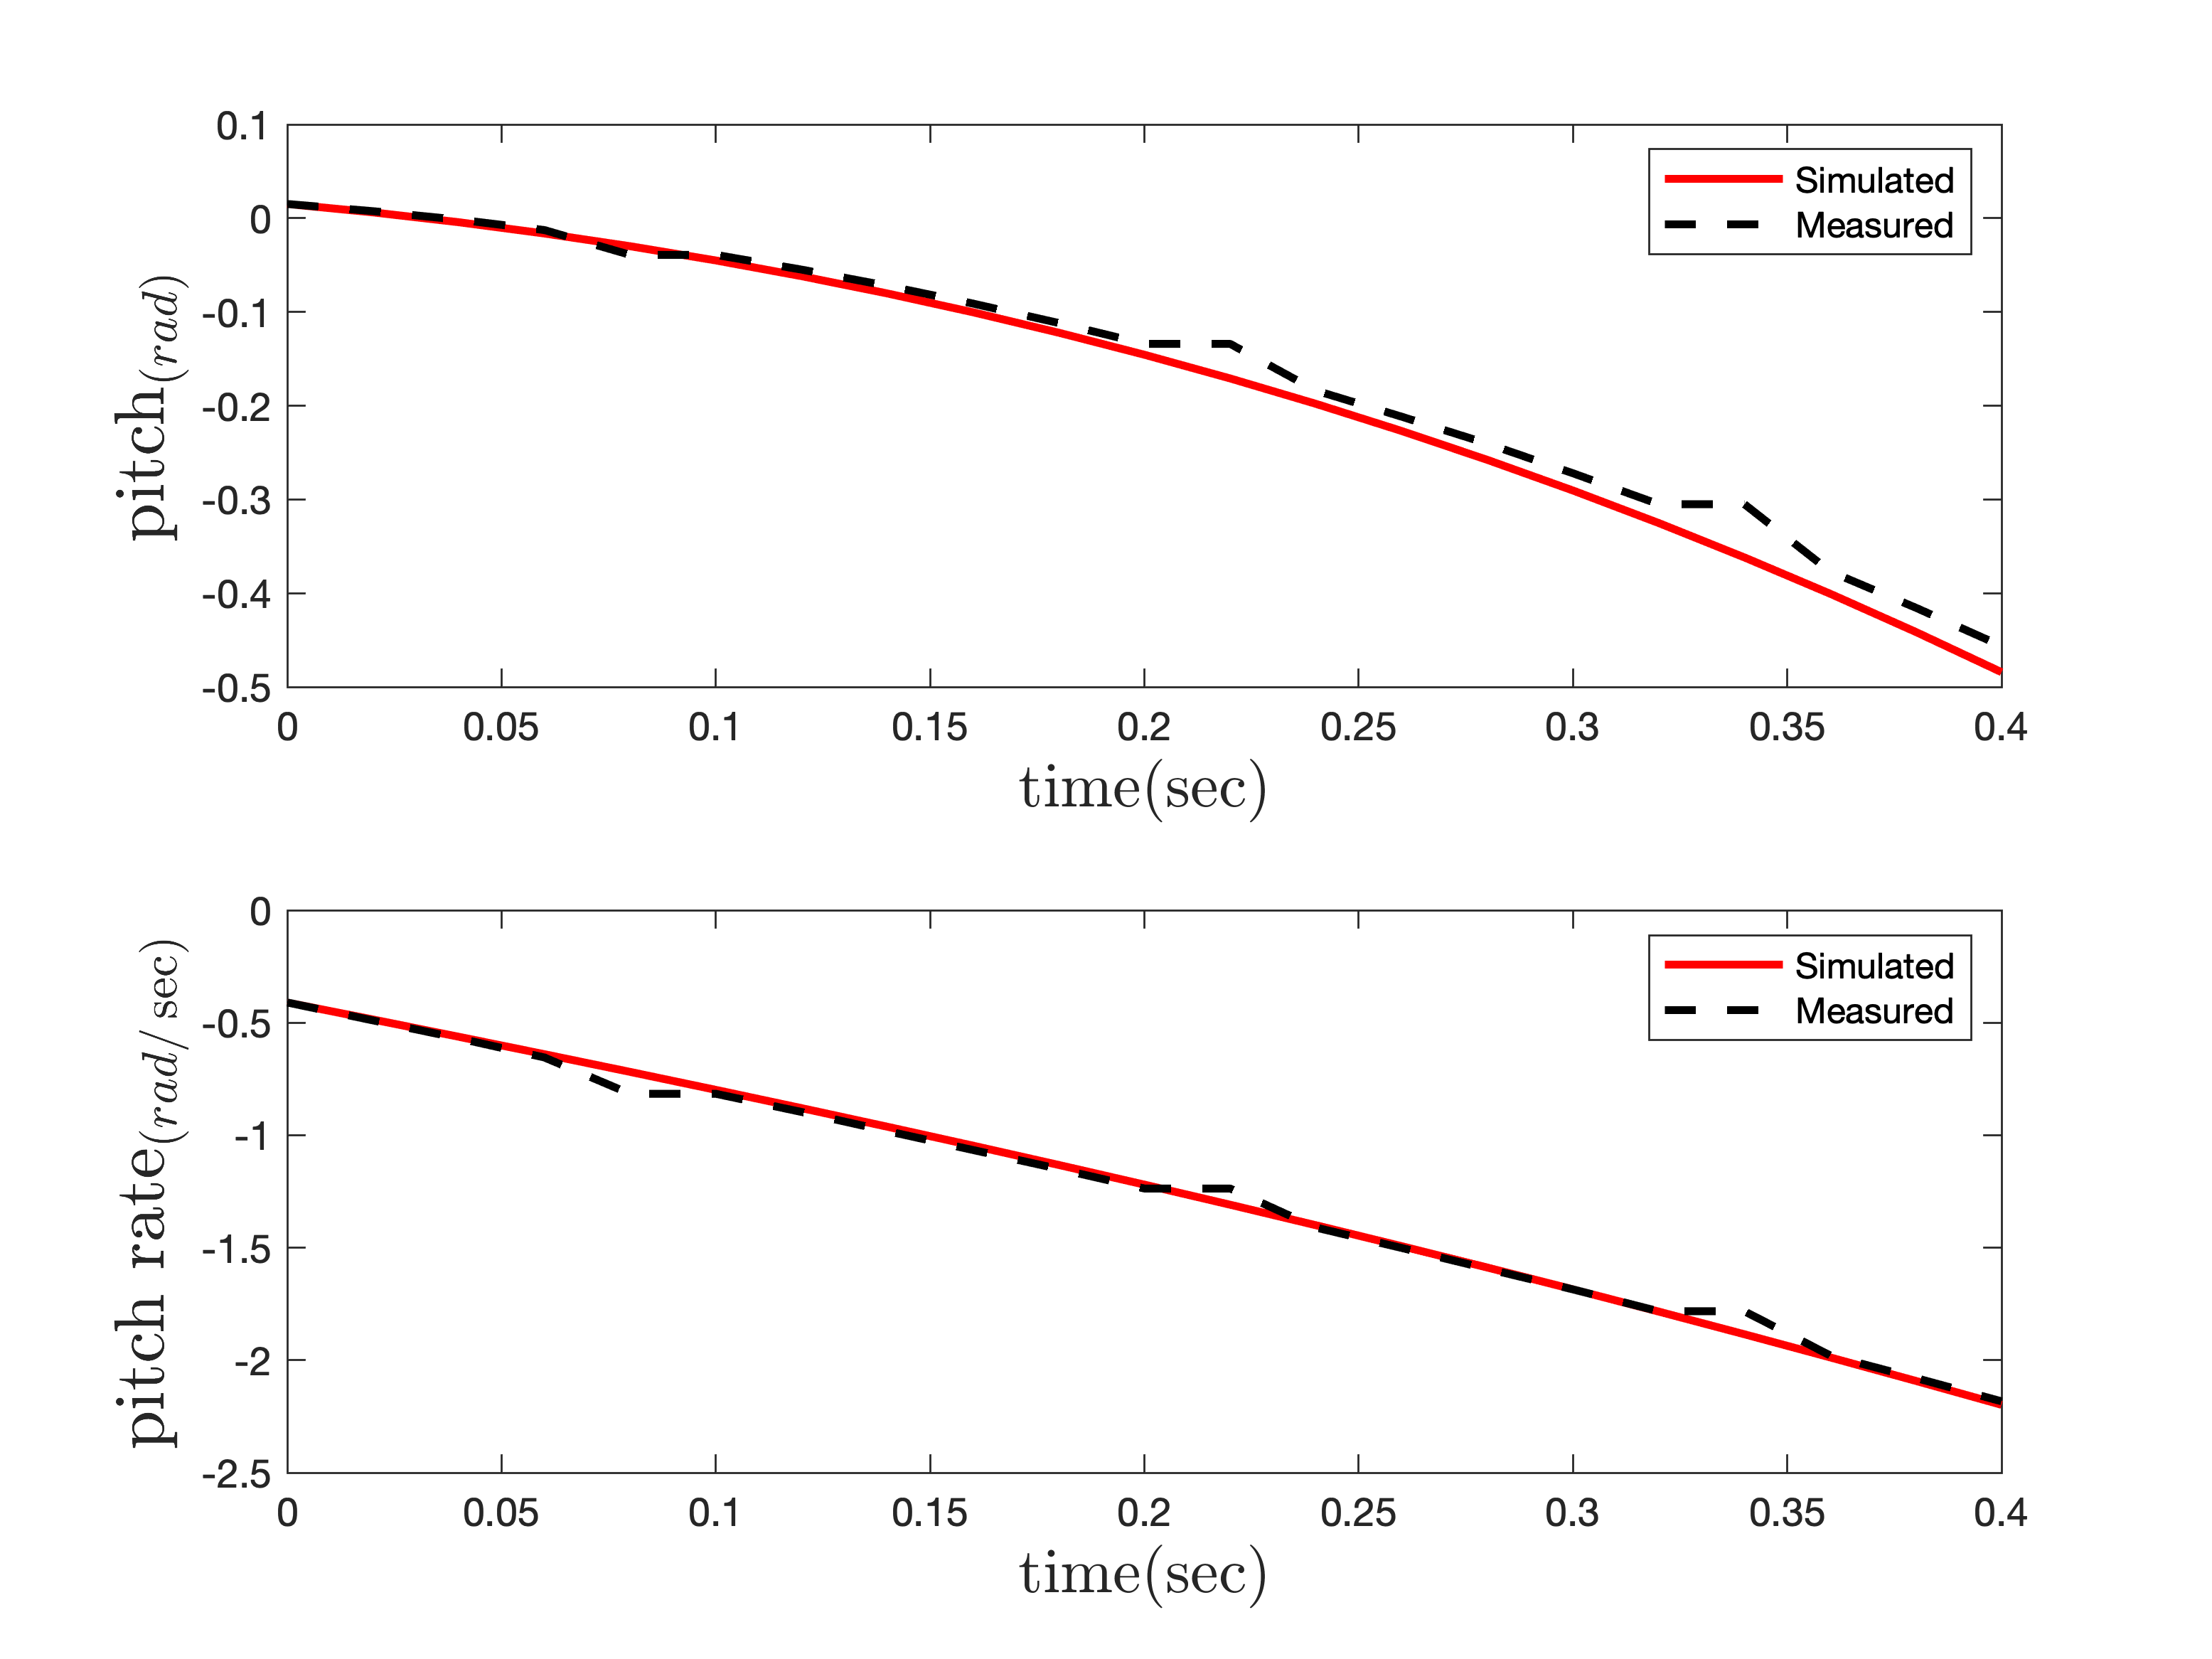
\includegraphics[width=12cm]{../Figures/RCP/pitch_ml_parameter_estimation/RCP_pitch_S3.png}
%	\centering
%	\caption{مقايسه وضعیت استند در  آزمايش سوم و شبیه‌سازی، پس از تخمین پارامترهای کانال پیچ موتور خاموش}
%	\label{pitch_ml_ps3}
%\end{figure}
%\begin{figure}[H]
%	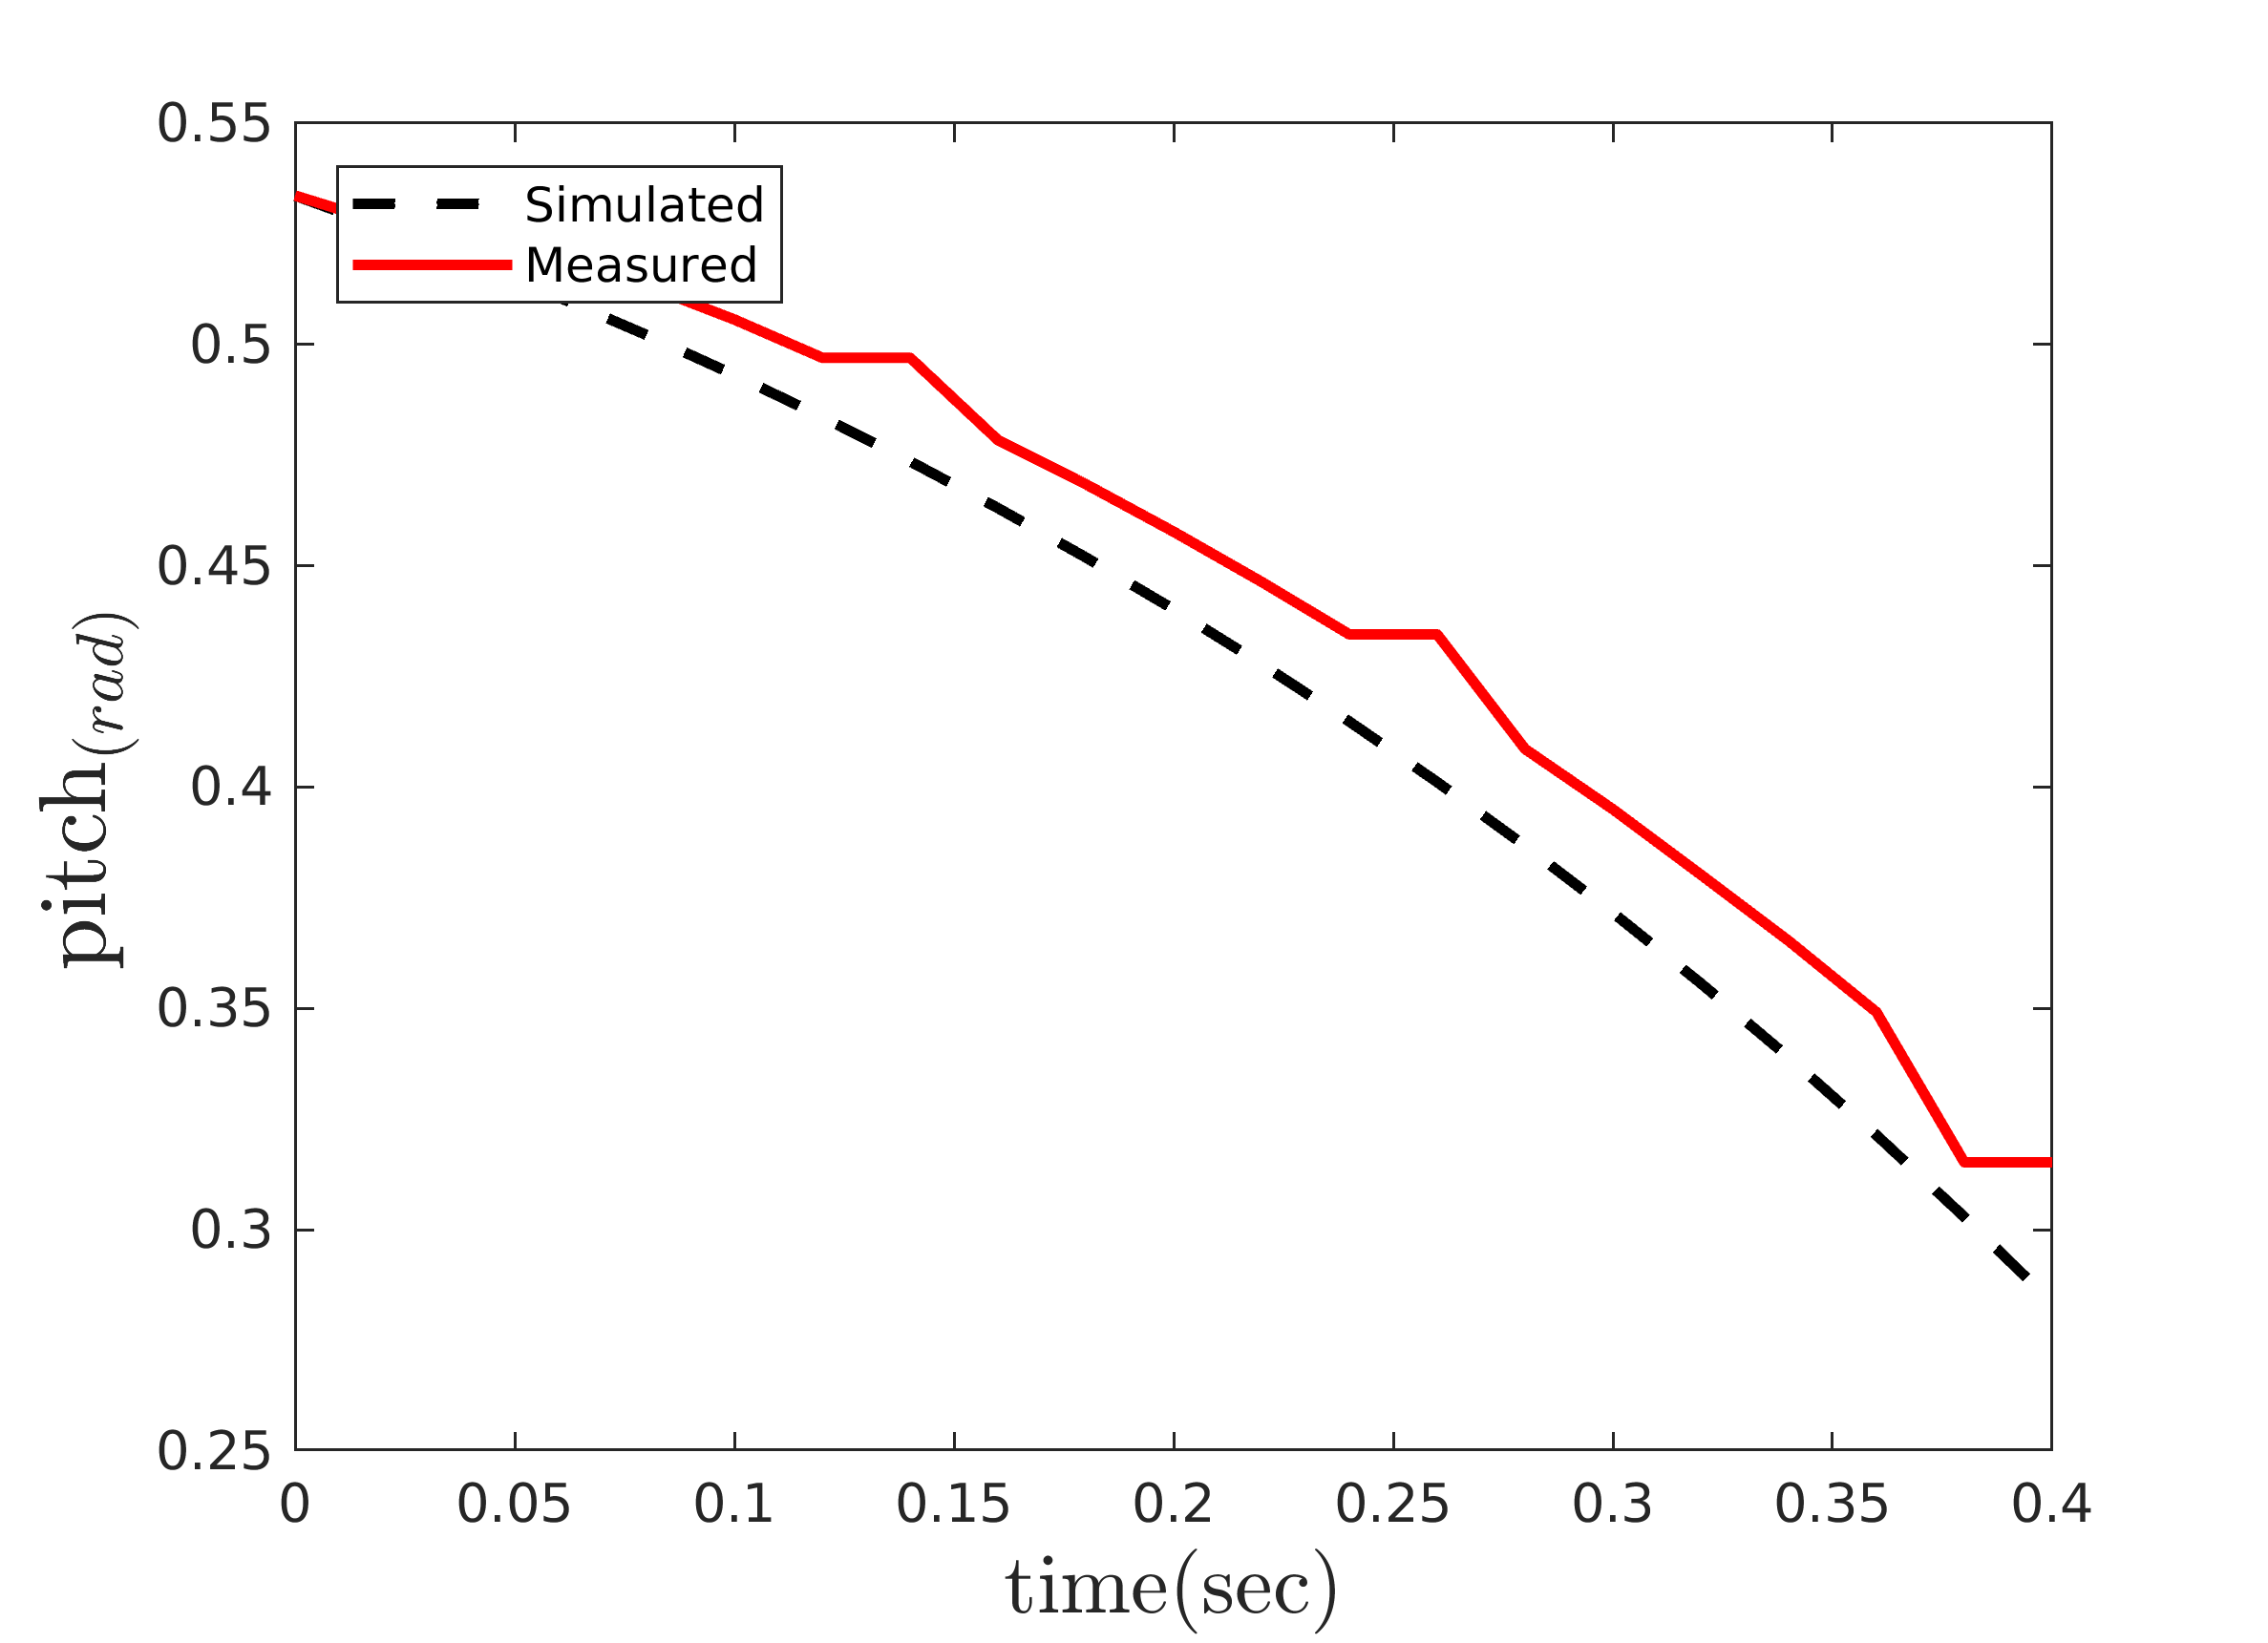
\includegraphics[width=12cm]{../Figures/RCP/pitch_ml_parameter_estimation/RCP_pitch_S4.png}
%	\centering
%	\caption{مقايسه وضعیت استند در  آزمايش چهارم و شبیه‌سازی، پس از تخمین پارامترهای کانال پیچ موتور خاموش}
%	\label{pitch_ml_ps4}
%\end{figure}
%\begin{figure}[H]
%	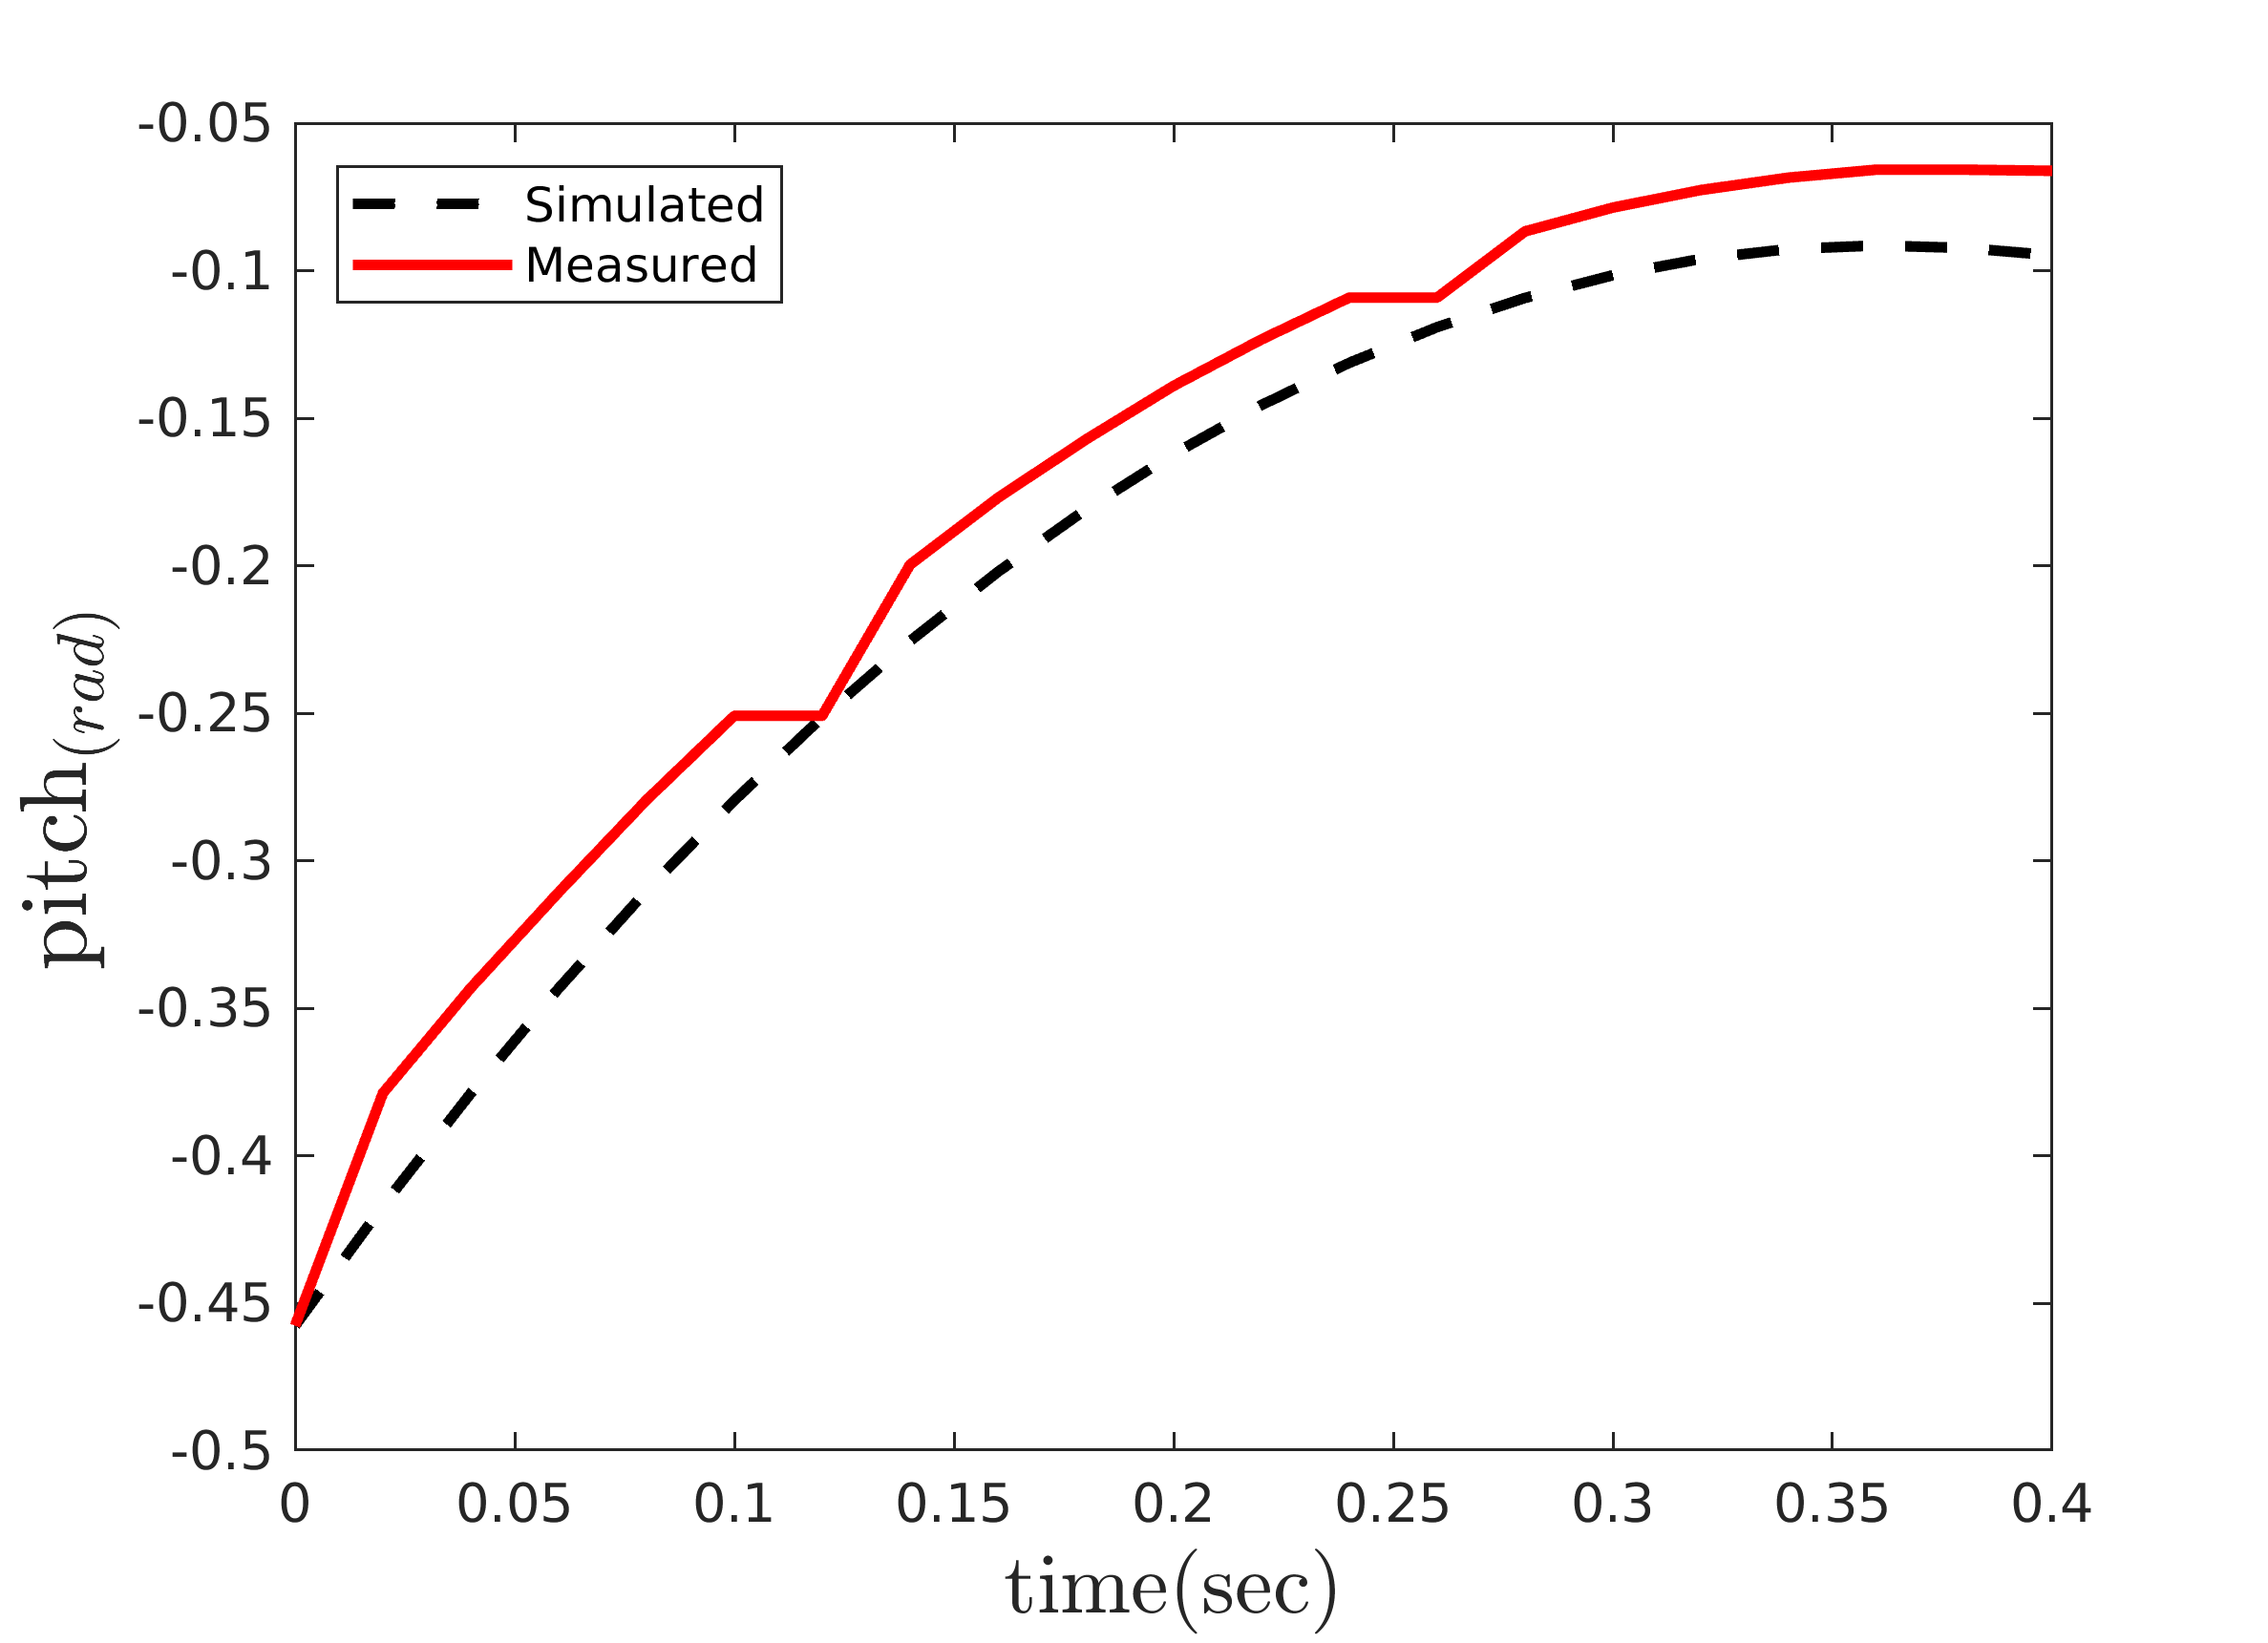
\includegraphics[width=12cm]{../Figures/RCP/pitch_ml_parameter_estimation/RCP_pitch_S5.png}
%	\centering
%	\caption{مقايسه وضعیت استند در  آزمايش پنجم و شبیه‌سازی، پس از تخمین پارامترهای کانال پیچ موتور خاموش}
%	\label{pitch_ml_ps5}
%\end{figure}
در ابتدا خروجی اصلاح پارامترهای کانال پیچ  حالت موتور خاموش و سپس حالت کلی آورده شده‌است.

  \begin{minipage}[H]{\linewidth}
	\hfill
	\begin{minipage}[b]{0.49\linewidth}
		\centering
		\begin{tabular}{ccc}\hline
			پارامتر & مقدار پارامتر  & مقدار پارامتر بعد از اصلاح
			\\ \hline
			$B_1$  & $4.53$ & $4.36$ \\
			$B_5$ & $0.007$ & $0.012$\\
			$B_6$ & $4.13$ & $4.428$\\\\\\
		\end{tabular}
		\captionof{table}{مقايسه پارامترهای کانال پیچ قبل و بعد از اصلاح}
	\end{minipage}
	\begin{minipage}[b]{0.48\linewidth}
		\centering
		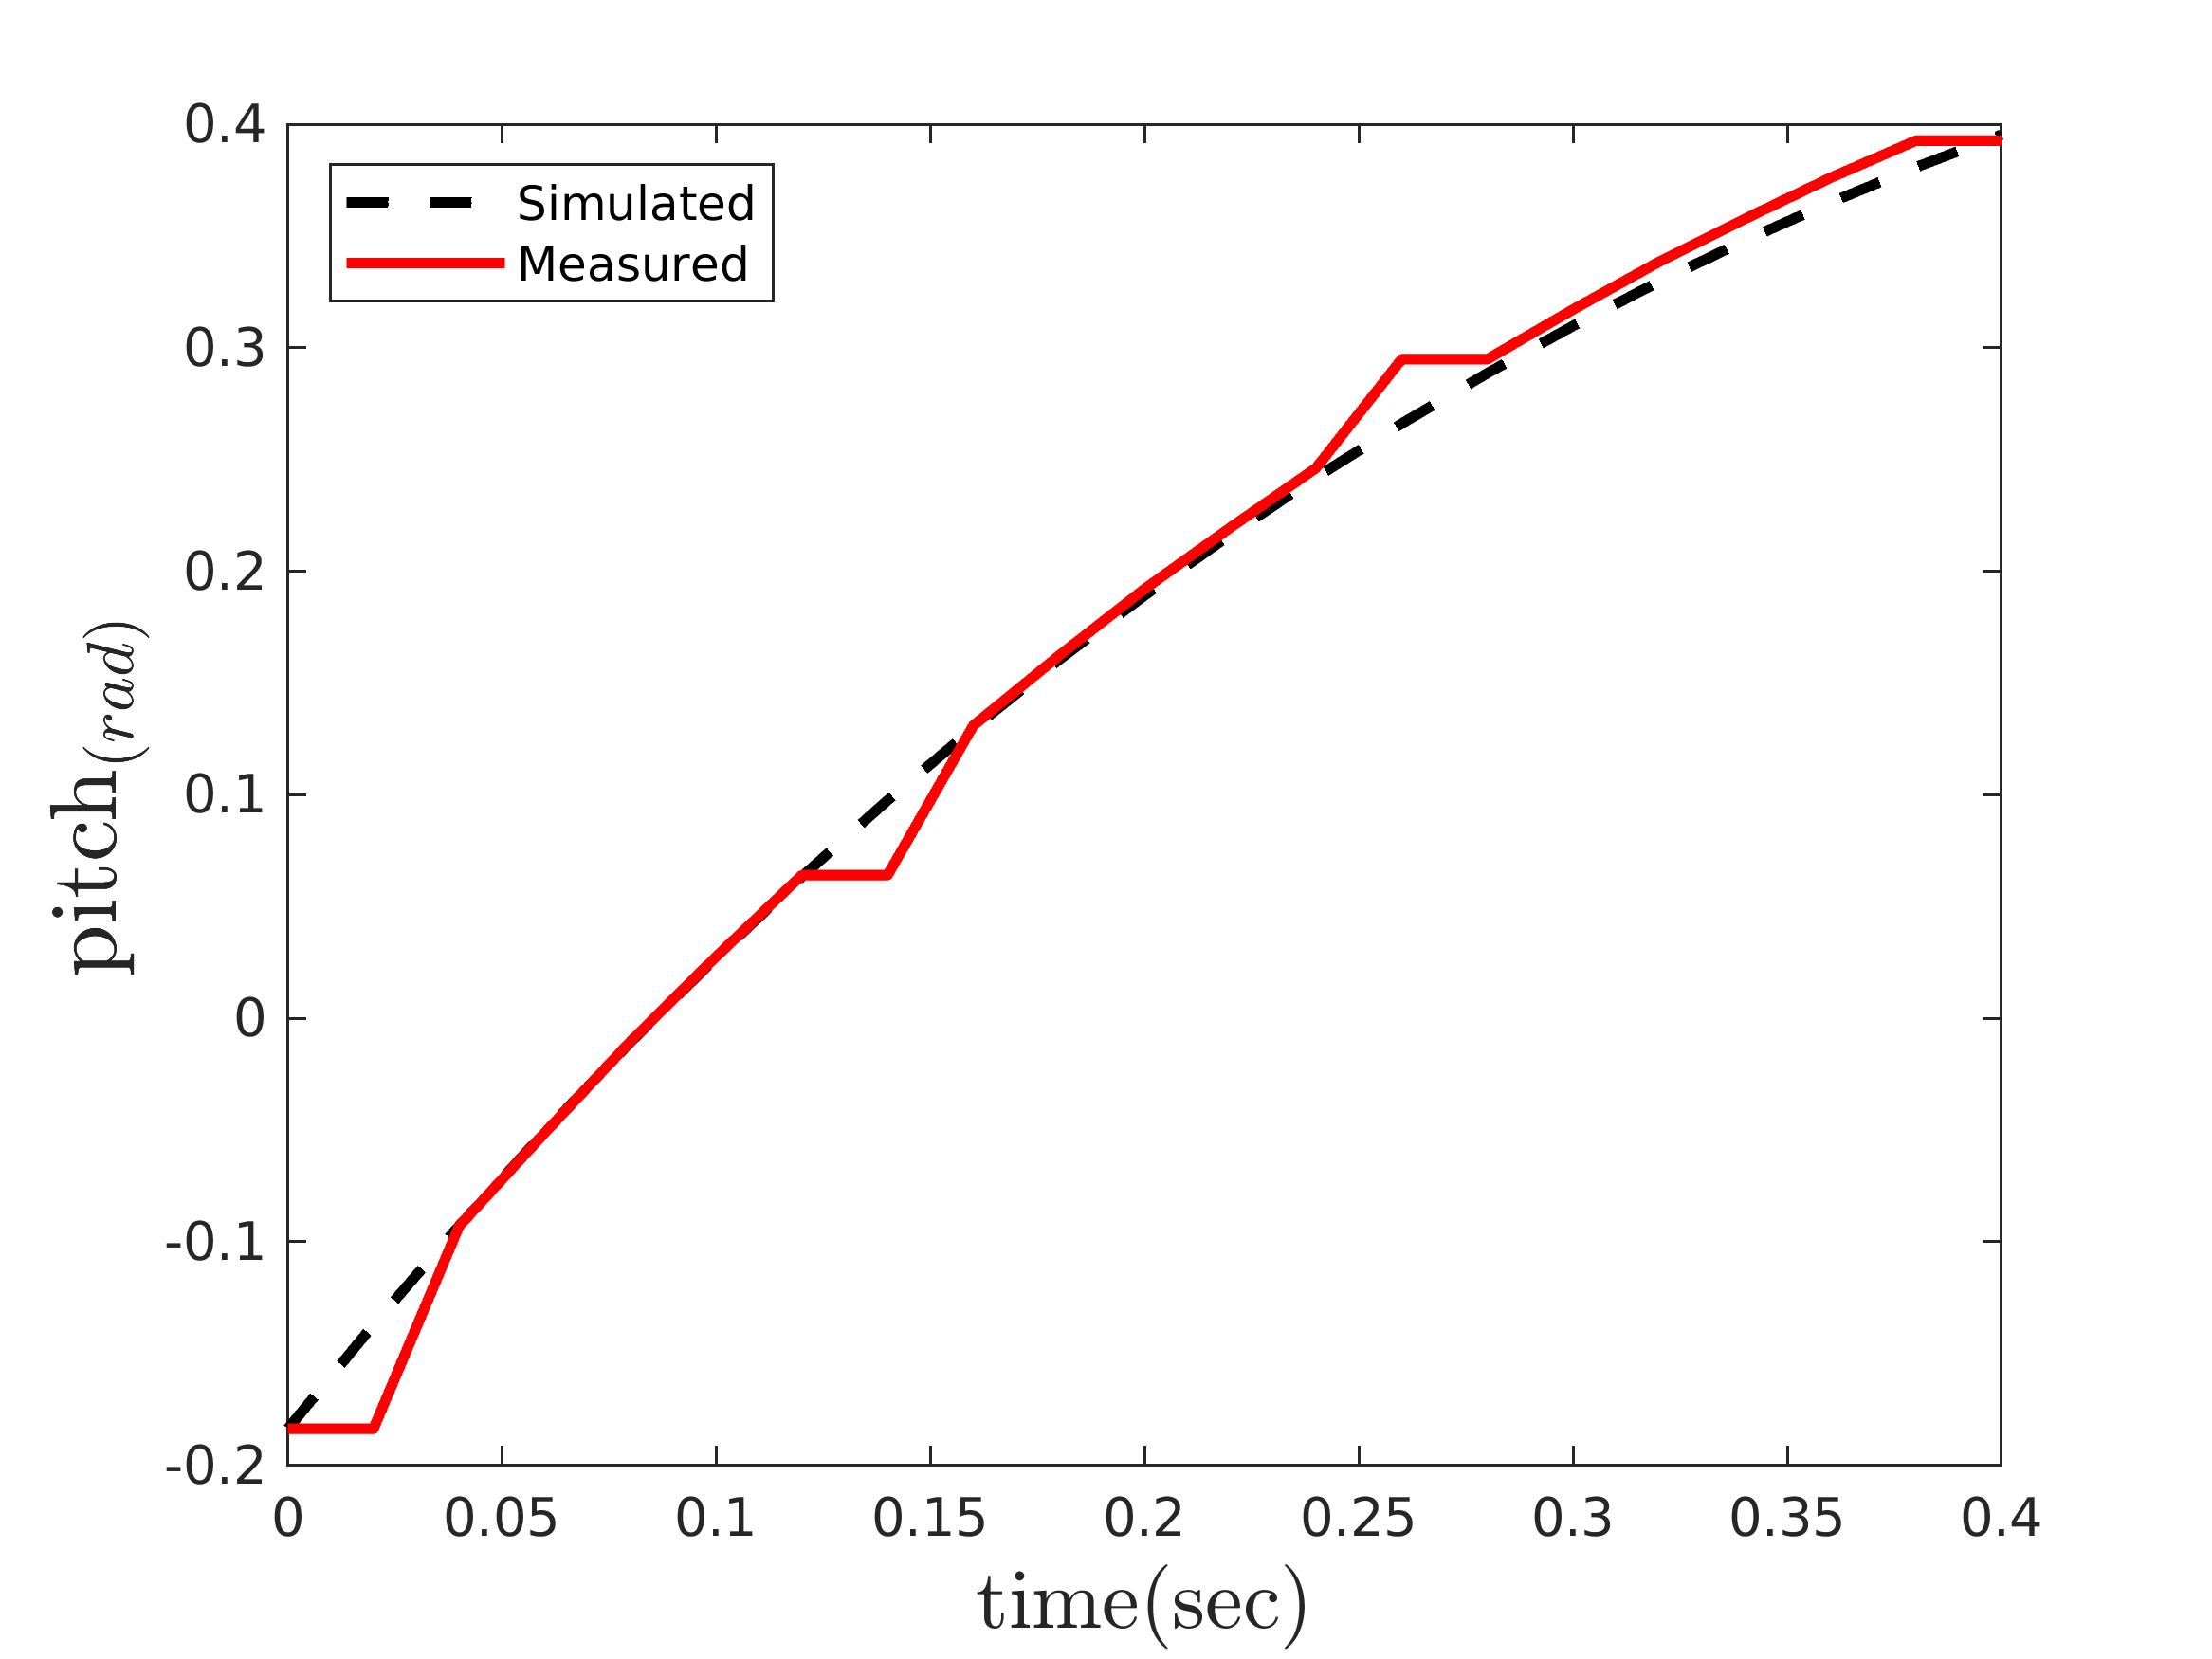
\includegraphics[width=1\linewidth]{../Figures/RCP/pitch_ml_parameter_estimation/RCP_pitch_S1.png}
		\captionof{figure}{مقايسه وضعیت کانال پیچ در شبیه‌سازی و واقعیت}
	\end{minipage}
\end{minipage}


%\subsection{تخمین پارامترهای کانال پپچ}
برای اصلاح پارامترهای پپچ چندین آزمایش انجام شد و با استفاده از داده‌های ثبت شده از وضعیت استند در کانال پپچ و جعبه‌ابزار
\lr{Parameter Estimator}،
پارامترهای کانال پپچ اصلاح شدند.
برای انجام آزمایش هر یک از موتورهای دو و چهار  با دور مختلف شروع به حرکت کردند و از خروجی سنسور داده برداری شد. سپس، مدل و داده‌های ثبت شده‌ی سنسور (وضعیت استند در کانال پپچ) به جعبه‌ابزار
\lr{Parameter Estimator}
داده شد. وضعیت کانال پپچ استند در شبیه‌سازی و واقعیت بعد از اصلاح پارامترهای کانال پپچ در شکل‌های
\ref{pitch_ps1}, \ref{pitch_ps2}, و \ref{pitch_ps3}
مقایسه شده است.

\begin{figure}[H]
	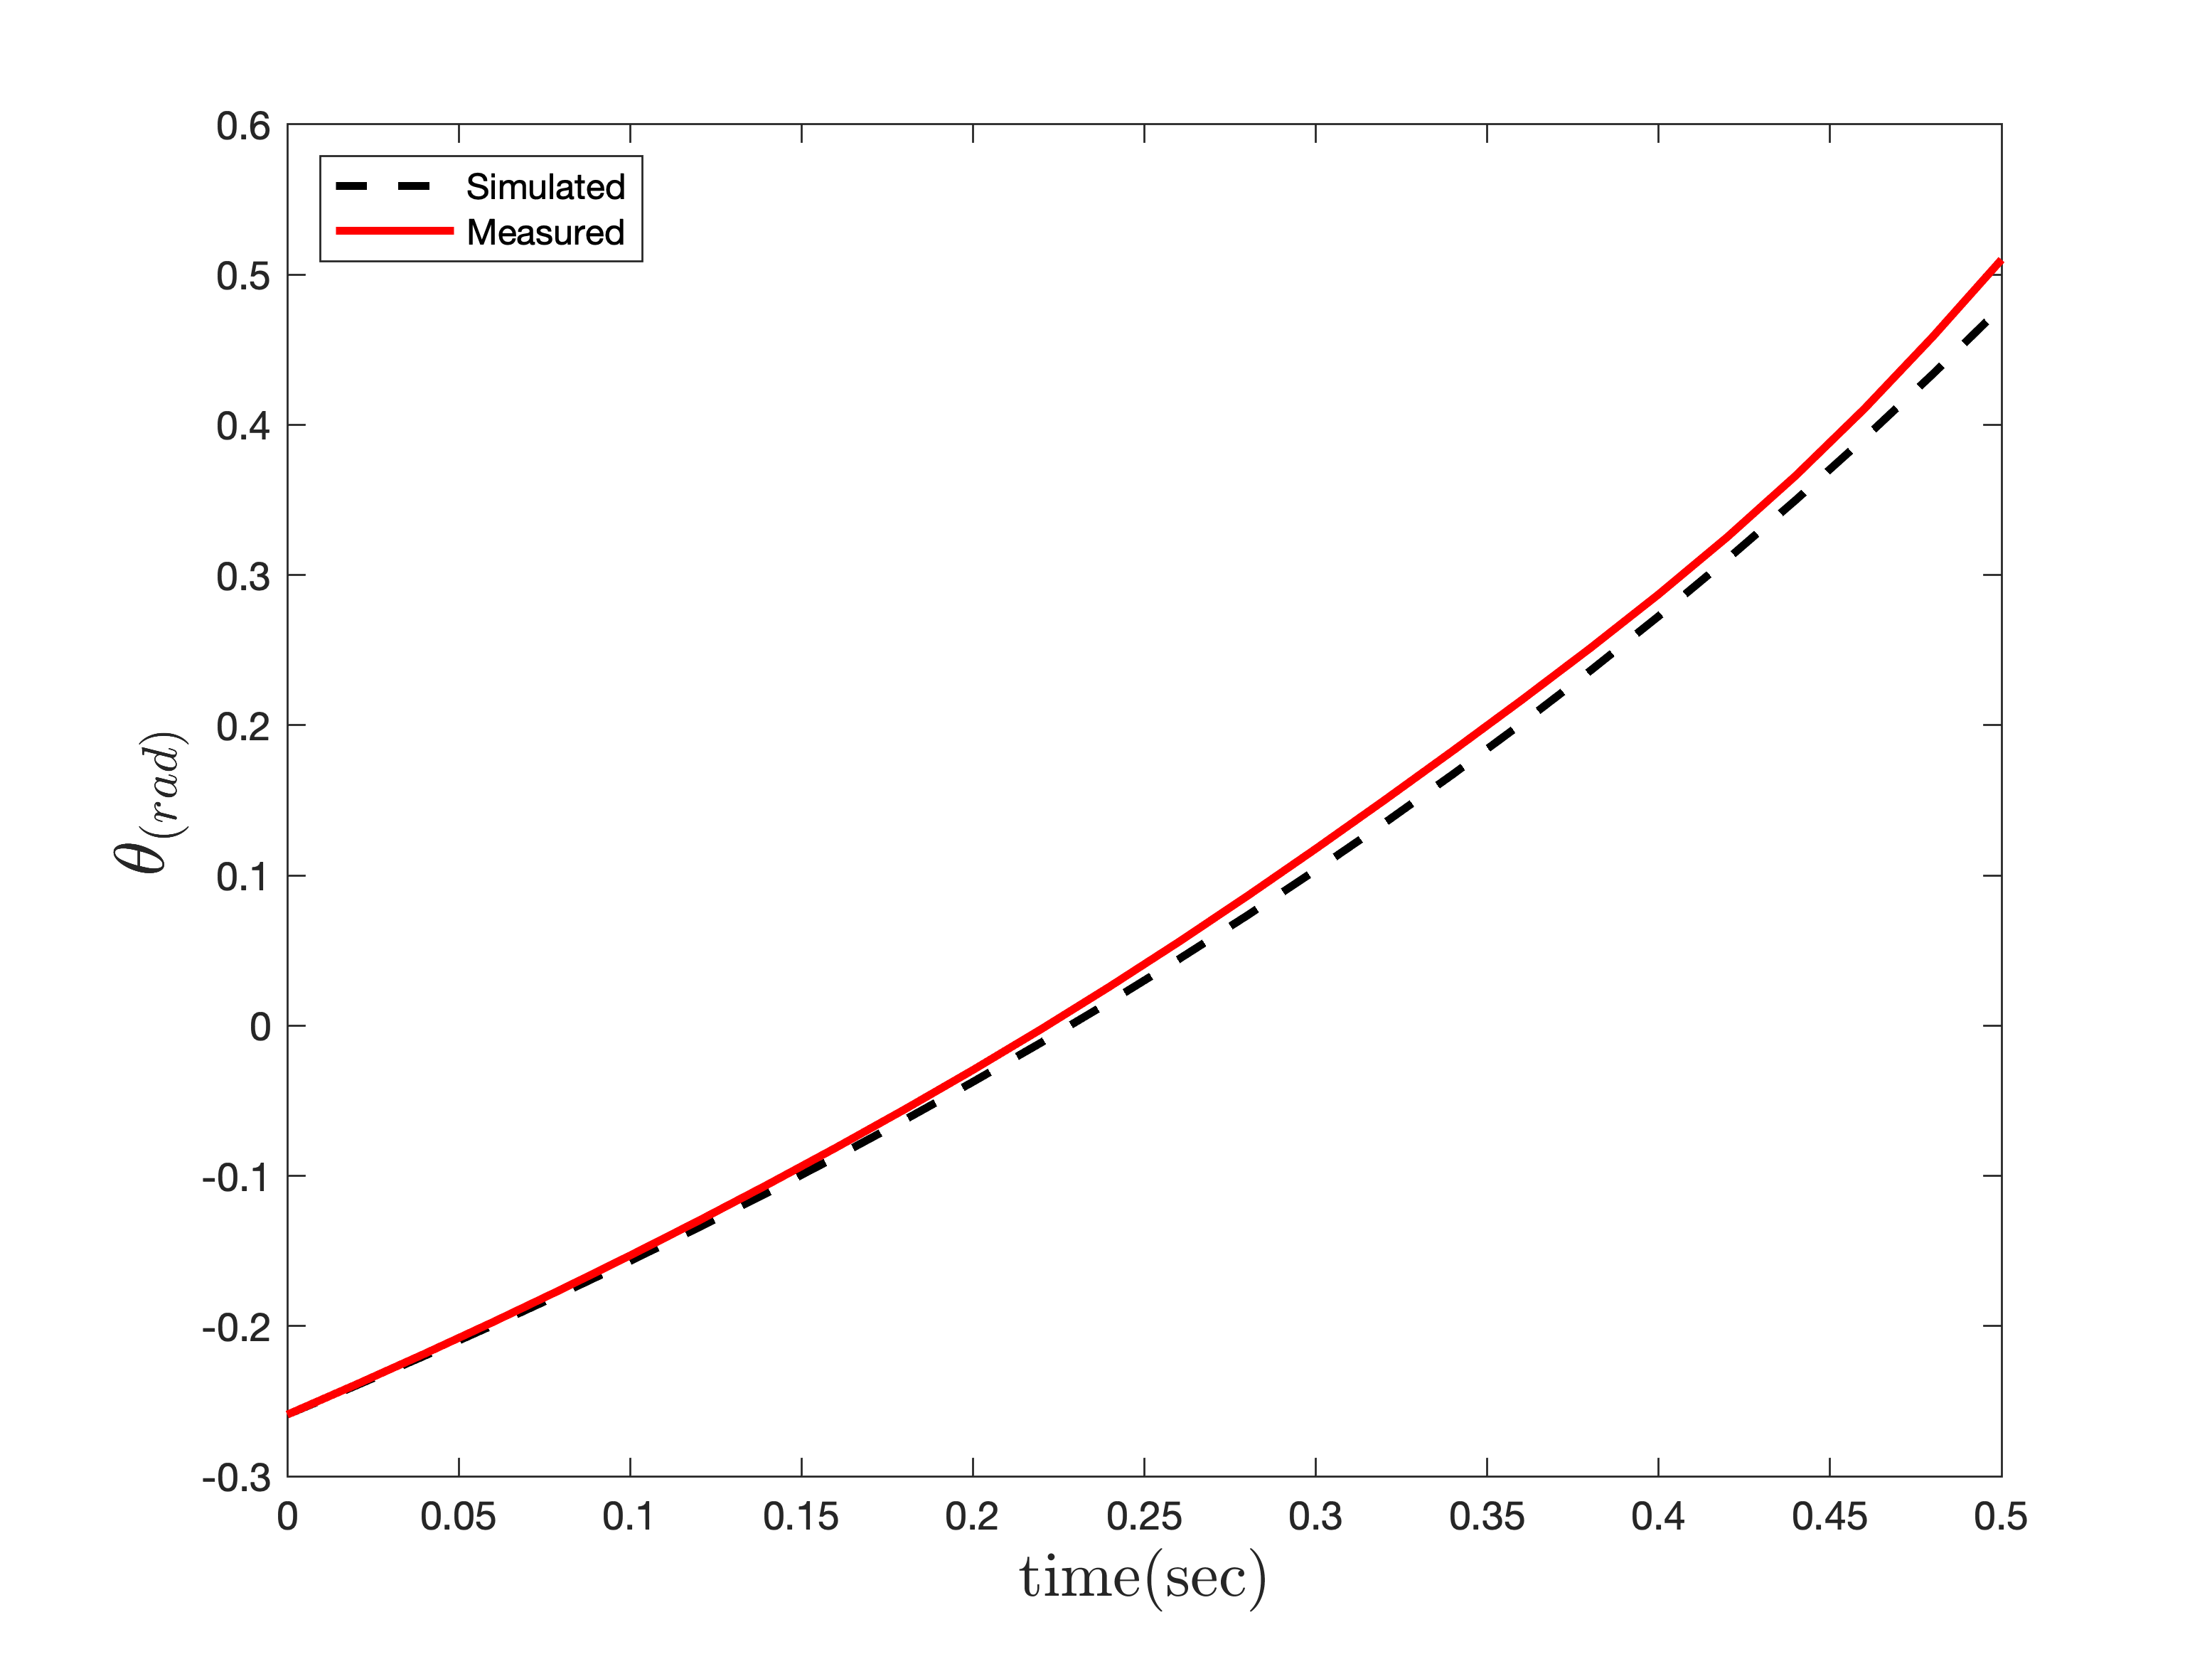
\includegraphics[width=12cm]{../Figures/RCP/pitch_parameter_estimation/RCP_pitch_S1.png}
	\centering
	\caption{مقايسه وضعیت استند در  آزمايش اول و شبیه‌سازی، پس از تخمین پارامترهای کانال پپچ}
	\label{pitch_ps1}
\end{figure}
\begin{figure}[H]
	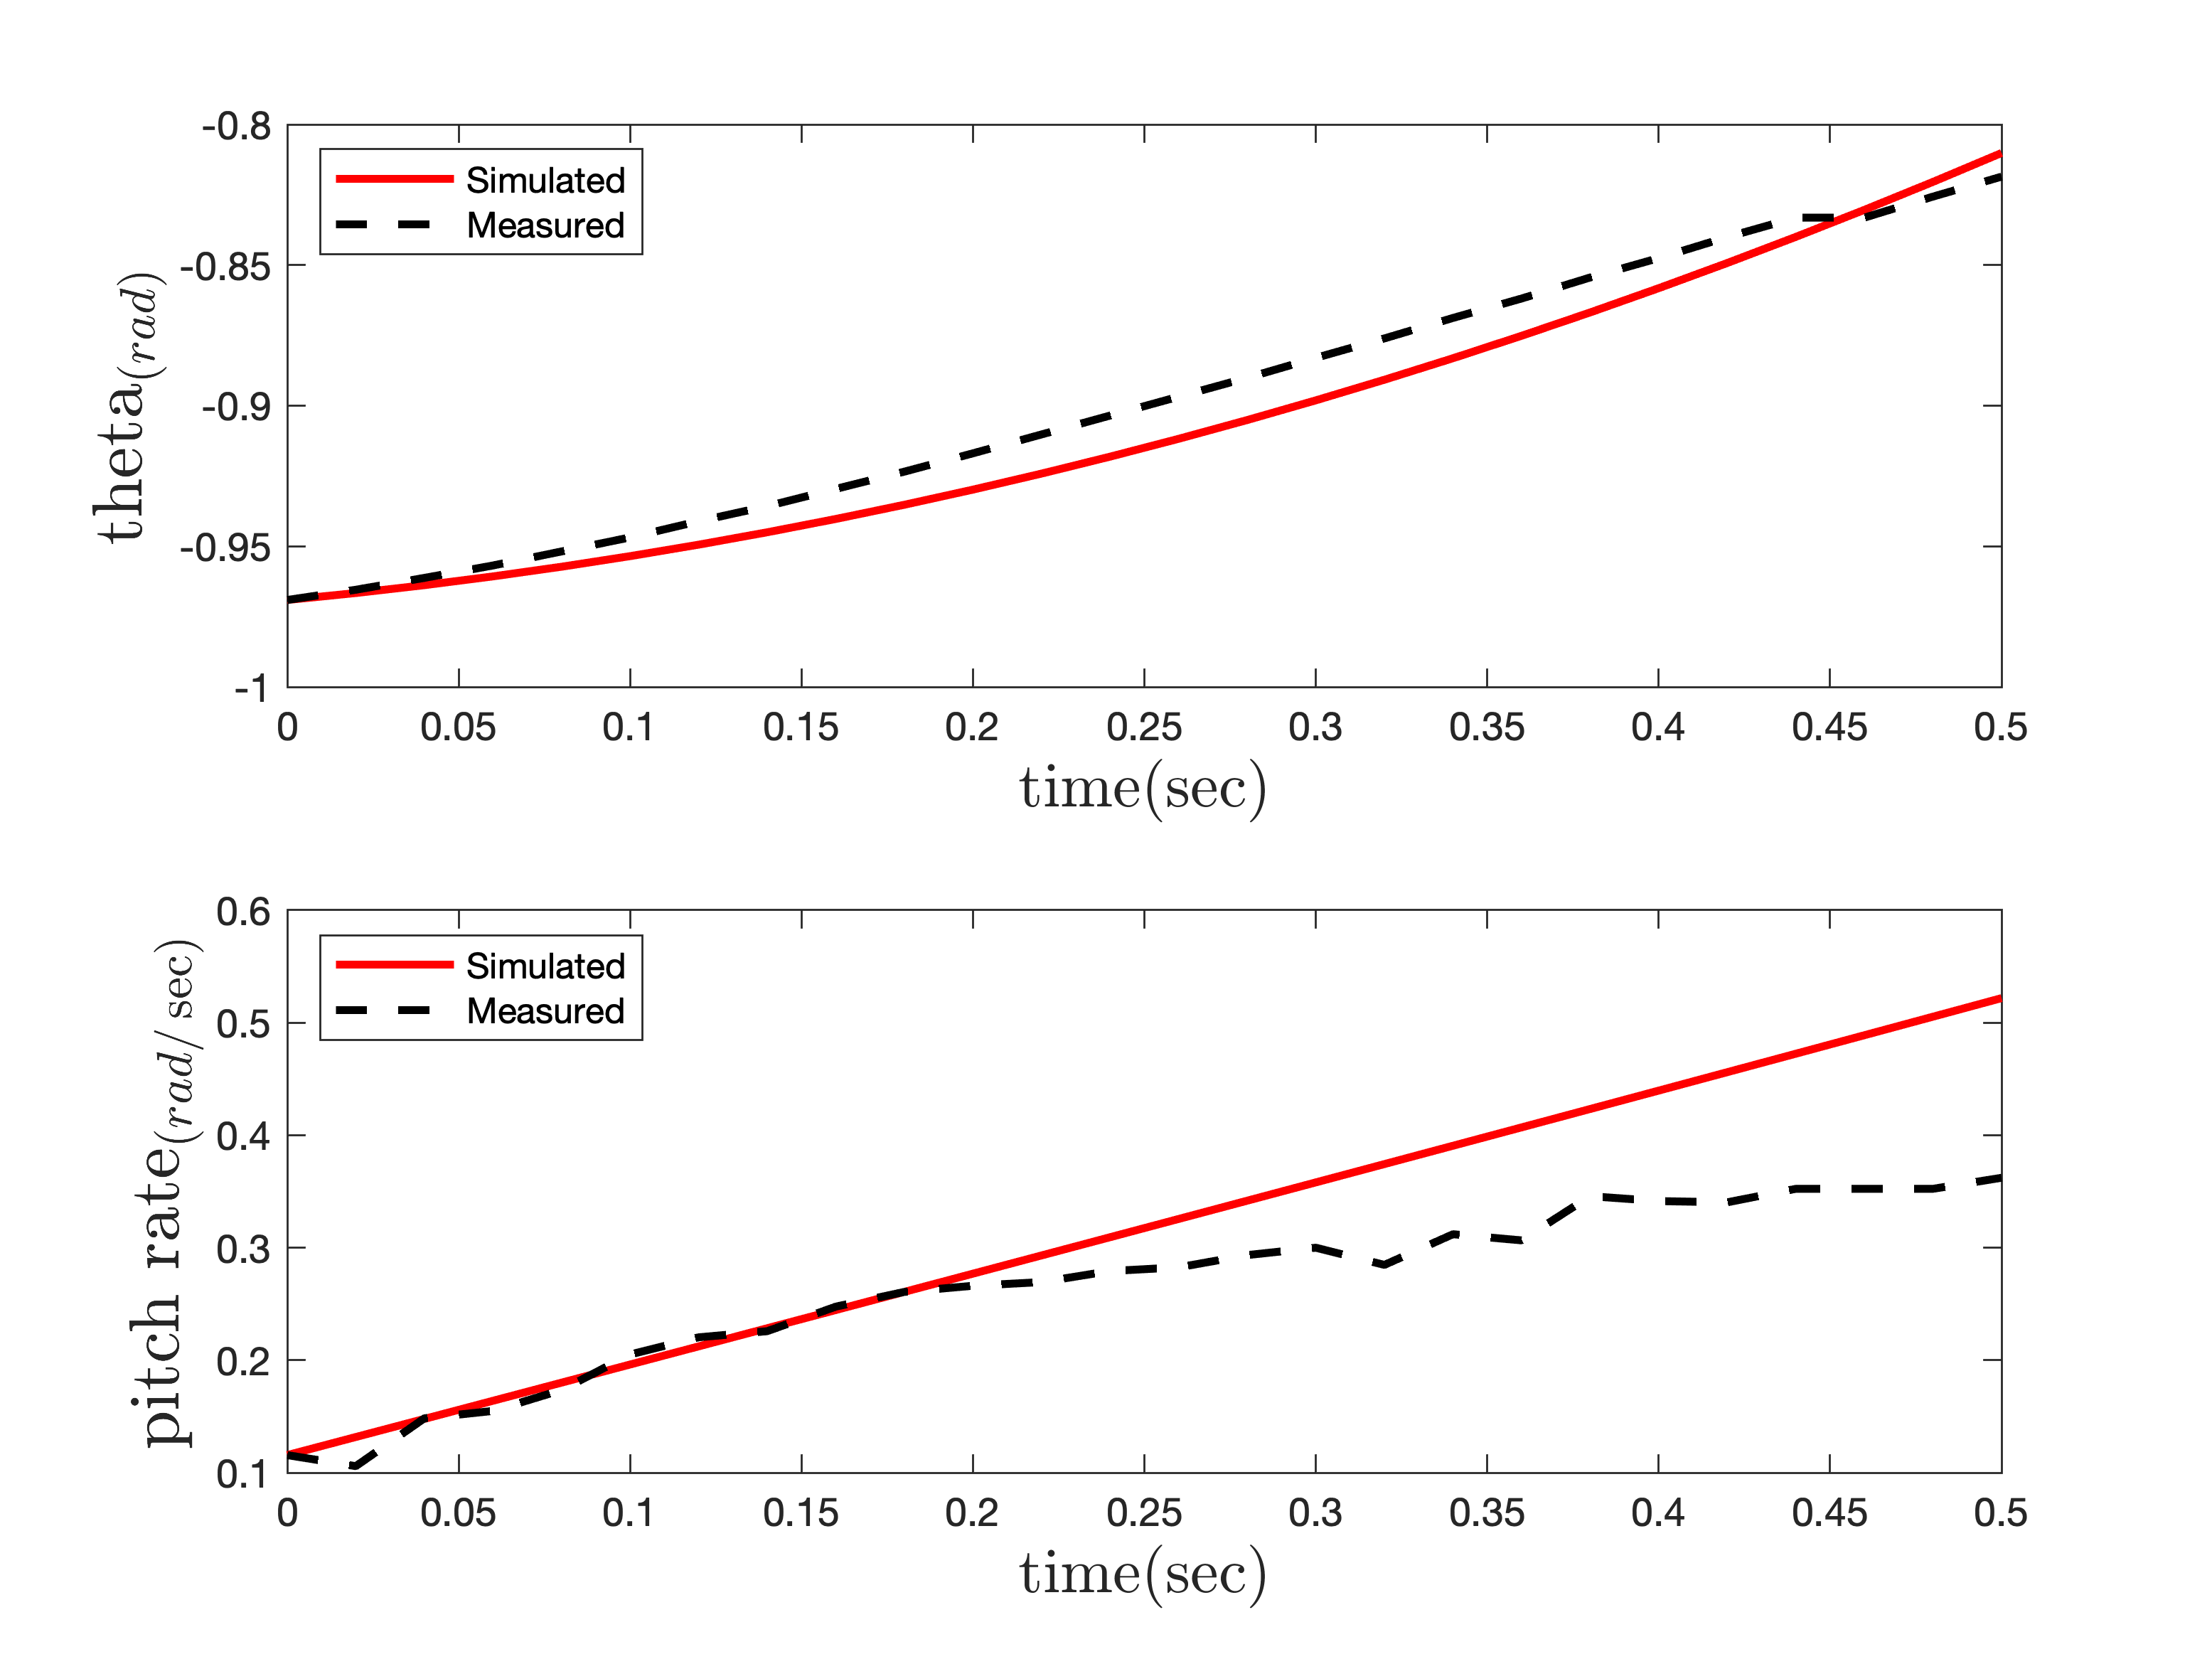
\includegraphics[width=12cm]{../Figures/RCP/pitch_parameter_estimation/RCP_pitch_S2.png}
	\centering
	\caption{مقايسه وضعیت استند در  آزمايش دوم و شبیه‌سازی، پس از تخمین پارامترهای کانال پپچ}
	\label{pitch_ps2}
\end{figure}
\begin{figure}[H]
	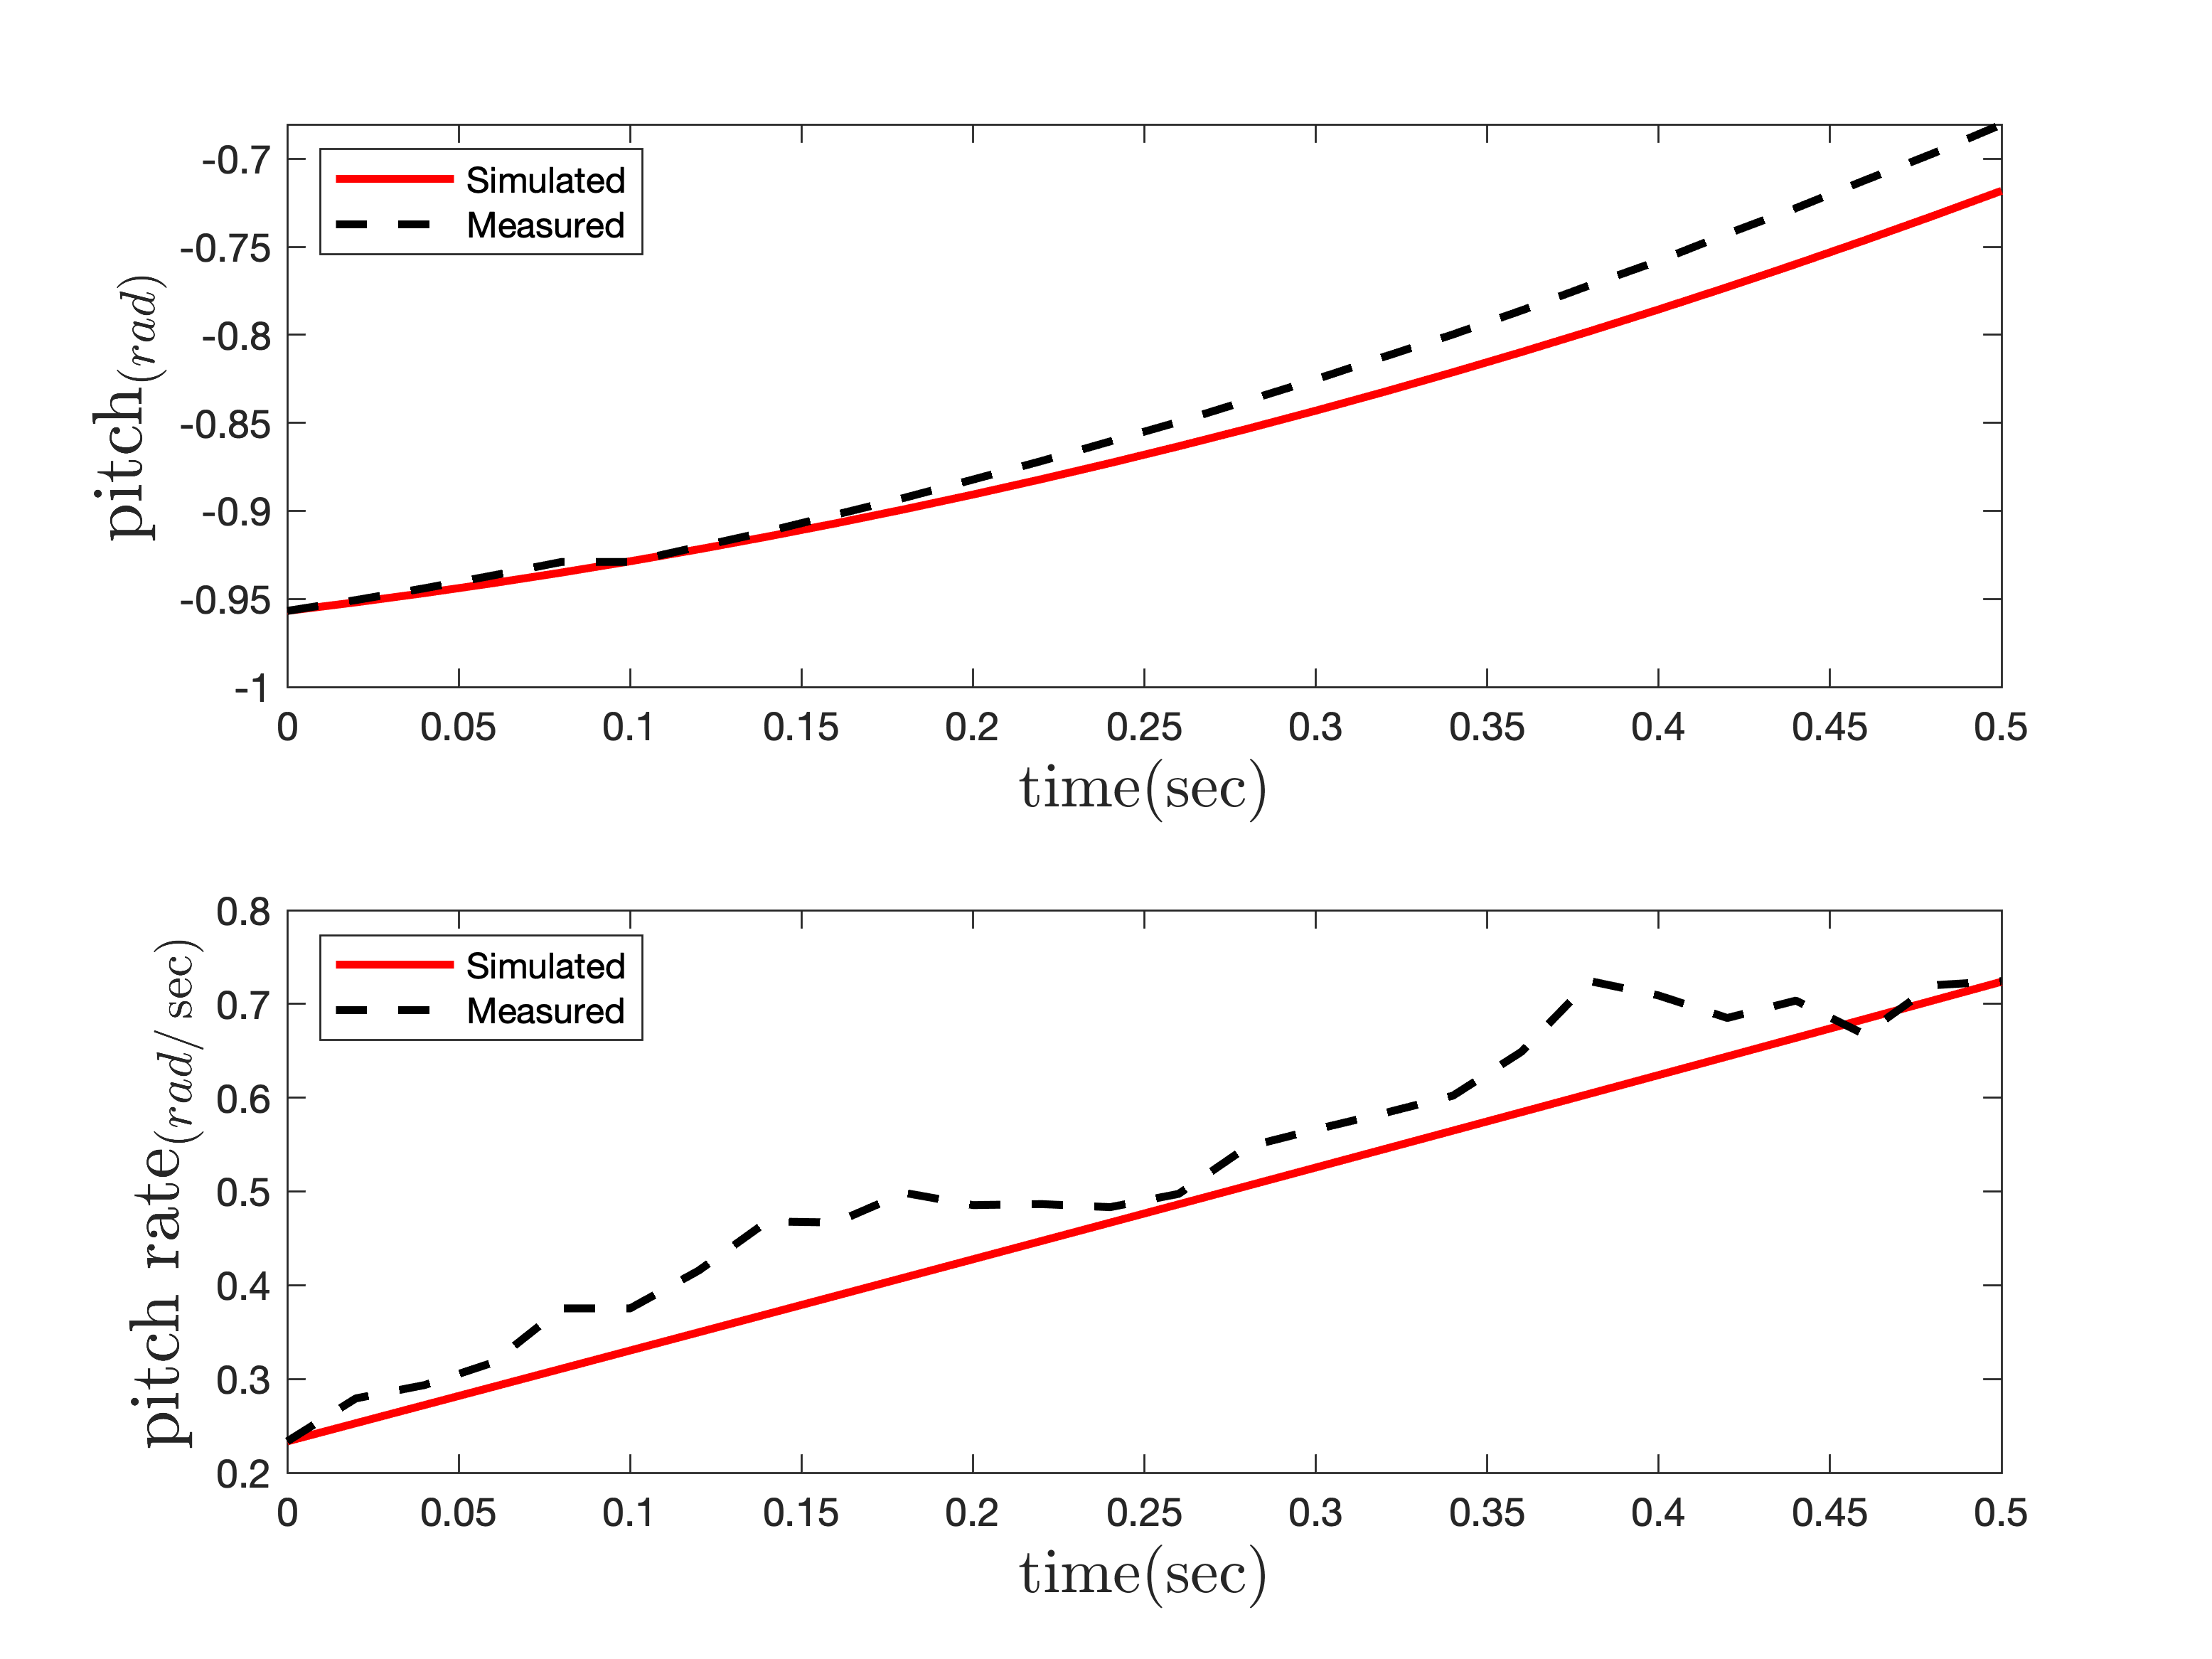
\includegraphics[width=12cm]{../Figures/RCP/pitch_parameter_estimation/RCP_pitch_S3.png}
	\centering
	\caption{مقايسه وضعیت استند در  آزمايش سوم و شبیه‌سازی، پس از تخمین پارامترهای کانال پپچ}
	\label{pitch_ps3}
\end{figure}

%\subsection{تخمین پارامتر کانال یاو}
برای اصلاح پارامترهای یاو چندین آزمایش انجام شد و با استفاده از داده‌های ثبت شده از وضعیت استند در کانال پیچ  و جعبه‌ابزار
\lr{Parameter Estimator}
پارامترها اصلاح شدند.
برای آزمایش یاو همه‌ی موتورها با دور مختلف شروع به حرکت کردند و از خروجی‌ سنسور داده برداری شد. سپس، مدل و پارامترهای داده‌های ثبت شده‌ی سنسور (وضعیت استند در کانال یاو) به جعبه‌ابزار
\lr{Parameter Estimator}
داده شد. نتایج آزمایش‌های کانال یاو بعد از اصلاح پارامترها در شکل
\ref{yaw_ps1} و \ref{yaw_ps2}
آورده شده است.

\begin{figure}[H]
	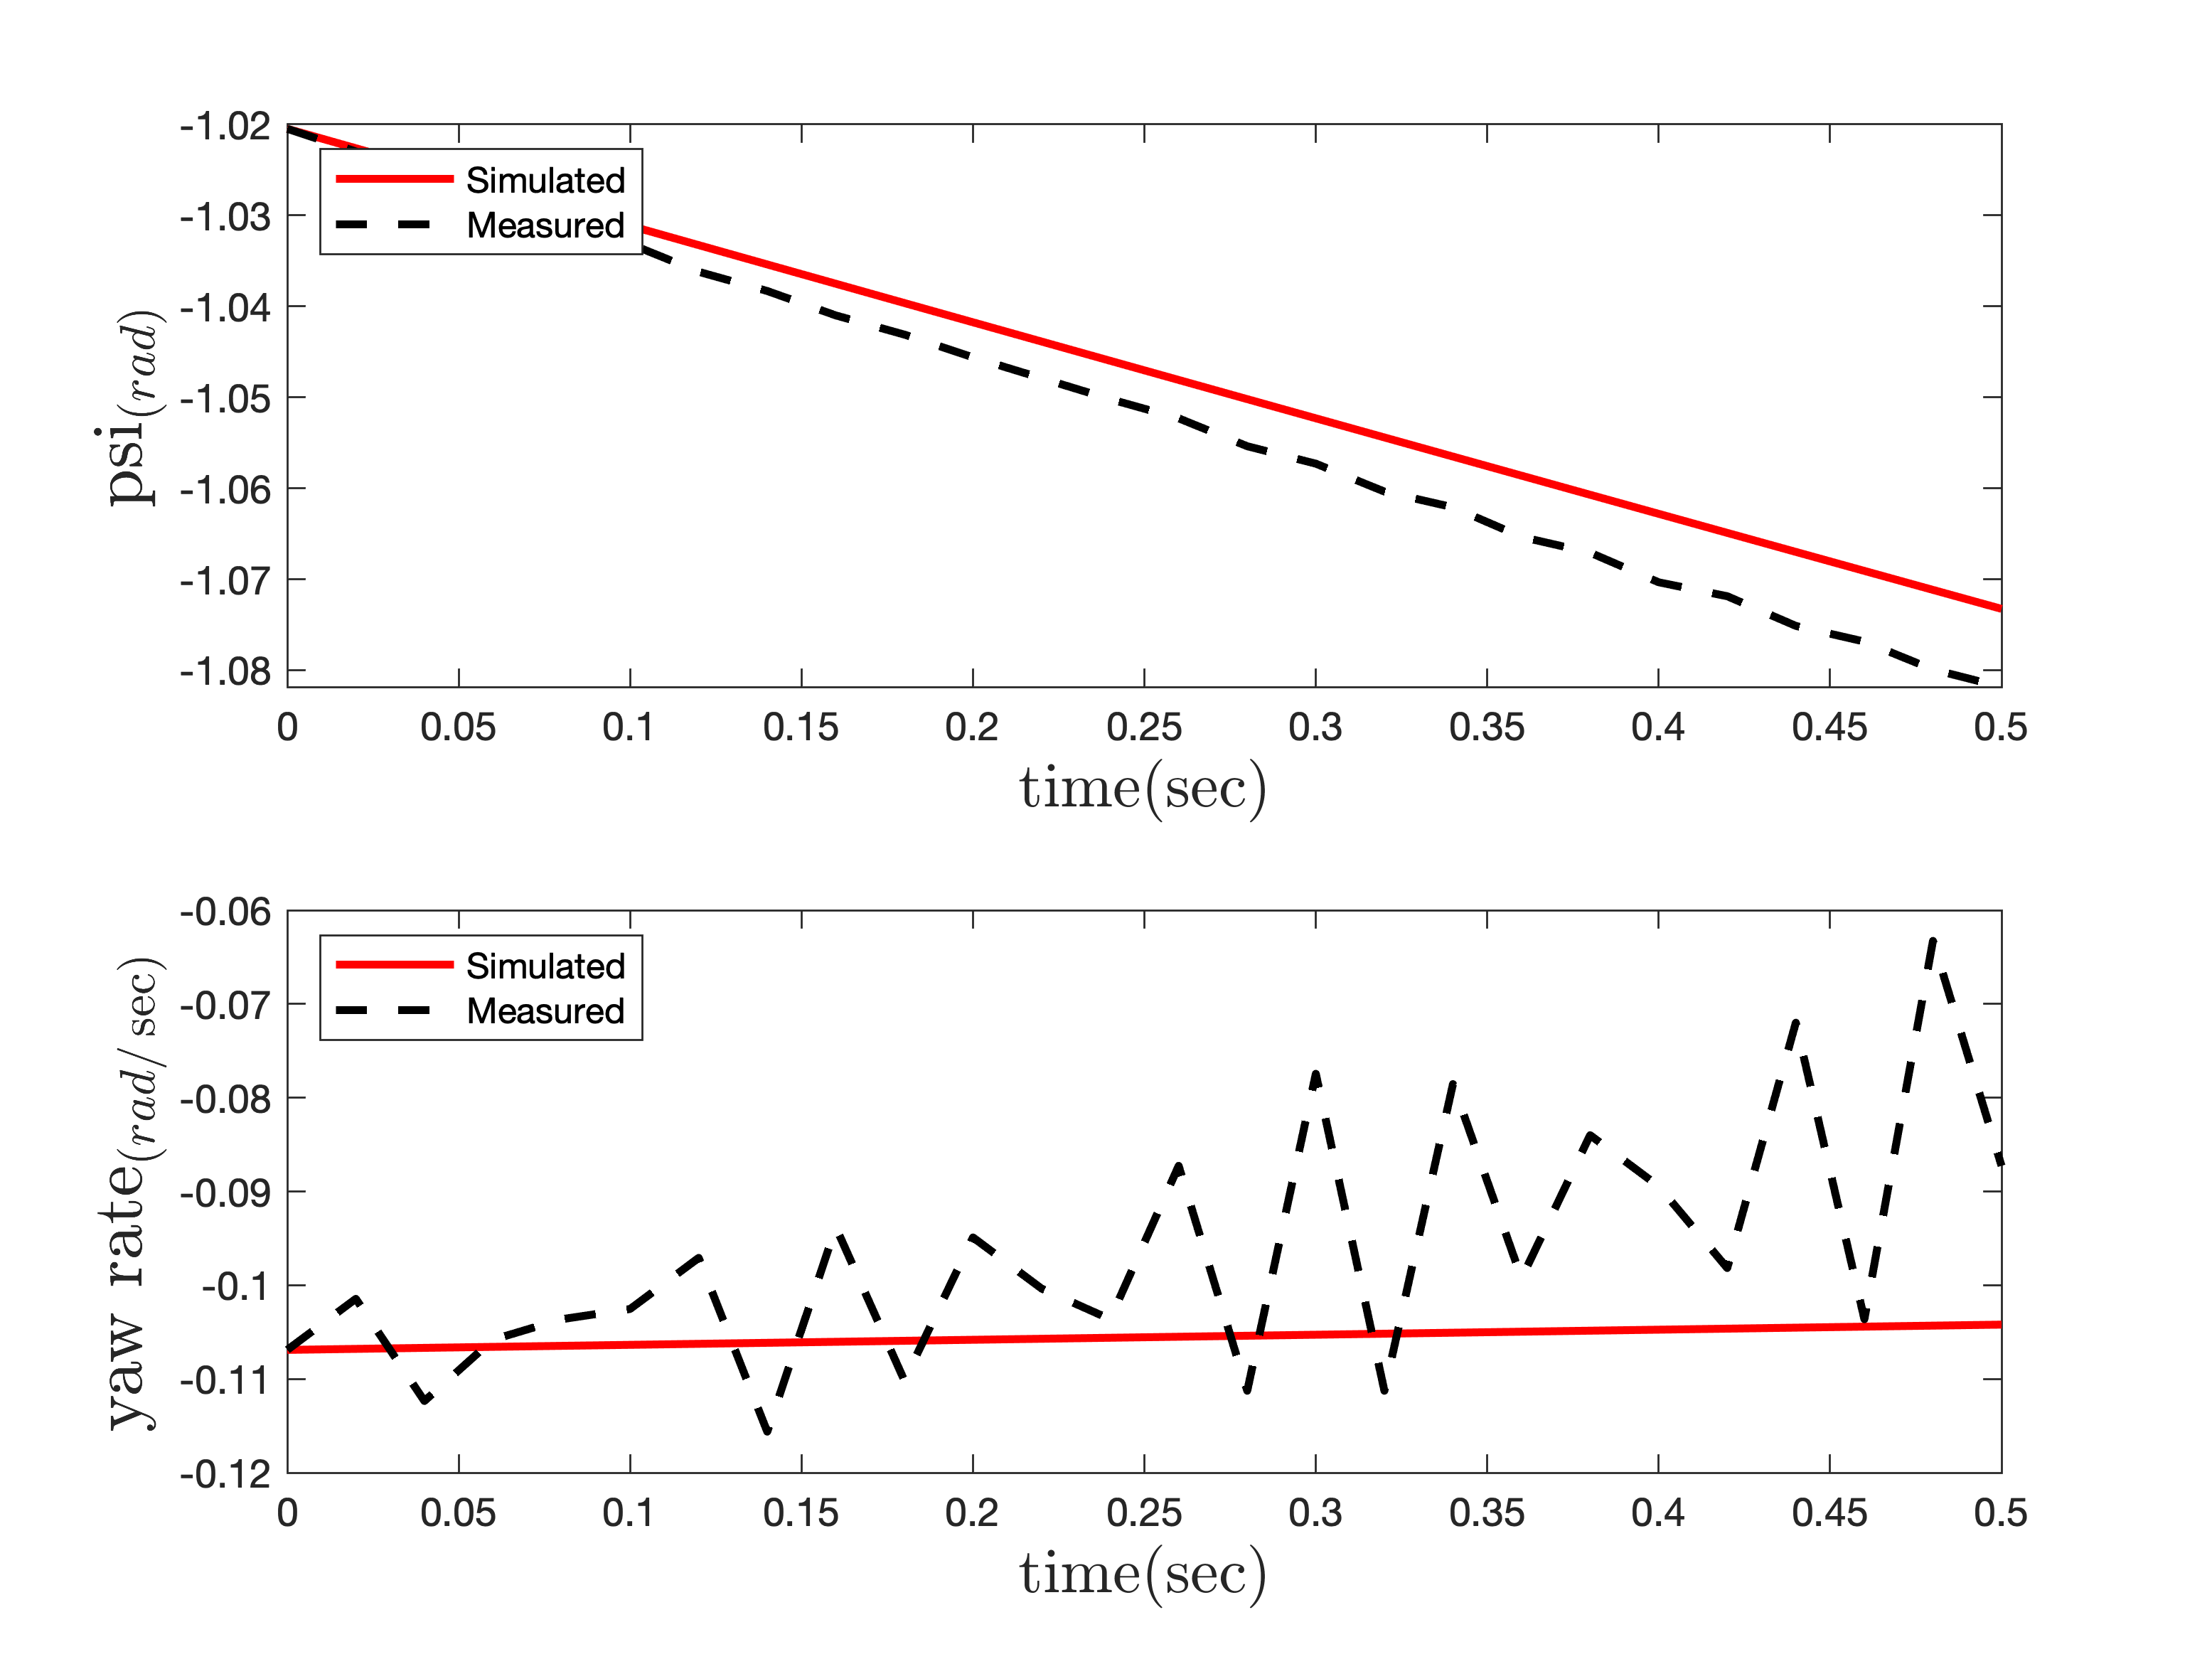
\includegraphics[width=12cm]{../Figures/RCP/yaw_parameter_estimation/RCP_yaw_S1.png}
	\centering
	\caption{مقايسه وضعیت استند در  آزمايش اول و شبیه‌سازی، پس از تخمین پارامترهای کانال یاو}
	\label{yaw_ps1}
\end{figure}

\begin{figure}[H]
	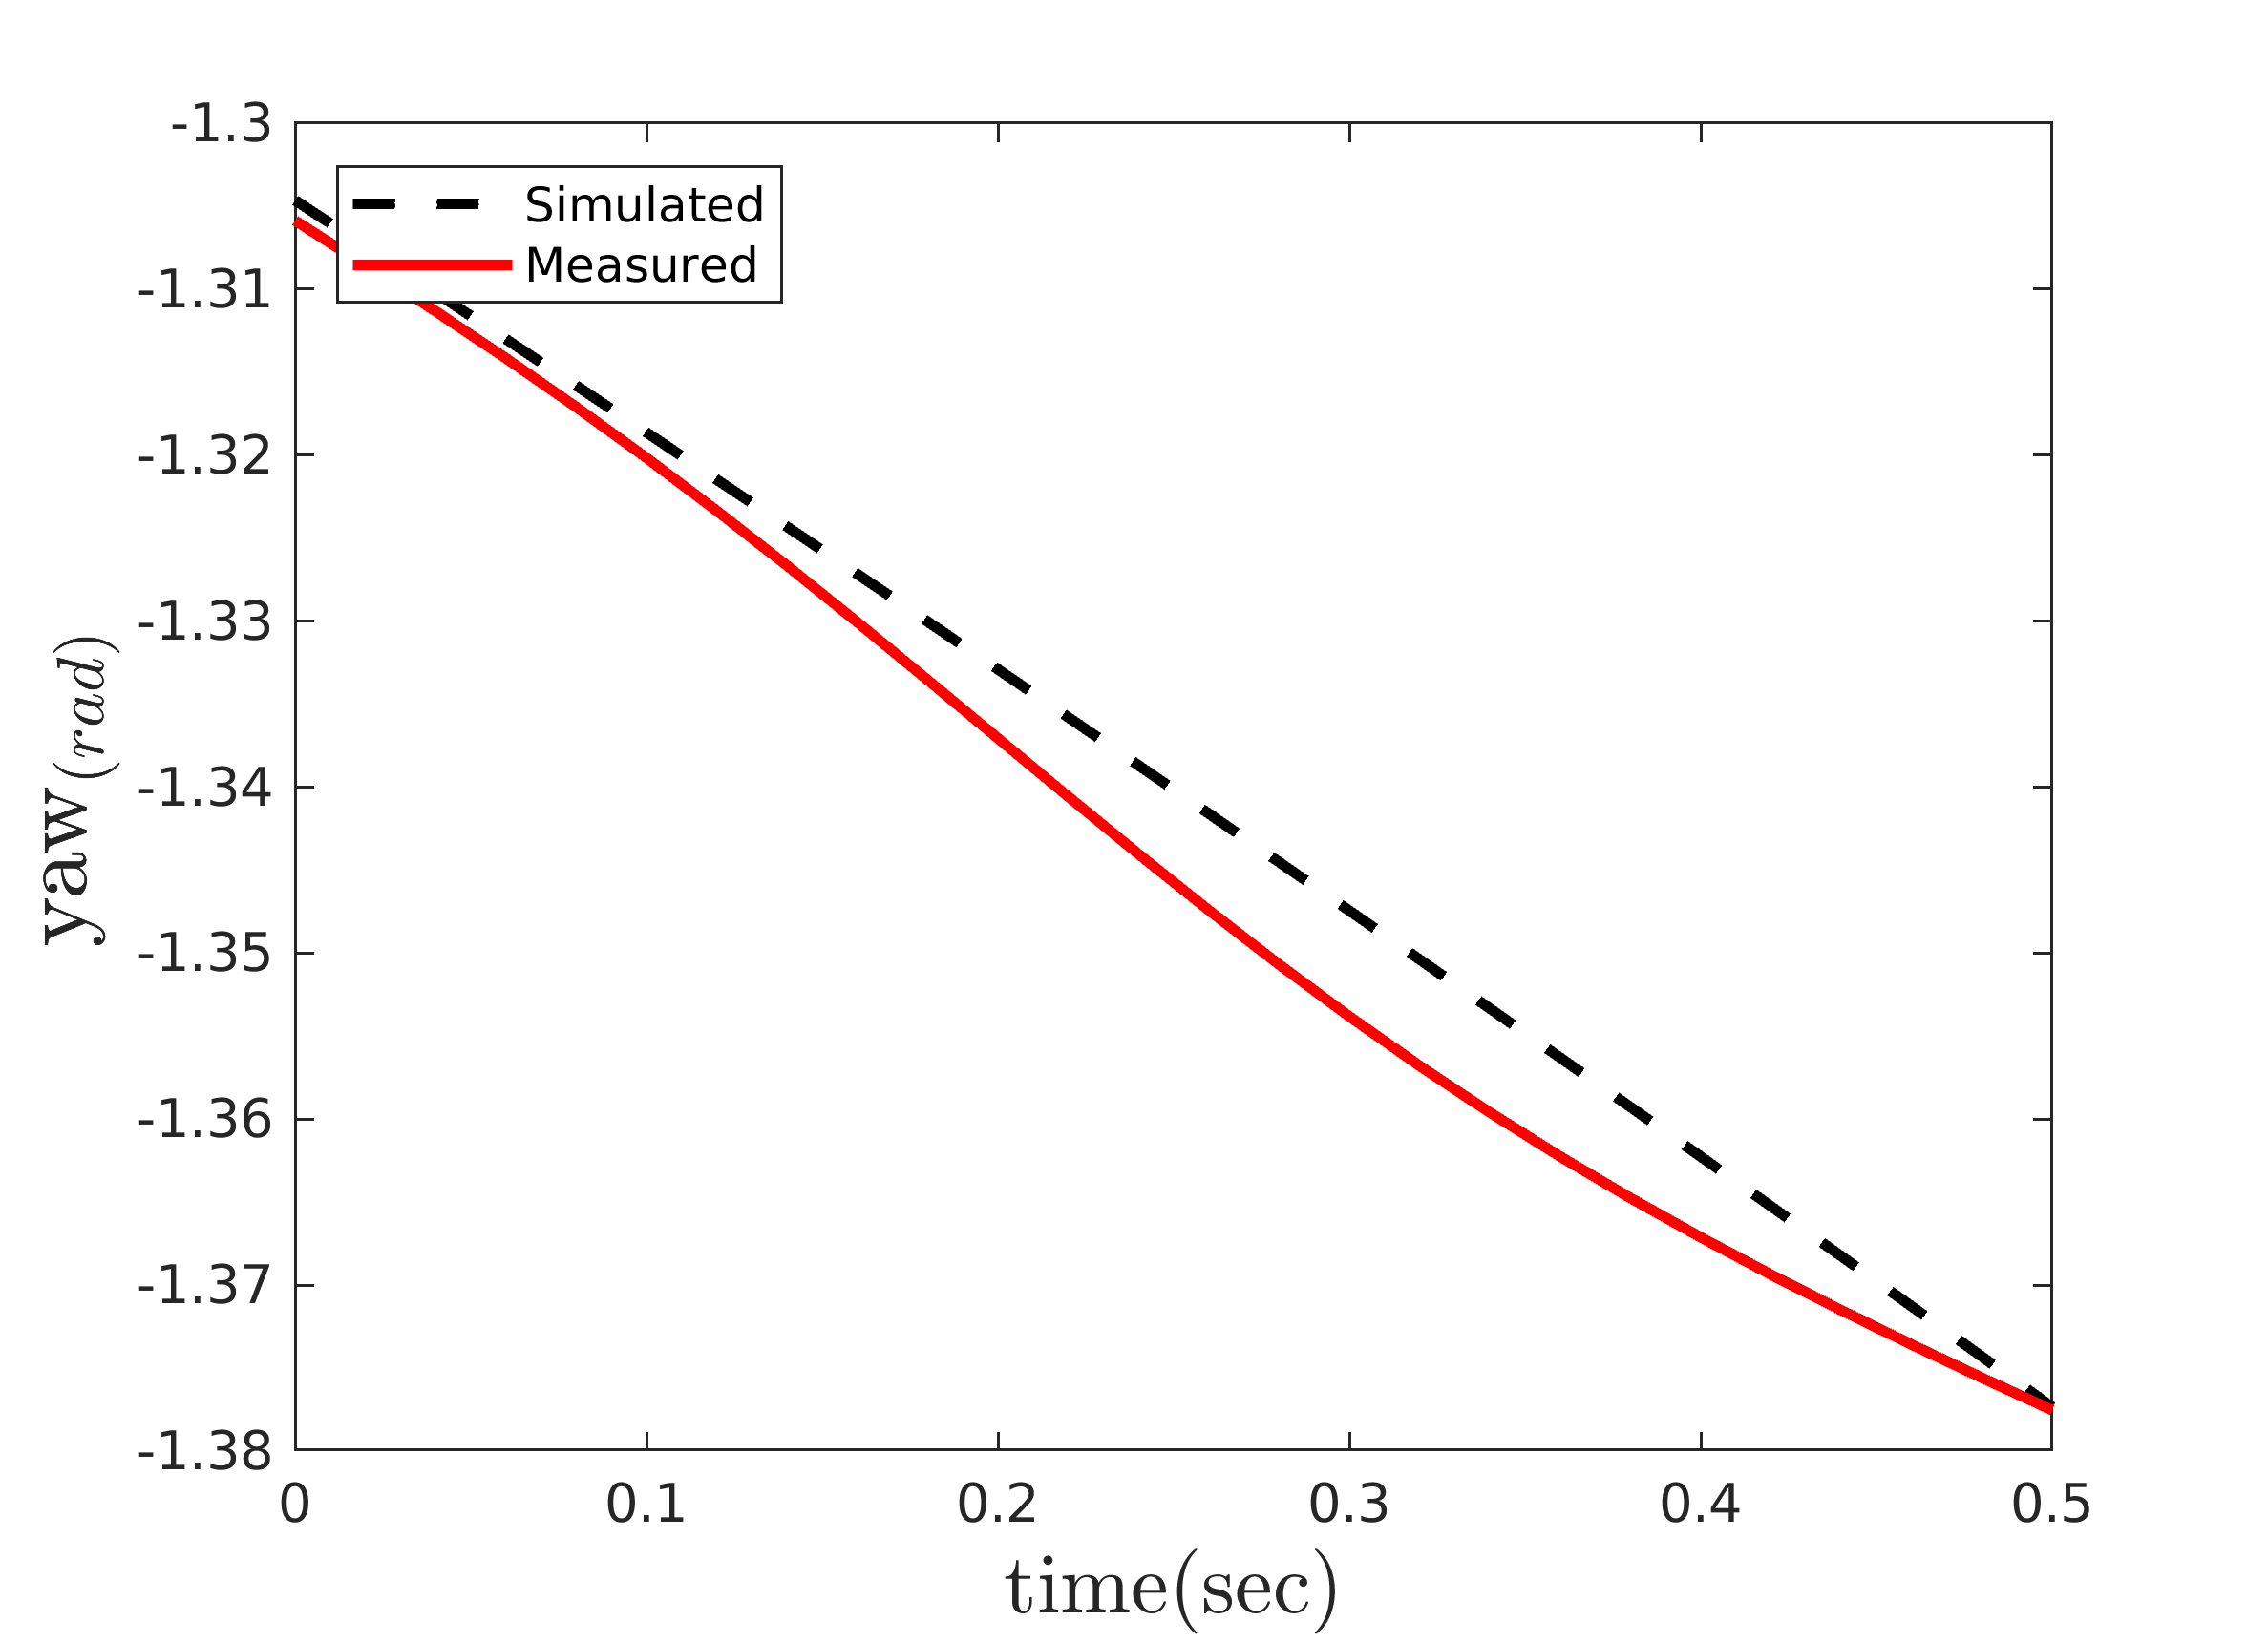
\includegraphics[width=12cm]{../Figures/RCP/yaw_parameter_estimation/RCP_yaw_S2.png}
	\centering
	\caption{مقايسه وضعیت استند در  آزمايش دوم و شبیه‌سازی، پس از تخمین پارامترهای کانال یاو}
	\label{yaw_ps2}
\end{figure}
%\subsection{تخمین پارامتر کانال‌های رول-پیچ}
برای اصلاح پارامترها رول-پیچ چندین آزمایش انجام شد و با استفاده از داده‌های ثبت شده از وضعیت استند در کانال رول-پپچ و جعبه‌ابزار
\lr{Parameter Estimator}
پارامترهای کانال رول-پیچ اصلاح شدند.
برای آزمایش تمامی موتورها با دور مختلف شروع به حرکت کردند و از خروجی سنسور داده برداری شد. سپس، مدل و  داده‌های ثبت شده سنسور (وضعیت استند در کانال رول-پیج)  به جعبه‌ابزار
\lr{Parameter Estimator}
داده شد. وضعیت کانال رول-پیچ استند در شبیه‌سازی و واقعیت بعد از اصلاح پارامترهای کانال‌ رول-پیچ بعد در شکل‌های
(\ref{roll_pitch_ps1}, \ref{roll_pitch_ps2}, \ref{roll_pitch_ps3}, \ref{roll_pitch_ps4}, \ref{roll_pitch_ps5}, \ref{roll_pitch_ps6}, \ref{roll_pitch_ps7})
آورده شده است.

\begin{figure}[H]
	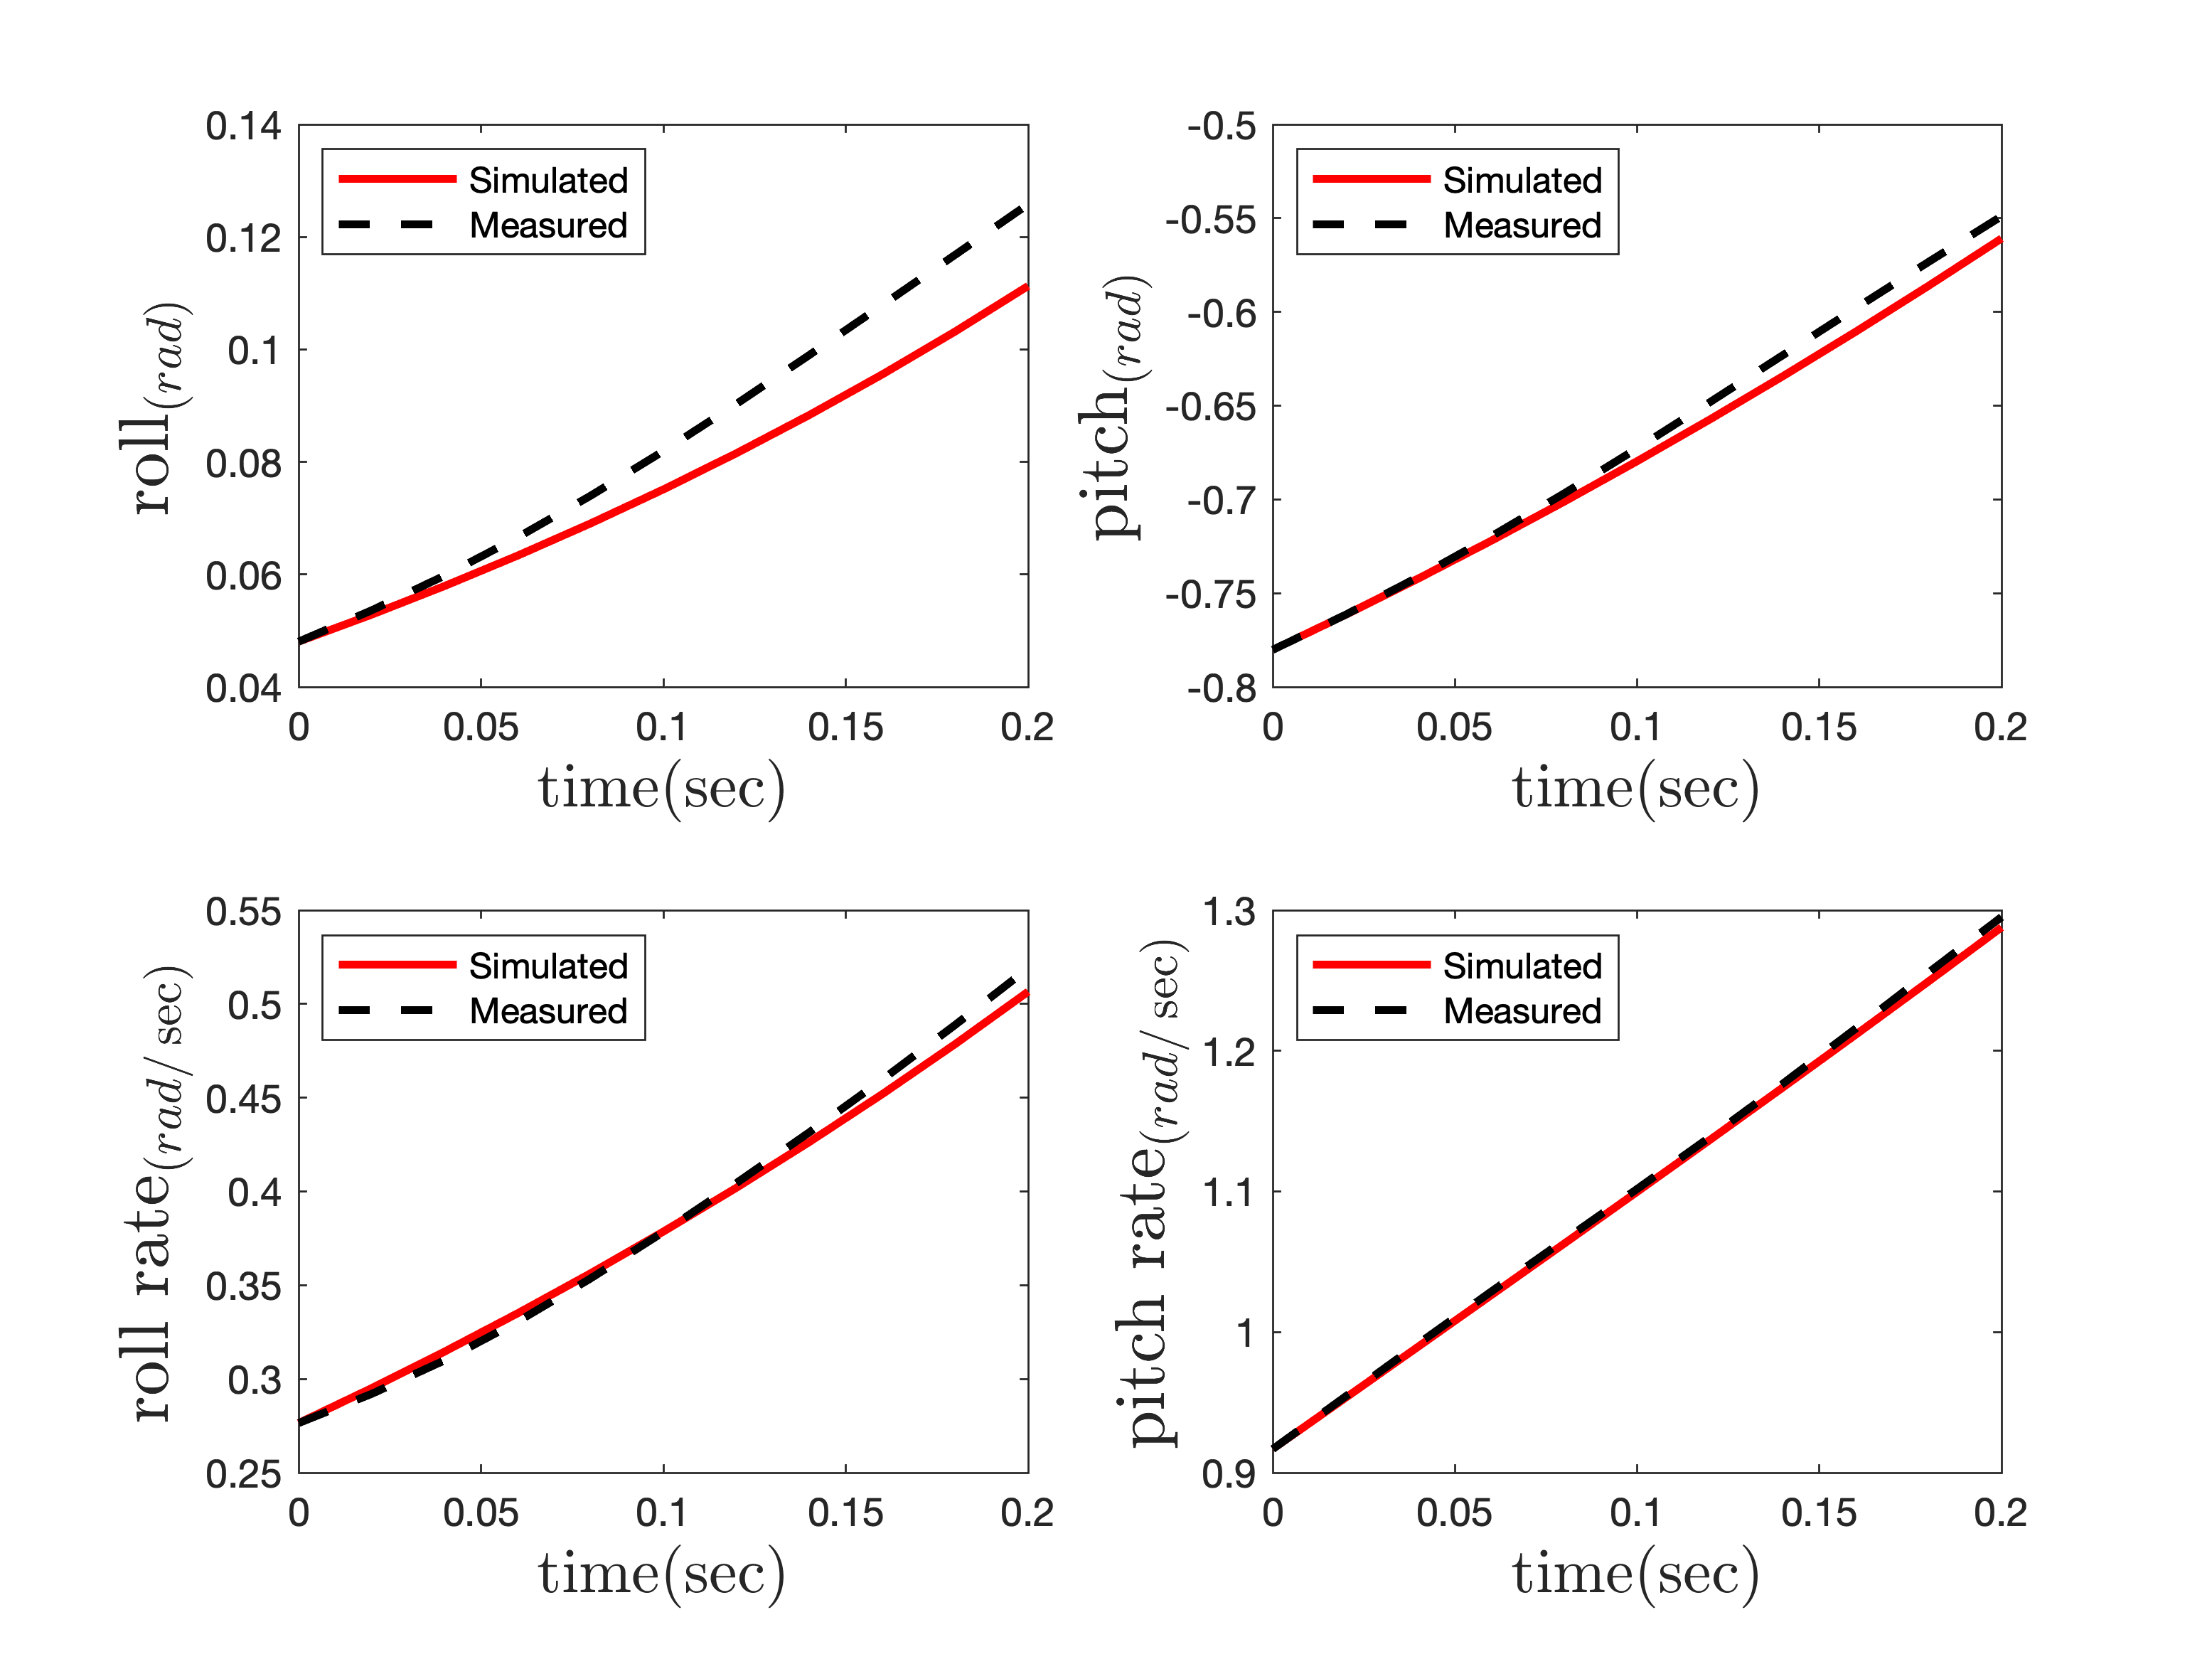
\includegraphics[width=12cm]{../../Figures/RCP/roll_pitch_parameter_estimation/RCP_roll_pitch_S1.png}
	\centering
	\caption{مقايسه وضعیت استند در  آزمايش اول و شبیه‌سازی، پس از تخمین پارامترهای کانال رول-پیچ}
	\label{roll_pitch_ps1}
\end{figure}
\begin{figure}[H]
	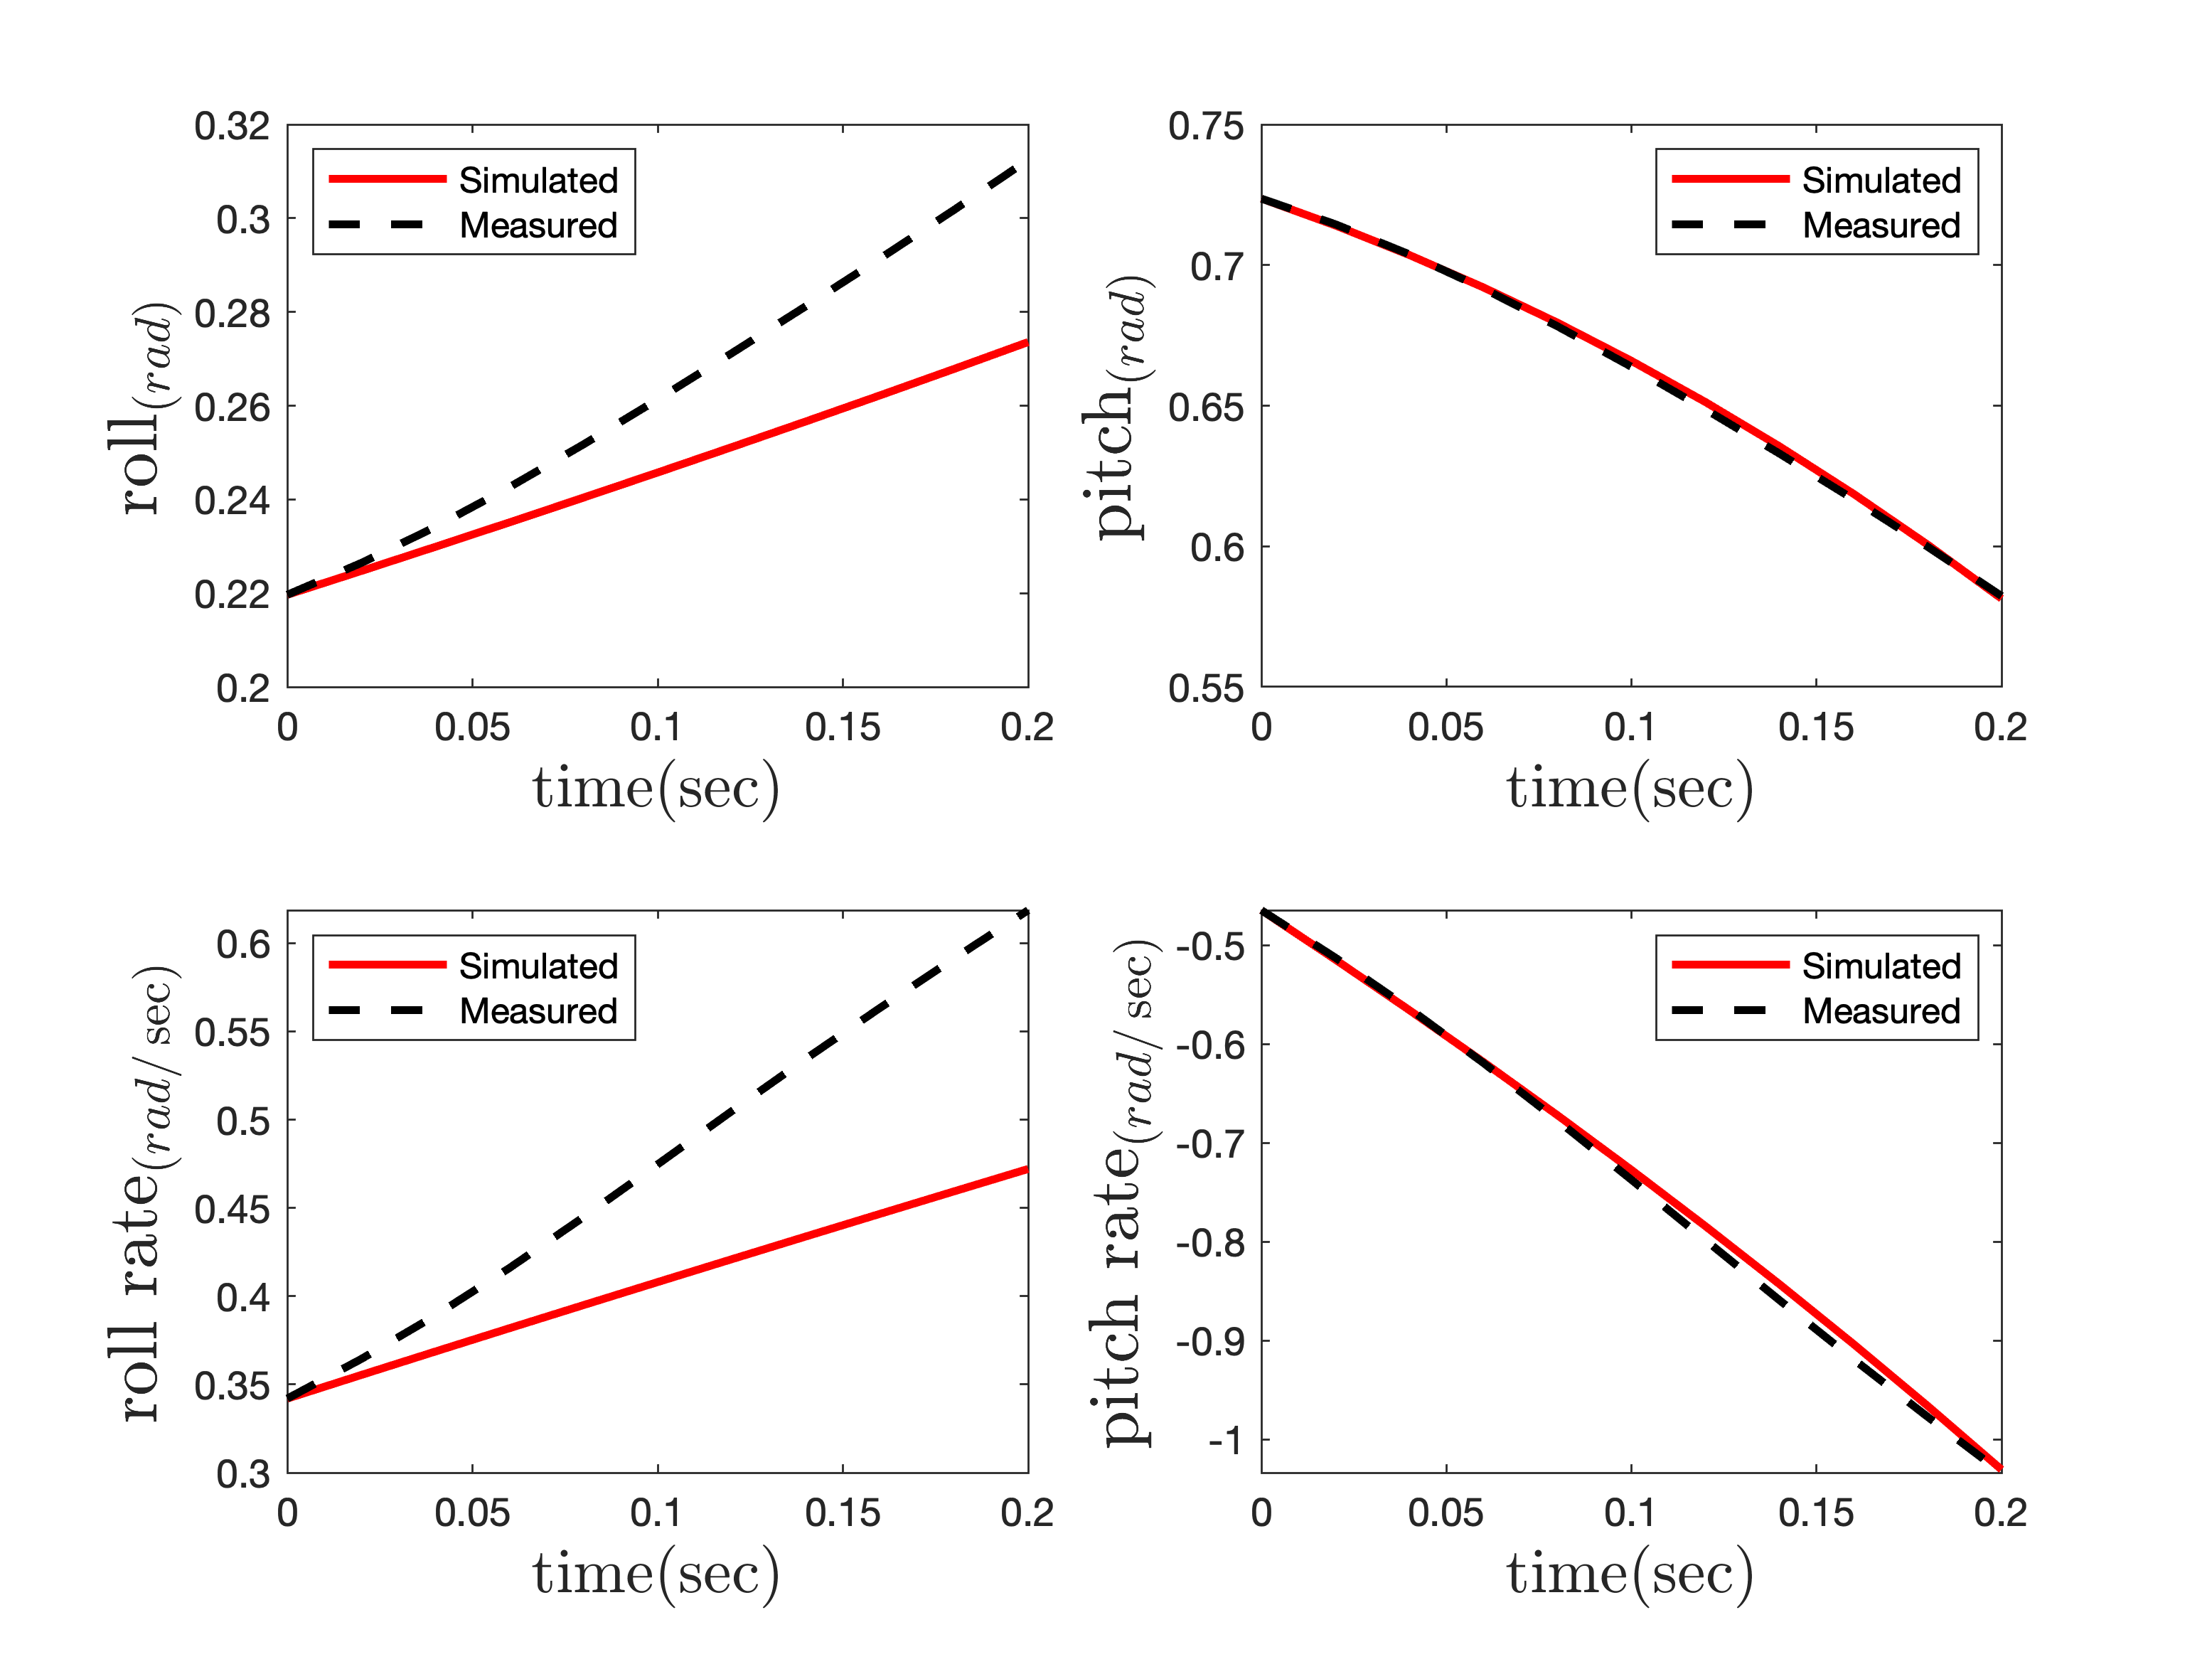
\includegraphics[width=12cm]{../../Figures/RCP/roll_pitch_parameter_estimation/RCP_roll_pitch_S2.png}
	\centering
	\caption{مقايسه وضعیت استند در  آزمايش دوم و شبیه‌سازی، پس از تخمین پارامترهای کانال رول-پیچ}
	\label{roll_pitch_ps2}
\end{figure}
\begin{figure}[H]
	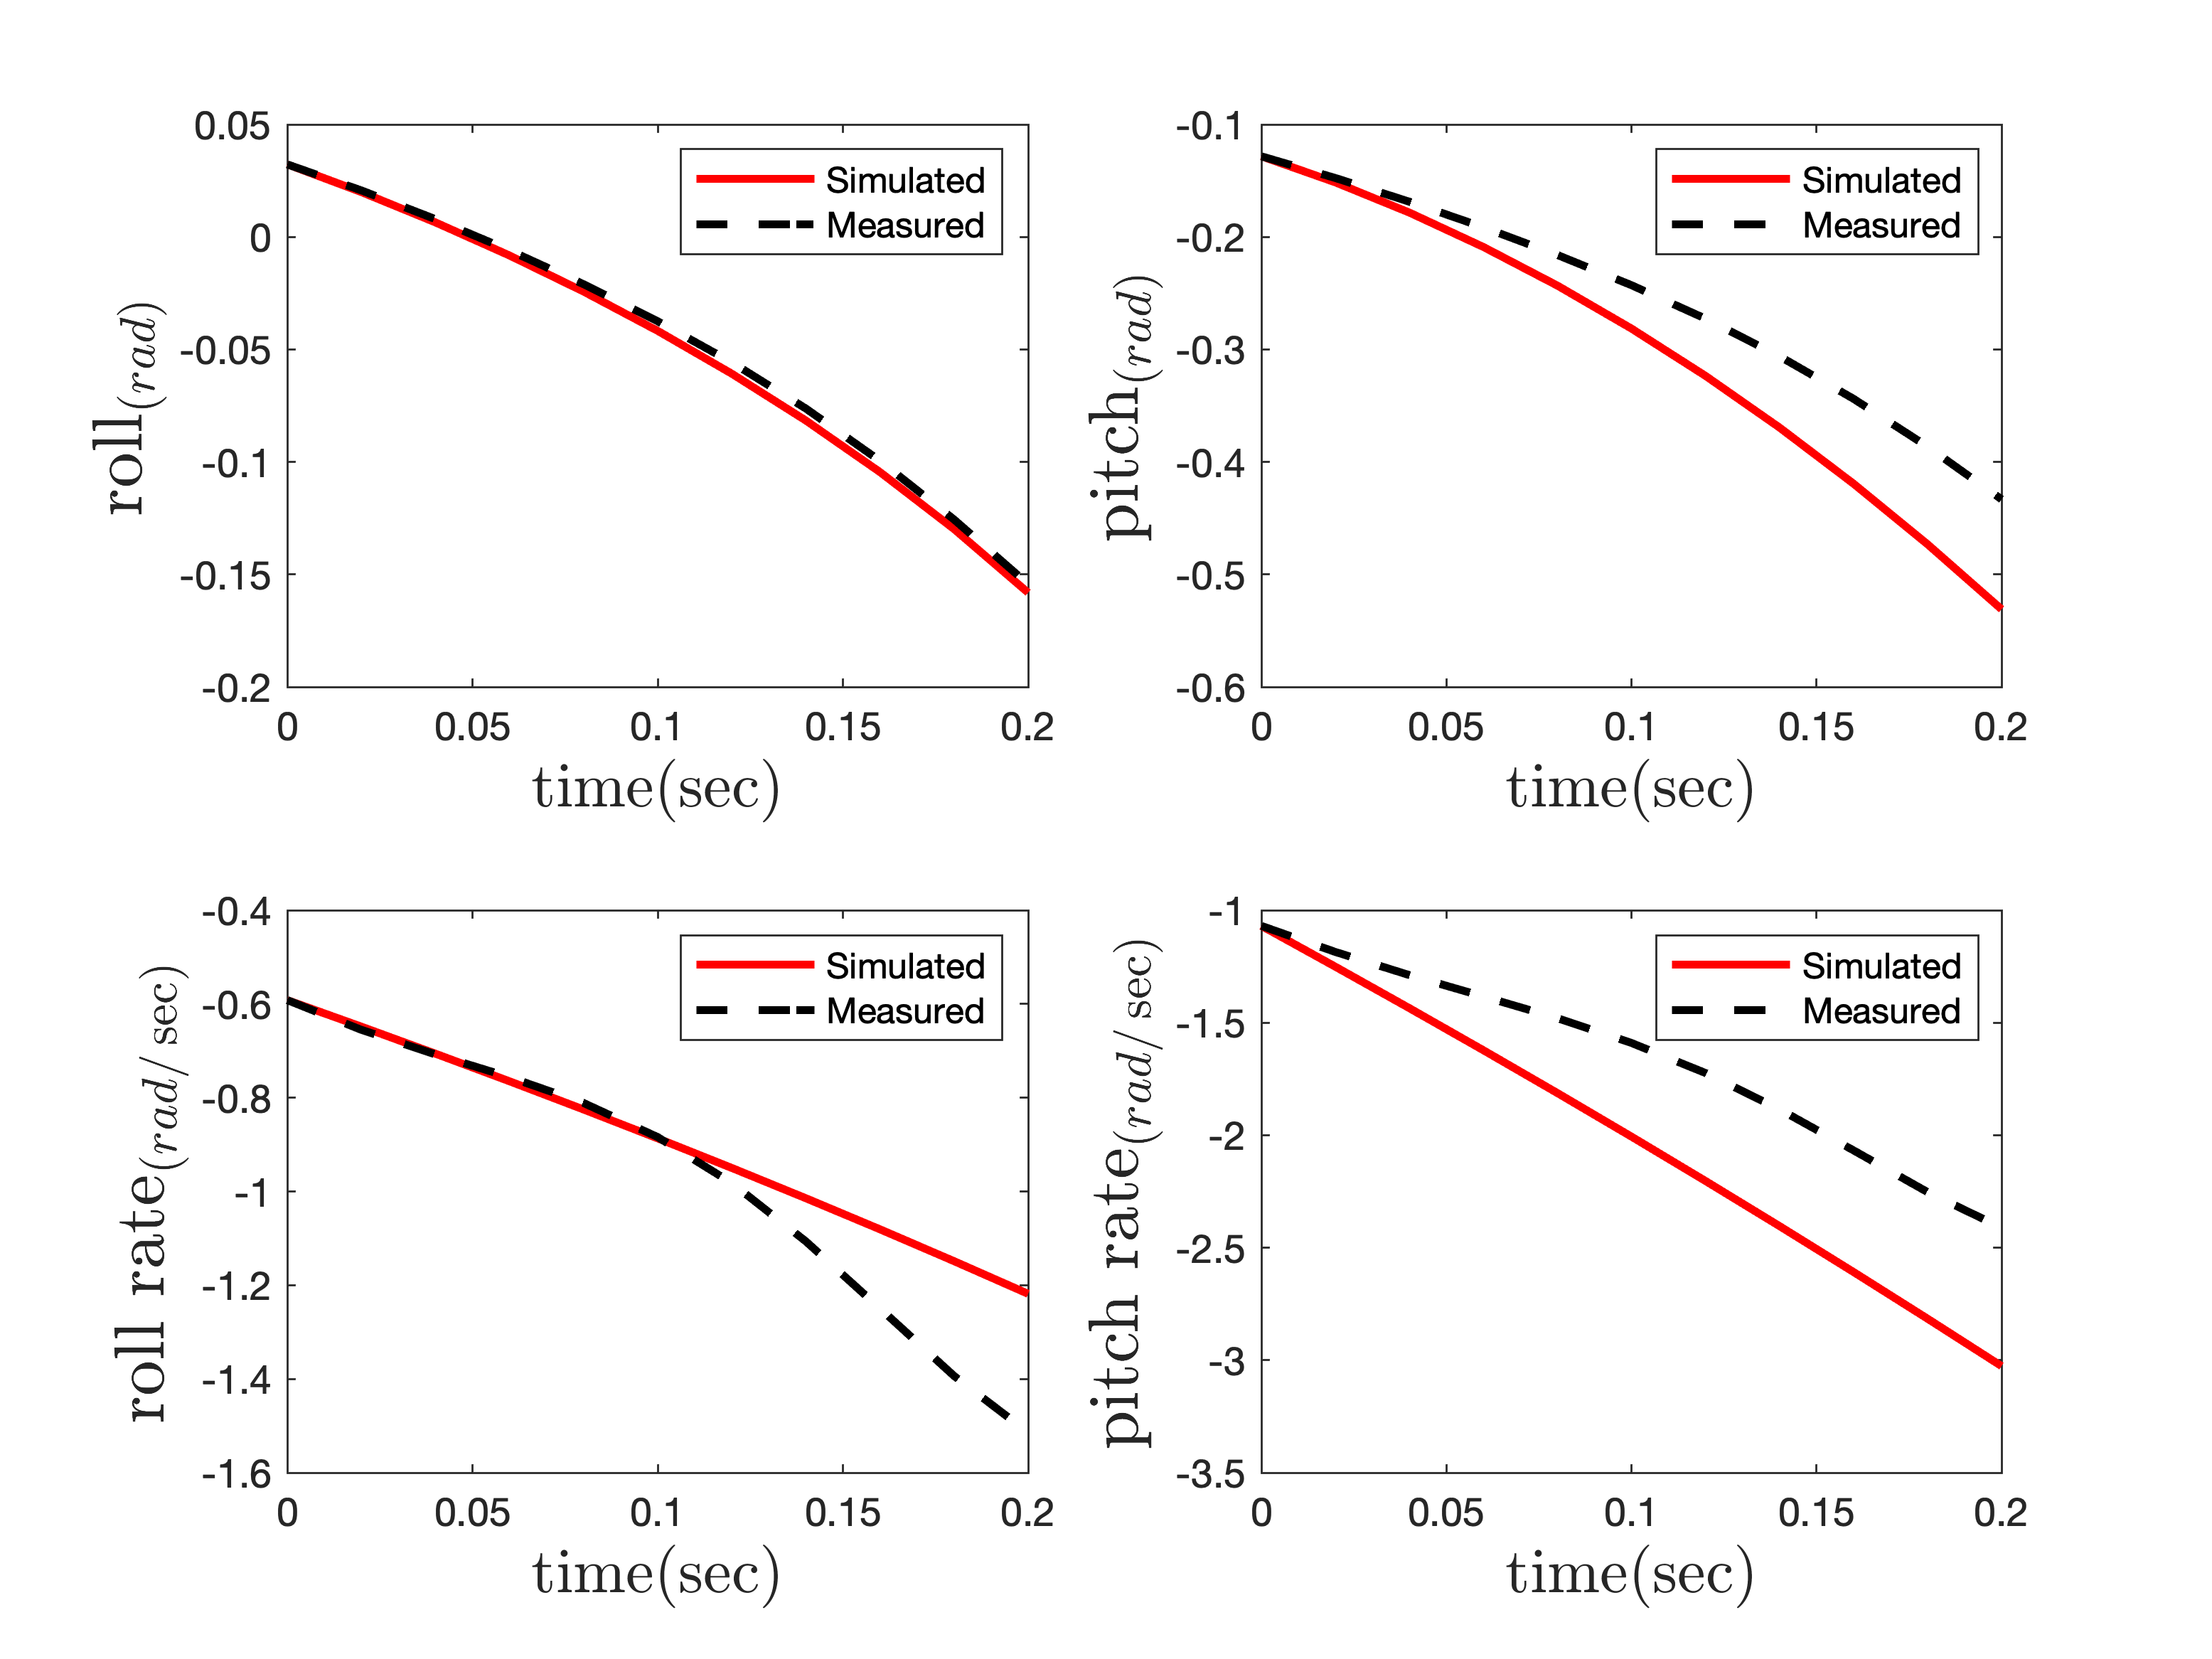
\includegraphics[width=12cm]{../../Figures/RCP/roll_pitch_parameter_estimation/RCP_roll_pitch_S3.png}
	\centering
	\caption{مقايسه وضعیت استند در  آزمايش سوم و شبیه‌سازی، پس از تخمین پارامترهای کانال رول-پیچ}
	\label{roll_pitch_ps3}
\end{figure}
\begin{figure}[H]
	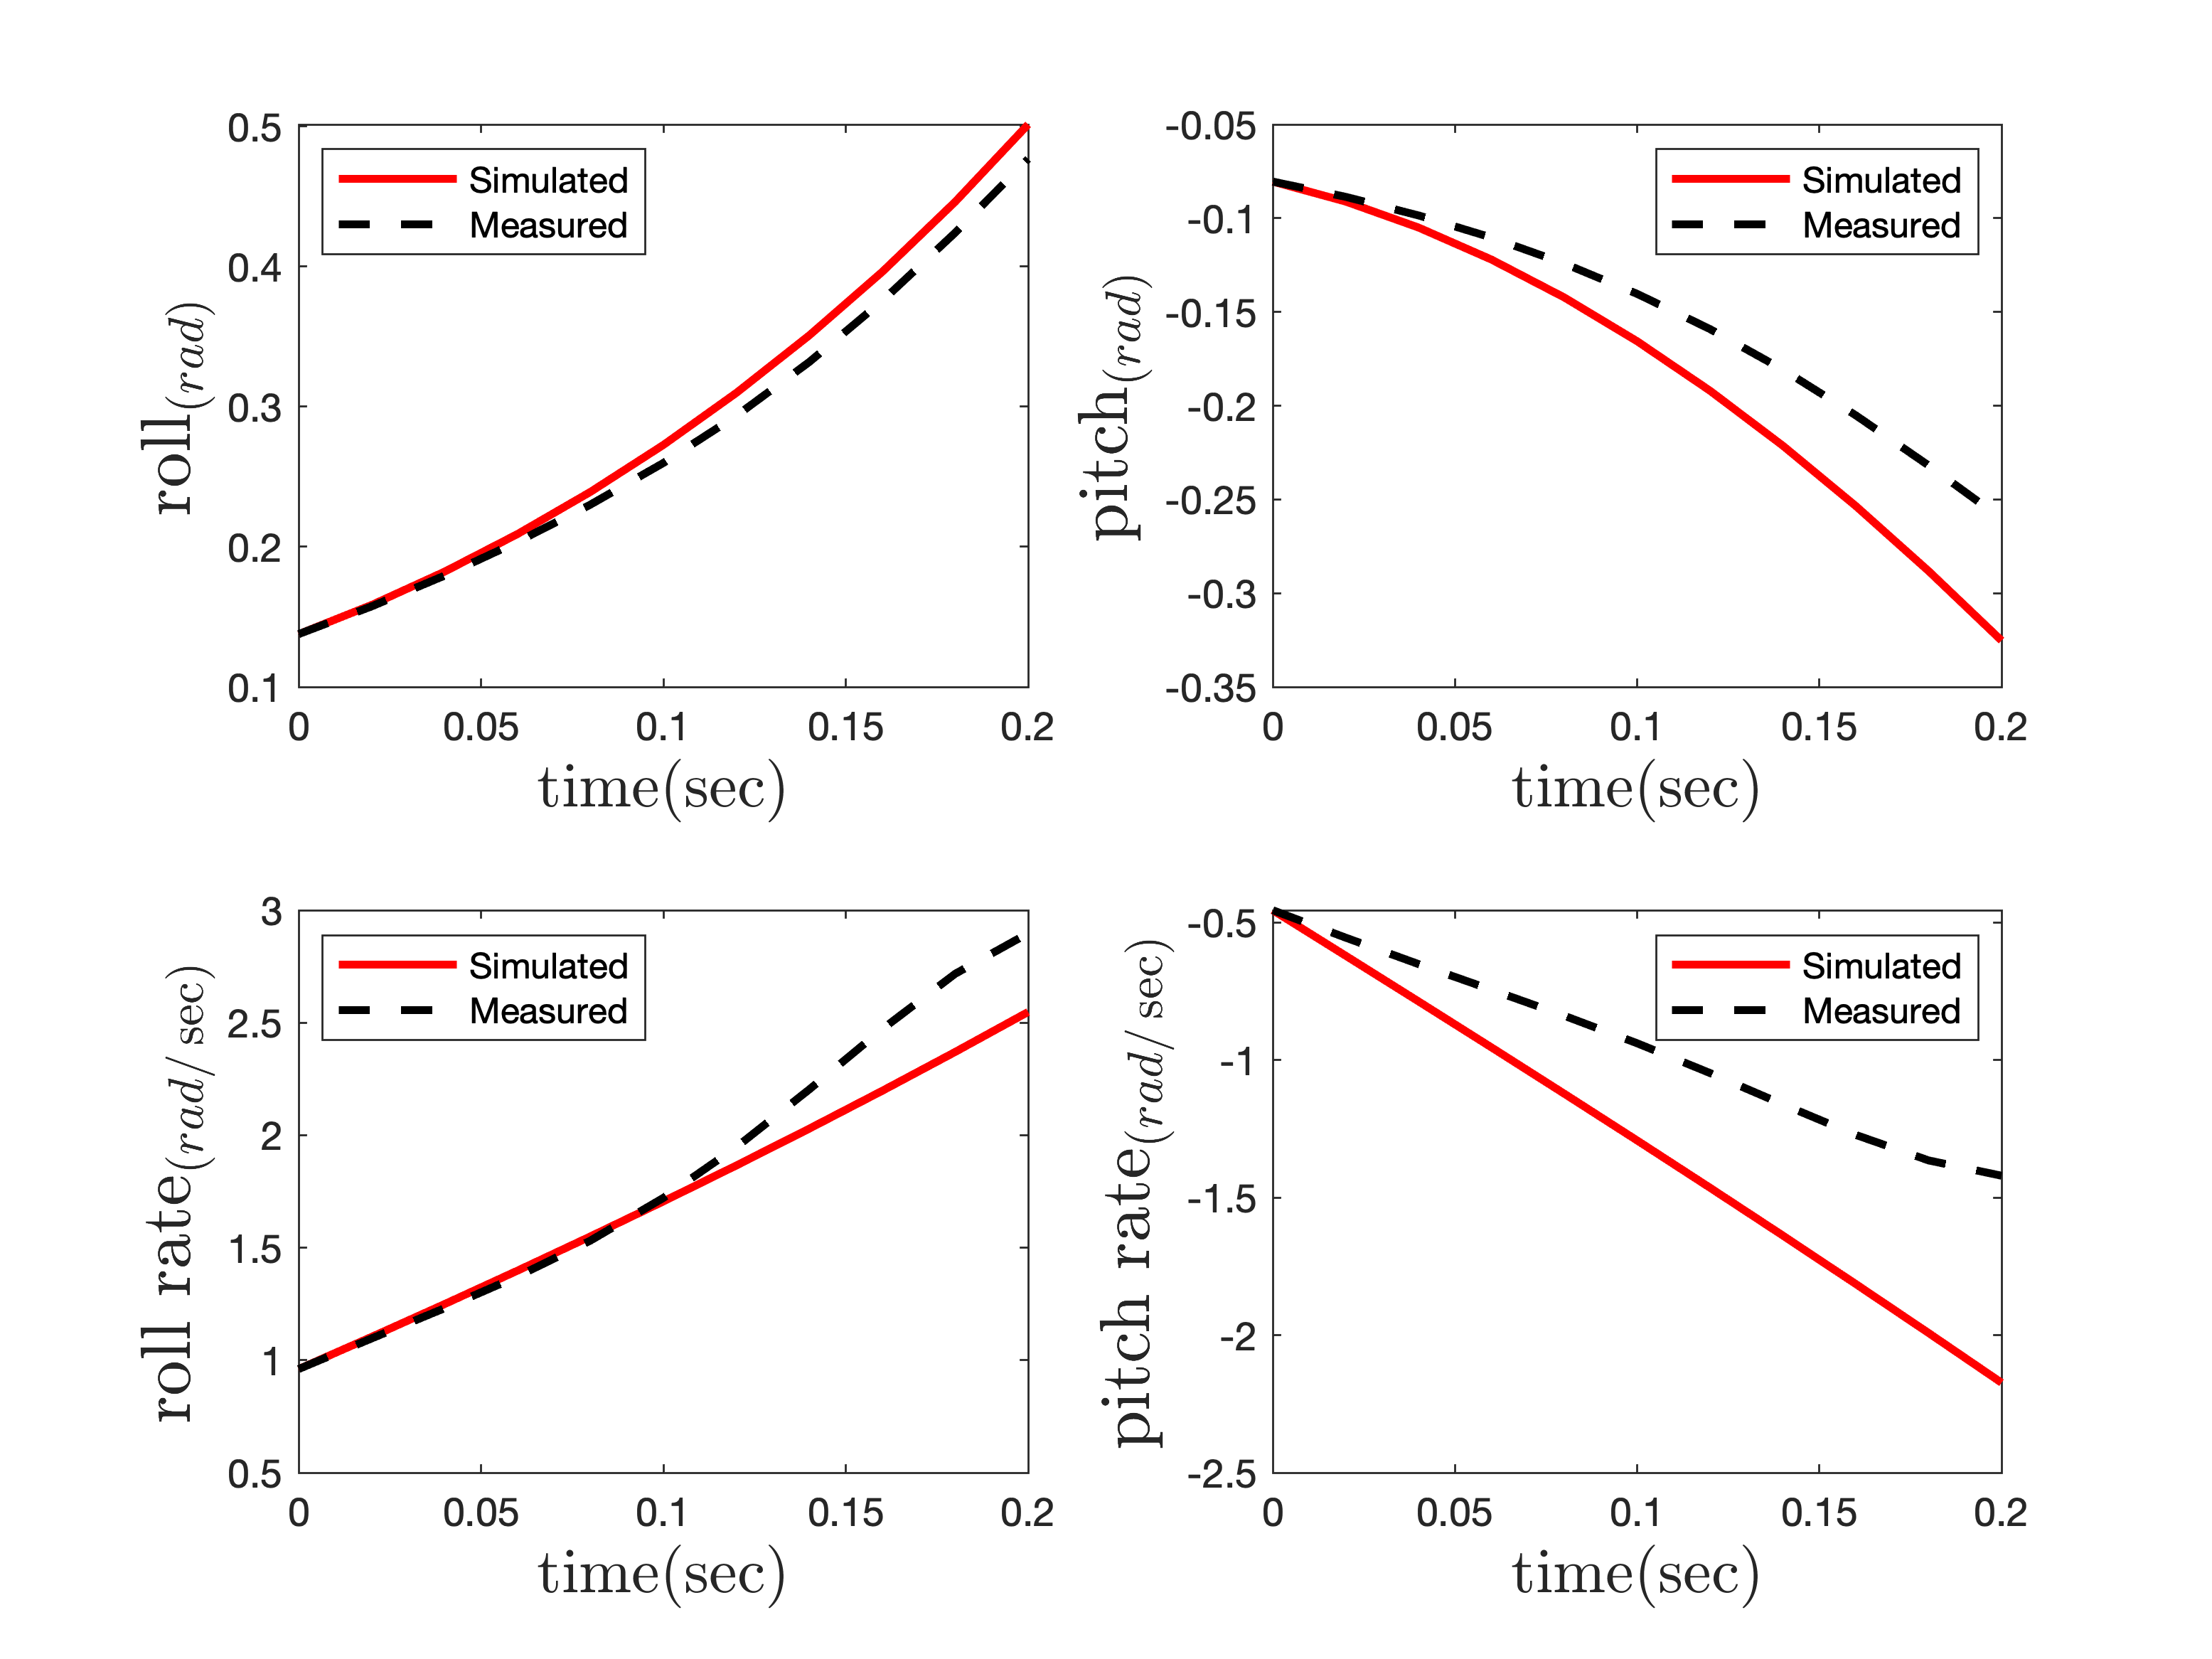
\includegraphics[width=12cm]{../../Figures/RCP/roll_pitch_parameter_estimation/RCP_roll_pitch_S4.png}
	\centering
	\caption{مقايسه وضعیت استند در  آزمايش چهارم و شبیه‌سازی، پس از تخمین پارامترهای کانال رول-پیچ}
	\label{roll_pitch_ps4}
\end{figure}
\begin{figure}[H]
	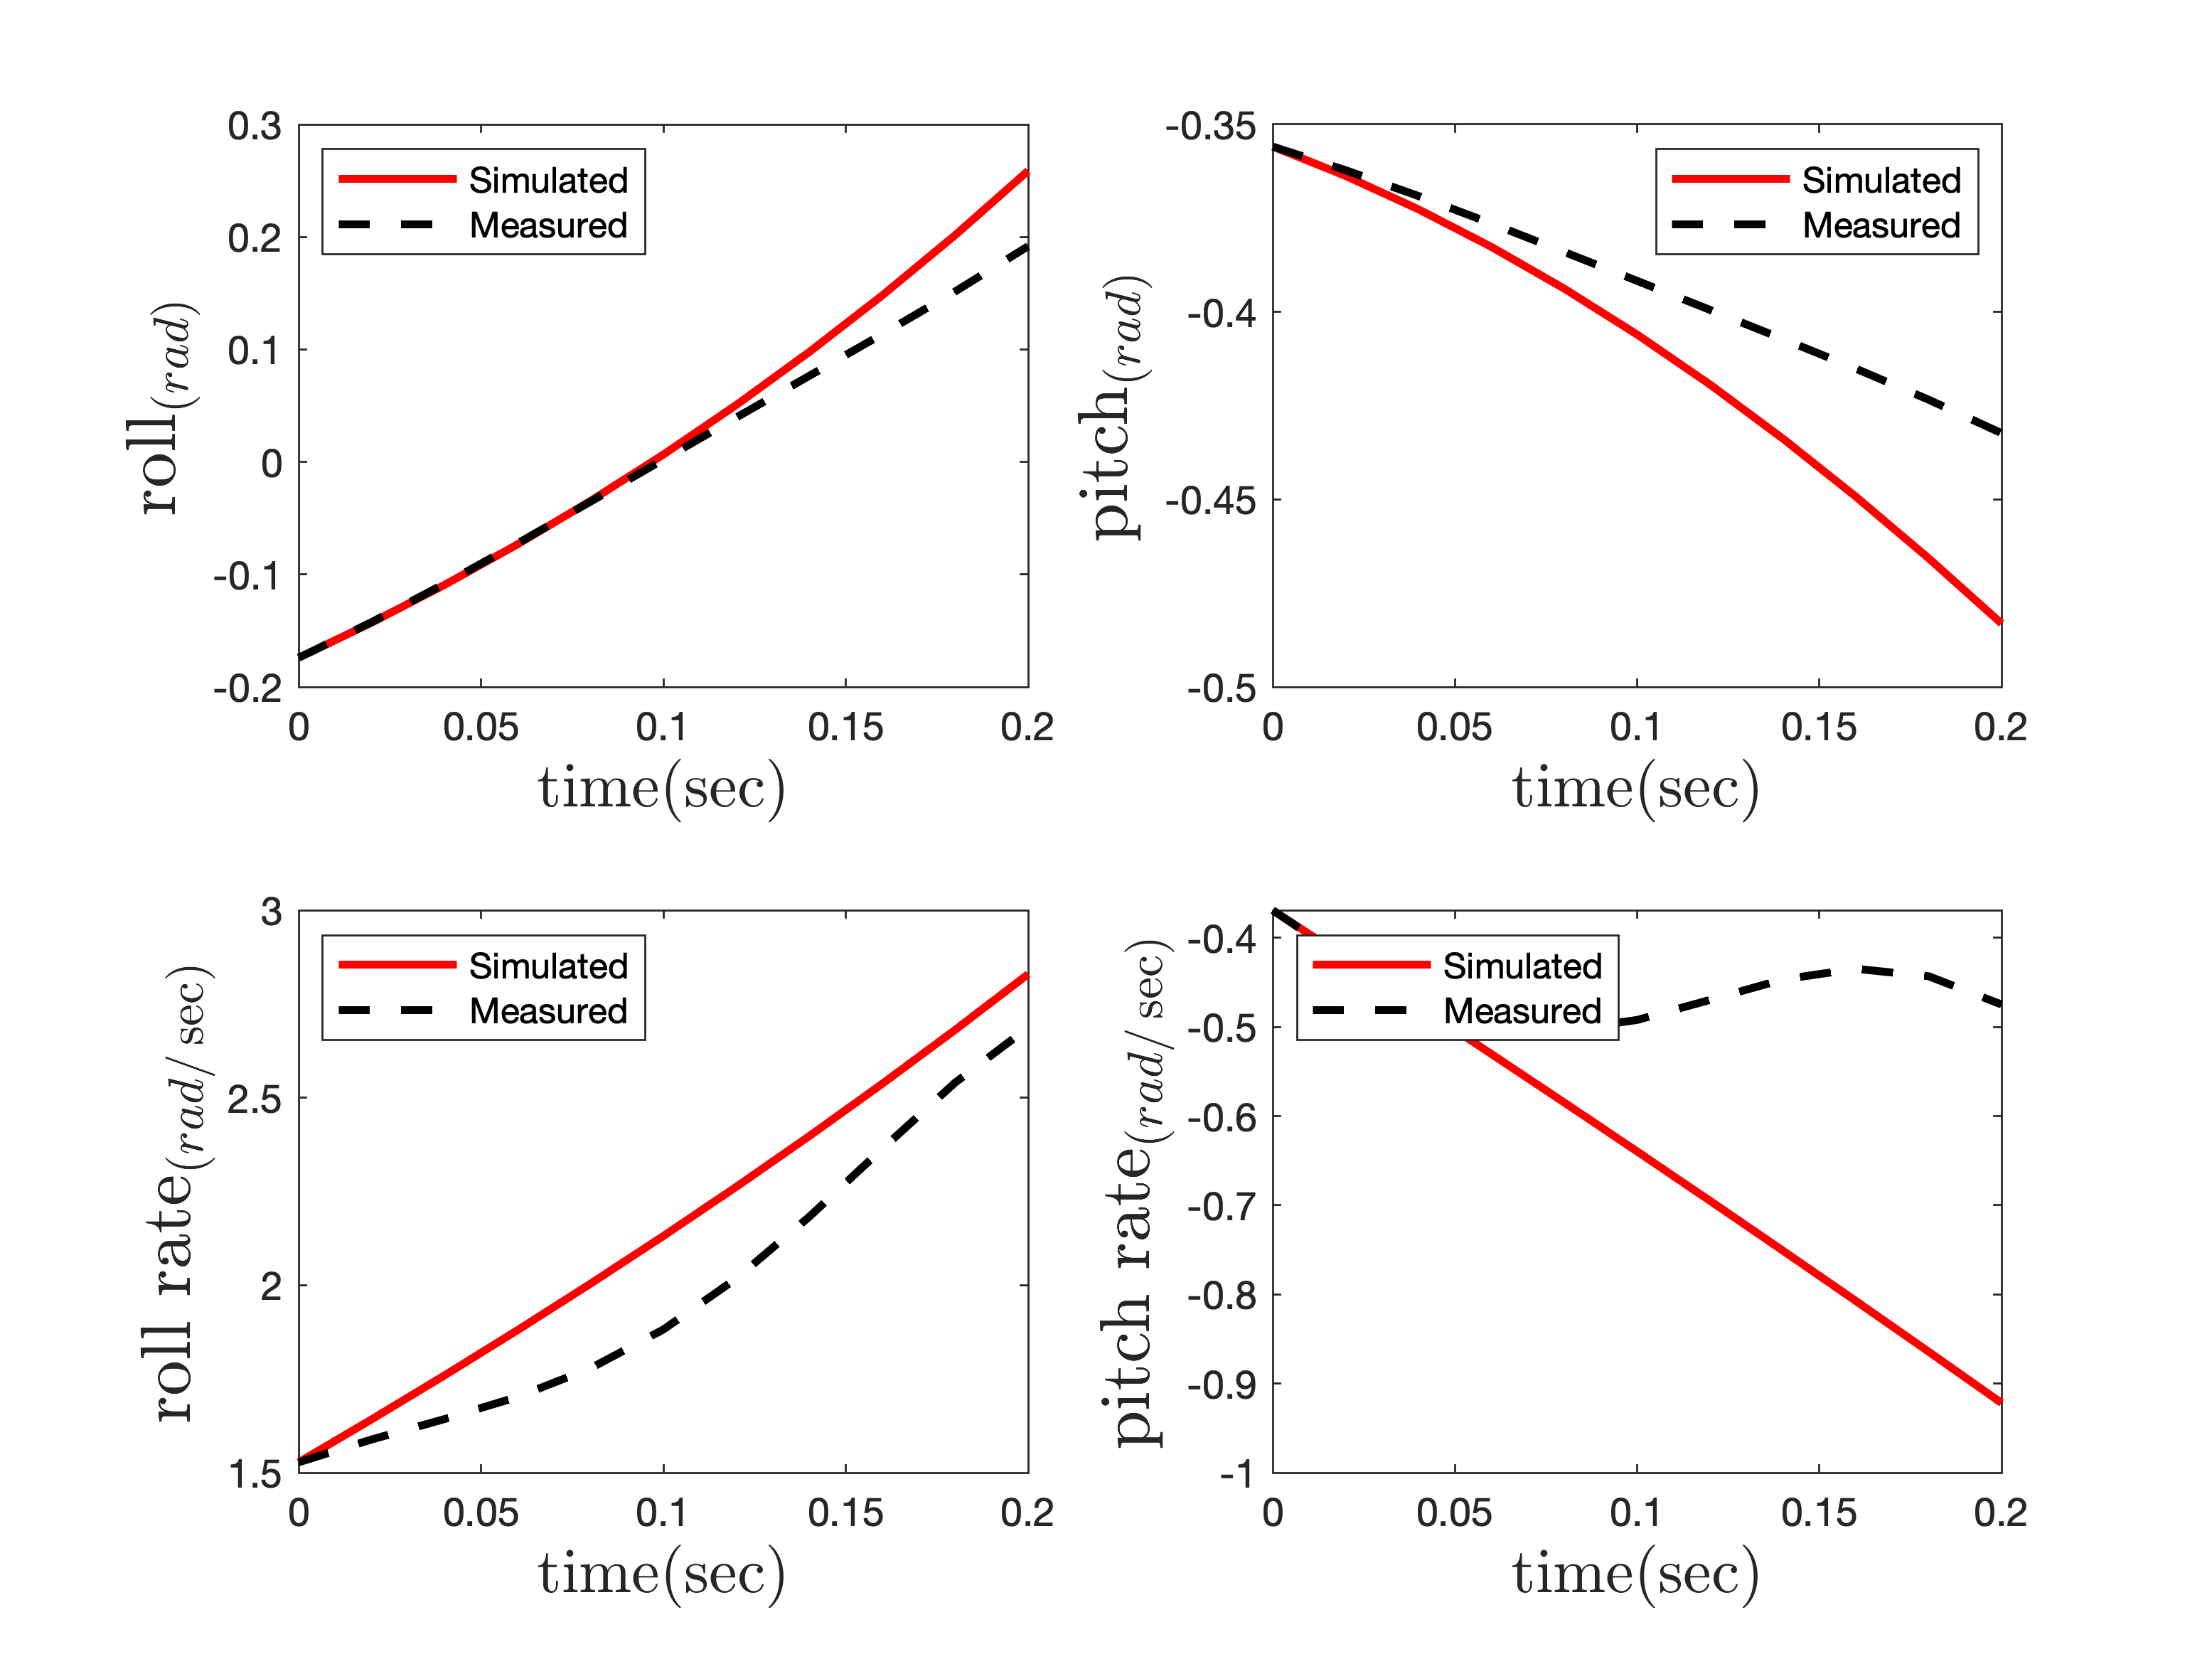
\includegraphics[width=12cm]{../../Figures/RCP/roll_pitch_parameter_estimation/RCP_roll_pitch_S5.png}
	\centering
	\caption{مقايسه وضعیت استند در  آزمايش پنجم و شبیه‌سازی، پس از تخمین پارامترهای کانال رول-پیچ}
	\label{roll_pitch_ps5}
\end{figure}
\begin{figure}[H]
	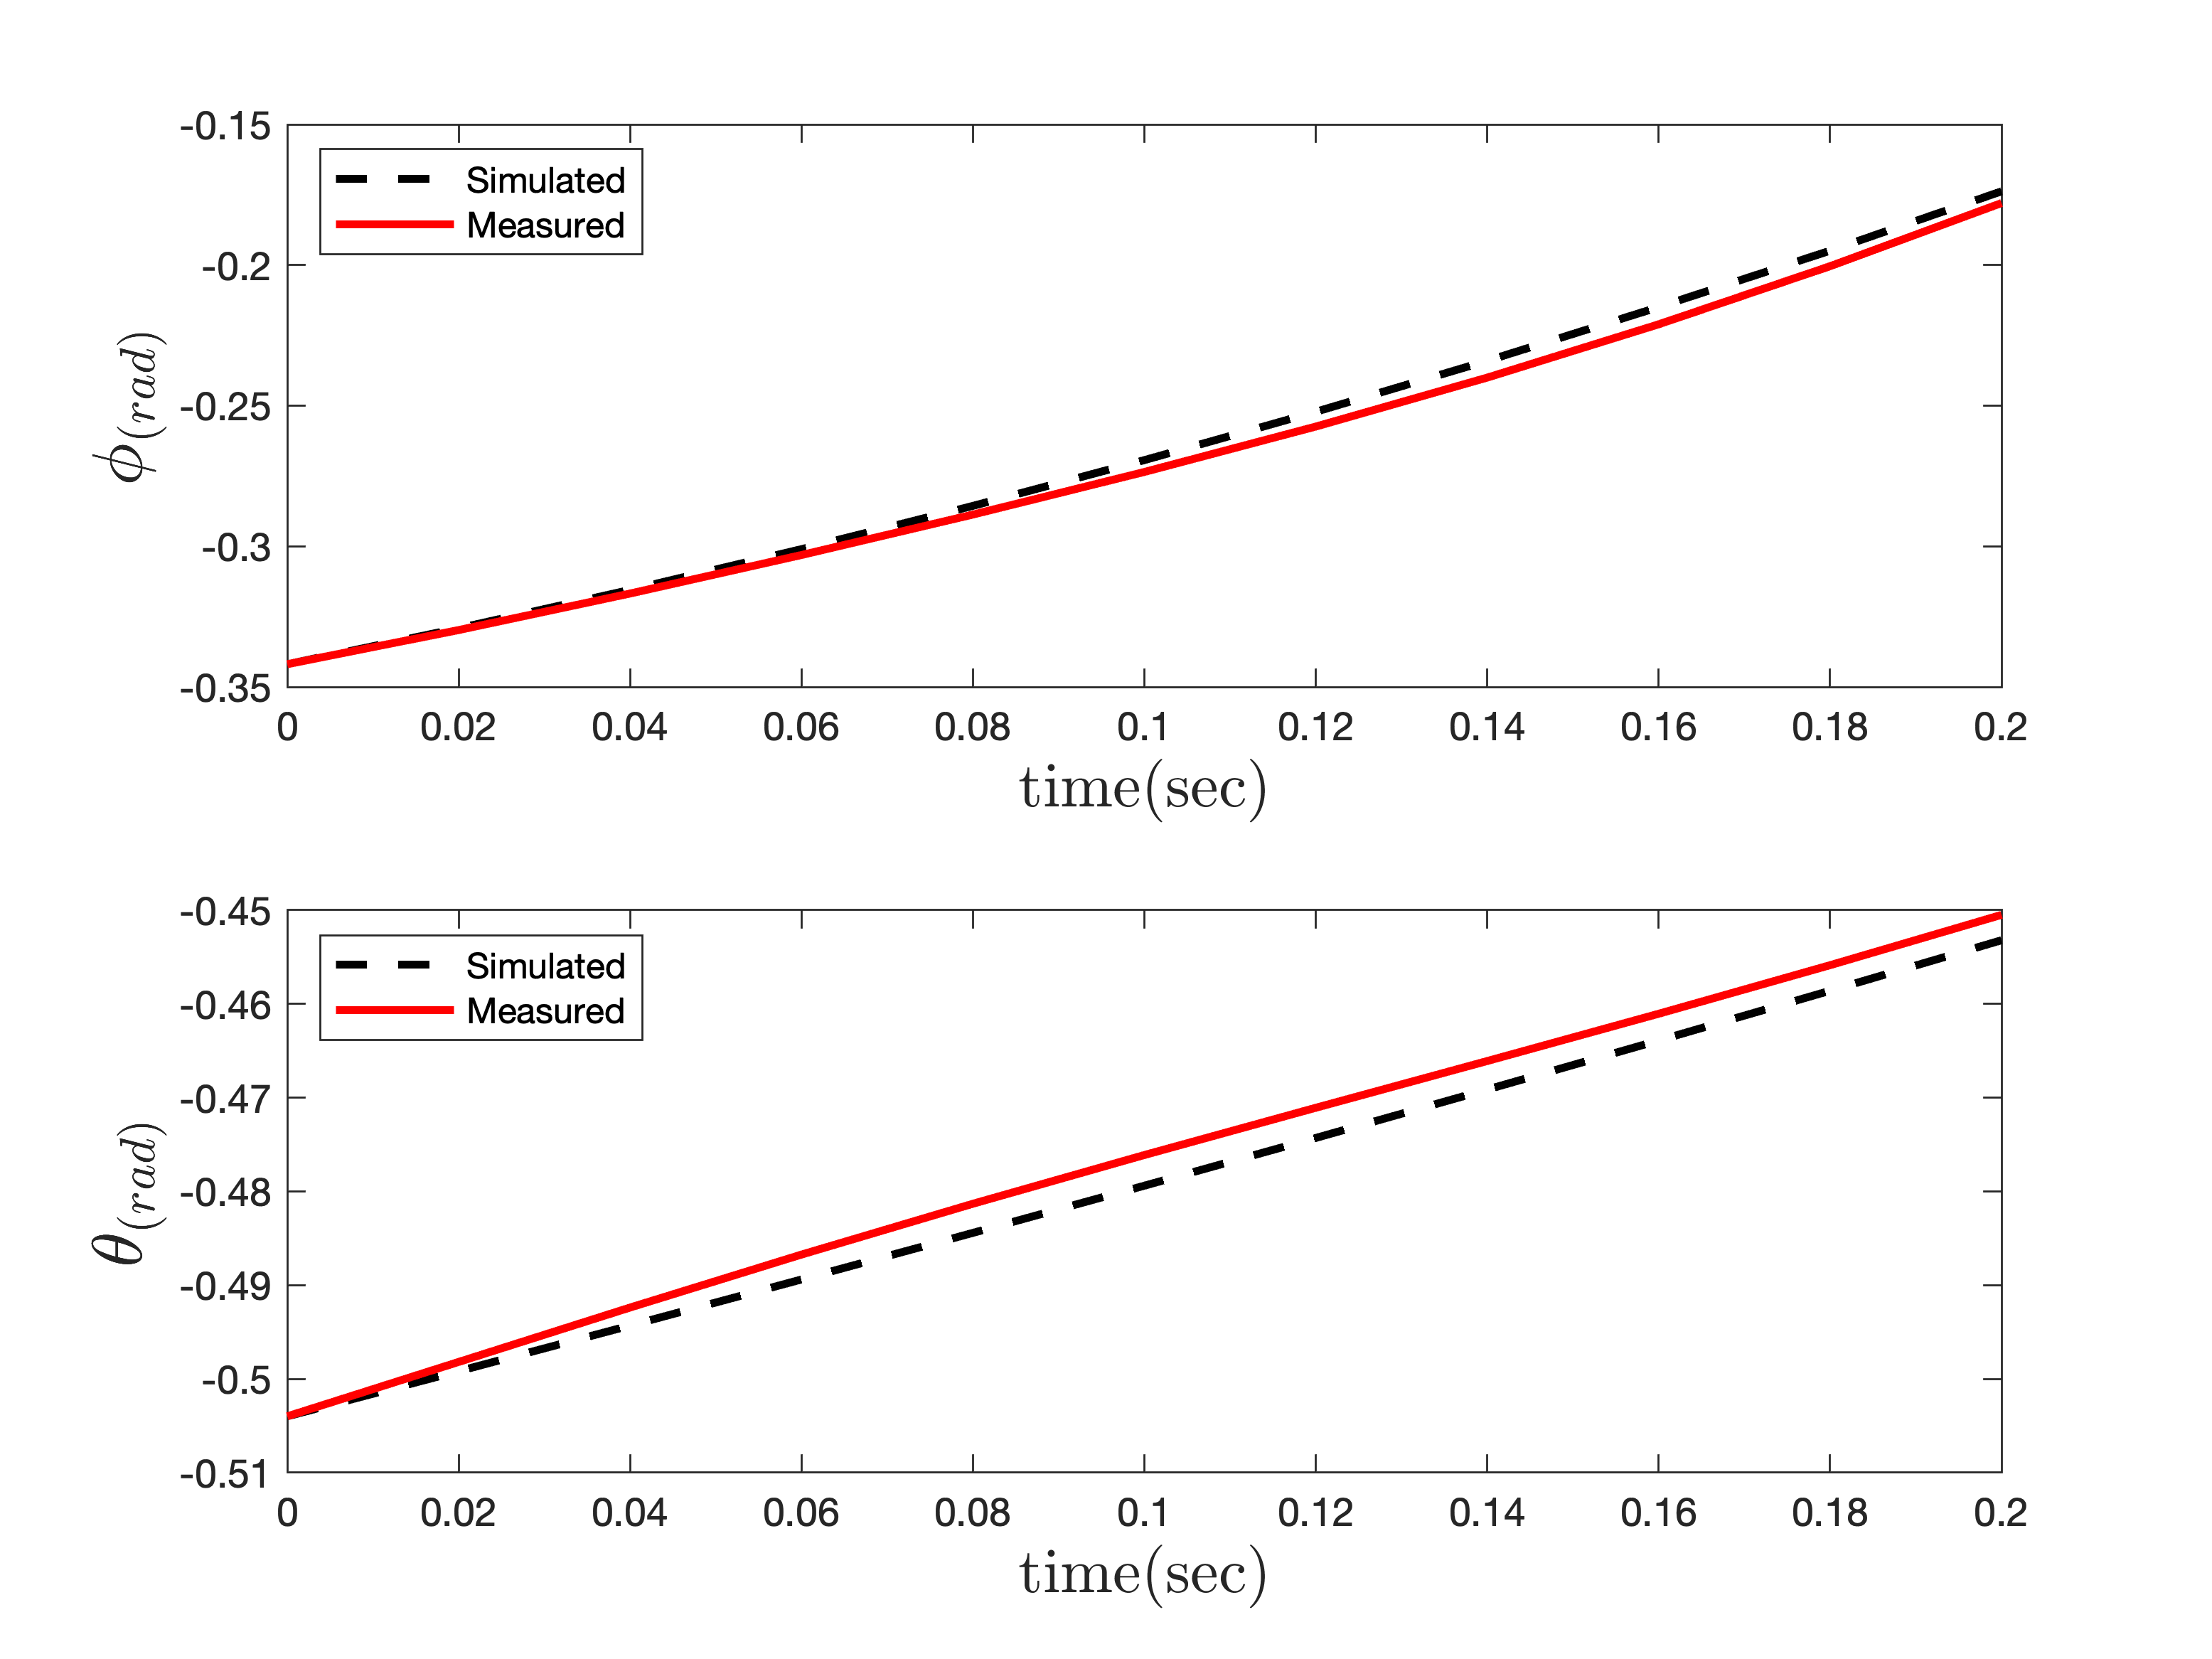
\includegraphics[width=12cm]{../../Figures/RCP/roll_pitch_parameter_estimation/RCP_roll_pitch_S6.png}
	\centering
	\caption{مقايسه وضعیت استند در  آزمايش ششم و شبیه‌سازی، پس از تخمین پارامترهای کانال رول-پیچ}
	\label{roll_pitch_ps6}
\end{figure}
\begin{figure}[H]
	\includegraphics[width=12cm]{../../Figures/RCP/roll_pitch_parameter_estimation/RCP_roll_pitch_S7.png}
	\centering
	\caption{مقايسه وضعیت استند در  آزمايش ششم و شبیه‌سازی، پس از تخمین پارامترهای کانال رول-پیچ}
	\label{roll_pitch_ps7}
\end{figure}
%\subsection{تخمین پارامتر کانال‌های رول-پیچ-یاو}
برای اصلاح پارامترها رول-پیچ چندین آزمایش انجام شد و با استفاده از داده‌های ثبت شده از وضعیت استند در کانال رول-پپچ-یاو و جعبه‌ابزار
\lr{Parameter Estimator}
پارامترهای کانال رول-پیچ-یاو اصلاح شدند.
برای آزمایش تمامی موتورها با دور مختلف شروع به حرکت کردند و از خروجی سنسور داده برداری شد. سپس، مدل و  داده‌های ثبت شده سنسور (وضعیت استند در کانال رول-پیج-یاو) به جعبه‌ابزار
\lr{Parameter Estimator}
داده شد. وضعیت کانال رول-پیچ-یاو استند در شبیه‌سازی و واقعیت بعد از اصلاح پارامترهای کانال‌ رول-پیچ-یاو بعد در شکل‌های
(\ref{ roll_pitch_yaw_ps1}, \ref{ roll_pitch_yaw_ps2}, \ref{ roll_pitch_yaw_ps3}, \ref{ roll_pitch_yaw_ps4}, \ref{ roll_pitch_yaw_ps5}, \ref{ roll_pitch_yaw_ps6}, \ref{ roll_pitch_yaw_ps7}, \ref{ roll_pitch_yaw_ps8}, \ref{ roll_pitch_yaw_ps9})
آورده شده است.

%\begin{figure}[H]
%	\includegraphics[width=12cm]{../Figures/RCP/roll_pitch_yaw_parameter_estimation/RCP_roll_pitch_yaw_S1.png}
%	\centering
%	\caption{مقايسه وضعیت استند در  آزمايش اول و شبیه‌سازی، پس از تخمین پارامترهای کانال رول-پیچ-یاو}
%	\label{ roll_pitch_yaw_ps1}
%\end{figure}
%\begin{figure}[H]
%	\includegraphics[width=12cm]{../Figures/RCP/roll_pitch_yaw_parameter_estimation/RCP_roll_pitch_yaw_S2.png}
%	\centering
%	\caption{مقايسه وضعیت استند در  آزمايش دوم و شبیه‌سازی، پس از تخمین پارامترهای کانال رول-پیچ-یاو}
%	\label{ roll_pitch_yaw_ps2}
%\end{figure}
%\begin{figure}[H]
%	\includegraphics[width=12cm]{../Figures/RCP/roll_pitch_yaw_parameter_estimation/RCP_roll_pitch_yaw_S3.png}
%	\centering
%	\caption{مقايسه وضعیت استند در  آزمايش سوم و شبیه‌سازی، پس از تخمین پارامترهای کانال رول-پیچ-یاو}
%	\label{ roll_pitch_yaw_ps3}
%\end{figure}
%\begin{figure}[H]
%	\includegraphics[width=12cm]{../Figures/RCP/roll_pitch_yaw_parameter_estimation/RCP_roll_pitch_yaw_S5.png}
%	\centering
%	\caption{مقايسه وضعیت استند در  آزمايش چهارم و شبیه‌سازی، پس از تخمین پارامترهای کانال رول-پیچ-یاو}
%	
%\end{figure}

\begin{figure}[H]
	\centering
	\subfigure[تغییرات زاویه رول]{
		\centering
		\includegraphics[width=.48\linewidth]{../Figures/RCP/roll_pitch_yaw_parameter_estimation/RCP_roll.png}
	}
	\subfigure[تغییرات زاویه پیچ]{
		\centering
		\includegraphics[width=.48\linewidth]{../Figures/RCP/roll_pitch_yaw_parameter_estimation/RCP_pitch.png}
	}
	\subfigure[تغییرات زاویه یاو]{
	\centering
	\includegraphics[width=.48\linewidth]{../Figures/RCP/roll_pitch_yaw_parameter_estimation/RCP_yaw.png}
}
	\caption{مقايسه وضعیت استند در  آزمايش چهارم و شبیه‌سازی، پس از تخمین پارامترهای کانال رول-پیچ-یاو}
	\label{ roll_pitch_yaw_ps4}
\end{figure}


%\begin{figure}[H]
%	\includegraphics[width=12cm]{../Figures/RCP/roll_pitch_yaw_parameter_estimation/RCP_roll_pitch_yaw_S6.png}
%	\centering
%	\caption{مقايسه وضعیت استند در  آزمايش پنجم و شبیه‌سازی، پس از تخمین پارامترهای کانال رول-پیچ-یاو}
%	\label{ roll_pitch_yaw_ps5}
%\end{figure}
%\begin{figure}[H]
%	\includegraphics[width=12cm]{../Figures/RCP/roll_pitch_yaw_parameter_estimation/RCP_roll_pitch_yaw_S7.png}
%	\centering
%	\caption{مقايسه وضعیت استند در  آزمايش ششم و شبیه‌سازی، پس از تخمین پارامترهای کانال رول-پیچ-یاو}
%	\label{ roll_pitch_yaw_ps6}
%\end{figure}
%\begin{figure}[H]
%	\includegraphics[width=12cm]{../Figures/RCP/roll_pitch_yaw_parameter_estimation/RCP_roll_pitch_yaw_S8.png}
%	\centering
%	\caption{مقايسه وضعیت استند در  آزمايش هفتم و شبیه‌سازی، پس از تخمین پارامترهای کانال رول-پیچ-یاو}
%	\label{ roll_pitch_yaw_ps7}
%\end{figure}
%\begin{figure}[H]
%	\includegraphics[width=12cm]{../Figures/RCP/roll_pitch_yaw_parameter_estimation/RCP_roll_pitch_yaw_S9.png}
%	\centering
%	\caption{مقايسه وضعیت استند در  آزمايش هشتم و شبیه‌سازی، پس از تخمین پارامترهای کانال رول-پیچ-یاو}
%	\label{ roll_pitch_yaw_ps8}
%\end{figure}
%\begin{figure}[H]
%	\includegraphics[width=12cm]{../Figures/RCP/roll_pitch_yaw_parameter_estimation/RCP_roll_pitch_yaw_S10.png}
%	\centering
%	\caption{مقايسه وضعیت استند در  آزمايش نهم و شبیه‌سازی، پس از تخمین پارامترهای کانال رول-پیچ-یاو}
%	\label{ roll_pitch_yaw_ps9}
%\end{figure}

%%------------ Controller------------------------
%%----------------MIL---------------------------
%\chapter{شبیه‌سازی استند سه درجه آزادی در حضور کنترل‌کننده}\label{MIL}
در بخش‌های
\ref{LQDG}
و
\ref{LQIDG}
کنترل‌کننده خطی مبتنی بر بازی دیفرانسیلی \lr{LQDG} و \lr{LQIDG} معرفی شد.در بخش‌های
\ref{roll_lqr_section_simulation}
و
\ref{roll_LQDG_section_simulation}
کانال 	رول چهارپره در حضور کنترل‌کننده‌های \lr{LQR} و
\lr{LQDG}
شبیه‌سازی می‌شود. سپس، در بخش‌های
\ref{roll_lqidg_section_simulation},
\ref{roll_pitch_lqidg_section_simulation}
و
\ref{roll_pitch_yaw_lqidg_section}
به‌ ترتیب شبیه‌سازی یک درجه آزادی، دو درجه آزادی و سه درجه آزادی در حضور کنترل‌کننده‌ \lr{LQIDG} انجام می‌شود.

\section{طراحی و شبیه‌سازی کنترل‌کننده برای کانال رول}\label{roll_lqr_section_simulation}
در بخش
\ref{quadall3}
شبیه‌سازی استند سه درجه آزادی چهارپره انجام شد.
در این بخش به کنترل زاویه رول با فرض مقید‌بودن زاویه پیچ و یاو پرداخته خواهد شد. به این منظور، در بخش
\ref{roll_regulator}
نتایج شبیه‌سازی برای تعقیب مقدار مطلوب خروجی زاویه رول ارائه می‌شود. سپس، در بخش
\ref{roll_noise}
عملکرد کنترل‌کننده در  حضور نویز اندازه‌گیری بررسی می‌شود.
\subsection{تعقیب مقدار مطلوب خروجی}\label{roll_regulator}


 در این بخش به ارائه مختصری از کنترل‌کننده \lr{LQR} پرداخته شده‌است. سپس، به بررسی عملکرد چهارپره در حضور کنترل‌کننده \lr{LQR} پرداخته می‌شود.
 برای یک سامانه خطی پیوسته با معادلات حالت:

\begin{equation}
	\begin{split}
		&\boldsymbol{\dot x}(t) = \boldsymbol{Ax}(t) + \boldsymbol{Bu}(t) %, \quad \boldsymbol{x}(0) = \boldsymbol{x}_0%
	\end{split}
\end{equation}
فرمان کنترلی بهینه \lr{LQR} به‌صورت زیر محاسبه می‌شود
\cite{ogata2010modern}:
\begin{equation}
		\boldsymbol{u_i}(t) = -\boldsymbol{K_{LQR}}\boldsymbol{x}(t)
\end{equation}
که در رابطه فوق، ماتریس $\boldsymbol{K_{LQR}}$ بیانگر بهره بازخورد بهینه است. این بهره به‌گونهای محاسبه می‌شود که تابع هزینه مربعی زیر کمینه شود:
 \begin{equation}\label{lqr_cost}
	J_i(u_1, u_2) = \int_{0}^{T}\left( \boldsymbol{x} ^\mathrm{T}(t) \boldsymbol{Q} \boldsymbol{x}(t)+
	\boldsymbol{u} ^\mathrm{T}(t) \boldsymbol{R} \boldsymbol{u}(t)
	\right)dt
	%	\boldsymbol{ x} ^\mathrm{T}(T)\boldsymbol{ H_i}\boldsymbol{x}(T) 
\end{equation}
در رابطه فوق، ماتریس‌های $Q$ و $R$ به ترتیب بیانگر میزان اهمیت انحراف متغیرهای حالت از مقادیر مطلوب و میزان تلاش کنترلی هستند. برای کمینه‌کردن رابطه
(\ref{lqr_cost})،
از رابطه زیر حاصل می‌شود:
\begin{equation}
	\boldsymbol{K_{LQR}} = \boldsymbol{R}^{-1}\boldsymbol{B}^\mathrm{T}\boldsymbol{P}
\end{equation}
در رابطه فوق، ماتریس $\boldsymbol{P}$ بیانگر پاسخ معادله ریكاتی زیر است:
\begin{equation}
	\boldsymbol{\dot{P}}(t) = \boldsymbol{A}^\mathrm{T} \boldsymbol{P}(t)  + \boldsymbol{P}(t) \boldsymbol{A} - \boldsymbol{P}(t) \boldsymbol{B} \boldsymbol{R}^{-1}\boldsymbol{B}^\mathrm{T} \boldsymbol{P}(t) + \boldsymbol{Q}
\end{equation}


 
 
  در شبیه‌سازی برای بهینه‌سازی ضرایب وزنی \lr{LQR} از روش بهینه‌سازی
\lr{TCACS}\LTRfootnote{Tabu Continuous Ant Colony System} \cite{Karimi2010}
استفاده شده‌است.
تابع هزینه \lr{TCACS} به‌صورت
\lr{ITSE}\LTRfootnote{Integral Time Square Error}
در نظر گرفته شده‌است. ضرایب وزنی خروجی بهینه‌سازی در پایین آورده شده‌است.
\begin{equation}
	\boldsymbol{Q_{LQR}} = \begin{bmatrix}
		0.5215 & 0\\
		0 & 0.0745
	\end{bmatrix}, \quad R_{LQR} =  0.0001
\end{equation} 
\begin{figure}[H]
	\includegraphics[width=.48\linewidth]{../Figures/MIL/LQR/Roll/lqr_roll_nn.png}
	\centering
	\caption{عملكرد \lr{LQR} در کنترل زاويه رول (تعقیب ورودی صفر)}
	\label{lqr_roll_figure_simulation}
\end{figure}
\begin{figure}[H]
	\centering
	\subfigure[موتور شماره دو]{
		\centering
		\includegraphics[width=.45\linewidth]{../Figures/MIL/LQR/Roll/lqr_roll_Omega_2_nn.png}
	}
	\subfigure[موتور شماره چهار]{
		\centering
		\includegraphics[width=.45\linewidth]{../Figures/MIL/LQR/Roll/lqr_roll_Omega_4_nn.png}
	}
	\caption{‫‪فرمان کنترلی موتورها در کنترل زاویه رول (تعقیب ورودی صفر)}
\end{figure}


بر اساس خروجی شبیه‌سازی (شکل
\ref{lqr_roll_figure_simulation})،
کانال رول در حضور کنترل‌کننده \lr{LQR} در حدود پنج ثانیه به تعادل می‌رسد اما دارای خطای ماندگار است. 
\section{شبیه‌سازی کانال رول استند در حضور کنترل‌کننده \lr{LQDG}}\label{roll_LQDG_section_simulation}
در بخش
\ref{quadchanell_roll}
شبیه‌سازی کانال رول استند چهارپره انجام شد. در این بخش به بررسی عملکرد چهارپره در حضور کنترل‌کننده \lr{LQDG} پرداخته می‌شود. کنترل‌کننده \lr{LQDG} در بخش
\ref{LQDG}
بررسی شده است.
 در شبیه‌سازی برای بهینه‌سازی ضرایب وزنی \lr{LQDG} از روش بهینه‌سازی
\lr{TCACS} \cite{Karimi2010}
استفاده شده است.
\begin{figure}[H]
	\includegraphics[width=.48\linewidth]{../Figures/MIL/LQDG/Roll/lqdg_roll.png}
	\centering
	\caption{عملكرد کنترل‌کننده \lr{LQDG} در کنترل زاويه رول (تعقیب ورودی صفر)}
	\label{lqdg_roll_fig_simulation}
\end{figure}
\begin{figure}[H]
	\centering
	\subfigure[موتور شماره دو]{
		\centering
		\includegraphics[width=.45\linewidth]{../Figures/MIL/LQDG/Roll/lqdg_roll_Omega_2.png}
	}
	\subfigure[موتور شماره چهار]{
		\centering
		\includegraphics[width=.45\linewidth]{../Figures/MIL/LQDG/Roll/lqdg_roll_Omega_4.png}
	}
	\caption{‫‪فرمان کنترلی موتورها در کنترل زاویه رول (تعقیب ورودی صفر)}
\end{figure}

بر اساس خروجی شبیه‌سازی (شکل
\ref{lqdg_roll_fig_simulation})،
کانال رول در حضور کنترل‌کننده \lr{LQDG} در کمتر از پنج ثانیه به تعادل می‌رسد اما دارای خطای ماندگار است ولی خطای 
مانگار آن نسبت به کنترل‌کننده
\lr{LQR}
بخش
\ref{roll_lqr_section_simulation}
کمتر است. به دلیل خطای ماندگار، در بخش
\ref{roll_lqidg_section_simulation}
انتگرال‌گیر به کنترل‌کننده اضافه می‌شود تا خطای ماندگار استند را کم کند.

\section{شبیه‌سازی کانال رول استند در حضور کنترل‌کننده \lr{LQIDG}}\label{roll_lqidg_section_simulation}
در بخش
\ref{quadchanell_roll}
شبیه‌سازی کانال رول استند چهارپره انجام شد. در این بخش به بررسی عملکرد چهارپره در حضور کنترل‌کننده \lr{LQIDG} پرداخته می‌شود. کنترل‌کننده \lr{LQIDG} در بخش
\ref{LQIDG}
بررسی شده‌است.
 در شبیه‌سازی برای بهینه‌سازی ضرایب وزنی \lr{LQIDG} از روش بهینه‌سازی
\lr{TCACS} \cite{Karimi2010}
استفاده شده است.
\begin{figure}[H]
	\includegraphics[width=.48\linewidth]{../Figures/MIL/LQIDG/Roll/lqidg_roll.png}
	\centering
	\caption{عملكرد \lr{LQIDG} در کنترل زاويه رول (تعقیب ورودی صفر)}
	\label{lqidg_roll_fig_simulation}
\end{figure}
\begin{figure}[H]
	\centering
	\subfigure[موتور شماره دو]{
		\centering
		\includegraphics[width=.45\linewidth]{../Figures/MIL/LQIDG/Roll/lqidg_roll_Omega_2.png}
	}
	\subfigure[موتور شماره چهار]{
		\centering
		\includegraphics[width=.45\linewidth]{../Figures/MIL/LQIDG/Roll/lqidg_roll_Omega_4.png}
	}
	\caption{‫‪فرمان کنترلی موتورها در کنترل زاویه رول (تعقیب ورودی صفر)}
\end{figure}

بر اساس خروجی شبیه‌سازی (شکل
\ref{lqidg_roll_fig_simulation})،
کانال رول در حضور کنترل‌کننده \lr{LQIDG} در حدود پنج ثانیه به تعادل می‌رسد و خطای ماندگار آن به دلیل وجود انتگرال‌گیر در حدود صفر است.
\section{پیاده‌سازی کنترل‌کننده برای کنترل کانال رول-پیچ}\label{roll_pitch_lqidg_section}
%در بخش
%\ref{roll_pitch_lqidg_section_simulation}
%شبیه‌سازی کانال رول-پیچ استند چهارپره در حضور کنترل‌کننده \lr{LQIDG} انجام شد. 
در این بخش به پیاده‌سازی کنترل‌کننده \lr{LQIDG} بر رویه کانال رول-پیچ استند سه درجه آزادی پرداخته می‌شود.
در پیاده‌سازی از ضرایب وزنی بهینه به دست آمده در قسمت شبیه‌سازی استفاده شده‌است.

\begin{figure}[H]
	\centering
	\subfigure[تغییرات زاویه رول]{
		\centering
		\includegraphics[width=.48\linewidth]{../Figures/Calibration/LQIDG/Roll_Pitch/lqidg_roll.png}
	}
	\subfigure[تغییرات زاویه پیچ]{
		\centering
		\includegraphics[width=.48\linewidth]{../Figures/Calibration/LQIDG/Roll_Pitch/lqidg_pitch.png}
	}
	\caption{‫‪عملکرد کنترل‌کننده \lr{LQIDG} در کنترل زاویه رول و پیچ (تعقیب ورودی صفر)}
\end{figure}

\begin{figure}[H]
	\centering
	\subfigure[موتور شماره یک]{
		\centering
		\includegraphics[width=.45\linewidth]{../Figures/Calibration/LQIDG/Roll_Pitch/lqidg_Omega_1.png}
	}
	\subfigure[موتور شماره دو]{
		\centering
		\includegraphics[width=.45\linewidth]{../Figures/Calibration/LQIDG/Roll_Pitch/lqidg_Omega_2.png}
	}
	\subfigure[موتور شماره سه]{
		\centering
		\includegraphics[width=.45\linewidth]{../Figures/Calibration/LQIDG/Roll_Pitch/lqidg_Omega_3.png}
	}
	\subfigure[موتور شماره چهار]{
		\centering
		\includegraphics[width=.45\linewidth]{../Figures/Calibration/LQIDG/Roll_Pitch/lqidg_Omega_4.png}
	}
	\caption{‫‪فرمان کنترلی موتورها در کنترل زاویه رول و پیچ (تعقیب ورودی صفر)}
\end{figure}






%بر اساس خروجی شبیه‌سازی (شکل
%\ref{lqidg_roll_fig})
%،کانال رول در حضور کنترل‌کننده \lr{LQIDG} در حدود پنج ثانیه و کانال پیچ در حدود هشت ثانیه به تعادل می‌رسد و خطای ماندگار آن در حدود صفر است.
\section{طراحی و شبیه‌سازی کنترل‌کننده برای کانال رول-پیچ-یاو}\label{roll_pitch_yaw_lqidg_section}
در بخش
\ref{quadall3}
شبیه‌سازی سه درجه آزادی استند چهارپره انجام شد. در این بخش به بررسی عملکرد چهارپره در حضور کنترل‌کننده \lr{LQIDG} پرداخته می‌شود. کنترل‌کننده \lr{LQIDG} در بخش‌های
\ref{LQIDG}
بررسی شده است.
 در شبیه‌سازی برای بهینه‌سازی ضرایب وزنی \lr{LQIDG} از روش بهینه‌سازی
\lr{TCACS} \cite{Karimi2010}
استفاده شده‌است.
تابع هزینه \lr{TCACS} به‌صورت
\lr{ITSE}
در نظر گرفته شده‌است. ضرایب وزنی خروجی بهینه‌سازی در پایین آورده شده‌است. برای طراحی کنترل‌کننده
\lr{LQIDG}
ضرایب وزنی
$R_1$
و
$R_2$
برای کانال‌های مختلف یکی فرض شده‌است.
\subsection{شبیه‌سازی کنترل‌کننده به‌صورت سه کانال تک ورودی}


\begin{equation*}
	\begin{split}
				&\boldsymbol{Q_{a_{LQIDG_{roll}}}} = \begin{bmatrix}
			631.85 & 0.00 & 0.00 & 0.00  \\ 
			0.00 & 214.28 & 0.00 & 0.00  \\ 
			0.00 & 0.00 & 7.91 & 0.00  \\ 
			0.00 & 0.00 & 0.00 & 0.01  \\ 
		\end{bmatrix} ,
		\boldsymbol{Q_{a_{LQIDG_{pitch}}}} = \begin{bmatrix}
			0.01 & 0.00 & 0.00 & 0.00  \\
			0.00 & 873.93 & 0.00 & 0.00  \\ 
			0.00 & 0.00 & 9853.09 & 0.00 \\ 
			0.00 & 0.00 & 0.00 & 0.12  \\ 
		\end{bmatrix}\\
			&\boldsymbol{Q_{a_{LQIDG_{yaw}}}}  = \begin{bmatrix}
0.03 & 0.00 & 0.00 & 0.00 & \\ 
0.00 & 0.17 & 0.00 & 0.00 & \\ 
0.00 & 0.00 & 1.81 & 0.00 & \\ 
0.00 & 0.00 & 0.00 & 33333.45 & \\
	\end{bmatrix}\times 10^{-4}, \quad R_{1_{LQDG}} = 1, \quad R_{2_{LQDG}} = 1.2577
	\end{split}
\end{equation*}

در گام بعد، با حل معادله
(\ref{coupled_riccatti_LQIDG})
(برای سادگی ماتریس‌های وزنی $\boldsymbol{\dot{Q}_{a_2}}$ و $\boldsymbol{\dot{Q}_{a_1}}$مساوی در نظر گرفته شده‌است)
ماتریس
$\boldsymbol{\dot{K}_1}$
به‌صورت زیر به دست می‌آید.
\begin{equation}
	\begin{split}
			\boldsymbol{K_{a_{1_{roll}}}} &= \begin{bmatrix}
435.89 & 20.54 & 42.44 & -9.98 \\ 
20.54 & 11.93 & 1.98 & -0.00 \\ 
42.44 & 1.98 & 71.49 & -0.08 \\ 
-9.98 & -0.00 & -0.08 & 9.93 \\ 
		\end{bmatrix}, \boldsymbol{K_{a_{1_{pitch}}}} \begin{bmatrix}
2430.43 & 59.59 & 3128.26 & -11.75 \\ 
59.59 & 23.52 & 74.08 & 0.00 \\ 
3128.26 & 74.08 & 7851.78 & -0.12 \\ 
-11.75 & 0.00 & -0.12 & 11.75 \\ 
		\end{bmatrix}\\
\boldsymbol{K_{a_{1_{yaw}}}} &= 
\begin{bmatrix}
57.75 & 1.46 & 3.56 & -54.52 \\ 
1.46 & 1.27 & 0.10 & -0.00 \\ 
3.56 & 0.10 & 0.24 & -3.34 \\ 
-54.52 & -0.00 & -3.34 & 54.51 \\ 
\end{bmatrix}\\
	\end{split}
\end{equation}

در نهایت فرمان کنترلی بهینه بازیکن اول از رابطه
(\ref{LQIDG_u})
به‌صورت زیر به دست می‌آید.
\begin{equation}
	\begin{split}
		u_{1_{roll}} &= -\begin{bmatrix}
			20.5410 & 11.9267 & 1.9771 & 0.0021
		\end{bmatrix} \boldsymbol{x_{a_{roll}}} \\
		u_{1_{pitch}} &= -\begin{bmatrix}
			59.5923 & 23.5197 & 74.0822 & 0.000
		\end{bmatrix} \boldsymbol{x_{a_{pitch}}} \\
	u_{1_{yaw}} &= -\begin{bmatrix}
		1.45710 & 1.27300 & 0.0999 & 0.0041
	\end{bmatrix} \boldsymbol{x_{a_{yaw}}} 
	\end{split}
\end{equation}
%\begin{figure}[H]
%	\centering
%	\begin{subfigure}[H]
%		\centering
%		\includegraphics[width=12cm]{../Figures/MIL/LQIDG/3DOF/lqidg_roll.png}
%		\caption{تغییرات زاویه رول}
%	\end{subfigure}%
%	\begin{subfigure}
%		\centering
%		\includegraphics[width=12cm]{../Figures/MIL/LQIDG/3DOF/lqidg_pitch.png}
%		\caption{تغییرات زاویه پیچ}
%	\end{subfigure}
%	\caption{‫‪عملکرد کنترل‌کننده LQIDG در کنترل زاویه رول، پیچ و یاد (تعقیب ورودی صفر)}
%\end{figure}
%
%\begin{figure}[H]
%	\centering
%	\begin{subfigure}[H]
%		\centering
%		\includegraphics[width=12cm]{../Figures/MIL/LQIDG/3DOF/lqidg_yaw.png}
%		\caption{تغییرات زاویه یاو}
%	\end{subfigure}
%	\caption{‫‪عملکرد کنترل‌کننده LQIDG در کنترل زاویه رول، پیچ و یاد (تعقیب ورودی صفر)}
%\end{figure}
\begin{figure}[H]
	\centering
\subfigure[تغییرات زاویه رول]{
	\centering
	\includegraphics[width=.48\linewidth]{../Figures/MIL/LQIDG/3DOF/lqidg_roll_nn.png}
}
\subfigure[تغییرات زاویه پیچ]{
	\centering
	\includegraphics[width=.48\linewidth]{../Figures/MIL/LQIDG/3DOF/lqidg_pitch_nn.png}
}
\subfigure[تغییرات زاویه یاو]{
	\centering
	\includegraphics[width=.48\linewidth]{../Figures/MIL/LQIDG/3DOF/lqidg_yaw_nn.png}
}
	\caption{‫‪عملکرد کنترل‌کننده \lr{LQIDG} در کنترل زاویه رول، پیچ و یاو (تعقیب ورودی صفر)}
	\label{lqidg_roll_pitch_yaw_fig_simulation}
\end{figure}


\begin{figure}[H]
	\centering
	\subfigure[موتور شماره یک]{
		\centering
		\includegraphics[width=.45\linewidth]{../Figures/MIL/LQIDG/3DOF/lqidg_roll_pitch_Omega_1_nn.png}
	}
	\subfigure[موتور شماره دو]{
		\centering
		\includegraphics[width=.45\linewidth]{../Figures/MIL/LQIDG/3DOF/lqidg_roll_pitch_Omega_2_nn.png}
	}
	\subfigure[موتور شماره سه]{
		\centering
		\includegraphics[width=.45\linewidth]{../Figures/MIL/LQIDG/3DOF/lqidg_roll_pitch_Omega_3_nn.png}
	}
	\subfigure[موتور شماره چهار]{
		\centering
		\includegraphics[width=.45\linewidth]{../Figures/MIL/LQIDG/3DOF/lqidg_roll_pitch_Omega_4_nn.png}
	}
	\caption{‫‪فرمان کنترلی موتورها در کنترل زاویه رول، پیچ و یاو (تعقیب ورودی صفر)}
\end{figure}

\subsection{شبیه‌سازی کنترل‌کننده به‌صورت چهار ورودی}
\setcounter{MaxMatrixCols}{20}


\begin{equation*}
	\boldsymbol{Q_{a_{LQIDG}}} = 
	\begin{bmatrix}
		631.85 & 0.00 & 0.00 & 0.00 & 0.00 & 0.00 & 0.00 & 0.00 & 0.00 & 0.00 & 0.00 & 0.00\\ 
		0.00 & 214.28 & 0.00 & 0.00 & 0.00 & 0.00 & 0.00 & 0.00 & 0.00 & 0.00 & 0.00 & 0.00\\ 
		0.00 & 0.00 & 7.91 & 0.00 & 0.00 & 0.00 & 0.00 & 0.00 & 0.00 & 0.00 & 0.00 & 0.00\\ 
		0.00 & 0.00 & 0.00 & 0.01 & 0.00 & 0.00 & 0.00 & 0.00 & 0.00 & 0.00 & 0.00 & 0.00\\ 
		0.00 & 0.00 & 0.00 & 0.00 & 0.01 & 0.00 & 0.00 & 0.00 & 0.00 & 0.00 & 0.00 & 0.00\\ 
		0.00 & 0.00 & 0.00 & 0.00 & 0.00 & 873.93 & 0.00 & 0.00 & 0.00 & 0.00 & 0.00 & 0.00\\ 
		0.00 & 0.00 & 0.00 & 0.00 & 0.00 & 0.00 & 9853.09 & 0.00 & 0.00 & 0.00 & 0.00 & 0.00\\ 
		0.00 & 0.00 & 0.00 & 0.00 & 0.00 & 0.00 & 0.00 & 0.12 & 0.00 & 0.00 & 0.00 & 0.00\\ 
		0.00 & 0.00 & 0.00 & 0.00 & 0.00 & 0.00 & 0.00 & 0.00 & 0.00 & 0.00 & 0.00 & 0.00\\ 
		0.00 & 0.00 & 0.00 & 0.00 & 0.00 & 0.00 & 0.00 & 0.00 & 0.00 & 0.00 & 0.00 & 0.00\\ 
		0.00 & 0.00 & 0.00 & 0.00 & 0.00 & 0.00 & 0.00 & 0.00 & 0.00 & 0.00 & 0.00 & 0.00\\ 
		0.00 & 0.00 & 0.00 & 0.00 & 0.00 & 0.00 & 0.00 & 0.00 & 0.00 & 0.00 & 0.00 & 3.33\\ 
		
	\end{bmatrix}
\end{equation*}

\begin{equation*}
	\begin{bmatrix}
		-0.00 & 101.23 & 5.33 & -0.00 & 48.29 & 45.40 & 0.00 & 0.07 & 0.34 & -0.00 & -0.00 & 0.15\\ 
		241.81 & -0.00 & -5.33 & 86.14 & -0.00 & -45.40 & 57.31 & 0.00 & -0.34 & 0.00 & -0.00 & -0.15\\ 
		-0.00 & -101.23 & 5.33 & -0.00 & -48.29 & 45.40 & 0.00 & -0.07 & 0.34 & -0.00 & 0.00 & 0.15\\ 
		-241.81 & -0.00 & -5.33 & -86.14 & -0.00 & -45.40 & -57.31 & 0.00 & -0.34 & -0.00 & -0.00 & -0.15\\ 
	\end{bmatrix}
\end{equation*}


\begin{equation*}
	\boldsymbol{K_{a_1}} = 
	\begin{bmatrix}
34004 & -0 & -0 & 11130 & -0 & -0 & 14810 & 0 & -0 & -9 & -0 & -0\\ 
-0 & 7396 & 0 & -0 & 3498 & 0 & 0 & 11 & 0 & -0 & -10 & 0\\ 
-0 & 0 & 1504 & -0 & 0 & 10019 & 0 & -0 & 95 & -0 & 0 & -27\\ 
11129 & -0 & -0 & 3965 & -0 & -0 & 2638 & 0 & -0 & 0 & -0 & -0\\ 
-0 & 3498 & 0 & -0 & 1669 & 0 & 0 & 3 & 0 & -0 & -0 & 0\\ 
-0 & 0 & 10019 & -0 & 0 & 85406 & 0 & -0 & 630 & -0 & 0 & 277\\ 
14810 & 0 & 0 & 2638 & 0 & 0 & 24372 & -0 & 0 & -0 & 0 & 0\\ 
0 & 11 & -0 & 0 & 3 & -0 & -0 & 11 & -0 & 0 & -0 & -0\\ 
-0 & 0 & 95 & -0 & 0 & 630 & 0 & -0 & 7 & -0 & 0 & -2\\ 
-10 & -0 & -0 & -0 & -0 & -0 & -0 & 0 & -0 & 10 & -0 & -0\\ 
-0 & -10 & 0 & -0 & -0 & 0 & 0 & -0 & 0 & -0 & 9 & 0\\ 
-0 & 0 & -27 & -0 & 0 & 277 & 0 & -0 & -2 & -0 & 0 & 59\\ 

	\end{bmatrix}
\end{equation*}



\begin{figure}[H]
	\centering
	\subfigure[تغییرات زاویه رول]{
		\centering
		\includegraphics[width=.48\linewidth]{../Figures/MIL/LQIDG/MIMO/lqidg_roll_nn.png}
	}
	\subfigure[تغییرات زاویه پیچ]{
		\centering
		\includegraphics[width=.48\linewidth]{../Figures/MIL/LQIDG/MIMO/lqidg_pitch_nn.png}
	}
	\subfigure[تغییرات زاویه یاو]{
		\centering
		\includegraphics[width=.48\linewidth]{../Figures/MIL/LQIDG/MIMO/lqidg_yaw_nn.png}
	}
	\caption{‫‪عملکرد کنترل‌کننده \lr{LQIDG} در کنترل زاویه رول، پیچ و یاو (تعقیب ورودی صفر)}
	\label{lqidg_roll_pitch_yaw_fig_simulation_MIMO}
\end{figure}


\begin{figure}[H]
	\centering
	\subfigure[موتور شماره یک]{
		\centering
		\includegraphics[width=.45\linewidth]{../Figures/MIL/LQIDG/MIMO/lqidg_roll_pitch_Omega1_nn.png}
	}
	\subfigure[موتور شماره دو]{
		\centering
		\includegraphics[width=.45\linewidth]{../Figures/MIL/LQIDG/MIMO/lqidg_roll_pitch_Omega2_nn.png}
	}
	\subfigure[موتور شماره سه]{
		\centering
		\includegraphics[width=.45\linewidth]{../Figures/MIL/LQIDG/MIMO/lqidg_roll_pitch_Omega3_nn.png}
	}
	\subfigure[موتور شماره چهار]{
		\centering
		\includegraphics[width=.45\linewidth]{../Figures/MIL/LQIDG/MIMO/lqidg_roll_pitch_Omega4_nn.png}
	}
	\caption{‫‪فرمان کنترلی موتورها در کنترل زاویه رول، پیچ و یاو (تعقیب ورودی صفر)}
\end{figure}
%%----------------Calibration---------------------------
\chapter{شبیه‌سازی استند سه درجه آزادی در حضور کنترل‌کننده}\label{MIL}
در بخش‌های
\ref{LQDG}
و
\ref{LQIDG}
کنترل‌کننده خطی مبتنی بر بازی دیفرانسیلی \lr{LQDG} و \lr{LQIDG} معرفی شد.در بخش‌های
\ref{roll_lqr_section_simulation}
و
\ref{roll_LQDG_section_simulation}
کانال 	رول چهارپره در حضور کنترل‌کننده‌های \lr{LQR} و
\lr{LQDG}
شبیه‌سازی می‌شود. سپس، در بخش‌های
\ref{roll_lqidg_section_simulation},
\ref{roll_pitch_lqidg_section_simulation}
و
\ref{roll_pitch_yaw_lqidg_section}
به‌ ترتیب شبیه‌سازی یک درجه آزادی، دو درجه آزادی و سه درجه آزادی در حضور کنترل‌کننده‌ \lr{LQIDG} انجام می‌شود.

\section{نتایج کنترل کانال پیچ}\label{roll_lqr_section}
%در بخش
%\ref{roll_lqr_section_simulation}
%شبیه‌سازی تک کانال استند چهارپره در حضور کنترل‌کننده \lr{LQR} انجام شد. در این بخش به پیاده‌سازی کنترل‌کننده \lr{LQR} برای کانال پیچ استند سه درجه آزادی پرداخته می‌شود. 
در پیاده‌سازی از ضرایب وزنی بهینه به دست آمده در قسمت شبیه‌سازی استفاده شده‌است.
\begin{figure}[H]
	\includegraphics[width=.48\linewidth]{../Figures/Calibration/LQR/Pitch/lqr_pitch.png}
	\centering
	\caption{عملكرد کنترل‌کننده \lr{LQR} در کنترل زاويه پیچ (تعقیب ورودی صفر)}
\end{figure}
%
%\begin{figure}[H]
%	[width=12cm]
%	\centering
%	\begin{subfigure}
%		\centering
%		\includegraphics[width=12cm]{../Figures/Calibration/LQR/Pitch/lqr_pitch_Omega_1.png}
%		\caption{موتور شماره یک}
%	\end{subfigure}
%	\begin{subfigure}
%		\centering
%		\includegraphics[width=12cm]{../Figures/Calibration/LQR/Pitch/lqr_pitch_Omega_3.png}
%		\caption{موتور شماره سه}
%	\end{subfigure}
%	\caption{‫‪فرمان کنترل‌کننده موتور سه و چهار در کنترل زاویه رول و پیچ (تعقیب ورودی صفر)}
%\end{figure}
\begin{figure}[H]
	\centering
	\subfigure[موتور شماره یک]{
		\centering
		\includegraphics[width=.45\linewidth]{../Figures/Calibration/LQR/Pitch/lqr_pitch_Omega_1.png}
	}
	\subfigure[موتور شماره سه]{
		\centering
		\includegraphics[width=.45\linewidth]{../Figures/Calibration/LQR/Pitch/lqr_pitch_Omega_3.png}
	}
	\caption{‫‪فرمان کنترلی موتورهای یک و سه در کنترل زاویه پیچ (تعقیب ورودی صفر)}
\end{figure}
%بر اساس خروجی شبیه‌سازی (شکل
%\ref{lqr_roll_fig})
%،کانال رول در حضور کنترل‌کننده \lr{LQR} در حدود پنج ثانیه به تعادل می‌رسد اما دارای خطای ماندگار است. 
%\section{پیاده‌سازی کنترل‌کننده \lr{LQDG} بر رویه کانال پیچ}\label{roll_LQDG_section}
%در بخش
%\ref{roll_LQDG_section_simulation}
%شبیه‌سازی تک کانال استند چهارپره در حضور کنترل‌کننده \lr{LQDG} انجام شد.
 در ادامه به پیاده‌سازی کنترل‌کننده \lr{LQDG} بر رویه کانال پیچ استند سه درجه آزادی پرداخته می‌شود.
در پیاده‌سازی از ضرایب وزنی بهینه به دست آمده در قسمت شبیه‌سازی استفاده شده‌است.
\begin{figure}[H]
	\includegraphics[width=.48\linewidth]{../Figures/Calibration/LQDG/Pitch/lqdg_pitch.png}
	\centering
	\caption{عملكرد کنترل‌کننده \lr{LQDG} در کنترل زاويه پیچ (تعقیب ورودی صفر)}
\end{figure}

\begin{figure}[H]
	\centering
	\subfigure[موتور شماره یک]{
		\centering
		\includegraphics[width=.45\linewidth]{../Figures/Calibration/LQDG/Pitch/lqdg_pitch_Omega_1.png}
	}
	\subfigure[موتور شماره سه]{
		\centering
		\includegraphics[width=.45\linewidth]{../Figures/Calibration/LQDG/Pitch/lqdg_pitch_Omega_3.png}
	}
	\caption{‫‪فرمان کنترلی موتورهای دو و چهار در کنترل زاویه پیچ (تعقیب ورودی صفر)}
\end{figure}


%بر اساس خروجی شبیه‌سازی (شکل
%\ref{lqdg_roll_fig})
%،کانال رول در حضور کنترل‌کننده \lr{LQDG} در کمتر از پنج ثانیه به تعادل می‌رسد اما دارای خطای ماندگار است ولی خطای مانگار آن نسبت به کنترل‌کننده بخش
%\ref{roll_lqr_section}
%کمتر است. به دلیل خطای ماندگار، در بخش
%%LQIDG
%انتگرال‌گیر به کنترل‌کننده اضافه می‌شود تا خطای مانگار استند را کم کند.

\subsection{شبیه‌سازی کانال رول استند در حضور کنترل‌کننده LQIDG}\label{roll_lqidg_section}
در بخش
\ref{quadchanell_roll}
شبیه‌سازی کانال رول استند چهارپره انجام شد. در این بخش به بررسی عملکرد چهارپره در حضور کنترل‌کننده LQIDG پرداخته می‌شود. کنترل‌کننده LQDG در بخش‌های
\ref{openloop_game}
و
\ref{closedloop_game}
بررسی شده است.
 در شبیه‌سازی برای بهینه‌سازی ضرایب وزنی از روش
TCACS \cite{Karimi2010}
استفاده شده است.
\begin{figure}[H]\label{lqidg_roll_fig}
	\includegraphics[width=12cm]{../Figures/MIL/LQIDG/Roll/lqidg_roll.png}
	\centering
	\caption{عملكرد LQIDG در کنترل زاويه رول (تعقیب ورودی صفر)}
\end{figure}
بر اساس خروجی شبیه‌سازی (شکل
\ref{lqidg_roll_fig})
،کانال رول در حضور کنترل‌کننده LQIDG در حدود پنج ثانیه به تعادل می‌رسد و خطای ماندگار آن در حدود صفر است.
\section{پیاده‌سازی کنترل‌کننده برای کنترل کانال رول-پیچ}\label{roll_pitch_lqidg_section}
%در بخش
%\ref{roll_pitch_lqidg_section_simulation}
%شبیه‌سازی کانال رول-پیچ استند چهارپره در حضور کنترل‌کننده \lr{LQIDG} انجام شد. 
در این بخش به پیاده‌سازی کنترل‌کننده \lr{LQIDG} بر رویه کانال رول-پیچ استند سه درجه آزادی پرداخته می‌شود.
در پیاده‌سازی از ضرایب وزنی بهینه به دست آمده در قسمت شبیه‌سازی استفاده شده‌است.

\begin{figure}[H]
	\centering
	\subfigure[تغییرات زاویه رول]{
		\centering
		\includegraphics[width=.48\linewidth]{../Figures/Calibration/LQIDG/Roll_Pitch/lqidg_roll.png}
	}
	\subfigure[تغییرات زاویه پیچ]{
		\centering
		\includegraphics[width=.48\linewidth]{../Figures/Calibration/LQIDG/Roll_Pitch/lqidg_pitch.png}
	}
	\caption{‫‪عملکرد کنترل‌کننده \lr{LQIDG} در کنترل زاویه رول و پیچ (تعقیب ورودی صفر)}
\end{figure}

\begin{figure}[H]
	\centering
	\subfigure[موتور شماره یک]{
		\centering
		\includegraphics[width=.45\linewidth]{../Figures/Calibration/LQIDG/Roll_Pitch/lqidg_Omega_1.png}
	}
	\subfigure[موتور شماره دو]{
		\centering
		\includegraphics[width=.45\linewidth]{../Figures/Calibration/LQIDG/Roll_Pitch/lqidg_Omega_2.png}
	}
	\subfigure[موتور شماره سه]{
		\centering
		\includegraphics[width=.45\linewidth]{../Figures/Calibration/LQIDG/Roll_Pitch/lqidg_Omega_3.png}
	}
	\subfigure[موتور شماره چهار]{
		\centering
		\includegraphics[width=.45\linewidth]{../Figures/Calibration/LQIDG/Roll_Pitch/lqidg_Omega_4.png}
	}
	\caption{‫‪فرمان کنترلی موتورها در کنترل زاویه رول و پیچ (تعقیب ورودی صفر)}
\end{figure}






%بر اساس خروجی شبیه‌سازی (شکل
%\ref{lqidg_roll_fig})
%،کانال رول در حضور کنترل‌کننده \lr{LQIDG} در حدود پنج ثانیه و کانال پیچ در حدود هشت ثانیه به تعادل می‌رسد و خطای ماندگار آن در حدود صفر است.
% -------------------- Appendices --------------------

%\begin{appendix}
%
\فصل{مطالب تکمیلی}

پیوست‌های خود را در صورت وجود می‌توانید در این قسمت قرار دهید. 



%\end{appendix}

% -------------------- Bibliography --------------------



% -------------------------------------------------------
%  Bibliography
% -------------------------------------------------------


\begin{latin}
\baselineskip=.8\baselineskip
\bibliographystyle{./styles/packages/unsrtabbrv}

% Uncomment next line to include uncited references
% \nocite{*}

\bibliography{bibs/full,bibs/refs}
 
\end{latin}
\newpage



% -------------------- English Pages --------------------


\newgeometry{left=3cm,right=2.5cm}

\pagestyle{empty}

\begin{center}

\begin{latin}

\includegraphics[scale=0.4]{front/template/images/logo-en.png}

\EnglishThesisUniversity \\
\EnglishThesisDepartment

\begin{large}
\vspace{0.2cm}
\EnglishThesisType


\vspace{1cm}

{\Large\textbf\EnglishThesisTitle}

\vspace{1cm}

{\normalsize By:}\\
\textbf{\EnglishThesisAuthor}

\vspace{0.8cm}

{\normalsize Supervisor:}\\ 
\textbf{\EnglishThesisSupervisor}

\end{large}

\vspace{1.5cm}
\EnglishThesisDate

\end{latin}

\end{center}



% -------------------- The End! --------------------

\end{document}
